\documentclass[11pt]{book}

\usepackage{longtable}
\usepackage{xcolor}
\usepackage{fontspec}
\setmainfont[
Path = fonts/, 
UprightFont = TitilliumWeb-Regular.ttf,
BoldFont = TitilliumWeb-Bold.ttf,
ItalicFont = TitilliumWeb-Italic.ttf,
BoldItalicFont = TitilliumWeb-BoldItalic.ttf
]{TitilliumWeb}

%\usepackage[utf8]{inputenc}
%\usepackage{listingsutf8}
%\lstset{inputencoding=utf8}

\usepackage{tikz}
\usepackage{pgfplots}
\usepgfplotslibrary{polar}
\usetikzlibrary{positioning, shapes, backgrounds, arrows.meta, positioning, calc, trees}

\usepackage{amsmath}

\usepackage{tabularx}
\usepackage[a4paper,outer=3cm,inner=3cm,top=3cm,bottom=3cm]{geometry}
\usepackage[colorlinks=true, linkcolor=black, citecolor=blue, urlcolor=blue]{hyperref}
\usepackage{graphicx}
\usepackage{xcolor}
\graphicspath{{images/}}
\usepackage{svg}

\usepackage{subcaption}

\hyphenation{}

\usepackage{listings}
\lstdefinestyle{SqlStyle}{
	language=SQL,
	basicstyle=\ttfamily\footnotesize,
	morekeywords={REAL, TEXT, REFERENCES},
	keywordstyle=\color{blue},
	commentstyle=\color{gray},
	stringstyle=\color{red},
	breaklines=true,
	showstringspaces=false,
	tabsize=2,
	captionpos=b,
	numbers=left,
	numberstyle=\tiny\color{gray},
	frame=lines,
	backgroundcolor=\color{lightgray!10},
	comment=[l]{//},
	morecomment=[s]{/*}{*/},
	commentstyle=\color{gray}\ttfamily,
	string=[s]{'}{'},
	morestring=[s]{"}{"},
	%	stringstyle=\color{teal}\ttfamily,
	%	showstringspaces=false
}


\lstdefinelanguage{json}{
	basicstyle=\ttfamily\footnotesize,
	morekeywords={REAL, TEXT, REFERENCES},
	keywordstyle=\color{blue},
	commentstyle=\color{gray},
	stringstyle=\color{red},
	breaklines=true,
	showstringspaces=false,
	tabsize=2,
	captionpos=b,
	numbers=left,
	numberstyle=\tiny\color{gray},
	frame=lines,
	backgroundcolor=\color{lightgray!10},
	comment=[l]{//},
	morecomment=[s]{/*}{*/},
	commentstyle=\color{gray}\ttfamily,
	string=[s]{'}{'},
	morestring=[s]{"}{"},
	%	stringstyle=\color{teal}\ttfamily,
	%	showstringspaces=false
}

\lstdefinelanguage{bash} {
	keywords={},
	basicstyle=\ttfamily\small,
	keywordstyle=\color{blue}\bfseries,
	ndkeywords={iex},
	ndkeywordstyle=\color{purple}\bfseries,
	sensitive=true,
	commentstyle=\color{gray},
	stringstyle=\color{red},
	numbers=left,
	numberstyle=\tiny\color{gray},
	breaklines=true,
	frame=lines,
	backgroundcolor=\color{lightgray!10},
	tabsize=2,
	comment=[l]{\#},
	morecomment=[s]{/*}{*/},
	commentstyle=\color{gray}\ttfamily,
	stringstyle=\color{purple}\ttfamily,
	showstringspaces=false
}

% Define Java language style for listings
\lstdefinestyle{JavaScript}{
	language=Java,
	basicstyle=\ttfamily\footnotesize,
	keywordstyle=\color{blue},
	commentstyle=\color{gray},
	stringstyle=\color{red},
	breaklines=true,
	showstringspaces=false,
	tabsize=4,
	captionpos=b,
	numbers=left,
	numberstyle=\tiny\color{gray},
	frame=lines,
	backgroundcolor=\color{lightgray!10},
	comment=[l]{//},
	morecomment=[s]{/*}{*/},
	commentstyle=\color{gray}\ttfamily,
	string=[s]{'}{'},
	morestring=[s]{"}{"},
	%	stringstyle=\color{teal}\ttfamily,
	%	showstringspaces=false
}

\usepackage{plantuml}
\usepackage{tikz}
\usetikzlibrary{shapes.geometric, arrows.meta, positioning}

\newcommand{\authors}[1]{{\chapterauthor{#1}\addtocontents{toc}{#1\par}}}
\newcommand{\HUGE}{\fontsize{40}{48}\selectfont}

\renewcommand{\contentsname}{Daftar Isi}
\renewcommand{\chaptername}{Bab}
\renewcommand{\figurename}{Gambar}

\makeatletter
\newcommand{\chapterauthor}[1]{%
	{\parindent0pt\vspace*{-25pt}%
		\linespread{1.1}\large\scshape#1%
		\par\nobreak\vspace*{35pt}}
	\@afterheading%
}
\makeatother

\begin{document}


\begin{titlepage}
	\begin{tikzpicture}[remember picture, overlay]
		% Gambar latar belakang atau logo
		\node[anchor=north west, inner sep=0pt] at ([xshift=.18\textwidth, yshift=-.1\textwidth] current page.north west){
			
\includegraphics[width=.3\paperwidth]{../figures/logo_universitas.png} 
		};
	
		\node[anchor=north west, inner sep=0pt, opacity=.12] at (current page.north west){
			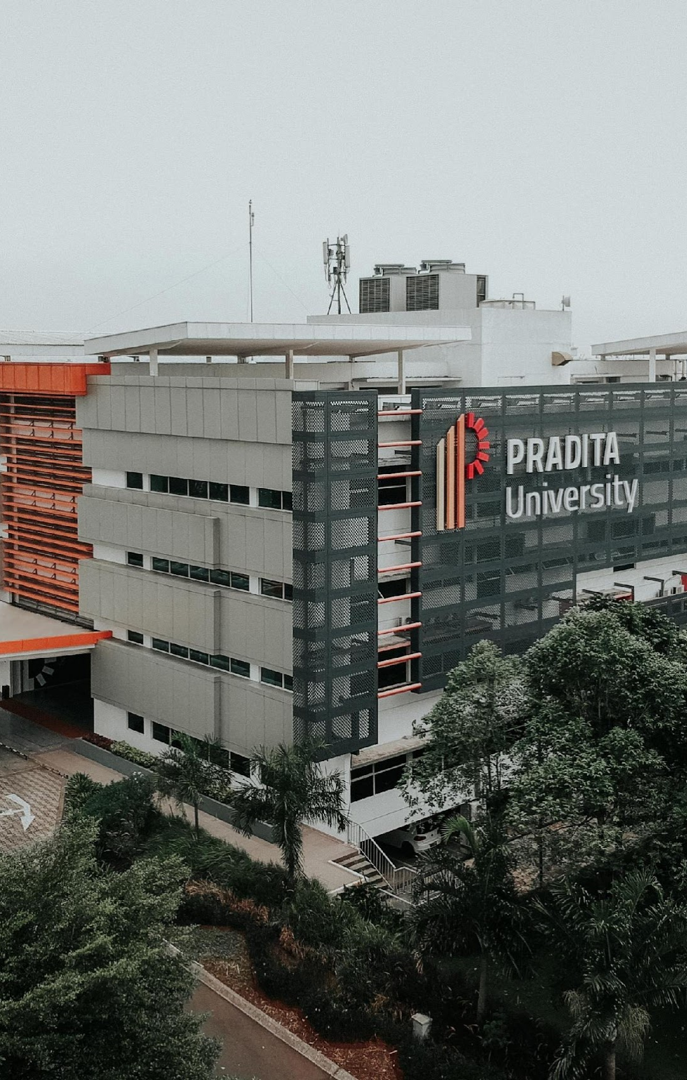
\includegraphics[width=\paperwidth]{../figures/building.png}
		};
		
		% Judul Tengah
		\node[anchor=center] at ([yshift=.1\textheight]current page.center) {
			\begin{minipage}{\textwidth}
				
				{\LARGE \textbf{Course Module -- IT140704}}\\[0.03\textheight] % Book Type
				{\HUGE \textcolor{orange}{\textbf{Big Data for Business}}}\\[.04\textheight] % Title
%				{\Huge \textcolor{orange}{\textbf{Penggunaan Large-language Model}}}\\[.08\textheight] % Subtitle
				{\LARGE \textbf{Alfa Yohannis}}\\[0.05\textheight] % Authors
			\end{minipage}
		};
		
		% Teks bawah dengan latar oranye penuh dan teks putih
		\node[anchor=south west] at (
		current page.south west) {
			\begin{tikzpicture}[remember picture, overlay]
				\node[anchor=south west, fill=orange, text=white, minimum width=\paperwidth, minimum height=.14\textheight, align=center, font=\Huge\bfseries] at (-.15,-.15) {
					Postgraduate Program in Information Technology\\
					Pradita University
				};
			\end{tikzpicture}
		};
	\end{tikzpicture}
\end{titlepage}
	
	% Contents Page
	\tableofcontents
	
	\chapter{Pendahuluan}

\section{Latar Belakang}

Di era transformasi digital saat ini, data telah menjadi aset strategis bagi organisasi di berbagai sektor. Volume data yang terus meningkat, baik dari transaksi internal, interaksi pelanggan, hingga media sosial, menciptakan peluang besar sekaligus tantangan dalam pengambilan keputusan yang efektif dan berbasis bukti. Istilah \textit{big data} mencerminkan kompleksitas data modern yang ditandai oleh karakteristik Volume, Variety, Velocity, Veracity, dan Value (5V).

Bagi kalangan manajerial dan pengambil kebijakan, pemahaman mengenai big data tidak lagi terbatas pada aspek teknis, melainkan lebih pada bagaimana data dapat dimanfaatkan untuk menciptakan nilai bisnis, meningkatkan efisiensi operasional, memahami perilaku konsumen, serta mendukung inovasi berbasis analitik.

\section{Tujuan Pembelajaran}

Mata kuliah ini bertujuan untuk membekali mahasiswa pascasarjana dari latar belakang manajemen dan bisnis dengan pemahaman konseptual dan keterampilan praktis dalam mengelola dan memanfaatkan big data. Tanpa memerlukan latar belakang pemrograman atau teknologi informasi, mahasiswa akan diperkenalkan pada teknologi big data, pendekatan analitik, serta kerangka pengambilan keputusan berbasis data.

Secara khusus, tujuan pembelajaran mencakup:

\begin{itemize}
	\item Memahami konsep, karakteristik, dan peran strategis big data dalam organisasi.
	\item Mampu menjelaskan infrastruktur dan arsitektur teknologi big data secara konseptual.
	\item Menggunakan alat bantu visual (Power BI, Orange, KNIME) untuk eksplorasi data, analisis prediktif, dan visualisasi.
	\item Menganalisis kasus penggunaan big data dalam berbagai sektor industri.
	\item Mengidentifikasi tantangan etika, tata kelola, dan monetisasi data dalam konteks organisasi.
\end{itemize}

\section{Ruang Lingkup Materi}

Materi dalam mata kuliah ini disusun secara bertahap, mencakup empat area pembelajaran utama:

\begin{enumerate}
	\item \textbf{Dasar-dasar dan Strategi Big Data:} pengenalan konsep big data, kerangka kerja strategis seperti \textit{Big Data Value Chain}, \textit{5Vs}, \textit{Big Data Maturity Model} (BDMM), dan arsitektur teknologi data.
	
	\item \textbf{Pengelolaan dan Pemrosesan Data:} mencakup pemahaman basis data (SQL dan NoSQL), proses pembersihan data, dan integrasi sumber data.
	
	\item \textbf{Analisis dan Pengambilan Keputusan:} penggunaan BI dan machine learning untuk segmentasi pelanggan, prediksi perilaku, dan analisis sentimen pelanggan.
	
	\item \textbf{Manfaat, Etika, dan Tata Kelola:} penilaian nilai ekonomi dari data (monetisasi), kerangka kerja pengambilan keputusan berbasis data (CRISP-DM, OSEMN), serta isu etika dan tata kelola data.
\end{enumerate}


\begin{longtable}{|p{0.03\textwidth}|p{0.2\textwidth}|p{0.3\textwidth}|p{0.35\textwidth}|}
	\caption{Course Plan: Big Data for Business (Postgraduate, Management Focus)}\label{tab:course_plan} \\
	\hline
	\textbf{No} & \textbf{Topik} & \textbf{Deskripsi} & \textbf{Frameworks / Tools} \\
	\hline
	\endfirsthead
	
	\multicolumn{4}{c}%
	{{\tablename\ \thetable{} -- lanjutan dari halaman sebelumnya}} \\
	\hline
	\textbf{No} & \textbf{Topik} & \textbf{Deskripsi} & \textbf{Frameworks / Tools} \\
	\hline
	\endhead
	
	\hline \multicolumn{4}{r}{{Bersambung ke halaman berikutnya}} \\
	\endfoot
	
	\hline
	\endlastfoot
	
	1 & Introduction to Big Data in Business & Definitions, business impact, why big data matters & Case study. \\
	\hline
	2 & Big Data Strategy \& Frameworks Overview & Introduce 5Vs, Big Data Value Chain, BDMM, DAMA & -- \\
	\hline
	3 & Big Data Architecture \& Value Chain & End-to-end process: from data sources, ingestion, storage, processing, to BI and analytics presentation & Big Data Value Chain (Capture–Process–Analyse–Visualise–Decide), BDMM, DAMA. Architecture mapping activity. \\
	\hline
	4 & Understanding Databases \& SQL & Structured data and basic querying & Big Data Value Chain (Capture), DAMA (Architecture). SQL tools (DB Fiddle). \\
	\hline
	5 & NoSQL \& Semi-Structured Data & JSON, MongoDB, flexibility in schema design & Big Data Value Chain (Capture), 5Vs (Variety). MongoDB Atlas. \\
	\hline
	6 & Big Data Processing Technologies & Distributed processing frameworks: Hadoop, MapReduce, Spark, Kafka, stream vs batch concepts & Big Data Value Chain (Process–Analyse). Demos of Spark, Hadoop HDFS overview, Kafka stream processing concept. \\
	\hline
	7 & Data Cleaning \& Preparation & Data quality, integration, consistency & Big Data Value Chain (Curate), DAMA (Quality), 5Vs (Veracity). KNIME workflow. \\
	\hline
	8 & Business Intelligence \& Dashboards & KPIs, dashboards, visualisation & Big Data Value Chain (Analyse–Visualise), DAMA. Power BI. \\
	\hline
	9 & Introduction to Machine Learning & ML vs BI, supervised learning & Big Data Value Chain (Analyse), BDMM (Analytics readiness). Orange ML demo. \\
	\hline
	10 & Customer Segmentation (Clustering) & Market segmentation with unsupervised learning & Big Data Value Chain (Analyse), DAMA (Mining), 5Vs (Variety). Orange: k-means. \\
	\hline
	11 & Prediction \& Forecasting & Churn, revenue, or risk prediction & Big Data Value Chain (Analyse–Decide), BDMM. Orange: regression/classification. \\
	\hline
	12 & Text \& Sentiment Analysis & Review/opinion analysis with NLP & Big Data Value Chain (Capture–Analyse), 5Vs (Veracity). Orange: sentiment analysis. \\
	\hline
	13 & Data Monetisation \& Value Realisation & Economic/business value from data & Big Data Value Chain (full chain), BDMM (Value). Value creation strategy. \\
	\hline
	14 & Ethics, Governance \& Maturity Review & Data privacy, governance, ethical use of data & DAMA (Governance), BDMM (Audit). BDMM self-assessment. \\
	\hline
	
\end{longtable}




\section{Metodologi Pembelajaran}

Pembelajaran dilakukan melalui pendekatan interaktif yang menggabungkan ceramah konseptual, studi kasus industri, demonstrasi alat bantu visual, dan latihan praktik berbasis data nyata. Mahasiswa akan bekerja secara individu maupun berkelompok dalam menganalisis permasalahan bisnis dengan pendekatan berbasis data.



\section{Manfaat yang Diharapkan}

Setelah mengikuti mata kuliah ini, mahasiswa diharapkan mampu mengambil peran strategis dalam perencanaan, pengelolaan, dan pemanfaatan data besar untuk mendukung tujuan organisasi. Selain itu, mahasiswa juga memiliki dasar yang kuat untuk memahami dan mengevaluasi proyek transformasi digital berbasis data.


\section{Materi Perkuliahan}

Tabel~\ref{tab:course_plan} menjelaskan struktur 14 pertemuan untuk mata kuliah \textit{Big Data for Business} yang dirancang khusus bagi mahasiswa pascasarjana dari latar belakang manajemen atau non-TIK. Setiap sesi disusun secara bertahap untuk membekali mahasiswa dengan pemahaman praktis mengenai konsep, teknologi, dan penerapan big data dalam konteks organisasi. Materi perkuliahan dibagi ke dalam empat tahapan pembelajaran utama:

\begin{enumerate}
	\item \textbf{Dasar-dasar, Strategi, dan Arsitektur Big Data (Sesi 1--3)} \\
	Mahasiswa diperkenalkan pada konsep dasar big data, kerangka kerja strategis seperti \textit{Big Data Value Chain}, \textit{5Vs}, \textit{BDMM}, serta arsitektur big data end-to-end dari sumber data hingga analitik bisnis.
	
	\item \textbf{Teknologi Pengelolaan dan Pemrosesan Data (Sesi 4--7)} \\
	Fokus pada pemahaman basis data relasional (SQL), data semi-terstruktur (NoSQL), serta teknologi pemrosesan big data seperti Hadoop, MapReduce, Spark, dan Kafka. Termasuk juga pembersihan dan integrasi data menggunakan alat bantu visual seperti KNIME.
	
	\item \textbf{Analitik Bisnis dan Pembelajaran Mesin (Sesi 8--12)} \\
	Mahasiswa mengeksplorasi penerapan \textit{Business Intelligence} menggunakan Power BI, serta pembelajaran mesin (machine learning) menggunakan Orange untuk segmentasi pelanggan, prediksi, dan analisis sentimen.
	
	\item \textbf{Manfaat, Tata Kelola, dan Etika Big Data (Sesi 13--14)} \\
	Tahap akhir mengkaji strategi monetisasi dan realisasi nilai data, serta isu etika, tata kelola data, dan evaluasi kematangan big data melalui pendekatan DAMA dan BDMM.
\end{enumerate}

Kegiatan pembelajaran memanfaatkan pendekatan praktis berbasis alat bantu visual tanpa pemrograman, serta studi kasus dari industri untuk menghubungkan teori dan praktik. Hasil akhir yang diharapkan adalah pemahaman menyeluruh tentang bagaimana data besar mendukung keputusan dan transformasi bisnis dalam berbagai sektor industri.

	\chapter{Pengenalan Big Data untuk Bisnis}


\noindent
Revolusi digital telah menghasilkan volume data yang belum pernah terjadi sebelumnya, yang berasal dari transaksi bisnis, sensor perangkat IoT, interaksi media sosial, hingga sistem informasi internal organisasi. Dalam konteks ini, \textit{big data} muncul bukan hanya sebagai istilah teknologi, melainkan sebagai paradigma baru dalam cara organisasi memahami, mengelola, dan menciptakan nilai dari data. Bab ini akan memperkenalkan konsep dasar big data, menjelaskan karakteristik uniknya, menelaah peran strategisnya dalam dunia usaha, serta mengeksplorasi tantangan dan peluang yang menyertainya di era bisnis digital modern.


\section{Definisi dan Karakteristik Big Data}

Big data merujuk pada kumpulan data dengan volume besar, kecepatan tinggi, dan keragaman format yang melampaui kemampuan sistem pengolahan data konvensional untuk menangkap, mengelola, dan menganalisis secara efisien. Istilah ini pertama kali dipopulerkan dalam konteks teknologi informasi dan bisnis oleh para peneliti dan praktisi untuk menggambarkan ledakan data digital yang terjadi sejak awal abad ke-21.

Salah satu definisi awal dan paling banyak dikutip berasal dari laporan Gartner yang memperkenalkan konsep 3V: \textbf{Volume}, \textbf{Velocity}, dan \textbf{Variety} \cite{laney2001}. Sejak saat itu, berbagai literatur menambahkan karakteristik tambahan seperti \textbf{Veracity} (tingkat kepercayaan terhadap data) dan \textbf{Value} (nilai bisnis yang dapat diperoleh dari data) sehingga menjadi model 5V yang umum digunakan saat ini \cite{gandomi2015}.

Menurut definisi dari National Institute of Standards and Technology (NIST), big data adalah ``data yang melebihi kapasitas atau kemampuan metode saat ini, baik dalam hal akuisisi, penyimpanan, manajemen, dan pemrosesan'' \cite{nist2015}. Standar IEEE P2301 dan ISO/IEC 20547-1 juga menegaskan bahwa big data mencakup aspek infrastruktur, interoperabilitas, serta tata kelola data yang kompleks dalam lingkungan multi-sumber dan multi-format \cite{iso20547}.

Karakteristik utama big data dapat dijelaskan sebagai berikut:

\begin{itemize}
	\item \textbf{Volume:} mencerminkan besarnya ukuran data yang dihasilkan dari berbagai sumber, seperti sensor IoT, transaksi bisnis, media sosial, dan perangkat digital lainnya.
	\item \textbf{Velocity:} menunjukkan kecepatan aliran data masuk ke sistem yang membutuhkan pemrosesan secara real-time atau near-real-time.
	\item \textbf{Variety:} mengacu pada keragaman format data, termasuk data terstruktur, semi-terstruktur (seperti XML dan JSON), dan tidak terstruktur (seperti teks, gambar, video).
	\item \textbf{Veracity:} berkaitan dengan kualitas, keandalan, dan ketidakpastian dari data, termasuk adanya bias, duplikasi, atau noise.
	\item \textbf{Value:} menekankan pentingnya data sebagai aset strategis yang harus dikonversi menjadi wawasan bisnis yang bernilai.
\end{itemize}

Pemahaman terhadap karakteristik ini menjadi dasar bagi pengembangan strategi pengelolaan data yang efektif dalam konteks bisnis modern. Organisasi yang mampu mengidentifikasi dan memanfaatkan karakteristik big data secara tepat dapat memperoleh keunggulan kompetitif yang signifikan \cite{wamba2017}.



\section{Peran Strategis Big Data dalam Organisasi}

Big data memiliki peran strategis dalam mendukung transformasi digital, meningkatkan efisiensi operasional, memahami pelanggan secara mendalam, dan menciptakan nilai bisnis baru. Lebih dari sekadar kumpulan data berukuran besar, big data memungkinkan organisasi untuk mengubah data menjadi wawasan (\textit{insight}) yang dapat ditindaklanjuti secara real-time maupun jangka panjang.

Menurut McAfee dan Brynjolfsson (2012), organisasi yang mengadopsi pendekatan berbasis data dalam pengambilan keputusan memiliki kemungkinan 5\% lebih produktif dan 6\% lebih menguntungkan dibandingkan dengan kompetitor yang mengandalkan intuisi semata \cite{mcafee2012}. Big data menjadi tulang punggung bagi strategi perusahaan modern dalam mendukung inovasi berbasis informasi, peningkatan layanan pelanggan, serta pengambilan keputusan yang lebih cepat dan presisi.

Secara umum, peran strategis big data dalam organisasi mencakup lima area utama:

\begin{enumerate}
	\item \textbf{Pengambilan Keputusan yang Lebih Baik:} Data analitik memungkinkan manajemen untuk mengambil keputusan berdasarkan fakta dan pola historis, bukan hanya intuisi atau asumsi \cite{chen2012}.
	
	\item \textbf{Optimalisasi Operasional:} Big data dapat digunakan untuk mendeteksi inefisiensi, mengurangi biaya, serta mengotomatiskan proses bisnis melalui sistem prediktif dan preskriptif \cite{waller2013}.
	
	\item \textbf{Pengenalan Pasar dan Pelanggan:} Analisis big data memungkinkan segmentasi pelanggan yang lebih tajam, personalisasi layanan, dan peramalan tren perilaku secara real-time \cite{jeble2018}.
	
	\item \textbf{Inovasi Produk dan Model Bisnis:} Organisasi dapat mengembangkan produk berbasis data dan menciptakan model bisnis baru seperti layanan berbasis langganan, rekomendasi cerdas, dan penawaran berbasis lokasi \cite{mariani2021}.
	
	\item \textbf{Keunggulan Kompetitif:} Big data membantu organisasi menanggapi perubahan pasar dengan lebih cepat dan akurat, sehingga menciptakan diferensiasi yang berkelanjutan \cite{georgescu2020}.
\end{enumerate}

Lembaga internasional seperti OECD juga menekankan bahwa adopsi big data harus dibarengi dengan kesiapan tata kelola, infrastruktur, dan budaya organisasi yang mendukung pengambilan keputusan berbasis data \cite{oecd2015}. Oleh karena itu, peran strategis big data tidak hanya bersifat teknis, tetapi juga menyangkut aspek manajerial, kebijakan, dan kapabilitas organisasi secara menyeluruh.


\section{Evolusi Teknologi dan Konteks Bisnis Digital}

Perkembangan teknologi informasi dan komunikasi dalam dua dekade terakhir telah mengubah lanskap bisnis secara fundamental. Organisasi saat ini beroperasi dalam lingkungan yang semakin terdigitalisasi, terdorong oleh konektivitas global, otomatisasi proses, dan munculnya platform digital. Dalam konteks ini, big data menjadi elemen kunci yang mendukung pengambilan keputusan yang cepat dan berbasis fakta, serta mendorong inovasi di berbagai lini bisnis.

Evolusi teknologi big data tidak terjadi secara terisolasi, tetapi merupakan bagian dari ekosistem transformasi digital yang lebih luas. Pergeseran dari sistem informasi tradisional menuju platform data modern mencakup beberapa tonggak penting:

\begin{itemize}
	\item \textbf{Era Warehouse (1980–2000):} Fokus pada data historis terstruktur melalui sistem data warehouse dan OLAP untuk pelaporan manajerial.
	
	\item \textbf{Era Web dan Cloud (2000–2010):} Munculnya aplikasi web, komputasi awan, dan sensor digital meningkatkan volume dan kecepatan data yang perlu diproses.
	
	\item \textbf{Era Big Data (2010–sekarang):} Diperkenalkannya teknologi Hadoop, MapReduce, dan kemudian Apache Spark memungkinkan pemrosesan data skala besar secara terdistribusi dan paralel \cite{assuncao2015, jagadish2014}.
	
	\item \textbf{Era AI dan Real-Time Analytics (2018–kini):} Integrasi antara big data, kecerdasan buatan, dan analitik waktu nyata telah menghasilkan sistem cerdas untuk pengambilan keputusan otomatis, seperti rekomendasi produk, deteksi fraud, dan prediksi permintaan \cite{davenport2018, fernandez2020}.
\end{itemize}

Dalam lingkungan bisnis digital, data tidak hanya diproses secara pasif, tetapi menjadi sumber keunggulan kompetitif yang aktif. Strategi digital modern mengintegrasikan big data ke dalam proses bisnis inti, seperti manajemen rantai pasok, pemasaran digital, personalisasi layanan pelanggan, hingga perencanaan strategis berbasis data.

Menurut laporan World Economic Forum (WEF), data telah menjadi faktor produksi baru di era ekonomi digital, sejajar dengan tenaga kerja dan modal \cite{wef2016}. Hal ini menuntut organisasi untuk tidak hanya memiliki infrastruktur teknologi yang memadai, tetapi juga kemampuan analitik, tata kelola data, serta budaya organisasi yang mendukung eksplorasi dan eksploitasi data secara optimal.



\section{Tantangan dan Peluang dalam Pemanfaatan Big Data}

Meskipun big data menawarkan potensi besar untuk menciptakan nilai bisnis, penerapannya dalam organisasi tidak bebas hambatan. Berbagai tantangan muncul, baik dari aspek teknis, organisasional, maupun etis. Namun demikian, tantangan ini sekaligus membuka ruang bagi inovasi dan pengembangan strategi manajemen data yang lebih matang dan berkelanjutan.

\subsection*{Tantangan dalam Pemanfaatan Big Data}

\begin{enumerate}
	\item \textbf{Kualitas dan Integrasi Data:} Data yang berasal dari berbagai sumber internal dan eksternal sering kali tidak konsisten, memiliki format yang berbeda, atau mengandung informasi yang tidak lengkap. Menurut penelitian oleh Sadiq et al. (2017), isu kualitas data merupakan penghambat utama dalam keberhasilan inisiatif analitik data \cite{sadiq2017}.
	
	\item \textbf{Kekurangan Talenta dan Kapabilitas Analitik:} Banyak organisasi mengalami kesenjangan keterampilan antara kebutuhan analitik lanjutan dan ketersediaan sumber daya manusia yang mampu memahami dan mengolah data dalam skala besar \cite{deloitte2021}.
	
	\item \textbf{Ketidakjelasan Strategi Data:} Beberapa organisasi menerapkan teknologi big data tanpa peta jalan strategis yang jelas, sehingga inisiatif data tidak terhubung langsung dengan tujuan bisnis \cite{schroeck2012}.
	
	\item \textbf{Risiko Keamanan dan Privasi:} Volume besar data personal dan sensitif meningkatkan eksposur terhadap risiko kebocoran dan penyalahgunaan data. Hal ini menjadi perhatian penting dalam konteks regulasi seperti GDPR dan UU Perlindungan Data Pribadi \cite{zwitter2014}.
	
	\item \textbf{Isu Tata Kelola dan Etika Data:} Tantangan terkait siapa yang bertanggung jawab atas akurasi, penggunaan, dan penyimpanan data kerap tidak terdefinisi dengan baik dalam organisasi, terutama pada institusi yang belum memiliki struktur tata kelola data formal \cite{otieno2021}.
\end{enumerate}

\subsection*{Peluang Strategis dari Big Data}

Meskipun menghadapi berbagai tantangan, big data tetap menjadi enabler utama bagi transformasi bisnis. Beberapa peluang yang dapat dimanfaatkan organisasi antara lain:

\begin{itemize}
	\item \textbf{Peningkatan Efisiensi Operasional:} Dengan kemampuan prediksi dan otomasi berbasis data, organisasi dapat mengoptimalkan rantai pasok, manajemen stok, dan alokasi sumber daya \cite{george2014}.
	
	\item \textbf{Pemahaman Pelanggan yang Lebih Dalam:} Analisis perilaku pelanggan, preferensi, dan umpan balik memungkinkan penyusunan strategi pemasaran yang lebih personal dan efektif.
	
	\item \textbf{Inovasi Produk dan Layanan:} Big data menjadi sumber insight untuk pengembangan produk baru berbasis kebutuhan dan tren pasar yang sedang berkembang.
	
	\item \textbf{Pengambilan Keputusan Real-Time:} Integrasi antara big data, machine learning, dan sistem dashboard memungkinkan pengambilan keputusan instan dalam konteks operasional maupun strategis \cite{russom2011}.
	
	\item \textbf{Monetisasi Data:} Data internal organisasi dapat menjadi aset yang bernilai tinggi melalui strategi seperti \textit{data-as-a-service}, model berbasis langganan, atau kerja sama data antar perusahaan \cite{labreuche2020}.
\end{itemize}

Oleh karena itu, penting bagi organisasi untuk mengembangkan kerangka kerja yang menyelaraskan aspek teknologi, manusia, proses, dan tata kelola data agar dapat meminimalkan risiko sekaligus mengoptimalkan peluang strategis dari pemanfaatan big data.


\section{Contoh Penerapan Big Data di Dunia Usaha}

Pemanfaatan big data telah merambah hampir seluruh sektor industri, mulai dari ritel, keuangan, logistik, hingga kesehatan dan pendidikan. Dalam dunia usaha, big data digunakan untuk meningkatkan efisiensi operasional, memperkuat hubungan dengan pelanggan, mengoptimalkan strategi pemasaran, serta menciptakan inovasi berbasis data.

Berikut adalah beberapa contoh penerapan big data dalam dunia usaha:

\subsection*{1. Ritel dan E-commerce}

Perusahaan seperti Amazon dan Tokopedia menggunakan big data untuk menganalisis perilaku belanja konsumen secara real-time, membangun sistem rekomendasi produk, dan mengoptimalkan manajemen rantai pasok. Sistem rekomendasi berbasis machine learning memanfaatkan data histori pembelian, pencarian, dan interaksi pelanggan untuk meningkatkan tingkat konversi penjualan \cite{mcafee2012, sun2019}.

\subsection*{2. Keuangan dan Perbankan}

Di sektor perbankan, big data digunakan untuk deteksi fraud, analisis risiko kredit, dan personalisasi penawaran layanan. Algoritma big data dapat mendeteksi anomali transaksi secara real-time dan memberikan notifikasi pencegahan terhadap aktivitas mencurigakan. Fintech juga memanfaatkan data sosial dan data alternatif lainnya untuk menilai kelayakan kredit nasabah yang tidak memiliki histori keuangan formal \cite{lee2019, goyal2022}.

\subsection*{3. Manufaktur dan Industri 4.0}

Industri manufaktur mengintegrasikan big data dengan sensor Internet of Things (IoT) untuk memantau kondisi mesin, melakukan pemeliharaan prediktif, dan meningkatkan efisiensi proses produksi. Konsep smart factory dalam Industry 4.0 sangat bergantung pada data sensor, machine learning, dan analitik visual untuk mengoptimalkan kinerja operasional \cite{lee2015, ghobakhloo2018}.

\subsection*{4. Transportasi dan Logistik}

Perusahaan seperti Gojek dan FedEx memanfaatkan data lokasi, cuaca, dan pola permintaan pelanggan untuk mengoptimalkan rute pengiriman dan waktu tempuh secara real-time. Big data juga digunakan untuk melakukan analisis prediktif terhadap lonjakan permintaan layanan transportasi \cite{zheng2016}.

\subsection*{5. Kesehatan dan Layanan Publik}

Dalam layanan kesehatan, big data digunakan untuk deteksi dini penyakit, analisis tren kesehatan populasi, dan pengembangan pengobatan personal (precision medicine). Rumah sakit dan penyedia layanan kesehatan mengandalkan analitik data rekam medis elektronik untuk pengambilan keputusan klinis yang lebih baik \cite{ristevski2018}.

\subsection*{6. Pendidikan dan Learning Analytics}

Institusi pendidikan menggunakan big data untuk mengukur kinerja belajar mahasiswa, menganalisis interaksi pembelajaran daring, dan mengembangkan sistem pembelajaran adaptif. Analitik pembelajaran (learning analytics) membantu dosen dan administrator dalam merancang intervensi akademik yang lebih tepat sasaran \cite{papamitsiou2014}.

Penerapan big data dalam berbagai sektor ini menunjukkan bahwa data telah menjadi sumber daya strategis baru dalam mendukung inovasi dan keunggulan kompetitif. Keberhasilan implementasi bergantung pada kesiapan teknologi, tata kelola, budaya organisasi, dan kompetensi SDM yang mendukung transformasi digital.

\section{Penutup}

Bab ini telah memberikan gambaran umum mengenai konsep dasar big data dan peran strategisnya dalam dunia bisnis. Dimulai dari definisi dan karakteristik teknisnya yang khas, big data dipahami sebagai kumpulan data dalam skala besar yang ditandai oleh lima dimensi utama: volume, velocity, variety, veracity, dan value. Karakteristik ini menuntut pendekatan dan teknologi yang berbeda dari sistem informasi konvensional, baik dalam hal pengumpulan, penyimpanan, maupun analisis data.

Lebih dari sekadar fenomena teknologi, big data memiliki dampak transformasional terhadap model bisnis, proses pengambilan keputusan, dan strategi organisasi. Organisasi yang mampu mengelola dan memanfaatkan data secara efektif dapat memperoleh keunggulan kompetitif yang signifikan, mulai dari peningkatan efisiensi operasional hingga inovasi berbasis informasi.

Perkembangan teknologi yang mendukung big data—seperti komputasi awan, Internet of Things (IoT), dan kecerdasan buatan—menempatkan big data sebagai fondasi utama dalam ekosistem bisnis digital modern. Namun demikian, pemanfaatan big data juga membawa berbagai tantangan, baik dalam hal tata kelola, keamanan, etika, maupun kesiapan sumber daya manusia.

Contoh penerapan di berbagai sektor menunjukkan bahwa nilai dari big data tidak hanya bergantung pada teknologi yang digunakan, tetapi juga pada keselarasan antara strategi bisnis, proses organisasi, dan budaya berbasis data. Oleh karena itu, pemahaman terhadap konteks bisnis dan pengambilan keputusan berbasis data menjadi kompetensi kunci dalam menghadapi era ekonomi digital.

Bab-bab berikutnya akan membahas secara lebih rinci bagaimana organisasi dapat mengelola siklus hidup data, memilih infrastruktur yang tepat, serta menerapkan analitik data untuk menjawab tantangan nyata di berbagai bidang industri.

	\chapter{Strategi dan Kerangka Kerja Big Data}

\noindent
Implementasi big data yang sukses dalam organisasi tidak cukup hanya mengandalkan teknologi canggih atau volume data yang besar. Diperlukan pendekatan strategis yang menyeluruh agar data dapat diolah dan dimanfaatkan secara efektif untuk mendukung tujuan bisnis. Strategi big data berfungsi sebagai fondasi dalam merencanakan, mengelola, dan mengevaluasi inisiatif data di seluruh unit organisasi. Dalam bab ini, akan dibahas berbagai kerangka kerja penting yang digunakan untuk memahami dan membangun strategi big data secara sistematis, termasuk model 5Vs, Big Data Value Chain, Big Data Maturity Model (BDMM), serta kerangka tata kelola DAMA-DMBOK. Kerangka-kerangka ini tidak hanya memberikan panduan konseptual, tetapi juga membantu organisasi dalam mengukur kesiapan, menetapkan prioritas, dan mengelola siklus hidup data secara strategis.


\section{Pentingnya Strategi Big Data dalam Organisasi}

Strategi big data merupakan pendekatan terencana dan terstruktur yang dirancang untuk memaksimalkan pemanfaatan data dalam mencapai tujuan bisnis. Di tengah meningkatnya volume, variasi, dan kecepatan data yang masuk ke organisasi, keberadaan strategi yang jelas menjadi faktor penentu keberhasilan implementasi big data secara berkelanjutan dan berdampak nyata.

Tanpa strategi, organisasi sering kali terjebak dalam inisiatif teknologi yang terfragmentasi, tidak selaras dengan prioritas bisnis, serta menghasilkan beban biaya tinggi tanpa hasil yang signifikan. Gartner (2018) melaporkan bahwa lebih dari 85\% proyek big data gagal memberikan nilai bisnis karena kurangnya penyelarasan antara teknologi, proses bisnis, dan kompetensi organisasi \cite{gartner2018}.

Strategi big data yang efektif mencakup beberapa elemen utama:
\begin{enumerate}
	\item \textbf{Visi dan Tujuan Bisnis:} Strategi harus dimulai dari pemahaman tujuan bisnis, seperti meningkatkan loyalitas pelanggan, efisiensi rantai pasok, atau inovasi produk berbasis data.
	
	\item \textbf{Arsitektur dan Teknologi:} Pemilihan platform dan infrastruktur yang sesuai dengan skala, kecepatan, dan kebutuhan integrasi data organisasi sangat krusial dalam mendukung strategi data yang berkelanjutan \cite{ekambaram2021}.
	
	\item \textbf{Tata Kelola dan Kepatuhan:} Strategi harus mengatur bagaimana data dikumpulkan, disimpan, diakses, dan digunakan dengan mematuhi kebijakan privasi dan etika \cite{otieno2021}.
	
	\item \textbf{Kapabilitas Organisasi:} Pengembangan kompetensi internal, pelatihan, dan pembentukan budaya berbasis data menjadi fondasi pelaksanaan strategi secara menyeluruh \cite{lewis2021}.
	
	\item \textbf{Metrik dan Evaluasi Dampak:} Strategi perlu menetapkan indikator kinerja untuk mengukur efektivitas inisiatif data, baik dari sisi operasional, finansial, maupun inovasi.
\end{enumerate}

Dalam konteks yang lebih luas, strategi big data juga berfungsi sebagai jembatan antara visi digital organisasi dan pelaksanaannya melalui teknologi. Menurut laporan McKinsey, perusahaan yang mengintegrasikan strategi data dengan pengambilan keputusan tingkat manajemen cenderung lebih adaptif dan unggul dalam bersaing di era digital \cite{mckinsey2016}.

Oleh karena itu, strategi big data bukan sekadar rencana teknis, tetapi merupakan bagian integral dari transformasi organisasi menuju pengambilan keputusan berbasis bukti, efisiensi proses, dan inovasi yang berkelanjutan.

\section{Kerangka Konseptual 5Vs Big Data}

Kerangka 5Vs merupakan salah satu model konseptual yang paling umum digunakan untuk menjelaskan kompleksitas dan tantangan pengelolaan big data. Diperkenalkan pertama kali oleh Doug Laney (2001) dengan tiga elemen awal—Volume, Velocity, dan Variety—kerangka ini kemudian diperluas dengan Veracity dan Value oleh peneliti dan praktisi industri \cite{laney2001, gandomi2015}. Setiap dimensi mencerminkan karakteristik unik data modern yang harus dipertimbangkan dalam perencanaan strategi data organisasi.

\subsection{Volume}

Volume merujuk pada skala besar data yang dikumpulkan dan disimpan oleh organisasi. Peningkatan volume data berasal dari beragam sumber seperti sistem transaksi, log aktivitas pengguna, sensor IoT, media sosial, hingga rekam medis elektronik. Menurut IDC (2021), total data digital global diperkirakan mencapai lebih dari 180 zettabytes pada tahun 2025 \cite{idc2021}. Volume besar ini menuntut penggunaan sistem penyimpanan terdistribusi seperti Hadoop HDFS atau penyimpanan awan dengan skala elastis.

Sebagai contoh, perusahaan e-commerce seperti Amazon menangani miliaran permintaan produk, klik pengguna, dan transaksi per hari yang harus disimpan dan diproses secara efisien untuk kebutuhan analitik dan layanan personalisasi. Di sektor kesehatan, rumah sakit dan penyedia layanan kesehatan menghasilkan data medis dalam jumlah besar, seperti hasil laboratorium, rekam radiologi, dan catatan elektronik pasien, yang semuanya harus disimpan dengan aman dan sesuai standar regulasi.

\subsection{Velocity}

Velocity mengacu pada kecepatan data dihasilkan, ditransmisikan, dan diproses. Dalam konteks bisnis modern, kemampuan memproses data secara real-time atau near-real-time menjadi sangat penting, misalnya dalam sistem rekomendasi online, deteksi fraud perbankan, atau monitoring kondisi mesin. Teknologi seperti Apache Kafka dan Spark Streaming memungkinkan organisasi merespons data streaming dengan latensi rendah \cite{demchenko2013}.

Contoh nyata dari penerapan velocity adalah sistem navigasi transportasi daring seperti Gojek atau Grab yang memproses data lokasi jutaan pengguna dan pengemudi secara real-time untuk mengatur alokasi armada dan estimasi waktu kedatangan. Contoh lain adalah sistem perdagangan saham algoritmik yang harus memproses dan merespons data pasar dalam milidetik untuk mengeksekusi keputusan pembelian atau penjualan secara otomatis.


\subsection{Variety}

Variety menjelaskan keragaman jenis dan format data. Data modern tidak hanya berupa data terstruktur dalam tabel relasional, tetapi juga mencakup data semi-terstruktur (seperti XML dan JSON), serta data tidak terstruktur seperti teks, gambar, audio, dan video. Perusahaan yang mampu menggabungkan data dari berbagai format dapat memperoleh wawasan yang lebih menyeluruh dan holistik \cite{gandomi2015}.

Sebagai contoh, platform media sosial seperti Facebook dan TikTok memproses berbagai jenis data termasuk teks status, metadata pengguna, komentar suara, foto, serta video pendek. Penggabungan data ini memungkinkan algoritma rekomendasi bekerja lebih akurat dalam memahami preferensi pengguna. Di sektor layanan pelanggan, perusahaan seperti Telkom atau PLN menggabungkan data terstruktur dari sistem billing dengan data tidak terstruktur dari log percakapan call center untuk meningkatkan kualitas layanan dan merespon keluhan secara proaktif.

\subsection{Veracity}

Veracity berhubungan dengan akurasi, konsistensi, dan keandalan data. Data yang mengandung noise, inkonsistensi, atau bias dapat menghasilkan kesimpulan yang salah dan berdampak negatif pada keputusan bisnis. Oleh karena itu, proses validasi, pembersihan data, dan pengelolaan metadata menjadi komponen penting dalam manajemen data modern \cite{sadiq2017}.

Sebagai contoh, dalam industri kesehatan, kesalahan input dalam data rekam medis pasien seperti usia, alergi, atau riwayat obat dapat mengakibatkan diagnosis yang tidak akurat dan membahayakan nyawa pasien. Di sektor keuangan, data nasabah yang tidak konsisten antar sistem—misalnya perbedaan ejaan nama atau alamat—dapat menyebabkan duplikasi profil atau kesalahan scoring risiko kredit. Oleh karena itu, verifikasi, normalisasi, dan deduplikasi data menjadi prosedur wajib dalam proyek integrasi data lintas sistem.

\subsection{Value}

Value adalah tujuan akhir dari seluruh inisiatif big data—yakni menciptakan nilai nyata bagi organisasi. Data yang besar dan cepat tidak memiliki arti tanpa penerapan analitik dan interpretasi yang tepat. Nilai dapat dihasilkan dalam bentuk peningkatan efisiensi, pengurangan biaya, peningkatan kepuasan pelanggan, atau penciptaan model bisnis baru \cite{waller2013}. Oleh karena itu, strategi big data harus berorientasi pada nilai, bukan hanya volume teknis.

Sebagai contoh, Netflix menggunakan big data untuk menganalisis perilaku tontonan penggunanya secara real-time, yang kemudian diterjemahkan menjadi strategi rekomendasi konten yang sangat personal. Pendekatan ini tidak hanya meningkatkan waktu tonton dan retensi pelanggan, tetapi juga digunakan dalam pengambilan keputusan produksi serial orisinal, seperti dalam kasus sukses “House of Cards.”

Contoh lain datang dari industri logistik: perusahaan seperti DHL atau Maersk memanfaatkan analitik big data untuk mengoptimalkan rute pengiriman, meminimalkan waktu tempuh, serta mengurangi konsumsi bahan bakar dan emisi karbon. Hasilnya adalah peningkatan efisiensi operasional sekaligus kontribusi terhadap tujuan keberlanjutan (sustainability) perusahaan.

\begin{longtable}{|p{0.1\textwidth}|p{0.34\textwidth}|p{0.47\textwidth}|}
	\caption{Ringkasan 5Vs dalam Kerangka Konseptual Big Data}
	\label{tab:5vs} \\
	\hline
	\textbf{Dimensi} & \textbf{Deskripsi} & \textbf{Contoh Aplikasi Nyata} \\
	\hline
	\endfirsthead
	
	\multicolumn{3}{c}{{\tablename\ \thetable{} -- lanjutan dari halaman sebelumnya}} \\
	\hline
	\textbf{Dimensi} & \textbf{Deskripsi} & \textbf{Contoh Aplikasi Nyata} \\
	\hline
	\endhead
	
	\hline \multicolumn{3}{r}{{Bersambung ke halaman berikutnya}} \\
	\endfoot
	
	\hline
	\endlastfoot
	
	\textbf{Volume} & Skala besar data yang dikumpulkan dari berbagai sumber, seperti transaksi, sensor IoT, media sosial, dan rekam medis. & Amazon menangani miliaran transaksi dan klik; rumah sakit menyimpan data laboratorium, radiologi, dan rekam medis dalam jumlah besar. \\
	\hline
	\textbf{Velocity} & Kecepatan data dihasilkan dan diproses secara real-time atau near-real-time. & Gojek memproses data lokasi jutaan pengguna secara langsung; algoritma saham mengeksekusi transaksi dalam hitungan milidetik. \\
	\hline
	\textbf{Variety} & Keragaman format data: terstruktur, semi-terstruktur (XML/JSON), dan tidak terstruktur (teks, audio, video). & TikTok menggabungkan metadata, video, dan komentar suara; Telkom memadukan data billing dengan log percakapan pelanggan. \\
	\hline
	\textbf{Veracity} & Tingkat keakuratan, konsistensi, dan keandalan data, serta pengelolaan noise dan bias. & Kesalahan input data medis dapat membahayakan diagnosis; duplikasi data nasabah menyebabkan kesalahan scoring risiko kredit. \\
	\hline
	\textbf{Value} & Nilai bisnis yang dihasilkan melalui analitik, seperti efisiensi, penghematan biaya, atau inovasi. & Netflix meningkatkan retensi dengan rekomendasi konten personal; DHL mengoptimalkan rute dan efisiensi logistik menggunakan data. \\
	\hline
	
\end{longtable}



Kerangka 5Vs (Tabel~\ref{tab:5vs}) memberikan dasar konseptual yang berguna untuk mengevaluasi kesiapan organisasi dalam memanfaatkan big data serta membantu merumuskan pendekatan yang tepat dalam perencanaan, integrasi, dan penggunaan data dalam konteks bisnis.

\section{Big Data Value Chain}

Salah satu pendekatan kerangka kerja yang banyak digunakan dalam strategi big data adalah model \textit{Big Data Value Chain}. Dalam kajian ini, rantai nilai data dioperasionalkan ke dalam delapan langkah praktis: \textbf{Capture}, \textbf{Curate}, \textbf{Process}, \textbf{Analyse}, \textbf{Visualise}, \textbf{Decide}, \textbf{Act}, dan \textbf{Measure}. Struktur ini merupakan adaptasi dari berbagai sumber termasuk Open Data Watch \cite{opendatawatch2020}, Curry \cite{curry2016}, dan McKinsey \cite{mckinsey2021}, serta mempertimbangkan prinsip-prinsip dari TDWI \cite{tdwi2013}, CRISP-DM \cite{crispdm1999}, dan Forrester \cite{forrester2016}. Penambahan tahap \textit{Act} dan \textit{Measure} mencerminkan pentingnya pelaksanaan serta evaluasi berkelanjutan dari keputusan berbasis data. Setiap tahapan berkontribusi dalam siklus nilai data secara utuh dari pengumpulan hingga pengukuran dampak.

\subsection{Tahapan: Capture, Curate, Process, Analyse, Visualise, Decide, Act, Measure}


\begin{enumerate}
	\item \textbf{Define}. Tahap penetapan tujuan bisnis, kebutuhan data, dan pertanyaan analitik yang ingin dijawab. Aktivitas ini memastikan bahwa proses data yang dilakukan selaras dengan strategi organisasi dan menghasilkan insight yang relevan. \textit{Contoh:} menentukan apa yang akan dianalisis, data yang perlu di-tangkap, teknologi yang diperlukan, metode analisis yang tepat, dsb. Dokumen: business case, data requirement specification, analisis kebutuhan.
	
	\item \textbf{Capture}. Tahap pengumpulan data dari berbagai sumber internal maupun eksternal, baik terstruktur maupun tidak terstruktur. Data dapat berasal dari transaksi pelanggan, sensor IoT, media sosial, log sistem, atau sumber pihak ketiga. \textit{Contoh:} sensor IoT, log sistem, transaksi pelanggan. Teknologi: API, web scraping, Apache NiFi.
	
	\item \textbf{Curate}. Tahapan ini mencakup proses pembersihan, validasi, standarisasi, serta integrasi data agar siap digunakan dalam analisis. Kualitas dan konsistensi data ditingkatkan agar dapat digunakan lintas sistem dan fungsi. \textit{Contoh:} penghapusan duplikasi, validasi format, harmonisasi nilai kategori. Tools: KNIME, Talend, Alteryx.
	
	\item \textbf{Process}. Transformasi data ke dalam format yang sesuai untuk kebutuhan analisis, serta penyimpanan dalam infrastruktur yang mendukung skalabilitas dan akses cepat. Termasuk proses ETL (Extract, Transform, Load), pemrosesan batch, atau real-time. \textit{Contoh:} pemrosesan data harian dengan Hadoop, pemantauan log real-time menggunakan Spark Streaming. Tools: Hadoop, Spark, Airflow.
	
	\item \textbf{Analyse}. Data yang telah diproses kemudian dieksplorasi dan dianalisis untuk menemukan pola, anomali, atau insight menggunakan teknik statistik maupun machine learning. Analisis ini dapat bersifat deskriptif, diagnostik, prediktif, atau preskriptif. \textit{Contoh:} prediksi churn pelanggan, segmentasi pasar, analisis hubungan antar variabel. Tools: Orange, scikit-learn, RapidMiner, R, Python.
	
	\item \textbf{Visualise}. Penyajian hasil analisis dalam bentuk grafis dan visual interaktif untuk mendukung pemahaman, komunikasi, dan pengambilan keputusan. Visualisasi yang baik mempermudah interpretasi insight oleh pemangku kepentingan non-teknis. \textit{Contoh:} dashboard penjualan harian di Power BI, visualisasi klaster pelanggan di Tableau.
	
	\item \textbf{Decide}. Tahapan pengambilan keputusan berbasis data yang telah dianalisis. Keputusan dapat bersifat operasional (seperti penyesuaian stok otomatis), taktis (penargetan kampanye), hingga strategis (pengembangan layanan baru). \textit{Contoh:} strategi penetapan harga dinamis, pemilihan prioritas fitur produk.
	
	\item \textbf{Act}. Implementasi dari keputusan yang telah diambil ke dalam proses bisnis nyata. Tahap ini memastikan bahwa insight yang diperoleh tidak hanya berhenti di level analisis, namun diintegrasikan dalam operasional organisasi. \textit{Contoh:} peluncuran kampanye pemasaran otomatis, aktivasi sistem rekomendasi produk, penyesuaian jadwal distribusi logistik.
	
	\item \textbf{Measure}. Evaluasi terhadap dampak dari tindakan yang diambil guna mengukur efektivitas, efisiensi, dan nilai tambah dari penggunaan data. Hasil evaluasi menjadi dasar untuk iterasi perbaikan strategi data di masa depan. \textit{Contoh:} pengukuran ROI kampanye, analisis perbandingan A/B testing, pelacakan akurasi model prediksi, dashboard KPI performa unit bisnis.
\end{enumerate}


Kerangka ini tidak hanya menjelaskan bagaimana data diproses secara teknis, tetapi juga menekankan pentingnya nilai bisnis dari setiap tahapan. Tabel~\ref{tab:big_data_value_chain} merangkum tiap tahapan.

\begin{longtable}{|p{0.11\textwidth}|p{0.82\textwidth}|}
	\caption{Tahapan dalam Big Data Value Chain}
	\label{tab:big_data_value_chain} \\
	\hline
	\textbf{Tahapan} & \textbf{Deskripsi dan Contoh} \\
	\hline
	\endfirsthead
	
	\multicolumn{2}{c}{{\tablename\ \thetable{} -- lanjutan dari halaman sebelumnya}} \\
	\hline
	\textbf{Tahapan} & \textbf{Deskripsi dan Contoh} \\
	\hline
	\endhead
	
	\hline \multicolumn{2}{r}{{Bersambung ke halaman berikutnya}} \\
	\endfoot
	
	\hline
	\endlastfoot
	
	\textbf{Capture} &
	Pengumpulan data dari berbagai sumber internal dan eksternal, baik terstruktur maupun tidak terstruktur. \textit{Contoh:}  transaksi pelanggan, log sistem, sensor IoT, media sosial. Teknologi: API, web scraping, Apache NiFi. \\
	\hline
	\textbf{Curate} &
	Pembersihan, filter, dan integrasi data untuk memastikan kualitas dan konsistensi. Contoh aktivitas: penghapusan duplikasi, standarisasi format. Tools: KNIME, Talend, Alteryx. \\
	\hline
	\textbf{Process} &
	Transformasi dan penyimpanan data agar siap dianalisis. Meliputi pemrosesan batch (Hadoop) atau real-time (Spark). Pilihan bergantung pada volume dan kebutuhan bisnis. \\
	\hline
	\textbf{Analyse} &
	Analisis data untuk menemukan pola dan insight. Pendekatan statistik dan machine learning digunakan. Tools: Orange, scikit-learn, RapidMiner. \\
	\hline
	\textbf{Visualise} &
	Penyajian hasil analisis dalam bentuk visualisasi informatif dan interaktif. \textit{Contoh:}  dashboard Power BI, Tableau untuk mendukung interpretasi bisnis. \\
	\hline
	\textbf{Decide} &
	Pengambilan keputusan berbasis data. Dapat berupa keputusan operasional (pengaturan stok), taktis (kampanye), atau strategis (pengembangan produk). \\
	\hline
	
\end{longtable}


\subsection{Aplikasi Value Chain dalam Konteks Bisnis}

Model Big Data Value Chain sangat relevan dalam berbagai sektor industri. Beberapa contoh aplikatif meliputi:

\begin{itemize}
	\item \textbf{Ritel dan E-commerce:} Perusahaan seperti Tokopedia atau Shopee menangkap data klik dan transaksi (\textit{capture}), membersihkannya dari bot dan error (\textit{curate}), memproses dalam data warehouse (\textit{process}), menganalisis perilaku pengguna (\textit{analyse}), menampilkan rekomendasi produk (\textit{visualise}), dan secara otomatis mempersonalisasi halaman utama pelanggan (\textit{decide}).
	
	\item \textbf{Manufaktur:} Dalam industri manufaktur, sensor pada mesin produksi menangkap data suhu dan getaran (\textit{capture}), data dikurasi agar hanya anomali penting yang disimpan (\textit{curate}), dilakukan proses normalisasi data IoT (\textit{process}), lalu digunakan untuk model prediksi kerusakan mesin (\textit{analyse}). Hasil ditampilkan melalui dashboard kondisi mesin (\textit{visualise}) untuk mendukung keputusan pemeliharaan prediktif (\textit{decide}).
	
	\item \textbf{Keuangan:} Di sektor perbankan, aliran transaksi digital (\textit{capture}) dikurasi untuk menyingkirkan noise dan error (\textit{curate}), diproses secara real-time dengan streaming analytics (\textit{process}), dianalisis untuk mendeteksi fraud (\textit{analyse}), ditampilkan sebagai alert visual kepada analis (\textit{visualise}), dan menghasilkan tindakan pemblokiran otomatis (\textit{decide}).
	
	\item \textbf{Pemerintahan dan Publik:} Instansi pemerintah dapat menggunakan data survei dan pelayanan publik (\textit{capture}), mengkurasi data warga (\textit{curate}), memproses tren populasi dan permintaan layanan (\textit{process}), menganalisis dampak kebijakan (\textit{analyse}), menyusun laporan interaktif untuk legislatif (\textit{visualise}), dan menentukan intervensi sosial atau ekonomi yang tepat (\textit{decide}).
\end{itemize}

Kerangka ini fleksibel dan dapat diadaptasi dalam berbagai skala organisasi, mulai dari startup digital hingga institusi publik berskala nasional. Dengan pendekatan ini, organisasi dapat membangun alur kerja data yang terstruktur, transparan, dan terarah pada penciptaan nilai yang nyata.



\section{Big Data Maturity Model (BDMM)}

Model Kematangan Big Data atau \textit{Big Data Maturity Model} (BDMM) merupakan kerangka evaluatif yang digunakan untuk mengukur kesiapan dan kapabilitas organisasi dalam mengelola dan memanfaatkan big data secara strategis. Model ini memetakan kondisi aktual (\textit{as-is}) dan target masa depan (\textit{to-be}) dari pengelolaan data organisasi melalui beberapa tahapan perkembangan yang dapat dijadikan peta jalan transformasi data-driven \cite{alsai2023}.

\subsection{Tingkat Kematangan Organisasi}

Menurut studi oleh Al-Sai et al. \cite{alsai2023}, terdapat berbagai model BDMM yang dikembangkan baik oleh akademisi maupun praktisi. Model yang paling umum terdiri atas lima hingga enam tingkat kematangan. Sebagai contoh, model TDWI terdiri dari lima tingkat: \textit{Nascent}, \textit{Pre-adoption}, \textit{Early adoption}, \textit{Corporate adoption}, dan \textit{Mature/Visionary}, sedangkan model lainnya seperti IDC atau IBM menggunakan tingkatan seperti \textit{Ad-hoc}, \textit{Opportunistic}, \textit{Repeatable}, \textit{Managed}, dan \textit{Optimized}.

Tinjauan sistematis menunjukkan bahwa meskipun terdapat variasi penamaan antar model, pola tingkat kematangan yang digunakan umumnya konsisten. Lima hingga enam tingkat kematangan tersebut dapat dirangkum sebagai berikut:

\begin{enumerate}
	\item \textbf{Level 1: Initial.} Disebut juga sebagai \textit{Nascent}, \textit{Ad-hoc}, \textit{Ignorance}, atau \textit{In the Dark}. Organisasi berada pada tahap awal tanpa strategi big data yang jelas. Inisiatif dilakukan secara sporadis, tanpa struktur, dan belum ada proses atau analitik yang terdokumentasi. \textit{Contoh:}  Tim pemasaran menggunakan Excel untuk menganalisis hasil survei tanpa dokumentasi. Divisi keuangan menyimpan data transaksi lokal tanpa sistem integrasi.
	
	\item \textbf{Level 2: Managed.} Juga dikenal sebagai \textit{Pre-adoption}, \textit{Opportunistic}, \textit{Coping}, atau \textit{Catching Up}. Beberapa unit kerja mulai bereksperimen dengan big data melalui proyek kecil atau pilot, namun belum terkoordinasi secara organisasi dan masih minim tata kelola. \textit{Contoh:}  Departemen logistik mencoba menggunakan dashboard Power BI untuk pelacakan pengiriman. Unit SDM mengembangkan model churn karyawan tanpa dukungan pusat data.
	
	\item \textbf{Level 3: Defined.} Disebut pula sebagai \textit{Early Adoption}, \textit{Repeatable}, \textit{Understanding}, atau \textit{First Pilots}. Organisasi mulai menerapkan praktik big data yang terdokumentasi dan konsisten. Infrastruktur dan proses standar mulai dibangun, serta analitik digunakan untuk mendukung operasi. \textit{Contoh:}  Organisasi memiliki data warehouse terpusat yang diakses oleh beberapa divisi. Model prediksi permintaan mulai digunakan dalam perencanaan inventori.
	
	\item \textbf{Level 4: Integrated.} Sama dengan \textit{Corporate Adoption}, \textit{Managed}, atau \textit{Business Adoption}. Penggunaan big data sudah terintegrasi lintas fungsi dengan dukungan teknologi yang matang dan tata kelola formal. Pengambilan keputusan berbasis data dilakukan secara luas di organisasi. \textit{Contoh:}  Setiap departemen memiliki akses ke dashboard KPI lintas fungsi. Kebijakan manajemen data ditetapkan oleh komite tata kelola organisasi.
	
	\item \textbf{Level 5: Optimized.} Juga disebut \textit{Mature/Visionary}, \textit{Optimized}, \textit{Innovating}, atau \textit{Strategic}. Organisasi mencapai tingkat kematangan penuh dengan budaya berbasis data yang kuat. Inovasi didorong oleh analitik canggih, pengambilan keputusan otomatis, dan pendekatan prediktif berbasis data real-time. \textit{Contoh:}  Sistem rekomendasi produk berjalan secara otomatis berdasarkan perilaku pengguna terkini. Strategi bisnis jangka panjang ditentukan dengan simulasi berbasis data.
\end{enumerate}



\subsection{Aspek Penilaian dan Indikator Maturitas}

Penilaian BDMM dilakukan berdasarkan beberapa dimensi kunci, yang umum ditemukan di berbagai model menurut tinjauan sistematis meliputi:

\begin{itemize}
	\item \textbf{Strategi dan Visi Bisnis:} Keterpaduan strategi data dengan tujuan bisnis jangka panjang. \textit{Contoh:} Visi organisasi mencakup pemanfaatan data pelanggan untuk pengembangan layanan baru dan efisiensi operasional.
	
	\item \textbf{Data dan Tata Kelola:} Kebijakan, standar, dan integrasi data lintas sistem dan unit. \textit{Contoh:} Terdapat kebijakan klasifikasi data sensitif dan peran data steward di setiap departemen.
	
	\item \textbf{Teknologi dan Infrastruktur:} Kesiapan teknologi seperti data lake, platform cloud, serta kapabilitas pemrosesan real-time. \textit{Contoh:} Organisasi menggunakan data lake berbasis cloud dan Apache Kafka untuk integrasi data secara streaming.
	
	\item \textbf{Analitik dan Visualisasi:} Penggunaan analitik lanjutan, machine learning, dan alat visualisasi untuk mendukung keputusan. \textit{Contoh:} Dashboard interaktif Power BI digunakan untuk memantau performa harian. Model prediktif diterapkan untuk analisis churn pelanggan.
	
	\item \textbf{Organisasi dan SDM:} Struktur organisasi, budaya berbasis data, pelatihan, dan peran seperti \textit{data steward}. \textit{Contoh:} Organisasi menyediakan pelatihan rutin bagi analis data dan memiliki unit khusus pengelolaan data.
	
	\item \textbf{Keamanan dan Privasi:} Perlindungan data, kepatuhan terhadap regulasi, dan manajemen risiko. \textit{Contoh:} Implementasi kontrol akses berbasis peran dan kepatuhan terhadap UU PDP serta GDPR.
\end{itemize}



Setiap dimensi dilengkapi indikator yang mencerminkan tingkat kematangan tertentu, memungkinkan organisasi melakukan penilaian diri melalui kuesioner, tools benchmarking, atau workshop lintas fungsi.

\subsection{Penerapan BDMM dalam Evaluasi Strategi}

BDMM tidak hanya berfungsi sebagai alat evaluasi, tetapi juga sebagai kerangka kerja untuk:

\begin{itemize}
	\item \textbf{Menentukan posisi saat ini dan kesenjangan maturitas} untuk menetapkan prioritas pengembangan data. \textit{Contoh:} Survei internal menunjukkan bahwa unit layanan pelanggan masih menggunakan data secara silo dan belum terintegrasi.
	
	\item \textbf{Merancang roadmap transformasi digital} berbasis target kematangan yang realistis dan terukur. \textit{Contoh:} Organisasi menargetkan transisi dari tingkat opportunistic ke systematic dalam dua tahun dengan membangun data warehouse.
	
	\item \textbf{Mendukung pengambilan keputusan investasi teknologi} berbasis hasil evaluasi kapabilitas saat ini. \textit{Contoh:} Evaluasi menunjukkan perlunya adopsi platform integrasi data untuk meningkatkan kualitas dan kecepatan analitik.
	
	\item \textbf{Meningkatkan koordinasi antar fungsi organisasi} melalui dialog berbasis data dan indikator bersama. \textit{Contoh:} Dibentuk forum lintas departemen antara tim IT, pemasaran, dan operasional untuk proyek analitik pelanggan.
	
	\item \textbf{Mengukur dampak strategis dari inisiatif data} secara berkelanjutan, berdasarkan indikator performa seperti ROI, efisiensi, dan adopsi. \textit{Contoh:} Laporan triwulanan memantau peningkatan penggunaan dashboard analitik dan penghematan waktu analisis.
\end{itemize}


Sebagian besar model dalam tinjauan ini telah digunakan dalam berbagai sektor, seperti manufaktur, layanan keuangan, pendidikan, dan transportasi, dengan penyesuaian konteks spesifik industri.


\section{DAMA-DMBOK: Kerangka Tata Kelola Data}

Tata kelola data (data governance) adalah elemen fundamental dalam strategi big data yang berkelanjutan dan bertanggung jawab. Salah satu kerangka kerja paling komprehensif dalam bidang ini adalah DAMA-DMBOK, yaitu \textit{Data Management Body of Knowledge}, yang dikembangkan oleh Data Management Association (DAMA International) \cite{dama2017}.

Kerangka ini memberikan panduan menyeluruh mengenai domain, prinsip, dan praktik terbaik dalam manajemen data di seluruh siklus hidupnya. DAMA-DMBOK tidak berfokus pada teknologi tertentu, melainkan pada struktur kebijakan dan kapabilitas organisasi untuk memastikan data dikelola secara akurat, aman, dan bernilai.

\subsection{Komponen Utama DAMA}

DAMA-DMBOK membagi manajemen data ke dalam 11 domain utama:

\begin{enumerate}
	\item \textbf{Data Governance} – pengawasan dan pengendalian strategis atas data, termasuk kepemilikan, standar, dan kebijakan penggunaan data. \textit{Contoh:}  Organisasi membentuk komite tata kelola data lintas departemen. Kebijakan akses data disusun dan diimplementasikan melalui persetujuan berjenjang.
	
	\item \textbf{Data Architecture} – desain struktural data enterprise, termasuk pemodelan konseptual, logikal, dan fisikal. \textit{Contoh:}  Enterprise data model dibuat untuk menyatukan skema antar sistem. Arsitektur data disusun untuk mendukung integrasi cloud dan on-premise.
	
	\item \textbf{Data Modeling \& Design} – pembangunan model data untuk mendukung aplikasi dan sistem bisnis. \textit{Contoh:}  Diagram ER dibuat sebagai bagian dari proses pengembangan sistem keuangan. Tim pengembang menggunakan skema logikal untuk mendesain struktur database pelanggan.
	
	\item \textbf{Data Storage \& Operations} – pengelolaan penyimpanan, backup, dan pengambilan data yang andal. \textit{Contoh:}  Perusahaan menerapkan jadwal backup harian dan replikasi geografis. Penggunaan object storage berbasis cloud memungkinkan penyimpanan skala besar dengan biaya efisien.
	
	\item \textbf{Data Security} – perlindungan data dari akses tidak sah, pelanggaran, dan kerusakan. \textit{Contoh:}  Implementasi enkripsi data end-to-end untuk data pelanggan. Audit keamanan dilakukan secara berkala terhadap hak akses database.
	
	\item \textbf{Data Integration \& Interoperability} – penggabungan data dari berbagai sistem dan menjamin sinkronisasi. \textit{Contoh:}  ETL pipeline dibangun untuk menggabungkan data penjualan dari tiga platform berbeda. Integrasi API dilakukan untuk menyatukan data layanan pelanggan dan sistem ERP.
	
	\item \textbf{Document \& Content Management} – pengelolaan data tidak terstruktur seperti dokumen dan multimedia. \textit{Contoh:}  Sistem manajemen dokumen digunakan untuk menyimpan laporan internal dan kontrak hukum. File audio dari call center diarsipkan dan diklasifikasikan berdasarkan metadata.
	
	\item \textbf{Reference \& Master Data Management} – pemusatan dan standarisasi entitas inti seperti pelanggan dan produk. \textit{Contoh:}  Satu identitas pelanggan ditetapkan lintas sistem untuk menghindari duplikasi. Daftar produk disinkronkan secara otomatis antara sistem gudang dan penjualan.
	
	\item \textbf{Data Warehousing \& BI} – pemusatan data untuk pelaporan dan pengambilan keputusan. \textit{Contoh:}  Data warehouse dibangun untuk mengkonsolidasikan data penjualan nasional. Dashboard BI disediakan bagi manajemen untuk memantau KPI harian.
	
	\item \textbf{Metadata Management} – pengelolaan informasi tentang data (data tentang data). \textit{Contoh:}  Data katalog dikembangkan untuk mendokumentasikan asal-usul dan struktur dataset. Metadata digunakan untuk mengotomatisasi proses audit dan lineage data.
	
	\item \textbf{Data Quality Management} – perencanaan, pemantauan, dan perbaikan kualitas data. \textit{Contoh:}  Pembersihan data dilakukan secara otomatis untuk menghapus duplikasi. Skor kualitas data dilaporkan mingguan untuk memantau tingkat kelengkapan dan akurasi.
\end{enumerate}


Kesebelas domain ini saling terintegrasi dan membentuk dasar tata kelola data organisasi yang berkelanjutan dan adaptif terhadap pertumbuhan volume dan kompleksitas data.

\subsection{Hubungan DAMA dengan Strategi Big Data}

Kerangka DAMA melengkapi strategi big data dengan menyediakan struktur pengelolaan yang stabil dan dapat ditelusuri (traceable). Hubungannya dapat diringkas sebagai berikut:

\begin{itemize}
	\item \textbf{Mendukung Strategi Jangka Panjang:} DAMA memberi fondasi proses dan peran yang jelas untuk pelaksanaan strategi data lintas fungsi. \textit{Contoh:}  Organisasi menetapkan peran data steward untuk setiap domain bisnis sebagai bagian dari roadmap transformasi data. Visi jangka panjang untuk integrasi data lintas departemen didukung oleh struktur tata kelola yang diatur dalam DAMA.
	
	\item \textbf{Memastikan Kepatuhan dan Etika:} DAMA mengatur peran, tanggung jawab, dan kontrol yang mendukung kepatuhan terhadap regulasi seperti GDPR dan UU PDP. \textit{Contoh:}  Prosedur pelabelan data pribadi dan persetujuan eksplisit ditetapkan berdasarkan prinsip tata kelola DAMA. Audit internal dilakukan secara rutin untuk memverifikasi kesesuaian dengan kebijakan perlindungan data.
	
	\item \textbf{Menjamin Kualitas dan Konsistensi:} Strategi big data yang berbasis analitik sangat bergantung pada kualitas dan konsistensi data, yang diatur melalui domain seperti Data Quality Management dan Metadata Management. \textit{Contoh:}  Skor kualitas data mingguan digunakan sebagai indikator kinerja tim pengelola data. Metadata standar diterapkan agar definisi data seragam antar unit.
	
	\item \textbf{Menghubungkan Teknologi dan Kebijakan:} DAMA menjembatani tim TI dan unit bisnis melalui kebijakan dan prinsip pengelolaan data yang disepakati. \textit{Contoh:}  Tim data engineer dan analis bisnis menyusun aturan validasi data bersama dalam kerangka standar DAMA. Proses pengelolaan data lintas divisi dilakukan berdasarkan kebijakan yang telah disetujui bersama.
\end{itemize}


DAMA-DMBOK juga dapat digunakan bersamaan dengan Big Data Maturity Model (BDMM) sebagai indikator kesiapan organisasi dalam menjalankan program data secara strategis dan bertanggung jawab.

\subsection{Implikasi Praktis bagi Organisasi}

Adopsi kerangka DAMA memiliki implikasi langsung terhadap tata kelola dan operasional organisasi, antara lain:

\begin{itemize}
	\item \textbf{Penerapan Data Stewardship:} Organisasi harus menetapkan peran seperti \textit{data steward}, \textit{data owner}, dan \textit{data custodian} dengan tugas dan akuntabilitas yang jelas. \textit{Contoh:}  Setiap domain data utama seperti pelanggan dan produk memiliki penanggung jawab yang berbeda sesuai peran DAMA. Tim proyek diminta berkoordinasi dengan data steward sebelum melakukan migrasi data antar sistem.
	
	\item \textbf{Peningkatan Transparansi dan Auditabilitas:} Dengan metadata dan pengelolaan kualitas yang baik, organisasi dapat menelusuri asal-usul data dan menjamin keabsahannya. \textit{Contoh:}  Metadata lineage memungkinkan tim untuk melacak perubahan data dari input awal hingga dashboard pelaporan. Dokumentasi definisi data KPI membantu menghindari interpretasi ganda antar divisi.
	
	\item \textbf{Reduksi Risiko dan Biaya:} Kontrol akses yang baik dan integrasi sistem yang terstruktur mengurangi risiko kehilangan data, redundansi, dan kebocoran informasi. \textit{Contoh:}  Otentikasi berbasis peran diterapkan pada semua platform data internal. Eliminasi data duplikat antar sistem berhasil menghemat kapasitas penyimpanan hingga 30\%.
	
	\item \textbf{Skalabilitas dalam Analitik:} Infrastruktur tata kelola yang kokoh memungkinkan organisasi untuk mengadopsi teknologi analitik lanjutan secara lebih cepat dan terarah. \textit{Contoh:}  Platform analitik berbasis cloud dapat langsung dimanfaatkan tanpa perlu restrukturisasi besar. Tim AI/ML menggunakan katalog data resmi untuk mempercepat proses eksplorasi dan pengujian model.
\end{itemize}


Dengan kata lain, DAMA-DMBOK membantu organisasi menyusun kerangka manajemen data yang tidak hanya mendukung inisiatif teknologi, tetapi juga menciptakan sinergi antara data, proses bisnis, dan nilai strategis organisasi.

\section{Penutup}

Strategi dan kerangka kerja big data merupakan fondasi penting dalam upaya organisasi untuk mentransformasikan data menjadi nilai bisnis yang nyata dan berkelanjutan. Bab ini telah membahas berbagai pendekatan konseptual dan praktis yang dapat digunakan untuk merancang, mengevaluasi, dan mengelola inisiatif big data secara sistematis.

Melalui kerangka 5Vs, organisasi dapat memahami kompleksitas karakteristik data modern yang mencakup volume yang besar, kecepatan tinggi, keragaman format, kebutuhan akan keandalan, dan potensi nilai yang dapat diekstrak. Sementara itu, model Big Data Value Chain membantu memetakan alur kerja data dari pengumpulan hingga pengambilan keputusan, yang penting dalam merancang proses bisnis berbasis data.

Lebih lanjut, Big Data Maturity Model (BDMM) memberikan kerangka penilaian yang memungkinkan organisasi mengidentifikasi posisi kematangan mereka dan menetapkan target peningkatan yang realistis. Di sisi lain, kerangka DAMA-DMBOK menekankan pentingnya tata kelola dan pengelolaan data yang disiplin, dengan struktur peran dan proses yang mendukung penerapan strategi data secara menyeluruh.

Keseluruhan kerangka ini saling melengkapi, dan memberikan perspektif lintas dimensi—teknologi, organisasi, manusia, dan kebijakan—yang harus diperhitungkan dalam implementasi big data. Pemahaman terhadap strategi dan kerangka kerja ini akan sangat membantu organisasi dalam menghindari jebakan implementasi teknologi yang terputus dari nilai bisnis, serta dalam merancang transformasi digital yang bertumpu pada data.

Bab-bab selanjutnya akan membahas aspek teknis dan praktis yang mendukung strategi-strategi ini, seperti arsitektur teknologi big data, integrasi data, serta pendekatan visualisasi dan analitik yang dapat diterapkan oleh organisasi dalam konteks nyata.
	\chapter{Umpan Balik dan Penilaian Personal dengan Bantuan AI}

\section{Mengapa Penilaian yang Responsif dan Personal Penting}

Penilaian bukan hanya alat untuk mengukur hasil belajar siswa, tetapi juga merupakan bagian integral dari proses pembelajaran itu sendiri. Penilaian yang dilakukan secara responsif dan personal memberikan dampak yang jauh lebih besar dibandingkan sekadar angka akhir atau nilai ujian. Ketika siswa menerima umpan balik yang sesuai dengan kebutuhan dan kemampuannya, proses belajar menjadi lebih bermakna, reflektif, dan berkelanjutan.

\textbf{Penilaian yang responsif} berarti guru mampu menangkap perkembangan belajar siswa secara tepat waktu dan menyesuaikan strategi pembelajaran berdasarkan kondisi aktual di kelas. Misalnya, ketika seorang siswa menunjukkan kesulitan dalam memahami konsep, guru dapat segera memberikan penjelasan tambahan atau latihan berbeda. Teknologi seperti Large Language Model (LLM) dapat membantu guru merancang umpan balik yang cepat, terarah, dan tetap personal.

\textbf{Penilaian yang personal} berarti bahwa setiap siswa dipandang sebagai individu yang unik—dengan gaya belajar, tingkat kemampuan, dan kebutuhan yang berbeda-beda. Umpan balik personal tidak hanya menyampaikan apa yang benar atau salah, tetapi juga membantu siswa memahami mengapa suatu jawaban salah, bagaimana cara memperbaikinya, dan apa langkah selanjutnya yang bisa dilakukan.

\textbf{Manfaat penilaian responsif dan personal antara lain:}
\begin{itemize}
	\item Meningkatkan motivasi belajar siswa karena merasa dihargai dan diperhatikan
	\item Membantu siswa mengenali kekuatan dan kelemahannya sendiri secara lebih sadar
	\item Mendorong pembelajaran yang bersifat reflektif dan tidak hanya mengejar nilai
	\item Memberikan dasar yang kuat untuk pembelajaran diferensiasi dan intervensi dini
\end{itemize}

Dalam praktiknya, guru sering kali menghadapi keterbatasan waktu untuk memberikan umpan balik yang mendalam dan menyusun laporan perkembangan secara individual. Di sinilah teknologi berbasis AI seperti LLM menjadi relevan: dengan instruksi yang tepat, guru dapat dengan cepat menghasilkan komentar atau evaluasi tertulis yang disesuaikan dengan karakteristik jawaban siswa.

Sebagai contoh, jika siswa menulis esai atau laporan singkat, LLM dapat membantu menilai aspek bahasa, isi, dan struktur, lalu menyusun umpan balik yang jelas dan membangun. Hasil ini dapat menjadi draf awal yang kemudian disempurnakan oleh guru sesuai konteks dan gaya komunikasi yang diinginkan.

Dengan penilaian yang responsif dan personal, pembelajaran tidak hanya berfokus pada hasil akhir, tetapi juga memperhatikan proses dan perkembangan yang dialami siswa secara individual. Pendekatan ini sangat sejalan dengan prinsip pendidikan yang humanis, reflektif, dan berorientasi pada pertumbuhan jangka panjang.


\section{Menyusun Umpan Balik Otomatis untuk Tugas Siswa}

Memberikan umpan balik terhadap tugas siswa merupakan bagian penting dalam proses pembelajaran yang efektif. Umpan balik yang tepat dapat membantu siswa memahami kesalahannya, mengembangkan potensi, dan meningkatkan kinerjanya secara berkelanjutan. Namun, memberikan umpan balik yang mendalam dan personal untuk setiap siswa, terutama dalam kelas besar, sering kali menjadi tantangan bagi pendidik. Di sinilah peran teknologi, khususnya Large Language Model (LLM) seperti ChatGPT, menjadi relevan dan strategis.

LLM dapat digunakan untuk membantu menyusun umpan balik otomatis yang bersifat konstruktif, spesifik, dan disesuaikan dengan isi tugas siswa. Hanya dengan memasukkan jawaban atau teks esai siswa dan beberapa instruksi tambahan, LLM dapat menghasilkan komentar yang menilai kekuatan dan kelemahan isi, struktur, serta gaya penulisan.

\textbf{Jenis tugas yang cocok untuk umpan balik otomatis:}
\begin{itemize}
	\item Esai atau tulisan reflektif
	\item Laporan hasil eksperimen atau proyek
	\item Jawaban uraian pendek
	\item Deskripsi hasil observasi atau analisis data
\end{itemize}

Contoh prompt untuk menghasilkan umpan balik terhadap esai:

\begin{quote}
	\centering
	\texttt{"Berikan umpan balik konstruktif untuk esai berikut. Tinjau aspek isi, struktur argumen, dan penggunaan bahasa: [salin isi esai]."}
\end{quote}

Contoh hasil dari prompt tersebut dapat mencakup:
\begin{itemize}
	\item Apresiasi terhadap kekuatan tulisan (misalnya: ide utama yang jelas, penggunaan contoh yang tepat)
	\item Identifikasi area yang perlu ditingkatkan (misalnya: transisi antar paragraf kurang halus, terlalu banyak pengulangan)
	\item Saran yang spesifik untuk perbaikan (misalnya: “Coba tambahkan data atau kutipan untuk mendukung argumen pada paragraf ketiga.”)
\end{itemize}

Selain itu, LLM juga dapat menyesuaikan gaya bahasa umpan balik, seperti formal, ramah, atau instruktif—tergantung pada kebutuhan guru dan karakteristik siswa. Berikut contoh prompt untuk menyesuaikan gaya:

\begin{quote}
	\centering
	\texttt{"Tulis umpan balik ramah dan memotivasi untuk siswa SMP berdasarkan teks berikut."}
\end{quote}

Penggunaan LLM untuk umpan balik otomatis tidak hanya menghemat waktu guru, tetapi juga membuka peluang bagi siswa untuk mendapatkan komentar yang lebih kaya dan reflektif. Bahkan dalam tugas yang tidak dinilai secara numerik, umpan balik ini tetap dapat membantu siswa menyadari perkembangan dan area peningkatan diri.

\textbf{Tips untuk penggunaan LLM secara efektif dalam umpan balik:}
\begin{itemize}
	\item Gunakan prompt yang spesifik dan arahkan model pada kriteria penilaian yang relevan.
	\item Tinjau hasil LLM dan sesuaikan sesuai konteks siswa.
	\item Gunakan umpan balik sebagai dasar untuk diskusi tatap muka atau refleksi mandiri siswa.
\end{itemize}

Dengan pendekatan ini, guru dapat tetap menjaga kualitas interaksi pembelajaran yang personal, meskipun dibantu oleh teknologi. Umpan balik yang disusun secara cerdas dan bijak menjadi jembatan penting untuk membangun motivasi dan pemahaman siswa dalam jangka panjang.


\section{Membuat Rubrik Penilaian Otomatis}

Rubrik penilaian merupakan alat bantu penting bagi guru dalam mengevaluasi hasil belajar siswa secara objektif dan konsisten. Dengan rubrik, kriteria penilaian dapat dijabarkan secara jelas dan terstruktur, sehingga baik guru maupun siswa memahami apa yang diharapkan dari suatu tugas. Namun, menyusun rubrik dari awal sering kali membutuhkan waktu dan tenaga, terutama jika harus disesuaikan dengan indikator kompetensi yang beragam. Dalam konteks ini, Large Language Model (LLM) seperti ChatGPT dapat dimanfaatkan untuk menyusun rubrik penilaian secara otomatis berdasarkan kriteria yang diberikan.

LLM dapat membantu merancang rubrik untuk berbagai jenis tugas, seperti esai, proyek, presentasi, eksperimen, maupun portofolio. Cukup dengan memberikan informasi mengenai tujuan pembelajaran, jenis tugas, dan indikator yang ingin dinilai, LLM dapat menyusun rubrik dalam format tabel dengan deskriptor yang spesifik dan relevan.

\textbf{Langkah-langkah menyusun rubrik dengan LLM:}

\textbf{1. Tentukan indikator atau aspek yang ingin dinilai}  
Misalnya:
\begin{itemize}
	\item Isi dan relevansi konten
	\item Struktur dan organisasi tulisan
	\item Kemampuan analisis atau argumentasi
	\item Tata bahasa dan ejaan
\end{itemize}

\textbf{2. Gunakan prompt untuk membuat rubrik berdasarkan indikator tersebut}  
Contoh prompt:

\begin{quote}
	\centering
	\texttt{"Buatkan rubrik penilaian esai untuk siswa SMA. Aspek yang dinilai: isi, struktur, penggunaan bahasa, dan orisinalitas. Tampilkan dalam format 4 level (Sangat Baik, Baik, Cukup, Perlu Perbaikan)."}
\end{quote}

\textbf{3. Tinjau hasil rubrik dan sesuaikan jika perlu}  
Hasil dari LLM biasanya langsung disajikan dalam format tabel atau daftar deskriptif. Namun, guru tetap perlu menyesuaikan bahasa dan bobot sesuai kebutuhan kurikulum atau karakteristik siswa.

\textbf{Contoh hasil rubrik otomatis (ringkas):}

\begin{table}
	\centering
	\renewcommand{\arraystretch}{1.4}
	\begin{tabularx}{\textwidth}{|l|X|X|X|X|}
		\hline
		\textbf{Aspek} & \textbf{Sangat Baik} & \textbf{Baik} & \textbf{Cukup} & \textbf{Perlu Perbaikan} \\
		\hline
		\textbf{Isi} & Isi lengkap, mendalam, relevan & Isi cukup lengkap dan relevan & Isi kurang lengkap & Isi tidak sesuai topik \\
		\hline
		\textbf{Struktur} & Paragraf tersusun rapi, logis & Struktur cukup jelas & Struktur agak membingungkan & Tidak ada struktur yang jelas \\
		\hline
		\textbf{Bahasa} & Bahasa baku, bebas kesalahan & Sedikit kesalahan tata bahasa & Banyak kesalahan tata bahasa & Sulit dipahami \\
		\hline
		\textbf{Orisinalitas} & Gagasan orisinal, analisis kuat & Cukup orisinal, analisis cukup & Kurang orisinal & Cenderung menyalin sumber lain \\
		\hline
	\end{tabularx}
	\caption{Contoh Rubrik Penilaian Esai Otomatis}
	\label{tab:rubrik-esai}
\end{table}

\textbf{4. Buat versi yang disesuaikan dengan jenjang dan kebutuhan belajar}  
Prompt dapat dimodifikasi untuk membuat rubrik yang lebih sederhana untuk jenjang SD atau lebih kompleks untuk SMA. Misalnya:

\begin{quote}
	\centering
	\texttt{"Buat rubrik penilaian untuk presentasi siswa kelas 5 SD dengan tiga aspek penilaian: kejelasan penyampaian, penggunaan gambar, dan kerja sama kelompok."}
\end{quote}

\textbf{Manfaat membuat rubrik otomatis dengan LLM:}
\begin{itemize}
	\item Menghemat waktu dalam menyusun instrumen penilaian yang konsisten
	\item Memudahkan diferensiasi dan adaptasi sesuai mata pelajaran atau jenjang
	\item Meningkatkan transparansi penilaian karena siswa dapat melihat harapan secara eksplisit
	\item Mendorong pembelajaran berbasis tujuan dan refleksi
\end{itemize}

Dengan LLM, guru tidak lagi harus memulai dari nol setiap kali menyusun rubrik, namun tetap memiliki kendali untuk menyempurnakan dan menyesuaikan hasilnya. Hal ini menjadikan proses penilaian lebih efisien, terstruktur, dan mendukung pembelajaran yang adil dan terarah.

\section{Membangun Alat Refleksi Diri dan Penilaian Mandiri}

Refleksi diri dan penilaian mandiri merupakan keterampilan penting yang mendukung perkembangan metakognitif siswa. Ketika siswa mampu menilai pemahamannya sendiri, mengenali kekuatan dan kelemahannya, serta merancang strategi belajar yang sesuai, mereka akan menjadi pembelajar yang lebih mandiri, percaya diri, dan bertanggung jawab. Namun, membimbing siswa untuk melakukan refleksi yang bermakna tidak selalu mudah. Guru memerlukan alat bantu berupa pertanyaan, panduan, atau ceklis yang relevan dan mudah digunakan.

Large Language Model (LLM) seperti ChatGPT dapat dimanfaatkan untuk menyusun berbagai bentuk alat refleksi dan evaluasi mandiri yang dapat disesuaikan dengan usia, tingkat kemampuan, dan jenis tugas siswa. Dengan hanya memberikan topik atau deskripsi tugas, LLM dapat menghasilkan daftar pertanyaan reflektif, format jurnal belajar, atau lembar evaluasi diri yang siap digunakan di kelas.

\textbf{Jenis alat refleksi dan evaluasi diri yang dapat dibuat dengan LLM:}
\begin{itemize}
	\item Daftar pertanyaan reflektif setelah menyelesaikan tugas atau proyek
	\item Ceklis pemantauan kemajuan belajar harian atau mingguan
	\item Panduan jurnal belajar untuk mendokumentasikan proses dan pemahaman
	\item Rubrik penilaian mandiri untuk membandingkan hasil kerja dengan kriteria
	\item Pertanyaan metakognitif seperti “Apa yang sudah saya pahami?” dan “Apa yang masih membingungkan?”
\end{itemize}

\textbf{Contoh prompt:}

\begin{quote}
	\centering
	\texttt{"Buatkan 5 pertanyaan refleksi diri untuk siswa SMP setelah menyelesaikan proyek sains tentang ekosistem."}
\end{quote}

\begin{quote}
	\centering
	\texttt{"Susun format penilaian mandiri untuk tugas menulis esai, berdasarkan 3 aspek: isi, struktur, dan bahasa."}
\end{quote}

\textbf{Contoh hasil pertanyaan reflektif:}
\begin{itemize}
	\item Apa bagian tersulit dari proyek ini dan bagaimana saya mengatasinya?
	\item Apakah saya bekerja dengan baik dalam kelompok? Mengapa atau mengapa tidak?
	\item Apa satu hal baru yang saya pelajari tentang ekosistem?
	\item Bagaimana saya bisa membuat proyek ini lebih baik jika saya mengulanginya?
	\item Apakah saya bangga dengan hasil kerja saya? Jelaskan alasannya.
\end{itemize}

\textbf{Manfaat membangun alat refleksi dengan LLM:}
\begin{itemize}
	\item Membantu siswa berpikir kritis terhadap proses belajarnya sendiri
	\item Memudahkan guru menyiapkan instrumen refleksi tanpa membuat dari nol
	\item Meningkatkan keterlibatan siswa dalam proses evaluasi
	\item Mendorong pembelajaran yang lebih mandiri dan berkelanjutan
\end{itemize}

Untuk hasil yang maksimal, guru dapat mengadaptasi atau menyederhanakan hasil dari LLM agar lebih kontekstual dan sesuai dengan budaya kelas masing-masing. Refleksi dan evaluasi diri yang konsisten akan memperkuat kesadaran siswa akan proses belajarnya dan mendorong mereka untuk terus berkembang secara aktif.


\section{Contoh Kasus Penggunaan Umpan Balik dalam Konteks Kelas}

Untuk memahami penerapan nyata dari umpan balik otomatis menggunakan LLM dalam pembelajaran, mari kita telaah sebuah studi kasus mini yang menggambarkan bagaimana teknologi ini digunakan di kelas, serta dampak yang dihasilkan terhadap pengalaman belajar siswa.

\textbf{Studi Kasus: Kelas Bahasa Indonesia SMA – Menulis Esai Argumentatif}

Di sebuah kelas Bahasa Indonesia tingkat SMA, guru meminta siswa untuk menulis esai argumentatif dengan topik: "Apakah media sosial membawa lebih banyak manfaat atau kerugian bagi remaja?" Terdapat 36 siswa yang mengumpulkan tugas secara daring melalui platform pembelajaran.

\textbf{Tantangan:}
Guru ingin memberikan umpan balik mendalam untuk setiap esai—meliputi aspek struktur, kekuatan argumen, dan penggunaan bahasa. Namun, dengan keterbatasan waktu, memberi komentar satu per satu secara manual akan sangat memakan waktu dan bisa mengurangi konsistensi penilaian.

\textbf{Solusi: Menggunakan LLM untuk Membantu Umpan Balik Otomatis}

Guru kemudian menggunakan LLM untuk menghasilkan komentar otomatis dari setiap esai. Ia menyalin teks esai ke dalam prompt berikut:

\begin{quote}
	\centering
	\texttt{"Berikan umpan balik konstruktif dan ramah untuk esai ini. Tinjau struktur argumen, kekuatan alasan, dan penggunaan bahasa: [isi esai]."}
\end{quote}

Model kemudian menghasilkan umpan balik personal seperti:

\begin{quote}
	\itshape
	“Esai ini memiliki ide utama yang jelas dan argumen yang cukup meyakinkan. Akan lebih baik jika Anda menyertakan contoh konkret untuk memperkuat posisi Anda. Beberapa kalimat bisa disusun ulang agar lebih efektif. Secara keseluruhan, Anda menunjukkan kemampuan berpikir kritis yang baik.”
\end{quote}

\textbf{Hasil:}
\begin{itemize}
	\item Semua siswa menerima umpan balik dalam waktu singkat (kurang dari 1 hari).
	\item Beberapa siswa merasa lebih termotivasi untuk merevisi tulisannya karena komentar yang disampaikan terasa personal dan membangun.
	\item Guru tetap meninjau dan menyunting sebagian hasil, namun prosesnya jauh lebih efisien.
	\item Proses refleksi siswa meningkat: lebih dari separuh siswa menuliskan tanggapan terhadap umpan balik dalam jurnal belajar mereka.
\end{itemize}

\textbf{Refleksi Guru:}
Guru menyadari bahwa penggunaan LLM dalam memberi umpan balik bukanlah pengganti interaksi guru-siswa, melainkan pelengkap. Dengan adanya teknologi ini, ia dapat mengalokasikan lebih banyak waktu untuk diskusi kelas dan pembimbingan individu, tanpa mengorbankan kualitas evaluasi tertulis.

\textbf{Kesimpulan:}
Studi kasus ini menunjukkan bahwa pemanfaatan LLM untuk umpan balik otomatis dapat:
\begin{itemize}
	\item Meningkatkan efisiensi dan jangkauan penilaian
	\item Menumbuhkan budaya reflektif dalam menulis
	\item Memperkuat interaksi yang lebih bermakna antara guru dan siswa
\end{itemize}

Penerapan ini menunjukkan bahwa dengan strategi yang tepat, AI dapat menjadi mitra aktif dalam mendorong pembelajaran yang personal, responsif, dan berkelanjutan.

\section{Latihan Mendesain Umpan Balik dan Rubrik dengan LLM}

Setelah memahami konsep dasar dan contoh penerapan umpan balik otomatis dan rubrik penilaian, bagian ini dirancang sebagai sesi praktik langsung. Tujuannya adalah agar peserta dapat mengalami sendiri bagaimana LLM dapat digunakan untuk menyusun komentar penilaian dan rubrik secara efisien, responsif, dan kontekstual.

Latihan ini bertujuan tidak hanya untuk memperkenalkan teknis penggunaan LLM, tetapi juga untuk mengasah sensitivitas pedagogis dalam menyesuaikan hasil AI dengan karakteristik siswa dan mata pelajaran yang diajarkan.\\

\textbf{Tujuan Latihan:}
\begin{itemize}
	\item Menggunakan LLM untuk menilai jawaban atau tugas siswa
	\item Menyusun umpan balik otomatis berdasarkan kriteria tertentu
	\item Membuat rubrik penilaian yang sesuai dengan capaian pembelajaran
	\item Merefleksikan efektivitas hasil AI dalam konteks pembelajaran nyata\\
\end{itemize}

\textbf{Langkah-langkah Latihan:}\\

\textbf{1. Pilih Contoh Tugas Siswa}  
Gunakan salah satu contoh tugas seperti esai pendek, jawaban uraian, atau laporan proyek dari siswa (bisa fiktif). Alternatifnya, peserta dapat membuat jawaban singkat berdasarkan instruksi tugas yang disediakan.

\textbf{2. Susun Prompt Umpan Balik Otomatis}  
Masukkan teks tugas ke dalam LLM dengan instruksi eksplisit. Contoh prompt:

\begin{quote}
	\centering
	\texttt{"Tulis umpan balik konstruktif dan ramah untuk jawaban ini. Tinjau isi, struktur, dan penggunaan bahasa: [salin jawaban siswa]."}
\end{quote}

Tinjau hasil umpan balik yang diberikan oleh LLM. Diskusikan apakah umpan balik tersebut:
\begin{itemize}
	\item Sudah spesifik dan relevan
	\item Terlalu umum atau klise
	\item Perlu penyuntingan untuk nada atau konteks
\end{itemize}

\textbf{3. Bangun Rubrik Penilaian dengan Kriteria Sederhana}  
Susun prompt untuk menghasilkan rubrik berdasarkan indikator pembelajaran. Contoh:

\begin{quote}
	\centering
	\texttt{"Buatkan rubrik penilaian esai singkat untuk siswa kelas 9 SMP. Aspek penilaian: isi, struktur, tata bahasa. Tampilkan dalam format 4 level."}
\end{quote}

Bandingkan hasil rubrik LLM dengan kebutuhan kelas nyata. Tambahkan atau sesuaikan deskriptor jika diperlukan.

\textbf{4. Ciptakan Variasi Sesuai Jenjang atau Gaya Bahasa}  
Uji coba membuat versi rubrik dan umpan balik yang berbeda untuk:
\begin{itemize}
	\item Siswa SD dengan bahasa yang lebih sederhana
	\item Siswa SMA dengan ekspektasi akademik lebih tinggi
	\item Versi formal vs versi ramah dan suportif
\end{itemize}

\textbf{5. Refleksi: Evaluasi Peran AI sebagai Mitra Penilaian}  
Diskusikan bersama:
\begin{itemize}
	\item Apakah penggunaan LLM mempermudah proses evaluasi?
	\item Apa yang perlu tetap dilakukan secara manual oleh guru?
	\item Bagaimana menjaga keadilan dan konteks saat menggunakan AI untuk menilai?
\end{itemize}

\textbf{Manfaat Latihan Ini:}
\begin{itemize}
	\item Meningkatkan keterampilan peserta dalam merancang evaluasi berbasis AI
	\item Memberikan pengalaman nyata bagaimana teknologi mendukung praktik penilaian yang efisien dan bermakna
	\item Menumbuhkan kesadaran kritis tentang batasan dan potensi AI dalam konteks pendidikan
\end{itemize}

Dengan latihan ini, diharapkan pendidik dapat menjadikan LLM sebagai mitra yang andal dalam proses penilaian—bukan sebagai pengganti, melainkan sebagai alat yang mendukung keputusan profesional yang bijak dan reflektif.

\section*{Latihan Praktik: Umpan Balik dan Rubrik Adaptif}
\addcontentsline{toc}{section}{Latihan Praktik: Umpan Balik dan Rubrik Adaptif}
\begin{itemize}
	\item \textbf{Tujuan:} Menyusun umpan balik dan rubrik yang sesuai dengan karakteristik tugas dan capaian pembelajaran.
	\item \textbf{Tugas:}
	\begin{itemize}
		\item Gunakan LLM untuk mengevaluasi contoh esai siswa dan berikan umpan balik otomatis.
		\item Buat rubrik penilaian untuk tugas presentasi atau proyek kelompok.
		\item Susun 5 pertanyaan refleksi yang bisa digunakan siswa untuk menilai kemajuan belajarnya sendiri.
	\end{itemize}
\end{itemize}

	\chapter{Riset dan Ringkasan Konten dengan Bantuan AI}

\section{Mengapa Ringkasan dan Pencarian Konten Penting dalam Pembelajaran}

Dalam era digital saat ini, informasi tersedia dalam jumlah yang sangat besar dan dalam berbagai bentuk—mulai dari artikel ilmiah, berita, laporan penelitian, hingga video pembelajaran. Meskipun hal ini memberikan kemudahan akses, banyak pendidik dan peserta didik justru menghadapi tantangan baru: bagaimana menemukan informasi yang relevan secara cepat, dan bagaimana menyederhanakan konten yang kompleks agar dapat dipahami dengan mudah.

Proses mencari dan memahami konten pendidikan sering kali memakan waktu yang tidak sedikit. Guru harus menelusuri berbagai sumber untuk menemukan materi yang sesuai kurikulum dan tingkat pemahaman siswa. Di sisi lain, siswa dapat merasa kewalahan oleh panjangnya teks atau kedalaman materi yang tidak disesuaikan dengan usia dan kemampuan mereka. Kondisi ini dapat menghambat proses belajar mengajar yang seharusnya berjalan efisien dan menyenangkan.

Large Language Model (LLM) seperti ChatGPT hadir sebagai solusi untuk menjawab tantangan tersebut. Dengan memberikan perintah yang tepat, LLM dapat membantu merangkum artikel panjang menjadi beberapa poin utama yang mudah dipahami. Ini sangat berguna untuk:
\begin{itemize}
	\item Menyederhanakan artikel atau bacaan ilmiah menjadi versi ringkas untuk siswa.
	\item Mencari inti sari dari materi sebelum disampaikan di kelas.
	\item Membantu guru menyusun materi baru dari berbagai referensi.
\end{itemize}

Lebih dari sekadar alat pencari, LLM juga dapat digunakan untuk menghasilkan konten pengajaran baru secara otomatis berdasarkan topik yang diinginkan. Dengan kemampuannya merangkum dan menyusun ulang informasi, AI memungkinkan guru bekerja lebih efisien dan tetap menjaga kualitas pembelajaran yang kontekstual serta sesuai kebutuhan peserta didik.

Oleh karena itu, keterampilan dalam memanfaatkan AI untuk ringkasan dan pencarian konten bukan hanya mendukung produktivitas, tetapi juga berkontribusi pada peningkatan kualitas proses belajar yang adaptif, relevan, dan berbasis pemahaman.

\section{Menggunakan LLM untuk Meringkas Artikel dan Teks Panjang}

Membaca dan memahami artikel panjang, terutama yang bersifat ilmiah atau informatif, sering kali menjadi tantangan bagi guru dan siswa. Terlebih ketika waktu terbatas, namun pemahaman terhadap isi teks sangat dibutuhkan untuk mendukung proses pembelajaran. Dalam konteks ini, Large Language Model (LLM) seperti ChatGPT dapat dimanfaatkan untuk menghasilkan ringkasan otomatis yang akurat, ringkas, dan mudah dipahami.

LLM dapat merangkum berbagai jenis teks, mulai dari artikel jurnal ilmiah, berita terkini, laporan hasil penelitian, hingga tulisan populer seperti blog edukasi atau artikel opini. Ringkasan ini dapat digunakan oleh guru untuk:
\begin{itemize}
	\item Menyederhanakan bahan ajar agar lebih mudah dipahami oleh siswa.
	\item Menyediakan versi ringkas dari sumber rujukan untuk diskusi kelas.
	\item Menghemat waktu dalam memahami banyak bacaan sekaligus.
\end{itemize}

Contoh prompt untuk merangkum artikel:
\begin{quote}\centering
	\texttt{"Ringkas artikel berikut menjadi maksimal 5 kalimat yang mudah dipahami siswa SMA: [salin isi artikel]."}
\end{quote}

Selain ringkasan standar, LLM juga dapat diinstruksikan untuk menyusun versi tertentu dari ringkasan, seperti:
\begin{itemize}
	\item \textbf{Ringkasan tematik} – hanya menyertakan informasi terkait topik tertentu (misal: dampak perubahan iklim).
	\item \textbf{Ringkasan berdasarkan tingkat pendidikan} – disesuaikan untuk siswa SD, SMP, atau SMA.
	\item \textbf{Ringkasan dalam bentuk poin} – mempermudah siswa dalam mencatat atau meninjau kembali isi artikel.
\end{itemize}

Sebagai ilustrasi, jika diberikan artikel sepanjang 1.000 kata tentang krisis air bersih global, LLM dapat menghasilkan ringkasan dalam bentuk berikut:
\begin{quote}\centering
	\texttt{"Krisis air bersih semakin memburuk akibat pertumbuhan populasi dan perubahan iklim. Banyak negara kesulitan memenuhi kebutuhan air warganya. Solusi seperti teknologi desalinasi dan konservasi air sedang dikembangkan. Akses air bersih menjadi salah satu target utama Tujuan Pembangunan Berkelanjutan (SDGs). Pendidikan dan kesadaran masyarakat juga memegang peran penting."}
\end{quote}

Namun, penting untuk diingat bahwa hasil ringkasan tetap perlu ditinjau oleh pendidik. Ini bertujuan untuk memastikan bahwa isi ringkasan akurat, sesuai dengan konteks pembelajaran, dan tidak melewatkan informasi penting. Dengan pemanfaatan yang tepat, LLM menjadi alat bantu yang sangat berguna untuk menyederhanakan informasi kompleks dan mempercepat pemahaman dalam proses belajar.

\section{Mencari dan Membuat Sumber Belajar Baru}

Menyusun sumber belajar yang sesuai dengan kebutuhan kelas merupakan bagian penting dari proses mengajar. Namun, keterbatasan waktu, banyaknya topik yang harus disampaikan, serta variasi kebutuhan siswa membuat guru seringkali kesulitan dalam menemukan atau membuat materi ajar yang benar-benar relevan dan efektif. Dalam konteks inilah Large Language Model (LLM) seperti ChatGPT dapat dimanfaatkan secara optimal.

LLM dapat membantu dalam dua cara utama: 
(1) mencari dan menyarankan sumber belajar yang sudah tersedia di internet, dan  
(2) membuat materi ajar baru berdasarkan topik atau kompetensi tertentu yang diinginkan oleh guru.

\textbf{1. Mencari Sumber Belajar yang Relevan}.  
LLM dapat membantu dengan menyarankan jenis sumber yang tepat, seperti video pembelajaran, artikel, buku, atau simulasi daring berdasarkan kata kunci topik. Contohnya:

\begin{quote}
	\centering
	\texttt{"Rekomendasikan 5 sumber belajar daring untuk topik fotosintesis tingkat SMP."}
\end{quote}

Model akan memberikan daftar referensi dan penjelasan ringkas mengenai isi dan tingkat kesesuaian setiap sumber dengan peserta didik.

\textbf{2. Membuat Materi Pembelajaran Baru Secara Otomatis}.  
LLM juga bisa langsung digunakan untuk membuat materi baru sesuai kebutuhan kelas, misalnya:
\begin{itemize}
	\item Penjelasan konsep dalam bahasa sederhana
	\item Ilustrasi naratif untuk menjelaskan proses
	\item Teks bacaan tematik
	\item Kegiatan eksperimen sederhana atau proyek mini
\end{itemize}

Contoh prompt:

\begin{quote}
	\centering
	\texttt{"Buatkan teks bacaan informatif sepanjang 150 kata untuk siswa kelas 4 SD tentang siklus air, sertakan pertanyaan reflektif di akhir."}
\end{quote}

\textbf{3. Menyesuaikan dengan Kurikulum dan Konteks Lokal}.  
Guru juga dapat menambahkan instruksi pada prompt agar materi disesuaikan dengan kurikulum tertentu (seperti Kurikulum Merdeka), konteks budaya lokal, atau kebutuhan kelompok belajar tertentu. Misalnya:

\begin{quote}
	\centering
	\texttt{"Buatkan materi pembelajaran tematik untuk siswa kelas 3 SD tentang transportasi di daerah pedesaan, dengan contoh dari Indonesia."}
\end{quote}

\textbf{4. Variasi Format dan Media}.  
LLM tidak hanya mampu menghasilkan teks, tapi juga bisa membantu menyusun ide untuk media pembelajaran lain seperti:
\begin{itemize}
	\item Dialog percakapan antar tokoh
	\item Skenario permainan edukatif
	\item Instruksi praktikum atau aktivitas berbasis proyek
\end{itemize}

Dengan pemanfaatan yang tepat, guru dapat memiliki banyak alternatif materi ajar yang kaya, menarik, dan disesuaikan dengan kondisi kelas. Hal ini tidak hanya menghemat waktu, tetapi juga membuka ruang bagi inovasi dan diferensiasi pembelajaran yang lebih luas.

\section{Menyusun Laporan Otomatis dengan LLM}

Pembuatan laporan merupakan bagian penting dalam dokumentasi pembelajaran, baik dalam bentuk laporan hasil diskusi kelompok, observasi siswa, refleksi kegiatan belajar, hingga laporan perkembangan kelas. Sayangnya, proses penyusunan laporan sering memakan waktu dan menyita energi, terutama ketika harus menggabungkan catatan tidak terstruktur menjadi narasi yang rapi dan sistematis. Dalam konteks inilah Large Language Model (LLM) seperti ChatGPT dapat dimanfaatkan sebagai alat bantu yang sangat efektif.

LLM dapat digunakan untuk menyusun berbagai jenis laporan secara otomatis, cukup dengan memberikan masukan berupa poin-poin utama, hasil observasi, atau transkrip percakapan. Dengan prompt yang tepat, model dapat menghasilkan laporan lengkap yang menggunakan bahasa formal, terstruktur, dan siap dibagikan.

\textbf{Jenis laporan yang dapat dihasilkan antara lain:}
\begin{itemize}
	\item Laporan hasil diskusi kelompok
	\item Laporan kegiatan proyek atau kunjungan belajar
	\item Laporan observasi perkembangan siswa
	\item Laporan pertemuan orang tua dan guru
	\item Laporan refleksi kelas atau penguatan karakter
\end{itemize}

Contoh prompt:

\begin{quote}
	\centering
	\texttt{"Susun laporan hasil diskusi kelompok tentang perubahan iklim berdasarkan poin berikut: siswa memahami penyebab, dampak, dan solusi. Sertakan pendahuluan, isi utama, dan kesimpulan."}
\end{quote}

Model akan mengubah poin-poin tersebut menjadi paragraf-paragraf terstruktur yang dapat langsung dimasukkan ke dalam dokumen resmi atau laporan portofolio kelas.

Untuk laporan observasi siswa, cukup masukkan catatan singkat yang dikumpulkan selama proses pembelajaran. Contohnya:

\begin{quote}
	\centering
	\texttt{"Buat laporan observasi untuk siswa bernama Adi. Catatan: aktif saat diskusi, menyampaikan pendapat dengan percaya diri, mulai berani bertanya, kadang kurang fokus saat penjelasan guru."}
\end{quote}

LLM akan menghasilkan ringkasan yang disusun dalam format narasi formal, siap digunakan sebagai bagian dari laporan perkembangan atau sebagai bahan diskusi dengan orang tua siswa.

\textbf{Keunggulan penggunaan LLM untuk laporan otomatis:}
\begin{itemize}
	\item Menghemat waktu dalam menulis laporan rutin
	\item Membantu menyusun kalimat formal dengan cepat
	\item Mendorong dokumentasi yang lebih konsisten dan profesional
	\item Memudahkan guru yang tidak terbiasa menyusun narasi panjang
\end{itemize}

Namun demikian, meskipun laporan dihasilkan secara otomatis, tetap diperlukan penyuntingan akhir oleh guru untuk menyesuaikan konteks, gaya bahasa, dan akurasi informasi. Hasil dari LLM sebaiknya dianggap sebagai draf awal yang dapat disempurnakan sesuai kebutuhan.

Dengan bantuan AI, guru dapat lebih fokus pada analisis hasil pembelajaran dan interaksi langsung dengan siswa, tanpa harus terbebani oleh beban administratif yang berlebihan.


\section{Strategi Menyederhanakan Informasi untuk Siswa}

Dalam pembelajaran, tidak semua peserta didik memiliki kemampuan literasi yang sama. Beberapa siswa mungkin kesulitan memahami teks bacaan yang kompleks, terutama jika materi bersifat ilmiah, teknis, atau menggunakan kosakata akademik yang belum familiar. Oleh karena itu, penting bagi guru untuk memiliki strategi dalam menyederhanakan informasi, sehingga konten tetap bermakna, tetapi lebih mudah dipahami oleh seluruh siswa.

Dengan bantuan Large Language Model (LLM), proses penyederhanaan ini dapat dilakukan dengan cepat dan fleksibel. LLM memungkinkan guru untuk menghasilkan versi teks alternatif berdasarkan tingkat usia, jenjang kelas, atau kebutuhan khusus siswa, hanya dengan memodifikasi prompt.

\textbf{Beberapa strategi yang dapat digunakan untuk menyederhanakan informasi antara lain:}

\begin{itemize}
	\item \textbf{Menggunakan Bahasa yang Sederhana dan Kalimat Pendek}  
	Hindari penggunaan istilah teknis yang sulit, ubah struktur kalimat menjadi lebih langsung, dan gunakan kata-kata sehari-hari yang lebih mudah dikenali siswa.
	
	\item \textbf{Mengubah Format Teks Menjadi Poin-Poin}  
	Daftar poin dapat membantu siswa memahami informasi secara bertahap. Struktur seperti ini cocok untuk siswa dengan kesulitan konsentrasi atau membaca paragraf panjang.
	
	\item \textbf{Menggunakan Contoh Konkret dan Kontekstual}  
	Gantilah penjelasan abstrak dengan ilustrasi dari kehidupan sehari-hari yang dekat dengan dunia siswa, seperti pengalaman di rumah, sekolah, atau lingkungan sekitar.
	
	\item \textbf{Membuat Versi Naratif atau Cerita}  
	Teks dalam bentuk cerita sering kali lebih mudah dicerna. LLM dapat mengubah penjelasan ilmiah menjadi narasi dengan tokoh, latar, dan alur yang membuat siswa lebih tertarik.
	
	\item \textbf{Menyesuaikan Gaya Bahasa dengan Usia Siswa}  
	Gunakan nada yang ringan dan tidak formal untuk siswa SD, dan nada yang sedikit lebih akademik untuk siswa SMP atau SMA. LLM dapat mengatur ini berdasarkan instruksi.
	
\end{itemize}

Contoh prompt untuk menyederhanakan teks:

\begin{quote}
	\centering
	\texttt{"Sederhanakan paragraf ini untuk siswa kelas 6 SD dengan kalimat pendek dan kosakata umum: [masukkan teks]."}
\end{quote}

Atau untuk membuat versi naratif dari penjelasan ilmiah:

\begin{quote}
	\centering
	\texttt{"Ubah penjelasan tentang fotosintesis ini menjadi cerita fiksi anak-anak dengan tokoh tumbuhan."}
\end{quote}

\textbf{Manfaat dari strategi ini meliputi:}
\begin{itemize}
	\item Meningkatkan keterlibatan siswa dalam memahami materi
	\item Meningkatkan rasa percaya diri siswa terhadap kemampuan membaca dan memahami
	\item Memudahkan guru dalam melakukan diferensiasi pembelajaran
	\item Mendukung prinsip inklusivitas dalam kelas yang heterogen
\end{itemize}

Penting untuk tetap meninjau hasil penyederhanaan dari LLM agar konten tetap akurat, tidak kehilangan makna penting, dan sesuai dengan tujuan pembelajaran. Dengan menggabungkan kreativitas guru dan kemampuan AI, informasi yang kompleks dapat disampaikan secara ramah dan mudah diakses oleh semua peserta didik.

\section{Latihan Meringkas dan Membangun Materi Ajar Otomatis}

Setelah memahami konsep dan manfaat penggunaan LLM dalam menyederhanakan informasi dan menyusun sumber ajar, bagian ini mengajak peserta untuk langsung mencoba menerapkannya. Latihan ini dirancang untuk memperkuat keterampilan dalam menggunakan AI secara praktis untuk kebutuhan pembelajaran sehari-hari, khususnya dalam dua aspek utama: merangkum dan membangun ulang materi ajar.

\textbf{Tujuan latihan:}
\begin{itemize}
	\item Menggunakan LLM untuk merangkum artikel panjang atau materi referensi
	\item Menyusun ulang teks menjadi versi yang sesuai dengan tingkat literasi dan jenjang siswa
	\item Membangun materi pembelajaran baru dari kata kunci atau poin-poin
\end{itemize}

\textbf{Langkah-langkah latihan:}

\textbf{1. Pilih Teks Sumber atau Topik Materi}.  
Ambil satu artikel atau teks bacaan dengan topik yang sesuai dengan mata pelajaran yang diajarkan. Artikel bisa bersumber dari buku teks, portal berita pendidikan, atau bahan ajar yang sudah tersedia.

\textbf{2. Gunakan LLM untuk Merangkum}.  
Masukkan teks ke dalam LLM dengan instruksi untuk membuat ringkasan pendek. Contoh prompt:

\begin{quote}
	\centering
	\texttt{"Ringkas artikel berikut menjadi 5 kalimat untuk siswa kelas 9 SMP: [masukkan artikel]."}
\end{quote}

Bandingkan hasil ringkasan dengan versi asli. Apakah inti informasi tetap tersampaikan? Apakah sudah sesuai dengan tingkat pemahaman siswa?

\textbf{3. Susun Ulang Materi Menjadi Versi Sederhana atau Naratif}.  
Lanjutkan dengan mengubah teks menjadi bentuk yang lebih sesuai untuk gaya belajar siswa, misalnya narasi atau daftar poin. Contoh prompt:

\begin{quote}
	\centering
	\texttt{"Ubah penjelasan ini menjadi cerita pendek dengan tokoh anak-anak yang menjelaskan konsep gaya gravitasi secara tidak langsung."}
\end{quote}

Atau:

\begin{quote}
	\centering
	\texttt{"Tulis ulang teks ini dalam bentuk poin-poin agar mudah dipelajari siswa SD kelas 5."}
\end{quote}

\textbf{4. Buat Versi Alternatif Berdasarkan Level Kemampuan}.  
Mintalah LLM untuk membuat versi materi yang berbeda-beda sesuai dengan level kemampuan siswa. Misalnya:

\begin{quote}
	\centering
	\texttt{"Buat dua versi materi tentang sistem pernapasan: satu untuk siswa yang sudah paham dasar-dasarnya, dan satu untuk siswa yang baru mengenalnya."}
\end{quote}

\textbf{5. Refleksi dan Penyesuaian Manual}.  
Tinjau hasil yang dihasilkan oleh LLM. Diskusikan:
\begin{itemize}
	\item Apakah bahasa dan struktur teks sudah sesuai?
	\item Apakah semua informasi penting tetap ada?
	\item Apa yang perlu disesuaikan agar materi benar-benar siap digunakan di kelas?
\end{itemize}

\textbf{Manfaat latihan ini:}
\begin{itemize}
	\item Meningkatkan efisiensi guru dalam menyusun materi pembelajaran
	\item Menyediakan lebih banyak variasi bahan ajar yang sesuai kebutuhan siswa
	\item Mendorong pemahaman praktis dalam menggabungkan AI dan pedagogi
\end{itemize}

Latihan ini diharapkan dapat memperkuat keterampilan peserta dalam menghasilkan materi ajar yang kontekstual, terjangkau secara kognitif, dan menarik secara penyajian—dengan dukungan teknologi yang cerdas dan adaptif.

\section*{Latihan Praktik: Ringkasan, Sumber Ajar, dan Laporan Otomatis}
\addcontentsline{toc}{section}{Latihan Praktik: Ringkasan, Sumber Ajar, dan Laporan Otomatis}
\begin{itemize}
	\item \textbf{Tujuan:} Menggunakan LLM untuk menyederhanakan dan menyusun ulang informasi pendidikan.
	\item \textbf{Tugas:}
	\begin{itemize}
		\item Masukkan artikel berita atau ilmiah, lalu buat ringkasan dalam 5–7 kalimat.
		\item Gunakan LLM untuk membuat materi pembelajaran dari topik “ekosistem” untuk siswa SMP.
		\item Buat laporan otomatis dari teks hasil wawancara atau catatan observasi siswa.
	\end{itemize}
\end{itemize}

	\chapter{AI untuk Tugas Administratif dan Komunikasi}

\section{Mengapa Dukungan AI Penting dalam Tugas Administratif}

Selain mengajar dan mendampingi siswa, guru juga memikul tanggung jawab administratif yang tidak sedikit. Kegiatan seperti menyusun laporan siswa, membuat surat undangan orang tua, merangkum notulensi rapat, mengisi dokumen perencanaan, hingga menyusun refleksi pembelajaran, memakan waktu yang cukup besar di luar jam tatap muka. Beban administratif ini sering kali mengurangi waktu yang seharusnya dapat digunakan untuk merancang kegiatan belajar yang lebih kreatif dan mempersonalisasi pembelajaran.

Dalam konteks inilah teknologi kecerdasan buatan, khususnya Large Language Models (LLM) seperti ChatGPT, dapat menjadi mitra strategis bagi guru dalam menyederhanakan dan mempercepat tugas-tugas administratif yang bersifat rutin dan berbasis teks. LLM mampu menghasilkan draft dokumen secara otomatis, menyusun email yang sopan dan efektif, merangkum hasil rapat, serta menyesuaikan gaya bahasa sesuai kebutuhan komunikasi formal sekolah.

\textbf{Jenis tugas administratif yang dapat dibantu oleh AI antara lain:}
\begin{itemize}
	\item Menulis email kepada orang tua atau kolega
	\item Menyusun laporan perkembangan belajar siswa
	\item Membuat undangan kegiatan sekolah
	\item Menulis surat keterangan atau rekomendasi
	\item Merangkum poin-poin penting dari catatan rapat atau hasil diskusi
\end{itemize}

\textbf{Contoh prompt untuk mendukung tugas administratif:}

\begin{quote}
	\centering
	\texttt{"Tulis email resmi kepada orang tua untuk mengundang mereka menghadiri pertemuan wali kelas minggu depan, gunakan bahasa sopan dan ringkas."}
\end{quote}

\begin{quote}
	\centering
	\texttt{"Susun laporan perkembangan belajar siswa bernama Dina berdasarkan catatan berikut: aktif saat diskusi, cepat memahami materi, perlu peningkatan dalam ketelitian."}
\end{quote}

Dari prompt seperti ini, LLM dapat langsung menghasilkan teks yang siap digunakan atau hanya memerlukan sedikit penyesuaian. Hal ini sangat membantu, terutama saat guru harus menangani puluhan siswa dalam waktu yang terbatas.

\textbf{Manfaat utama dukungan AI dalam konteks administratif:}
\begin{itemize}
	\item \textbf{Efisiensi waktu:} Tugas yang biasanya memakan waktu 30–60 menit bisa diselesaikan dalam hitungan menit.
	\item \textbf{Konsistensi gaya komunikasi:} LLM dapat menjaga kesopanan, struktur, dan keseragaman isi dalam dokumen resmi.
	\item \textbf{Fleksibilitas tinggi:} Guru dapat menyesuaikan format, nada, dan isi hanya dengan mengubah instruksi dalam prompt.
	\item \textbf{Reduksi beban kerja mental:} Guru dapat lebih fokus pada aspek pedagogis dan hubungan dengan siswa dibanding tenggelam dalam pekerjaan administratif.
\end{itemize}

Penting untuk dicatat bahwa hasil dari AI tetap memerlukan verifikasi dan penyesuaian oleh manusia. LLM dapat menghasilkan draft yang sangat membantu, tetapi keputusan akhir dan sentuhan personal tetap berada di tangan guru.

Dengan menggunakan AI secara bijak, guru dapat mengembalikan lebih banyak waktu dan energi untuk hal yang paling penting dalam pendidikan: membangun hubungan bermakna dan pengalaman belajar yang mendalam bagi siswa.


\section{Menyusun Email dan Surat untuk Orang Tua}

Komunikasi yang efektif antara sekolah dan orang tua merupakan komponen penting dalam membangun ekosistem pembelajaran yang positif dan kolaboratif. Guru sering kali perlu menyampaikan berbagai informasi melalui email atau surat, seperti undangan pertemuan, pemberitahuan kegiatan, perkembangan belajar siswa, atau klarifikasi terhadap isu tertentu. Tantangannya, membuat komunikasi tertulis yang sopan, jelas, dan efisien memerlukan waktu dan perhatian yang tidak sedikit—terutama ketika jumlah siswa yang ditangani cukup banyak.

Dengan bantuan Large Language Model (LLM) seperti ChatGPT, guru dapat menyusun draft email dan surat secara cepat dan konsisten. LLM mampu memahami konteks komunikasi yang diinginkan dan menghasilkan teks dengan struktur yang rapi, bahasa yang formal namun tetap hangat, serta gaya komunikasi yang sesuai dengan norma pendidikan.

\textbf{Jenis komunikasi yang dapat disusun dengan bantuan LLM:}
\begin{itemize}
	\item \textbf{Email pemberitahuan kegiatan} (misalnya: lomba sekolah, kunjungan belajar, kegiatan pramuka)
	\item \textbf{Surat undangan pertemuan orang tua siswa}
	\item \textbf{Catatan perkembangan siswa secara individual}
	\item \textbf{Tanggapan terhadap pertanyaan atau kekhawatiran orang tua}
	\item \textbf{Surat keterangan atau klarifikasi administrasi sekolah}
\end{itemize}

\textbf{Contoh prompt untuk membuat email atau surat:}

\begin{quote}
	\centering
	\texttt{"Tulis email resmi kepada orang tua siswa kelas 7 untuk mengundang mereka menghadiri pertemuan wali kelas yang akan dilaksanakan pada hari Jumat, pukul 15.00 di ruang aula. Sertakan salam pembuka dan penutup yang sopan."}
\end{quote}

\textbf{Contoh hasil dari LLM:}

\begin{quote}
	Yth. Bapak/Ibu Orang Tua/Wali Siswa Kelas 7,\\
	
	Dengan hormat,\\
	
	Kami mengundang Bapak/Ibu untuk menghadiri pertemuan wali kelas yang akan dilaksanakan pada:
	
	\begin{itemize}
		\item Hari/Tanggal: Jumat, 12 Mei 2025
		\item Waktu: Pukul 15.00 WIB
		\item Tempat: Aula Sekolah
	\end{itemize}
	
	Pertemuan ini bertujuan untuk membahas perkembangan belajar siswa serta menjalin komunikasi yang lebih erat antara orang tua dan wali kelas. Kehadiran Bapak/Ibu sangat kami harapkan.
	
	Atas perhatian dan kerja sama Bapak/Ibu, kami ucapkan terima kasih.
	
	Hormat kami,\\
	Wali Kelas 7
\end{quote}

\textbf{Keunggulan penggunaan LLM dalam menyusun komunikasi dengan orang tua:}
\begin{itemize}
	\item \textbf{Efisiensi}: Menghemat waktu dalam membuat surat atau email yang seragam untuk banyak siswa.
	\item \textbf{Konsistensi}: Format dan gaya bahasa yang seragam membantu menjaga profesionalisme sekolah.
	\item \textbf{Kustomisasi cepat}: Guru dapat dengan mudah menyesuaikan isi surat berdasarkan kebutuhan atau situasi khusus masing-masing siswa.
\end{itemize}

Meskipun hasil LLM sudah sangat membantu, guru tetap dianjurkan untuk meninjau dan menyunting hasil akhir agar sesuai dengan konteks lokal, kebijakan sekolah, dan kebutuhan komunikasi yang lebih personal. Dengan begitu, penggunaan AI tidak menggantikan peran guru, tetapi mendukungnya secara signifikan dalam membangun hubungan yang harmonis antara sekolah dan rumah.


\section{Membuat Laporan Akademik dan Nonakademik secara Otomatis}

Laporan merupakan bagian penting dari dokumentasi pembelajaran yang berfungsi sebagai refleksi kemajuan siswa, evaluasi kegiatan sekolah, serta bahan komunikasi antara guru, siswa, dan orang tua. Di sisi lain, penyusunan laporan—baik akademik maupun nonakademik—merupakan pekerjaan yang memerlukan waktu, ketelitian, dan konsistensi. Terutama bagi guru yang menangani banyak siswa atau kegiatan sekaligus, membuat laporan bisa menjadi beban tambahan yang signifikan.

Dengan bantuan Large Language Model (LLM) seperti ChatGPT, proses pembuatan laporan dapat dilakukan secara otomatis dan efisien. Cukup dengan memberikan poin-poin utama, catatan observasi, atau format dasar, LLM dapat menghasilkan narasi lengkap yang siap digunakan sebagai laporan akademik, laporan kegiatan, maupun refleksi pembelajaran.

\textbf{Jenis laporan yang dapat dibantu oleh LLM:}
\begin{itemize}
	\item \textbf{Laporan hasil belajar siswa} (berdasarkan nilai, observasi, atau jurnal guru)
	\item \textbf{Laporan kegiatan kelas/sekolah} (misalnya: kunjungan industri, kerja kelompok, lomba)
	\item \textbf{Refleksi siswa atau refleksi kelas} (untuk dokumentasi Kurikulum Merdeka)
	\item \textbf{Laporan perkembangan karakter atau sikap}
\end{itemize}

\textbf{Contoh prompt untuk menyusun laporan akademik:}

\begin{quote}
	\centering
	\texttt{"Susun laporan hasil belajar siswa bernama Andi berdasarkan catatan berikut: memahami materi dengan baik, aktif bertanya, hasil ulangan stabil, perlu ditingkatkan dalam kerja kelompok."}
\end{quote}

\textbf{Contoh hasil dari LLM:}

\begin{quote}
	Andi menunjukkan pemahaman yang baik terhadap materi pelajaran. Ia aktif bertanya dan terlibat dalam diskusi kelas. Hasil ulangan harian tergolong stabil dan menunjukkan konsistensi. Namun demikian, kemampuan kerja sama dalam kelompok masih dapat ditingkatkan, terutama dalam hal pembagian tugas dan komunikasi antarteman. Secara umum, Andi menunjukkan kemajuan yang positif.
\end{quote}

\textbf{Contoh prompt untuk menyusun laporan kegiatan:}

\begin{quote}
	\centering
	\texttt{"Buatkan laporan kegiatan kunjungan ke museum untuk siswa kelas 6 berdasarkan catatan berikut: antusias saat tur, mengikuti arahan, mengerjakan lembar kerja, diskusi reflektif berjalan lancar."}
\end{quote}

\textbf{Contoh hasil laporan:}

\begin{quote}
	Kunjungan ke museum pada hari Kamis berjalan dengan lancar dan menyenangkan. Siswa menunjukkan antusiasme yang tinggi selama mengikuti tur edukatif, mendengarkan penjelasan pemandu, dan aktif mengajukan pertanyaan. Seluruh siswa menyelesaikan lembar kerja dengan baik dan terlibat dalam diskusi reflektif di akhir kegiatan. Kegiatan ini tidak hanya memperluas pengetahuan siswa, tetapi juga melatih kedisiplinan dan rasa ingin tahu mereka.
\end{quote}

\textbf{Manfaat menggunakan LLM untuk membuat laporan otomatis:}
\begin{itemize}
	\item \textbf{Menghemat waktu secara signifikan}, terutama untuk laporan rutin dan repetitif
	\item \textbf{Menjamin konsistensi bahasa dan struktur}, terutama dalam laporan resmi
	\item \textbf{Memberikan alternatif redaksi dan variasi gaya penulisan}, sesuai kebutuhan
	\item \textbf{Meningkatkan kualitas refleksi}, baik dari guru maupun siswa, dengan bantuan narasi yang lebih runtut dan mendalam
\end{itemize}

Meski begitu, hasil laporan dari LLM tetap perlu dikaji ulang oleh guru untuk menjamin akurasi, nuansa kontekstual, dan kesesuaian dengan kebijakan sekolah. Penggunaan AI bukan untuk menggantikan peran reflektif guru, melainkan sebagai alat bantu produktivitas yang mempercepat dokumentasi dan membuka ruang bagi lebih banyak interaksi bermakna dalam proses belajar.

\section{Menyusun Surat Resmi dan Dokumen Sekolah}

Dalam lingkungan pendidikan, surat resmi dan dokumen administratif merupakan instrumen penting yang mendukung kelancaran komunikasi, koordinasi, dan pencatatan kegiatan. Surat tugas, undangan resmi, notulensi rapat, hingga pengumuman kegiatan sekolah memerlukan penulisan yang formal, terstruktur, dan konsisten. Namun, banyak guru dan staf sekolah yang kesulitan menyusun dokumen-dokumen ini karena keterbatasan waktu, pengalaman administratif, atau beban kerja yang padat.

Dengan bantuan Large Language Model (LLM) seperti ChatGPT, proses penyusunan surat dan dokumen sekolah dapat dilakukan dengan lebih efisien. LLM mampu menghasilkan draf surat resmi dengan format yang tepat, bahasa yang sopan, dan informasi yang lengkap, hanya dengan memberikan instruksi (prompt) singkat mengenai isi dan tujuan surat.

\textbf{Jenis surat dan dokumen yang dapat disusun menggunakan LLM:}
\begin{itemize}
	\item Surat tugas guru atau panitia
	\item Surat undangan rapat atau kegiatan sekolah
	\item Notulensi rapat internal guru, wali kelas, atau komite sekolah
	\item Surat pengumuman kepada siswa atau orang tua
	\item Surat permohonan izin atau kerjasama
\end{itemize}

\textbf{Contoh prompt untuk surat tugas:}

\begin{quote}
	\centering
	\texttt{"Buatkan surat tugas resmi untuk guru bernama Ibu Ratna yang akan menjadi pendamping lomba OSN tingkat kota pada tanggal 22-24 Mei 2025 di SMAN 5. Gunakan bahasa formal dan sertakan kop surat."}
\end{quote}

\textbf{Contoh hasil dari LLM:}

\begin{quote}
	\textbf{DINAS PENDIDIKAN KOTA XYZ}\\
	\textbf{SMP NEGERI 3 XYZ}\\
	Jl. Merdeka No. 10, XYZ 12345\\
	Telp. (021) 4567890 \\[1em]
	
	\textbf{SURAT TUGAS}\\
	Nomor: 421.2/STM/05/2025 \\[1em]
	
	Kepala SMP Negeri 3 XYZ menugaskan:
	
	\textbf{Nama:} Ibu Ratna Yuliani, S.Pd \\
	\textbf{Jabatan:} Guru IPA
	
	Untuk mendampingi siswa dalam kegiatan Lomba Olimpiade Sains Nasional (OSN) tingkat kota yang dilaksanakan pada:
	
	\begin{itemize}
		\item Tanggal: 22–24 Mei 2025
		\item Tempat: SMAN 5 Kota XYZ
	\end{itemize}
	
	Demikian surat tugas ini dibuat untuk dilaksanakan sebagaimana mestinya.
	
	XYZ, 15 Mei 2025 \\
	Kepala Sekolah,\\
	\hspace*{1em} \\
	\textbf{Drs. Hadi Santoso, M.Pd}
\end{quote}

\textbf{Contoh prompt untuk membuat notulensi rapat:}

\begin{quote}
	\centering
	\texttt{"Buatkan notulensi rapat guru berdasarkan poin-poin berikut: evaluasi hasil ujian tengah semester, pembagian tugas piket ujian akhir, dan persiapan kegiatan class meeting."}
\end{quote}

\textbf{Manfaat menggunakan LLM untuk menyusun surat dan dokumen resmi:}
\begin{itemize}
	\item Menghemat waktu dan mengurangi beban administratif guru dan staf
	\item Memastikan penggunaan format dan bahasa resmi yang sesuai standar
	\item Memudahkan pembuatan surat massal dengan isi yang dapat disesuaikan
	\item Meningkatkan dokumentasi dan pencatatan kegiatan sekolah secara rapi dan profesional
\end{itemize}

Meskipun hasil dari LLM dapat langsung digunakan, disarankan tetap melakukan penyuntingan akhir untuk menyesuaikan dengan kebijakan institusi, kebutuhan kontekstual, dan kelengkapan informasi spesifik. Dengan pendekatan ini, LLM menjadi alat bantu administratif yang sangat bermanfaat di lingkungan sekolah, tanpa menghilangkan peran manusia sebagai pengambil keputusan utama.


\section{Merangkum Catatan dan Observasi Harian}

Dalam kegiatan belajar-mengajar, guru sering kali mencatat berbagai hal penting seperti dinamika kelas, perilaku siswa, hasil diskusi kelompok, serta refleksi harian terhadap proses pembelajaran. Selain itu, banyak pula rapat atau pertemuan informal yang menghasilkan keputusan penting, namun tidak selalu terdokumentasi dengan baik. Jika tidak segera dirangkum, catatan-catatan ini bisa tercecer atau terlupakan, padahal sangat bermanfaat untuk evaluasi dan perencanaan pembelajaran berikutnya.

Dengan bantuan Large Language Model (LLM) seperti ChatGPT, guru dapat merangkum catatan harian dan observasi secara cepat dan sistematis. Cukup dengan memberikan daftar poin atau catatan singkat, LLM dapat menyusun ringkasan dalam bentuk narasi yang rapi, laporan reflektif, atau notulensi yang siap digunakan sebagai dokumentasi resmi.

\textbf{Jenis catatan yang dapat dirangkum menggunakan LLM:}
\begin{itemize}
	\item Observasi perilaku atau kemajuan belajar siswa
	\item Catatan reflektif guru setelah pelaksanaan pembelajaran
	\item Hasil diskusi kelompok atau kegiatan proyek siswa
	\item Poin-poin penting dalam pertemuan tim guru atau MGMP
	\item Tanggapan lisan siswa dalam diskusi kelas
\end{itemize}

\textbf{Contoh prompt untuk merangkum observasi harian siswa:}

\begin{quote}
	\centering
	\texttt{"Rangkum catatan observasi berikut menjadi paragraf reflektif: siswa aktif bertanya, kurang fokus di awal pelajaran, tertarik saat eksperimen, bekerja sama dengan baik dalam kelompok, perlu didampingi saat menjawab soal tertulis."}
\end{quote}

\textbf{Hasil yang mungkin diberikan LLM:}

\begin{quote}
	Hari ini siswa menunjukkan ketertarikan yang tinggi terutama saat sesi eksperimen. Ia tampak aktif bertanya dan antusias berdiskusi dalam kelompok. Meski pada awal pembelajaran terlihat kurang fokus, perhatian siswa meningkat ketika diberikan aktivitas praktis. Dalam pengerjaan soal tertulis, siswa masih memerlukan pendampingan, namun secara umum telah menunjukkan kerja sama yang baik dan rasa ingin tahu yang tinggi.
\end{quote}

\textbf{Contoh prompt untuk merangkum hasil diskusi guru:}

\begin{quote}
	\centering
	\texttt{"Buatkan ringkasan notulensi dari poin berikut: evaluasi hasil UTS, siswa kesulitan soal analisis, rencana pendampingan khusus minggu depan, usulan ujian praktik untuk penilaian akhir semester."}
\end{quote}

\textbf{Keuntungan merangkum catatan menggunakan LLM:}
\begin{itemize}
	\item Mengubah catatan mentah menjadi dokumentasi yang tertata dan mudah dibaca
	\item Menghemat waktu dalam membuat laporan informal atau reflektif
	\item Membantu guru menyusun arsip perkembangan siswa dari waktu ke waktu
	\item Mendukung praktik refleksi profesional dan pelaporan yang transparan
\end{itemize}

LLM juga memungkinkan guru membuat versi ringkasan yang disesuaikan—misalnya dalam bentuk narasi untuk laporan, atau daftar poin untuk rekap internal. Dengan pendekatan ini, guru tetap memegang kendali atas isi dan konteks, sementara AI membantu mempercepat proses administratif tanpa kehilangan nilai pedagogis.

Pemanfaatan LLM untuk merangkum catatan harian menjadi salah satu contoh nyata bagaimana teknologi dapat mendukung praktik reflektif dan dokumentatif yang berkelanjutan di dunia pendidikan.


\section{Latihan Menyusun Komunikasi dan Dokumen Sekolah}

Setelah memahami bagaimana LLM dapat digunakan untuk menyusun berbagai bentuk komunikasi dan dokumen administratif, sesi ini dirancang untuk memberikan pengalaman langsung dalam membuat surat, email, dan laporan sekolah berdasarkan masukan teks yang sederhana. Latihan ini bertujuan untuk mengembangkan keterampilan praktis peserta dalam merancang pesan profesional dengan cepat dan efisien, sekaligus memahami batasan dan potensi penggunaan AI dalam konteks administratif pendidikan.

\textbf{Tujuan latihan:}
\begin{itemize}
	\item Menggunakan LLM untuk membuat surat resmi sekolah
	\item Menyusun email pemberitahuan kepada orang tua siswa
	\item Membuat laporan kegiatan atau observasi dari catatan harian
	\item Menyesuaikan gaya bahasa dokumen sesuai kebutuhan penerima
\end{itemize}

\textbf{Langkah-langkah latihan:}

\textbf{1. Menyusun Surat Tugas atau Undangan Resmi}

Peserta diberikan skenario administratif, misalnya penugasan guru ke pelatihan atau undangan rapat orang tua. Buat prompt LLM seperti:

\begin{quote}
	\centering
	\texttt{"Buatkan surat undangan resmi kepada orang tua siswa kelas 6 untuk menghadiri pertemuan kelas pada hari Jumat pukul 14.00 di ruang serbaguna. Gunakan gaya bahasa formal."}
\end{quote}

\textbf{2. Menulis Email Pemberitahuan Kegiatan Sekolah}

Gunakan LLM untuk menyusun email yang ditujukan kepada orang tua atau guru lain terkait kegiatan sekolah. Contoh prompt:

\begin{quote}
	\centering
	\texttt{"Tulis email kepada orang tua siswa mengenai pelaksanaan kegiatan Pramuka yang akan diadakan Sabtu depan. Sertakan jadwal dan perlengkapan yang harus dibawa."}
\end{quote}

\textbf{3. Membuat Laporan dari Catatan Observasi atau Diskusi}

Berikan catatan sederhana seperti hasil pengamatan terhadap siswa atau kesimpulan rapat, dan gunakan LLM untuk mengubahnya menjadi laporan naratif. Contoh prompt:

\begin{quote}
	\centering
	\texttt{"Susun laporan ringkas berdasarkan poin berikut: siswa aktif berdiskusi, menyelesaikan proyek tepat waktu, menunjukkan kreativitas tinggi, perlu pendampingan dalam presentasi lisan."}
\end{quote}

\textbf{4. Uji Coba Penyesuaian Nada dan Format}

Setelah memperoleh hasil dari LLM, peserta diminta mengubah nada tulisan, misalnya menjadi lebih ramah, lebih tegas, atau lebih ringkas, tergantung pada audiens yang dituju. Diskusikan:
\begin{itemize}
	\item Bagaimana nada formal berbeda dengan nada santai?
	\item Apakah struktur surat sudah sesuai dengan standar sekolah?
	\item Bagaimana memastikan kejelasan dan sopan santun dalam komunikasi tertulis?
\end{itemize}

\textbf{5. Refleksi dan Evaluasi}

Ajak peserta meninjau hasil dokumen yang telah disusun dengan LLM:
\begin{itemize}
	\item Apa yang sudah efektif?
	\item Apa yang perlu diperbaiki secara manual?
	\item Sejauh mana LLM bisa membantu dalam tugas administratif sehari-hari?
\end{itemize}

\textbf{Manfaat dari latihan ini:}
\begin{itemize}
	\item Meningkatkan keterampilan digital dan administratif guru
	\item Menunjukkan bagaimana teknologi dapat mempercepat pekerjaan tanpa mengurangi kualitas komunikasi
	\item Memberikan pemahaman langsung tentang bagaimana memanfaatkan LLM secara etis dan produktif
\end{itemize}

Latihan ini menjadi langkah awal dalam memanfaatkan AI sebagai asisten administratif, bukan hanya untuk guru, tetapi juga untuk pengelola sekolah yang membutuhkan dokumentasi cepat, akurat, dan tetap profesional.

\section*{Latihan Praktik: Dokumen dan Komunikasi Otomatis}
\addcontentsline{toc}{section}{Latihan Praktik: Dokumen dan Komunikasi Otomatis}
\begin{itemize}
	\item \textbf{Tujuan:} Membuat dokumen komunikasi dan laporan dengan cepat dan tepat menggunakan LLM.
	\item \textbf{Tugas:}
	\begin{itemize}
		\item Buat surat pemberitahuan kegiatan kelas kepada orang tua.
		\item Susun laporan perkembangan belajar berdasarkan poin-poin hasil observasi siswa.
		\item Gunakan LLM untuk menuliskan notulensi rapat dari daftar topik yang telah dibahas.
	\end{itemize}
\end{itemize}

	\chapter{Etika dalam Penggunaan AI: Apa yang Bisa Salah?}

\section{Mengapa Etika Penting dalam Penggunaan AI di Pendidikan}

Kehadiran kecerdasan buatan (Artificial Intelligence/AI), khususnya model bahasa besar (LLM), telah membuka peluang besar untuk meningkatkan efisiensi dan kualitas dalam berbagai aspek pendidikan. Namun, seperti halnya teknologi lainnya, penggunaan AI dalam konteks pendidikan tidak lepas dari potensi risiko. Oleh karena itu, penting untuk membekali pendidik dengan kesadaran dan pemahaman etis agar penggunaan AI dapat dilakukan secara bertanggung jawab, adil, dan aman.

\textbf{Mengapa isu etika perlu mendapat perhatian khusus?}  
AI tidak memiliki kesadaran, penilaian moral, atau pemahaman kontekstual seperti manusia. Model seperti ChatGPT hanya menghasilkan respons berdasarkan pola data pelatihan yang sangat besar, tanpa benar-benar memahami kebenaran, nilai-nilai budaya, atau konsekuensi sosial. Hal ini membuat hasil yang diberikan AI bisa saja:
\begin{itemize}
	\item Menyesatkan atau tidak akurat
	\item Bias terhadap kelompok tertentu
	\item Terlalu bergantung pada data yang tidak lengkap atau tidak relevan
\end{itemize}

\textbf{Risiko penggunaan AI tanpa kesadaran etis antara lain:}
\begin{itemize}
	\item \textbf{Bias algoritma:} AI dapat memperkuat stereotip karena datanya berasal dari internet dan publikasi yang tidak selalu netral.
	\item \textbf{Plagiarisme:} Siswa bisa menyalahgunakan AI untuk menyalin tugas tanpa pemahaman atau proses belajar yang bermakna.
	\item \textbf{Misinformasi:} AI mungkin memberikan informasi yang tampak meyakinkan, tetapi ternyata tidak benar atau tidak relevan.
	\item \textbf{Ketergantungan berlebih:} Siswa atau guru bisa terlalu mengandalkan AI dan mengurangi daya pikir kritis atau kreativitasnya sendiri.
	\item \textbf{Privasi dan keamanan data:} Memasukkan informasi pribadi siswa ke dalam sistem AI publik dapat menimbulkan risiko kebocoran data.
\end{itemize}

\textbf{Mengapa guru perlu bersikap kritis terhadap hasil AI?}  
Guru perlu meninjau ulang setiap hasil yang diberikan AI, bukan hanya untuk memverifikasi kebenarannya, tetapi juga untuk memastikan bahwa hasil tersebut sesuai dengan konteks pembelajaran, karakter siswa, serta nilai-nilai budaya dan institusional. AI seharusnya dilihat sebagai \textit{alat bantu}, bukan pengganti proses pendidikan yang melibatkan relasi manusia, empati, dan pertimbangan pedagogis.

\textbf{Tanggung jawab etis dalam penggunaan AI di pendidikan meliputi:}
\begin{itemize}
	\item Menyampaikan secara jujur kepada siswa bahwa suatu materi dihasilkan oleh AI.
	\item Mengarahkan siswa untuk tetap berpikir kritis terhadap hasil AI.
	\item Menyunting dan menyesuaikan materi AI agar sesuai dengan nilai dan standar pendidikan.
	\item Melindungi identitas dan data pribadi siswa saat menggunakan layanan AI daring.
\end{itemize}

AI menghadirkan potensi luar biasa dalam mendukung pembelajaran, namun potensi ini hanya akan bermanfaat bila dikawal dengan prinsip-prinsip etika. Guru sebagai pendidik memiliki peran penting untuk memastikan bahwa pemanfaatan AI dilakukan dengan bijaksana—tidak hanya efisien, tetapi juga adil, aman, dan bermakna bagi pembelajaran jangka panjang. Pendidikan yang beretika di era digital adalah pendidikan yang sadar akan batas, tanggung jawab, dan nilai-nilai kemanusiaan.


\section{Bias dalam AI dan Dampaknya pada Pembelajaran}

Meskipun kecerdasan buatan (AI) seperti Large Language Models (LLM) dirancang untuk membantu menyelesaikan berbagai tugas secara efisien, penting untuk diingat bahwa sistem ini dilatih menggunakan data yang dikumpulkan dari dunia nyata. Data tersebut mencakup miliaran kata dari internet, buku, berita, forum, dan media sosial yang sering kali mencerminkan sudut pandang mayoritas, budaya dominan, atau bahkan asumsi dan stereotip yang tidak disadari. Akibatnya, AI tidak hanya belajar pola bahasa yang umum, tetapi juga bisa mewarisi \textbf{bias} yang terdapat dalam data tersebut.

\textbf{Apa itu bias dalam AI?}  
Bias dalam AI merujuk pada kecenderungan model untuk memberikan hasil atau prediksi yang tidak netral, memihak kelompok tertentu, atau mencerminkan prasangka yang tersembunyi dalam data pelatihan. Bias ini bisa bersifat:
\begin{itemize}
	\item \textbf{Bias budaya atau etnis}: misalnya AI lebih banyak menampilkan nama, referensi, atau gaya komunikasi dari budaya Barat.
	\item \textbf{Bias gender}: misalnya peran pekerjaan atau karakter diasosiasikan dengan jenis kelamin tertentu.
	\item \textbf{Bias bahasa atau regional}: model lebih akurat dalam menjawab dalam bahasa Inggris dibandingkan bahasa lain, atau lebih memahami konteks negara-negara tertentu.
	\item \textbf{Bias sosio-ekonomi}: informasi yang lebih mendukung kelompok tertentu, sementara kelompok marjinal terabaikan.
\end{itemize}

\textbf{Contoh dalam konteks pembelajaran:}
\begin{itemize}
	\item Ketika diminta memberikan tokoh inspiratif, AI lebih cenderung menyebut figur pria dari negara-negara maju.
	\item Ketika diminta membuat cerita anak, AI mungkin menggunakan nama-nama dari budaya tertentu secara dominan.
	\item Dalam membuat soal atau latihan, AI mungkin menyarankan konteks yang tidak relevan dengan latar belakang siswa Indonesia.
\end{itemize}

\textbf{Dampak terhadap pembelajaran:}
\begin{itemize}
	\item \textbf{Tidak inklusif}: siswa dari latar belakang minoritas bisa merasa tidak terwakili dalam materi yang dihasilkan oleh AI.
	\item \textbf{Penguatan stereotip}: jika tidak disadari, guru atau siswa bisa ikut melestarikan bias yang muncul dari AI.
	\item \textbf{Kehilangan konteks lokal}: materi belajar menjadi kurang relevan karena tidak sesuai dengan budaya, nilai, atau lingkungan siswa.
\end{itemize}

\textbf{Peran guru dalam mengelola bias AI:}
\begin{itemize}
	\item Meninjau dan menyunting hasil dari LLM agar lebih kontekstual dan adil.
	\item Menambahkan prompt yang memperjelas konteks lokal atau nilai-nilai yang ingin diangkat (misalnya: "sertakan tokoh dari Asia Tenggara").
	\item Menggunakan hasil AI sebagai titik awal diskusi kritis, bukan sebagai sumber kebenaran tunggal.
	\item Mendorong siswa untuk mengenali dan mempertanyakan bias, baik dalam AI maupun dalam sumber lain.
\end{itemize}

\textbf{Contoh prompt korektif:}

\begin{quote}
	\centering
	\texttt{"Buatkan daftar 5 tokoh inspiratif perempuan dari Asia Tenggara dalam bidang pendidikan."}
\end{quote}

AI bukanlah sistem yang netral secara otomatis. Ia merefleksikan dunia apa adanya, termasuk ketimpangan dan ketidakadilan yang ada di dalamnya. Oleh karena itu, penting bagi guru dan siswa untuk mendekati AI dengan sikap kritis dan etis. Ketika disadari dan dikelola dengan tepat, pembelajaran tidak hanya menjadi lebih adil dan inklusif, tetapi juga menjadi ruang refleksi yang memperkaya pemahaman terhadap keberagaman dunia nyata.


\section{Risiko Misinformasi dan Fakta yang Salah}

Salah satu tantangan terbesar dalam penggunaan Large Language Model (LLM) seperti ChatGPT dalam pendidikan adalah kemampuannya untuk menghasilkan informasi yang terdengar sangat meyakinkan, padahal belum tentu akurat. LLM dirancang untuk memprediksi kata atau kalimat berikutnya berdasarkan pola yang dipelajari dari data pelatihan. Ia tidak memiliki mekanisme internal untuk memverifikasi fakta seperti manusia yang merujuk pada sumber terpercaya. Akibatnya, model dapat menyampaikan jawaban yang salah atau menyesatkan—meskipun dikemas dengan gaya bahasa yang lugas, runtut, dan terlihat “pintar”.

\textbf{Apa itu misinformasi dalam konteks AI?}  
Misinformasi adalah informasi yang tidak benar atau tidak akurat, namun disampaikan seolah-olah benar. Dalam konteks AI, misinformasi bisa muncul karena:
\begin{itemize}
	\item Data pelatihan yang sudah usang atau tidak valid
	\item Kurangnya akses terhadap data yang diperbarui secara real-time
	\item Kesalahan dalam memahami konteks atau pertanyaan
	\item Permintaan pengguna yang ambigu atau kurang jelas
\end{itemize}

\textbf{Contoh misinformasi dari LLM:}
\begin{itemize}
	\item Memberikan tanggal yang salah dari peristiwa sejarah
	\item Mengutip penulis atau buku yang tidak ada
	\item Mengarang statistik atau hasil penelitian yang tidak pernah diterbitkan
	\item Memberikan definisi konsep yang keliru atau tidak sesuai standar ilmiah
\end{itemize}

\textbf{Mengapa ini berbahaya dalam pendidikan?}
\begin{itemize}
	\item \textbf{Siswa dapat menerima informasi yang keliru sebagai fakta}, jika tidak diajarkan untuk memverifikasi sumber.
	\item \textbf{Guru dapat menggunakan materi yang tidak akurat}, jika terlalu mengandalkan LLM tanpa proses pengecekan ulang.
	\item \textbf{Proses pembelajaran kehilangan validitas ilmiah}, yang seharusnya berbasis bukti dan referensi terpercaya.
\end{itemize}

\textbf{Contoh prompt yang rentan menyebabkan misinformasi:}
\begin{quote}
	\centering
	\texttt{"Apa 3 penemuan terpenting dari ilmuwan Indonesia yang memenangkan Nobel?"}
\end{quote}

Model bisa menjawab dengan menyebut nama ilmuwan Indonesia yang sebenarnya belum pernah menerima Nobel, karena ia "menebak" berdasarkan pola umum, bukan fakta aktual.

\textbf{Strategi untuk memitigasi risiko misinformasi:}
\begin{itemize}
	\item Gunakan LLM sebagai alat bantu awal, bukan sebagai satu-satunya sumber kebenaran.
	\item Selalu verifikasi jawaban dengan sumber primer atau referensi resmi.
	\item Ajarkan siswa untuk membandingkan informasi dari LLM dengan buku teks, jurnal, atau situs terpercaya.
	\item Tambahkan klausa penegasan pada prompt, seperti:
\end{itemize}

\begin{quote}
	\centering
	\texttt{"Berikan jawaban berdasarkan data yang diketahui publik hingga tahun 2023, dan sebutkan jika jawabannya bersifat asumsi atau tidak pasti."}
\end{quote}

\textbf{Peran guru sangat penting dalam hal ini:}  
Guru berperan sebagai penjamin kualitas informasi yang disampaikan di kelas. Dalam ekosistem yang didukung oleh AI, guru tidak hanya bertindak sebagai fasilitator pembelajaran, tetapi juga sebagai kurator pengetahuan—yang bertanggung jawab untuk memastikan bahwa informasi yang digunakan telah melalui proses validasi yang kritis.

Kekuatan LLM dalam menyampaikan informasi secara meyakinkan adalah pedang bermata dua. Di satu sisi, ia dapat menjelaskan konsep dengan sangat baik; namun di sisi lain, ia juga bisa menyesatkan jika tidak dikawal dengan kesadaran kritis. Oleh karena itu, kemampuan literasi informasi dan kebiasaan memverifikasi fakta menjadi kompetensi penting baik bagi guru

\section{Ketergantungan Berlebih terhadap AI}

Kemajuan teknologi kecerdasan buatan (Artificial Intelligence/AI), khususnya Large Language Model (LLM) seperti ChatGPT, telah membawa banyak manfaat dalam dunia pendidikan. AI mampu membantu menyusun materi pelajaran, merangkum teks, menilai tugas, bahkan merancang rencana pembelajaran secara otomatis. Namun, jika digunakan tanpa batas atau tanpa pemahaman kritis, AI berpotensi menimbulkan risiko serius—salah satunya adalah \textbf{ketergantungan berlebih} dari guru maupun siswa.

\textbf{Apa itu ketergantungan berlebih terhadap AI?}  
Ketergantungan berlebih terjadi ketika pengguna—baik guru maupun siswa—terlalu mengandalkan AI untuk menyelesaikan tugas-tugas intelektual dan kreatif, tanpa menyisakan ruang untuk berpikir kritis, inisiatif pribadi, atau proses reflektif yang mendalam. Alih-alih menjadi alat bantu, AI malah digunakan sebagai pengganti proses belajar yang seharusnya dijalani manusia.

\textbf{Contoh bentuk ketergantungan yang dapat muncul:}
\begin{itemize}
	\item Siswa menggunakan AI untuk mengerjakan semua tugas tanpa memahami isinya.
	\item Guru menyalin hasil LLM untuk membuat soal atau materi tanpa menyesuaikan konteks kelas.
	\item Siswa menjadi enggan membaca, menulis, atau berdiskusi karena semua informasi bisa "ditanyakan ke AI".
	\item Guru kehilangan semangat untuk bereksperimen dalam merancang pembelajaran karena merasa AI sudah "cukup membantu".
\end{itemize}

\textbf{Dampak negatif terhadap pembelajaran:}
\begin{itemize}
	\item \textbf{Menurunnya kemampuan berpikir kritis dan analitis}, karena siswa tidak terbiasa memproses informasi secara mandiri.
	\item \textbf{Hilangnya kreativitas dan orisinalitas}, baik dalam tulisan, proyek, maupun diskusi.
	\item \textbf{Kualitas pembelajaran yang generik dan kurang kontekstual}, karena terlalu bergantung pada output otomatis.
	\item \textbf{Ketimpangan pembelajaran}, karena siswa dengan literasi AI rendah menjadi semakin tertinggal.
\end{itemize}

\textbf{Mengapa ini menjadi perhatian penting?}  
Pendidikan bukan sekadar mencari jawaban, tetapi melatih proses berpikir, membangun pemahaman, dan menumbuhkan nilai-nilai. AI dapat mendukung proses ini, tetapi tidak bisa menggantikannya. AI tidak mampu merasakan, memahami emosi, atau mempertimbangkan konteks sosial yang penting dalam interaksi belajar. Jika terlalu sering digunakan tanpa pendampingan kritis, AI bisa mereduksi nilai-nilai kemanusiaan dalam proses pendidikan.

\textbf{Langkah pencegahan ketergantungan berlebih:}
\begin{itemize}
	\item Gunakan AI sebagai alat bantu, bukan sebagai solusi akhir.
	\item Dorong siswa untuk merefleksikan jawaban AI: \textit{“Apakah kamu setuju dengan jawaban ini? Mengapa atau mengapa tidak?”}
	\item Beri ruang bagi siswa untuk menciptakan, menulis, dan menyampaikan gagasan orisinal mereka.
	\item Ajak guru berdiskusi untuk memadukan hasil dari AI dengan strategi pedagogi yang kontekstual dan kreatif.
	\item Libatkan siswa dalam proses metakognitif: \textit{“Apa yang kamu pelajari setelah menggunakan AI?”}
\end{itemize}

AI memiliki potensi luar biasa untuk memperkuat proses pembelajaran, namun potensi ini harus digunakan dengan kesadaran penuh. Ketergantungan berlebih dapat menggerus daya nalar, rasa ingin tahu, dan tanggung jawab personal dalam belajar. Tugas utama pendidik adalah membimbing siswa agar tidak hanya “pandai menggunakan teknologi”, tetapi juga “cerdas dalam berpikir”—termasuk berpikir secara kritis terhadap hasil dari teknologi itu sendiri.

\section{Plagiarisme dan Keaslian Karya}

Di era digital yang semakin terhubung dan didukung oleh kecerdasan buatan (AI), tantangan terhadap keaslian karya akademik semakin kompleks. Dengan kehadiran model bahasa besar (LLM) seperti ChatGPT, siswa kini dapat menghasilkan teks yang tampak rapi, logis, dan akademis hanya dengan satu perintah. Meskipun AI dapat menjadi alat bantu yang luar biasa dalam proses belajar, penggunaannya juga membuka peluang terjadinya \textbf{plagiarisme berbasis teknologi}, yakni praktik menyerahkan karya yang bukan hasil pemikiran sendiri tanpa pengakuan yang layak.

\textbf{Apa yang dimaksud dengan plagiarisme di era AI?}  
Plagiarisme tidak lagi terbatas pada menyalin teks dari buku atau internet secara langsung, tetapi juga meliputi:
\begin{itemize}
	\item Menyerahkan hasil dari AI sebagai karya pribadi tanpa revisi atau refleksi.
	\item Menggunakan AI untuk menjawab soal esai tanpa pemahaman substansi.
	\item Menyisipkan kalimat atau paragraf dari hasil AI tanpa mencantumkan bahwa itu dibantu oleh mesin.
\end{itemize}

\textbf{Tantangan utama:}
\begin{itemize}
	\item \textbf{Sulit dibedakan}: Teks hasil AI sering kali terdengar alami dan orisinal, sehingga sulit untuk dideteksi secara kasat mata.
	\item \textbf{Tidak terdeteksi oleh alat cek plagiarisme biasa}: Banyak hasil AI tidak terdaftar dalam database publik, sehingga tidak muncul dalam hasil cek.
	\item \textbf{Kurangnya pemahaman siswa}: Sebagian siswa tidak sadar bahwa menyerahkan hasil AI secara utuh tanpa pengakuan adalah bentuk ketidakjujuran akademik.
\end{itemize}

\textbf{Mengapa keaslian karya penting?}  
Tujuan utama dari tugas akademik bukan hanya menyelesaikan soal, melainkan membentuk:
\begin{itemize}
	\item Kemampuan berpikir kritis dan analitis
	\item Daya nalar dan kreativitas pribadi
	\item Tanggung jawab intelektual dan integritas
\end{itemize}

Ketika siswa tidak benar-benar terlibat dalam proses berpikir, mereka kehilangan kesempatan untuk tumbuh sebagai pembelajar sejati. Pendidikan menjadi dangkal jika hanya berfokus pada “hasil” dan bukan “proses”.

\textbf{Cara mengedukasi siswa tentang integritas akademik:}
\begin{itemize}
	\item Jelaskan dengan jelas apa itu plagiarisme, termasuk penggunaan AI tanpa atribusi.
	\item Ajak siswa berdiskusi tentang perbedaan antara \textit{mendapat bantuan} dan \textit{menyerahkan hasil orang lain}.
	\item Terapkan refleksi mandiri sebagai bagian dari tugas: \textit{“Bagian mana yang kamu buat sendiri, dan bagian mana yang dibantu AI?”}
	\item Tunjukkan contoh prompt yang etis, misalnya:
\end{itemize}

\begin{quote}
	\centering
	\texttt{"Bantu saya membuat kerangka esai tentang dampak teknologi, tetapi saya akan menulis isi lengkapnya sendiri."}
\end{quote}

\textbf{Peran guru dan sekolah:}
\begin{itemize}
	\item Memberikan ruang diskusi terbuka tentang etika digital dan literasi AI.
	\item Menyediakan panduan atau kebijakan jelas tentang penggunaan AI dalam tugas sekolah.
	\item Menilai tidak hanya hasil akhir, tetapi juga proses pembuatan karya.
	\item Menggunakan AI detection tools dengan bijak, bukan sebagai alat penghukuman semata.
\end{itemize}
  
Plagiarisme bukan sekadar tindakan menyalin, tetapi kehilangan kesempatan untuk belajar dan berkembang. AI tidak seharusnya dihindari, tetapi perlu digunakan dengan kesadaran penuh dan integritas. Tugas pendidik adalah membekali siswa dengan keterampilan dan nilai untuk menggunakan teknologi secara bijak, bertanggung jawab, dan tetap menjunjung tinggi keaslian sebagai bentuk penghargaan terhadap proses belajar.


\section{Privasi dan Keamanan Data}

Di tengah semakin meluasnya pemanfaatan teknologi kecerdasan buatan (AI) dalam pendidikan, muncul tantangan besar terkait \textbf{privasi dan keamanan data}. Banyak layanan AI, termasuk model bahasa besar (Large Language Model/LLM), diakses melalui internet dan berbasis cloud. Ini berarti semua masukan (input) yang diketikkan ke dalam sistem—termasuk informasi pribadi, catatan siswa, atau data institusi—dapat tersimpan, dianalisis, atau diproses oleh server pihak ketiga. Tanpa kesadaran akan risiko ini, guru maupun siswa bisa secara tidak sengaja membahayakan kerahasiaan data pendidikan.

\textbf{Mengapa privasi penting dalam penggunaan AI?}  
Dalam konteks pendidikan, data yang diproses sering kali mengandung informasi yang bersifat sensitif, seperti:
\begin{itemize}
	\item Nama lengkap dan identitas siswa
	\item Data kesehatan atau kebutuhan khusus
	\item Catatan perkembangan belajar dan penilaian
	\item Masalah perilaku atau psikososial
	\item Informasi internal sekolah atau lembaga
\end{itemize}

Jika informasi-informasi tersebut dimasukkan secara utuh ke dalam sistem AI publik (seperti ChatGPT versi online), maka data tersebut \textit{berpotensi} digunakan untuk pelatihan model lebih lanjut, disimpan oleh penyedia layanan, atau—pada kasus ekstrem—terekspos melalui pelanggaran keamanan.

\textbf{Contoh kesalahan umum:}
\begin{itemize}
	\item Guru meminta AI menyusun laporan siswa dengan memasukkan nama lengkap, prestasi, dan masalah belajar secara langsung.
	\item Siswa menyalin transkrip konseling ke AI untuk “minta saran”.
	\item Pegawai sekolah menggunakan AI untuk menulis surat terkait data keuangan atau administratif yang bersifat rahasia.
\end{itemize}

\textbf{Risiko yang dapat timbul:}
\begin{itemize}
	\item \textbf{Kebocoran data pribadi siswa}
	\item \textbf{Pelanggaran hukum perlindungan data (misalnya UU PDP atau GDPR)}
	\item \textbf{Disalahgunakan oleh pihak tidak bertanggung jawab}
	\item \textbf{Kehilangan kepercayaan antara sekolah dan orang tua}
\end{itemize}

\textbf{Prinsip dasar menjaga privasi saat menggunakan AI:}
\begin{itemize}
	\item Jangan pernah memasukkan informasi identitas yang lengkap ke dalam layanan AI publik.
	\item Gunakan nama samaran, inisial, atau deskripsi umum jika perlu membuat prompt berbasis kasus nyata.
	\item Pilih layanan AI yang menawarkan mode lokal, privat, atau tidak menyimpan data.
	\item Baca dan pahami kebijakan privasi platform AI sebelum digunakan dalam kegiatan pembelajaran.
	\item Jika memungkinkan, gunakan sistem AI internal sekolah yang dikendalikan secara lokal.
\end{itemize}

\textbf{Contoh prompt yang lebih aman:}

\begin{quote}
	\centering
	\texttt{"Buat laporan perkembangan siswa berdasarkan karakter berikut: siswa aktif, memiliki kesulitan membaca, sangat baik dalam kerja kelompok. Gunakan nama samaran 'Siswa A'."}
\end{quote}

\textbf{Peran pendidik dan institusi:}
\begin{itemize}
	\item Memberikan pelatihan kepada guru dan siswa tentang etika digital dan keamanan data.
	\item Menyusun kebijakan internal sekolah tentang batasan penggunaan AI.
	\item Menyediakan alternatif layanan AI yang ramah privasi.
\end{itemize}

AI dapat membantu mempercepat banyak aspek kerja pendidik, tetapi tidak boleh digunakan secara sembarangan—terutama jika menyangkut data pribadi. Menjaga privasi bukan hanya soal etika, tetapi juga soal hukum dan keamanan. Dengan sikap hati-hati dan kebijakan yang jelas, teknologi AI dapat dimanfaatkan secara bertanggung jawab dan tetap melindungi hak-hak peserta didik.

\section{Menggunakan AI secara Aman dan Bertanggung Jawab di Kelas}

Penggunaan AI dalam pembelajaran membawa banyak manfaat, mulai dari membantu menyusun materi ajar, memberikan umpan balik otomatis, hingga mendukung siswa dalam menulis, menganalisis, dan menyederhanakan informasi. Namun, seperti halnya teknologi lainnya, AI harus digunakan secara \textbf{bijak, aman, dan bertanggung jawab}—baik oleh guru maupun siswa. Tanpa panduan yang tepat, penggunaan AI dapat mengarah pada ketergantungan, penyebaran misinformasi, pelanggaran privasi, bahkan pelanggaran etika akademik.

\textbf{Mengapa pedoman penggunaan AI di kelas penting?}  
AI bukan sekadar alat bantu teknis, tetapi juga bagian dari proses pembelajaran. Penggunaannya harus mendukung kompetensi berpikir kritis, literasi digital, dan pembentukan karakter siswa. Tanpa regulasi dan edukasi yang baik, teknologi yang seharusnya memperkuat pembelajaran justru bisa melemahkan esensi belajar itu sendiri.

\textbf{Prinsip-prinsip penggunaan AI yang aman dan bertanggung jawab:}
\begin{itemize}
	\item \textbf{Transparansi}: Jelaskan kepada siswa saat materi atau penilaian dibuat dengan bantuan AI.
	\item \textbf{Refleksi}: Dorong siswa untuk mengevaluasi dan mempertanyakan hasil dari AI, bukan menerimanya secara mentah.
	\item \textbf{Konfirmasi}: Ajarkan siswa untuk selalu membandingkan informasi dari AI dengan sumber terpercaya.
	\item \textbf{Privasi}: Jangan memasukkan data pribadi, nama lengkap, atau informasi sensitif ke dalam sistem AI terbuka.
	\item \textbf{Orisinalitas}: Gunakan AI sebagai alat bantu berpikir, bukan untuk menggantikan proses berkarya atau berargumentasi.
\end{itemize}

\textbf{Contoh aktivitas yang mendukung penggunaan AI yang etis:}
\begin{itemize}
	\item Menganalisis dua versi teks: hasil buatan manusia vs hasil AI, dan membahas kelebihan/kekurangannya.
	\item Memberikan tugas yang menggabungkan bantuan AI dengan refleksi pribadi siswa.
	\item Mengajak siswa menyusun “Pedoman Penggunaan AI di Kelas” versi mereka sendiri.
\end{itemize}

\textbf{Tugas guru dalam memandu penggunaan AI:}
\begin{itemize}
	\item Menyediakan konteks: bantu siswa memahami bahwa AI tidak "tahu segalanya", tapi hanya memprediksi berdasarkan data.
	\item Menilai proses, bukan hanya produk akhir: beri apresiasi terhadap usaha berpikir dan refleksi.
	\item Memfasilitasi diskusi tentang nilai, etika, dan konsekuensi dalam penggunaan teknologi.
\end{itemize}

\textbf{Contoh pernyataan yang dapat digunakan guru saat mengajar:}
\begin{quote}
	“Silakan gunakan ChatGPT untuk membantu menjelaskan konsep ini, tapi pastikan kamu memahami isinya dan bisa menjelaskan dengan kata-katamu sendiri.”
\end{quote}

\textbf{Checklist singkat untuk penggunaan AI di kelas:}
\begin{itemize}
	\item Sudahkah saya memahami hasil yang diberikan AI?
	\item Apakah saya sudah mengecek sumber lain?
	\item Apakah saya menyebutkan bahwa saya menggunakan bantuan AI?
	\item Apakah informasi yang saya masukkan tidak bersifat pribadi?
	\item Apakah saya sudah menambahkan ide atau refleksi saya sendiri?
\end{itemize}
  
AI dapat menjadi mitra cerdas dalam proses pembelajaran, tetapi hanya jika digunakan dengan tanggung jawab dan kesadaran etis. Guru berperan penting sebagai pendamping dan pengarah dalam memfasilitasi pemanfaatan teknologi ini. Dengan membangun budaya berpikir kritis dan literasi digital, kita dapat memastikan bahwa AI mendukung pendidikan yang bermakna, bukan menggantikannya.


\section{Latihan Analisis Risiko dan Refleksi Etis}

Agar pemahaman mengenai penggunaan AI dalam pendidikan tidak hanya bersifat teoretis, peserta pelatihan perlu dilibatkan dalam aktivitas praktik yang mendorong analisis kritis, refleksi nilai, dan pengambilan keputusan secara etis. Latihan ini bertujuan untuk mengembangkan sensitivitas peserta terhadap potensi risiko yang mungkin muncul dari penggunaan AI, sekaligus memperkuat pemahaman tentang bagaimana bersikap bijak dan bertanggung jawab dalam mengintegrasikan teknologi ke dalam pembelajaran.

\textbf{Tujuan latihan:}
\begin{itemize}
	\item Mengidentifikasi risiko etis dan teknis dalam penggunaan AI di kelas
	\item Menganalisis studi kasus nyata atau simulatif secara kritis
	\item Membiasakan diri untuk mempertimbangkan aspek keamanan, keadilan, dan integritas akademik
	\item Merumuskan prinsip atau pedoman praktis untuk penggunaan AI yang bertanggung jawab
\end{itemize}

\textbf{Langkah-langkah aktivitas:}

\textbf{1. Studi Kasus: Identifikasi Risiko}
Berikan beberapa studi kasus singkat yang menggambarkan situasi dilematis dalam penggunaan AI. Contohnya:

\begin{quote}
	\textbf{Kasus A:} Seorang siswa menyerahkan esai yang ditulis sepenuhnya menggunakan ChatGPT tanpa menyunting atau menyebutkan penggunaan AI. Guru merasa isi esainya sangat rapi dan mencurigakan.
\end{quote}

\begin{quote}
	\textbf{Kasus B:} Guru memasukkan catatan perkembangan siswa ke dalam AI berbasis cloud untuk membuat laporan, tanpa menyadari bahwa data tersebut mengandung informasi pribadi dan sensitif.
\end{quote}

\textbf{2. Diskusi Kelompok: Analisis dan Pendapat}
Peserta dibagi ke dalam kelompok kecil. Setiap kelompok diminta untuk mendiskusikan:
\begin{itemize}
	\item Apa potensi risiko yang muncul dari kasus tersebut?
	\item Apakah ada pelanggaran terhadap prinsip etika atau privasi?
	\item Apa tindakan alternatif yang lebih tepat?
	\item Jika Anda adalah guru dalam kasus tersebut, apa keputusan yang Anda ambil?
\end{itemize}

\textbf{3. Presentasi dan Debrief}
Setiap kelompok mempresentasikan hasil diskusinya. Fasilitator dapat memancing refleksi lanjutan dengan pertanyaan seperti:
\begin{itemize}
	\item Bagaimana membedakan bantuan AI dengan bentuk kecurangan?
	\item Apa batas yang perlu disepakati dalam penggunaan AI di kelas?
	\item Apa tanggung jawab guru terhadap hasil yang dihasilkan oleh teknologi?
\end{itemize}

\textbf{4. Refleksi Individu Tertulis}
Minta peserta menuliskan refleksi pribadi:  
\textit{“Apa satu hal baru yang saya sadari tentang penggunaan AI secara etis di kelas?”}  
\textit{“Apa yang akan saya ubah dalam praktik saya ke depan setelah latihan ini?”}

\textbf{5. Merancang Pedoman Mini}
Sebagai tugas akhir, peserta diminta menyusun satu paragraf pedoman atau komitmen pribadi tentang bagaimana mereka akan menggunakan AI secara etis dan bertanggung jawab dalam konteks pembelajaran.

\textbf{Contoh hasil pedoman peserta:}
\begin{quote}
	"Saya akan menggunakan AI sebagai alat bantu pembelajaran, bukan sebagai pengganti proses berpikir siswa. Saya akan selalu meninjau dan menyesuaikan hasil AI, serta menjaga kerahasiaan data siswa dalam setiap interaksi digital."
\end{quote}

\textbf{Manfaat latihan ini:}
\begin{itemize}
	\item Menumbuhkan kesadaran kritis terhadap teknologi
	\item Membantu peserta mengembangkan standar etika pribadi
	\item Menyiapkan guru untuk menjadi role model dalam literasi digital dan tanggung jawab teknologi
\end{itemize}

Analisis risiko dan refleksi etis adalah langkah penting dalam memastikan AI digunakan dengan cara yang memperkuat nilai-nilai pendidikan, bukan hanya sebagai alat otomatisasi. Melalui studi kasus dan diskusi, peserta tidak hanya belajar tentang risiko teknologi, tetapi juga mengembangkan kompas moral untuk menghadapinya secara bijak.

\section*{Latihan Praktik: Etika dan Pengambilan Keputusan dalam Penggunaan AI}
\addcontentsline{toc}{section}{Latihan Praktik: Etika dan Pengambilan Keputusan dalam Penggunaan AI}
\begin{itemize}
	\item \textbf{Tujuan:} Mengenali potensi risiko penggunaan AI dan membangun sikap reflektif dalam pengambilan keputusan.
	\item \textbf{Tugas:}
	\begin{itemize}
		\item Analisis kasus: "Siswa mengumpulkan tugas hasil ChatGPT tanpa revisi" – apa langkah bijak yang dapat diambil?
		\item Buat daftar panduan penggunaan AI yang aman dan etis untuk siswa di kelas.
		\item Diskusikan batasan penggunaan AI untuk tugas, ujian, dan interaksi guru-siswa.
	\end{itemize}
\end{itemize}

	\chapter{Data Cleaning and Preparation}

\section{Introduction}

Data cleaning and preparation are fundamental steps in any data analysis process. High-quality and well-prepared data ensures that subsequent analysis, modelling, and decision-making are accurate and reliable. Without appropriate cleaning and preparation, even advanced analytics and visualisations may produce misleading insights \cite{kim2020data}. 

Data cleaning involves identifying and correcting errors or inconsistencies within the dataset, such as missing values, outliers, or duplicate records \cite{rahm2000data}. Meanwhile, data preparation encompasses broader activities including transforming, integrating, and organising data into a usable form for analysis \cite{kotu2014predictive}. 

In business environments, these processes are critical because data often comes from multiple sources with differing formats, structures, and quality levels. For management and decision-makers, understanding the importance of data cleaning and preparation helps in appreciating the time and effort required before data can provide meaningful insights \cite{gandomi2015beyond}. This chapter introduces the key concepts, techniques, and challenges in cleaning and preparing data for effective analysis and strategic business decisions.

\section{Understanding Data Quality}

\subsection{Definition and Importance}

Data quality refers to the degree to which data is accurate, complete, reliable, and relevant for its intended purpose \cite{wang1996beyond}. In a business context, high-quality data enables effective decision-making, operational efficiency, and strategic planning. Conversely, poor data quality can lead to incorrect analyses, flawed business decisions, and financial losses \cite{redman1998impact}.

Key dimensions of data quality include accuracy, completeness, consistency, timeliness, and validity \cite{pipino2002data}. Accuracy indicates whether data correctly describes the real-world objects it represents. Completeness refers to the extent to which all required data is present. Consistency ensures that data is the same across different datasets or systems. Timeliness assesses whether data is up to date, while validity relates to data conforming to defined formats or rules.

Understanding data quality is critical for management students, as it highlights the risks associated with relying on data without assessing its quality first \cite{strong1997data}. For example, marketing campaigns based on inaccurate customer information may fail to reach their intended audience, resulting in wasted resources and missed opportunities. Therefore, awareness of data quality principles helps business leaders ask the right questions when presented with analytical reports or strategic recommendations derived from data.

\subsection{Dimensions of Data Quality}

Data quality is a multi-dimensional concept encompassing several attributes that determine whether data is fit for use. Understanding these dimensions helps organisations assess and improve their data effectively \cite{lee2006data}.

The main dimensions of data quality are:

\textbf{1. Accuracy.} This refers to how correctly data represents real-world values or events. For example, a customer's recorded date of birth should match their actual date of birth. Inaccurate data can lead to faulty analysis and poor decisions \cite{batini2009methodologies}.

\textbf{2. Completeness.} Completeness indicates whether all required data is available. Missing data can limit analysis scope. For instance, if income data is missing for many customers, segmentation or credit scoring models become unreliable.

\textbf{3. Consistency.} Consistency refers to data being the same across different datasets or systems. For example, if a customer's address is recorded differently in the sales and billing systems, operational errors may occur \cite{madnick2009overview}.

\textbf{4. Timeliness.} Timeliness ensures that data is up to date. Outdated data reduces relevance. For example, using last year's market data to make current pricing decisions could result in poor competitiveness.

\textbf{5. Validity.} Validity indicates whether data conforms to defined formats, rules, or standards. For example, a postal code field should contain only valid codes within the specified region.

\textbf{6. Uniqueness.} This dimension ensures that each entity is recorded once without duplication. Duplicate records can distort analysis results, such as inflating customer counts in reports.

For business managers, these dimensions highlight specific areas to examine when assessing data quality, supporting better governance and decision-making \cite{caballero2014quality}.


\section{Data Cleaning and Preparation Overview}

\subsection{Definition of Data Cleaning}

Data cleaning is the process of identifying and correcting errors, inconsistencies, or inaccuracies in datasets to improve their quality and reliability for analysis and decision-making \cite{kurgan2006survey}. This includes handling missing values, removing duplicate records, correcting typographical errors, and resolving data inconsistencies.

In business contexts, data cleaning ensures that information used for strategic planning, performance monitoring, and customer analysis is trustworthy. For example, if customer email addresses contain typos or outdated entries, marketing campaigns may fail to reach their intended audience, leading to wasted resources and missed opportunities \cite{rahm2000dataquality}.

Data cleaning is often considered one of the most time-consuming steps in data analysis projects, with studies showing it can take up to 80\% of a data analyst's or data scientist's time \cite{dasu2003exploratory}. However, this investment is crucial because decisions based on unclean data can result in costly mistakes, such as incorrect sales forecasts, misallocated budgets, or compliance risks due to reporting errors.

Ultimately, data cleaning lays the foundation for all subsequent data preparation, integration, and analytical tasks, enabling organisations to derive meaningful and reliable insights from their data assets.

\subsection{Definition of Data Preparation}

Data preparation is the process of transforming raw data into a form that is suitable for analysis and decision-making. It involves a series of steps including data cleaning, integration, transformation, reduction, and formatting to ensure the data is ready for use in analytical models or reporting \cite{pyle1999data}.

In business contexts, data preparation enables analysts to convert scattered, inconsistent, or unstructured data into structured datasets that can answer specific business questions effectively. For example, preparing sales data may involve merging records from multiple stores, standardising product codes, aggregating weekly sales, and reformatting dates into a consistent structure.

Effective data preparation improves the efficiency and accuracy of analytical tasks, supporting informed decision-making, performance monitoring, and strategic planning \cite{zeller2014data}.

\subsection{Relationship between Cleaning and Preparation}

Data cleaning and data preparation are closely related concepts but are not the same. Data cleaning is a **subprocess within data preparation** focused on identifying and correcting errors, inconsistencies, and inaccuracies in data \cite{kelleher2015fundamentals}. It ensures that the data is of high quality.

Data preparation, however, is a broader process. It includes data cleaning as well as other activities such as data integration (combining datasets from different sources), data transformation (changing data formats or structures to match analytical needs), data reduction (selecting relevant variables or aggregating data), and data formatting (ensuring data conforms to required input formats for models or tools) \cite{han2011data}.

In simple terms, **data cleaning ensures that data is correct and reliable, while data preparation ensures that data is ready to be used for its intended purpose**. Both are essential for accurate analysis and successful business decision-making.

\subsection{Key Data Cleaning Techniques}

Data cleaning involves various techniques to ensure that data is accurate, consistent, and ready for analysis. The choice of technique depends on the nature of the data and the types of issues identified \cite{rahm2000data}.

\textbf{1. Handling Missing Values.}  
Missing data is common in business datasets due to human error, system limitations, or incomplete processes. Techniques to address missing values include:

- \emph{Deletion}, where rows with missing values are removed if they are few and unlikely to bias the dataset.
- \emph{Imputation}, where missing values are replaced with estimated values such as the mean, median, mode, or values predicted by other variables.

For example, if customer age is missing in a dataset, it can be replaced with the average age of similar customers to avoid data loss.

\textbf{2. Handling Outliers.}  
Outliers are data points that differ significantly from other observations. They can result from data entry errors or represent rare but valid cases. Common techniques include:

- \emph{Investigation}, to determine whether outliers are errors or genuine extreme values.
- \emph{Removal or transformation}, where outliers that are errors are corrected or deleted, while valid outliers may be transformed using scaling or log transformation to reduce their impact on analysis \cite{barnett1994outliers}.

\textbf{3. Data Normalisation.}  
Normalisation scales numerical data to a common range, such as 0 to 1, to ensure that variables with larger scales do not dominate analytical models. Common methods include:

- \emph{Min-Max scaling}, where data is rescaled to a specified range.  
- \emph{Z-score standardisation}, where data is centred around the mean with a standard deviation of one \cite{jain2005score}.

\textbf{4. Removing Duplicates.}  
Duplicate records often arise when combining datasets from multiple sources. Removing them ensures each entity is only represented once, preventing overestimation in analyses such as customer counts or sales volumes.

\textbf{5. Correcting Data Entry Errors.}  
Typographical errors or inconsistencies in formats (e.g. date formats, product codes) are corrected by standardising entries to a consistent format or validating against reference data sources.

Applying these data cleaning techniques improves data quality and reliability, ensuring that business decisions are based on sound, accurate information \cite{oliveira2005data}.


\section{Data Integration}

\subsection{Definition and Purpose}

Data integration is the process of combining data from different sources to provide a unified, consistent view for analysis and decision-making \cite{lenzerini2002data}. It involves merging datasets that may have varying formats, structures, or definitions into a single dataset that can be used efficiently.

In business contexts, data integration is essential because organisations often store information across multiple systems. For example, customer data might be spread across sales databases, customer service records, and marketing platforms. Without integration, analysing the full customer journey or creating accurate segmentation becomes challenging \cite{doan2012principles}.

The main purposes of data integration are:

- \textbf{Holistic View.} Integration enables organisations to view and analyse all relevant data in one place, supporting comprehensive insights.
- \textbf{Improved Decision-Making.} By combining data from multiple sources, managers can make more informed decisions based on complete and consistent information.
- \textbf{Operational Efficiency.} Integrated data reduces duplication of work, streamlines processes, and improves communication between departments.
- \textbf{Data Consistency.} Integration ensures that data across systems is consistent, avoiding conflicting reports or decisions based on incomplete information.

For example, integrating inventory data from warehouse systems with sales data enables accurate demand forecasting and efficient stock management. Similarly, merging customer feedback with purchase history helps identify service improvements and product development opportunities \cite{hernandez1995merge}.

Overall, data integration is a critical process in preparing data for analysis, enabling organisations to leverage their data assets effectively for strategic and operational goals.

\subsection{Techniques for Data Integration}

Various techniques are used to integrate data from multiple sources effectively. The choice of technique depends on the nature of the data, the systems involved, and the business objectives \cite{singh2005survey}.

\textbf{1. ETL (Extract, Transform, Load).}  
This is the most common integration approach where data is:

- \emph{Extracted} from different source systems.  
- \emph{Transformed} into a common format or structure.  
- \emph{Loaded} into a target system, such as a data warehouse.

For example, sales data from regional branches is extracted, transformed into a standard currency and format, and then loaded into the company’s central reporting database \cite{vassiliadis2002etl}.

\textbf{2. ELT (Extract, Load, Transform).}  
In this approach, data is first extracted and loaded into the target system (such as a data lake) and then transformed within that system. This is suitable when the target has high processing power and is often used in big data environments.

\textbf{3. Data Federation (Virtual Integration).}  
Instead of physically moving data, this technique uses a virtual layer to integrate data from different sources in real-time. Queries are run across multiple databases, presenting results as if the data were integrated. This is useful for situations requiring up-to-date data without duplicating storage \cite{halevy2001answering}.

\textbf{4. Data Warehousing.}  
A data warehouse consolidates data from various sources into a central repository designed for analysis and reporting. Data is cleaned, transformed, and stored in a structured format, enabling efficient querying for business intelligence purposes.

\textbf{5. Application-Based Integration.}  
In this approach, integration is achieved through applications that communicate directly via APIs or integration software. For example, integrating CRM and ERP systems so that customer orders in CRM automatically update inventory levels in ERP.

\textbf{6. Manual Integration.}  
Sometimes, integration is performed manually, especially in small-scale projects or when dealing with ad-hoc datasets, using tools like spreadsheets to merge and align data. However, this is prone to human error and is not scalable for enterprise needs.

Each technique has its advantages and limitations. ETL is effective for structured data integration, while data federation is ideal for real-time needs without data duplication. Understanding these techniques enables managers to collaborate effectively with IT teams in planning data projects that support strategic goals \cite{hasselbring2000information}.

\subsection{Challenges in Data Integration}

While data integration offers significant benefits, it also presents various challenges that organisations must address to ensure successful implementation \cite{alexe2006cleaning}.

\textbf{1. Data Heterogeneity.}  
Data often comes from different sources with varying formats, structures, and standards. For example, customer data in one system may record dates as “DD/MM/YYYY” while another uses “MM-DD-YYYY”. Harmonising such differences requires careful transformation and standardisation to avoid errors in analysis.

\textbf{2. Schema and Semantic Differences.}  
Different systems may use different naming conventions and meanings for similar data. For instance, one database might label a field as “CustomerID” while another uses “CustNum”. Additionally, terms like “sales” may refer to gross sales in one dataset and net sales in another, creating potential confusion and integration errors \cite{doan2003reconciling}.

\textbf{3. Data Quality Issues.}  
Integration can magnify existing data quality problems, such as missing values, duplicates, or inaccuracies. Combining such data without cleaning can lead to unreliable outputs and flawed business decisions.

\textbf{4. Scalability and Performance.}  
Integrating large volumes of data, especially in real-time, can strain system resources. Ensuring that integration processes are scalable and do not slow down operations is a major technical challenge \cite{nash2019big}.

\textbf{5. Security and Privacy Concerns.}  
Integrating data often involves moving and accessing sensitive information across systems. Ensuring compliance with data privacy regulations (such as GDPR) and maintaining data security are critical considerations in integration projects \cite{zhang2019security}.

\textbf{6. Organisational and Governance Challenges.}  
Beyond technical issues, integrating data requires cooperation across departments, agreement on data definitions and ownership, and establishing data governance policies to maintain consistency and accountability.

Addressing these challenges requires a combination of technical solutions, clear organisational policies, and collaboration between business and IT teams to achieve reliable, efficient, and secure data integration that supports strategic goals.


\section{Ensuring Data Consistency}

\subsection{Definition and Importance}

Data consistency refers to the uniformity and coherence of data across different datasets, systems, or processes within an organisation. It ensures that data values do not conflict between systems and remain accurate and reliable over time \cite{chen2012data}.

For example, if a customer’s address is updated in the sales database but not in the shipping system, inconsistencies arise, potentially leading to delivery errors and poor customer satisfaction. Similarly, in financial reporting, if revenue figures differ between accounting and sales databases due to inconsistent updates, it may result in incorrect strategic decisions and compliance issues.

The importance of data consistency in business includes:

- \textbf{Improved Decision-Making.} Consistent data ensures that management decisions are based on uniform and reliable information, reducing risks associated with conflicting data.

- \textbf{Operational Efficiency.} Processes such as order fulfilment, billing, and customer service depend on consistent data to operate smoothly without delays or errors.

- \textbf{Regulatory Compliance.} Many industries require consistent reporting across systems to meet legal and regulatory standards. Inconsistencies can result in compliance breaches and financial penalties \cite{rahm2000dataquality}.

- \textbf{Enhanced Customer Experience.} Consistent customer data across touchpoints ensures that communications and services are personalised and accurate, improving satisfaction and loyalty.

Maintaining data consistency requires effective data governance policies, integration processes, and regular validation to ensure all systems reflect the same, correct data \cite{ottoo2013data}.

\subsection{Methods to Ensure Consistency}

Ensuring data consistency requires implementing systematic methods and organisational practices to maintain uniform data across systems and processes. Key methods include \cite{watson2009data}:

\textbf{1. Master Data Management (MDM).}  
MDM involves creating a single, authoritative source for critical business data such as customer, product, or supplier information. It ensures that all departments and systems refer to the same master records, reducing duplication and conflicting data \cite{otto2011mdm}.

\textbf{2. Data Validation Rules.}  
Applying validation rules during data entry and integration ensures that data meets required standards before it enters systems. For example, enforcing consistent date formats or valid product codes across datasets prevents inconsistencies.

\textbf{3. Referential Integrity Constraints.}  
In relational databases, referential integrity ensures that relationships between tables remain consistent. For instance, every order record referencing a customer ID must match an existing customer record. This prevents orphaned records or invalid references.

\textbf{4. Data Synchronisation.}  
Synchronising data between systems ensures updates made in one system are reflected in others. Techniques include batch updates, real-time synchronisation via APIs, or middleware integration tools.

\textbf{5. Regular Data Audits and Reconciliation.}  
Conducting periodic data audits identifies inconsistencies across systems. Reconciliation processes compare data between sources to detect and correct mismatches, such as financial transactions not matching across accounting and sales systems \cite{laurila1999data}.

\textbf{6. Clear Data Governance Policies.}  
Establishing policies defining data ownership, update responsibilities, and change management procedures ensures accountability and consistency in data handling across the organisation.

Implementing these methods improves data reliability, supports accurate reporting, and enhances organisational efficiency by ensuring all departments work with consistent and trustworthy information.

\subsection{Implications of Inconsistent Data}

Inconsistent data can have serious implications for organisations, affecting decision-making, operational efficiency, compliance, and customer satisfaction \cite{redman1996impact}.

\textbf{1. Poor Decision-Making.}  
Inconsistent data leads to conflicting reports and unreliable analysis results. For example, if sales figures differ between the finance and sales departments, management may make incorrect decisions regarding budgeting, inventory procurement, or market strategy.

\textbf{2. Reduced Operational Efficiency.}  
When different systems hold inconsistent data, employees may spend significant time reconciling and verifying information before completing tasks, slowing down processes and increasing operational costs \cite{madnick2009overview}.

\textbf{3. Compliance Risks.}  
Many industries require accurate and consistent data reporting for legal and regulatory compliance. Inconsistencies can result in misreporting, legal penalties, and damage to organisational reputation \cite{wang2006data}.

\textbf{4. Customer Dissatisfaction.}  
Inconsistent customer data across systems (e.g., outdated addresses or contact details) can lead to failed deliveries, incorrect billing, or poor service personalisation, reducing customer trust and loyalty.

\textbf{5. Increased Costs.}  
Resolving inconsistencies after they occur often requires significant resources, including manual data cleaning, system updates, and process redesigns, resulting in increased operational costs \cite{pipino2002dataquality}.

\textbf{6. Missed Opportunities.}  
When integrated data is unreliable, organisations may miss market trends, customer insights, or operational improvements that could have provided competitive advantages.

Understanding these implications highlights why ensuring data consistency is critical for organisations seeking to make informed decisions, maintain efficiency, comply with regulations, and deliver high-quality services to customers.

\section{Challenges and Limitations}

\subsection{Organisational Challenges}

Beyond technical complexities, organisations often face several non-technical challenges when implementing data cleaning, preparation, and integration initiatives \cite{strong1997data}.

\textbf{1. Lack of Data Governance.}  
Many organisations lack formal data governance frameworks defining clear roles, responsibilities, and processes for managing data quality. Without governance, there is confusion over who owns data and who is responsible for its accuracy, leading to inconsistent practices across departments \cite{otto2011data}.

\textbf{2. Siloed Data Ownership.}  
Data is often controlled by different departments with varying priorities and standards. For example, the sales team may maintain customer data differently from the finance team, making integration and cleaning efforts difficult due to resistance to change or lack of collaboration \cite{khatri2010data}.

\textbf{3. Limited Awareness of Data Quality Importance.}  
Employees and managers may underestimate the impact of poor data quality on business outcomes, resulting in low motivation to participate in cleaning and preparation initiatives. This cultural barrier can undermine data projects despite technical readiness.

\textbf{4. Resource Constraints.}  
Effective data cleaning and preparation require skilled personnel, time, and financial investment. Organisations may prioritise immediate operational needs over long-term data quality improvement, resulting in under-resourced initiatives \cite{madnick2009overview}.

\textbf{5. Change Management Challenges.}  
Introducing new data standards, cleaning processes, or integration systems often requires changes in workflows, software use, and staff responsibilities. Resistance to change is common if benefits are not clearly communicated or if training is insufficient.

\textbf{6. Lack of Strategic Alignment.}  
Data initiatives may not align with overall business strategy. Without clear links to strategic objectives, data cleaning and preparation efforts may lack executive support, leading to fragmented implementation and limited long-term impact.

Addressing these organisational challenges requires strong leadership commitment, clear communication of data value, cross-department collaboration, and alignment of data initiatives with business goals to ensure sustainable improvements in data quality and utilisation.

\subsection{Technical Limitations}

In addition to organisational challenges, data cleaning, preparation, and integration efforts often face several technical limitations \cite{schellhase2007data}.

\textbf{1. Data Quality Issues in Source Systems.}  
If the original data sources contain significant errors, missing values, or inconsistencies, cleaning and integration processes become more complex and time-consuming. Automated tools may struggle with unstructured errors, requiring manual review.

\textbf{2. Lack of Standardisation Across Systems.}  
Different systems may store data using varying formats, coding schemes, and database structures. For example, product categories coded differently across branches require extensive mapping before integration, increasing project complexity \cite{batini2009methodologies}.

\textbf{3. System Compatibility Constraints.}  
Legacy systems or outdated databases may not support modern integration tools or APIs, limiting the ability to automate extraction, transformation, and loading processes efficiently.

\textbf{4. Scalability Challenges.}  
Processing and integrating large volumes of data, especially in real-time, require significant computational resources. Systems without sufficient scalability capabilities may experience performance bottlenecks, delaying decision-making or operational processes \cite{stonebraker2010sql}.

\textbf{5. Data Security and Privacy Risks.}  
Technical limitations in encryption, access controls, or secure integration pipelines may expose sensitive data to breaches during integration or cleaning processes, especially when data is moved between systems or combined with external sources \cite{zhang2019security}.

\textbf{6. Limited Tool Capabilities.}  
Some data cleaning or integration tools may not support specific business requirements, such as advanced data matching, semantic reconciliation, or processing unstructured data (e.g., emails, PDFs), requiring expensive custom development.

\textbf{7. Maintenance Complexity.}  
Once integration processes are built, maintaining them becomes challenging as data sources, structures, and business requirements change over time, requiring ongoing updates, testing, and monitoring.

Understanding these technical limitations enables organisations to plan realistic data projects, allocate appropriate resources, and select suitable tools and architectures to support sustainable data cleaning, preparation, and integration initiatives.


\section{Case Study}

\subsection{Overview}

\textbf{Case: Customer Data Integration at RetailCo}

RetailCo is a mid-sized retail company with physical stores across several cities and an online e-commerce platform. Over the years, customer data has been collected and stored in different systems:

\begin{itemize}
	\item The point-of-sale (POS) system stores customer purchase records at physical stores.
	\item The e-commerce platform records online purchase history, customer reviews, and delivery details.
	\item The customer loyalty programme stores membership information, accumulated points, and rewards redeemed.
\end{itemize}

Management wants to launch a personalised marketing campaign targeting high-value customers across all channels. However, they discover inconsistencies, duplicate records, and missing values when attempting to combine data from these systems.

Key issues identified:

\begin{enumerate}
	\item Customer names are spelled differently across systems (e.g. ``John Smith" vs. ``Jon Smith").
	\item The e-commerce platform records date of birth, but the POS system does not.
	\item Some email addresses in the loyalty programme database are outdated or missing.
	\item Customer IDs are system-specific with no unified identifier.
\end{enumerate}

\subsection{Analysis}

RetailCo's situation highlights common challenges in data cleaning, preparation, and integration:

\begin{enumerate}
	\item \textbf{Data Cleaning Needs.}
	\begin{itemize}
		\item Duplicate records for the same customer under different name spellings require deduplication and standardisation.
	\end{itemize}
	
	\item \textbf{Preparation Gaps.}
	\begin{itemize}
		\item Missing date of birth data in the POS system limits demographic segmentation.
		\item Possible solutions include collecting this data at physical stores or inferring missing demographics based on purchase patterns.
	\end{itemize}
	
	\item \textbf{Integration Challenges.}
	\begin{itemize}
		\item Different customer ID systems prevent direct merging of records.
		\item Implementation of a master data management (MDM) system is needed to unify customer identifiers.
	\end{itemize}
	
	\item \textbf{Consistency Issues.}
	\begin{itemize}
		\item Outdated or inconsistent email addresses reduce the effectiveness of marketing campaigns.
		\item Data validation and updating processes are necessary to maintain data relevance.
	\end{itemize}
	
	\item \textbf{Business Impact.}
	\begin{itemize}
		\item Ineffective marketing targeting.
		\item Customer dissatisfaction due to irrelevant offers.
		\item Missed revenue opportunities from cross-channel promotions.
	\end{itemize}
\end{enumerate}

Addressing these challenges would involve:

\begin{enumerate}
	\item Applying data cleaning techniques such as standardising name formats and deduplicating records.
	\item Integrating data using ETL processes combined with an MDM system to unify customer identifiers.
	\item Establishing data governance policies to maintain data quality across systems.
\end{enumerate}

This case illustrates the importance of data cleaning and preparation as prerequisites for successful data integration and strategic business initiatives.


\section{Hands-on Activity: Evaluating and Preparing Data Without Coding}

\textbf{Objective.}  
To practice data evaluation, cleaning, preparation, and integration planning using a real-world open dataset with guided tasks and expected solutions.

\textbf{Dataset.}

Use the \textbf{Online Retail dataset}:

\begin{itemize}
	\item Download from: \url{https://archive.ics.uci.edu/ml/machine-learning-databases/00352/Online%20Retail.xlsx} or from the main page \url{https://archive.ics.uci.edu/dataset/352/online+retail}.
	\item Open the Excel file and review the data in the provided sheet.
\end{itemize}

\textbf{Instructions.}

Perform the following steps individually:

\begin{enumerate}
	\item \textbf{Identify Data Quality Issues.}
	
	Review the dataset and note:
	
	\begin{enumerate}
		\item \textbf{Missing Values.} Filter the CustomerID column to find any blank entries.
		\item \textbf{Inconsistent Description Entries.} Check for product descriptions recorded in all uppercase vs. lowercase or mixed case formats.
		\item \textbf{Negative Quantities.} Sort Quantity to identify negative values indicating product returns.
	\end{enumerate}
	
	\textbf{Expected Solutions:}
	
	\begin{itemize}
		\item For missing CustomerIDs: propose either removing such rows if analysis requires customer segmentation or treating them as anonymous customers.
		\item For inconsistent descriptions: standardise to title case for consistency.
		\item For negative quantities: classify them as returns and create a flag column to indicate returned items.
	\end{itemize}
	
	\item \textbf{Prepare Data for Analysis.}
	
	\begin{enumerate}
		\item Create a new column categorising UnitPrice:
		\begin{itemize}
			\item UnitPrice < £1: “Low Price”
			\item UnitPrice £1–£10: “Medium Price”
			\item UnitPrice > £10: “High Price”
		\end{itemize}
		\item Reformat InvoiceDate to extract only the month for monthly sales trend analysis.
	\end{enumerate}
	
	\textbf{Expected Solutions:}
	
	\begin{itemize}
		\item Use Excel IF formulas to categorise UnitPrice values.
		\item Use Excel MONTH or TEXT functions to extract month from InvoiceDate.
	\end{itemize}
	
	\item \textbf{Integration Planning.}
	
	\begin{enumerate}
		\item Imagine a second dataset with customer demographic data containing CustomerID, AgeGroup, and LoyaltyStatus.
		\item Propose an integration plan to combine this with the Online Retail dataset for customer segmentation analysis.
	\end{enumerate}
	
	\textbf{Expected Solutions:}
	
	\begin{itemize}
		\item Perform a left join using CustomerID as the key to add demographic information to each transaction record.
	\end{itemize}
	
	\item \textbf{Reflection.}
	
	Write short answers to:
	
	\begin{enumerate}
		\item Why is data consistency important when analysing sales and customer behaviour data?
		\item What organisational or technical challenges could arise in integrating transactional and demographic data?
	\end{enumerate}
	
	\textbf{Expected Solutions:}
	
	\begin{itemize}
		\item Consistency ensures analysis accuracy and reliable insights; inconsistency leads to wrong targeting or forecasts.
		\item Challenges include differing data ownership across departments, incompatible data formats, or privacy and access restrictions.
	\end{itemize}
	
	\item \textbf{Reporting.}
	
	\begin{itemize}
		\item Prepare a one-page report including:
		\begin{enumerate}
			\item Three data issues identified with cleaning proposals.
			\item Preparation steps with screenshots if applicable.
			\item Integration plan explanation.
			\item Reflection answers.
		\end{enumerate}
		\item Submit via the learning management system before the next class.
	\end{itemize}
\end{enumerate}

\textbf{Expected Outcome.}  
Students will build practical confidence in evaluating and preparing real-world business data for decision-making, using structured, guided steps without coding.


\section{Summary}

This chapter has introduced the concepts of data cleaning and preparation, emphasising their importance in ensuring that business data is accurate, complete, and ready for analysis. It explained key data cleaning techniques such as handling missing values, managing outliers, and normalising data, alongside the broader preparation processes including integration and ensuring consistency across systems. These foundational steps are critical to transforming raw data into reliable information that supports effective decision-making and strategic planning.

The chapter also discussed practical challenges in implementing data cleaning and integration initiatives, highlighting both organisational issues such as data ownership and governance, and technical limitations including system compatibility and scalability constraints. Through the hands-on activity using the Sample Superstore dataset, students gained practical experience evaluating data quality, planning cleaning steps, and integrating datasets without coding. Understanding these concepts equips future managers to lead data-driven projects confidently and collaborate effectively with technical teams to maximise business value from data assets.


	\chapter{Business Intelligence \& Dashboards}

\section{Pendahuluan}

Transformasi digital telah mengubah cara organisasi dan perusahaan beroperasi, dari sistem berbasis intuisi menjadi sistem yang bertumpu pada data. Di tengah volume data yang terus meningkat, kebutuhan untuk mengelola, menganalisis, dan menyajikan data secara efisien menjadi sangat penting. Business Intelligence (BI) hadir sebagai solusi untuk membantu organisasi mengubah data mentah menjadi wawasan yang dapat ditindaklanjuti, melalui proses ekstraksi, transformasi, visualisasi, dan analisis \cite{liao2021business}. BI tidak hanya digunakan oleh perusahaan besar, namun juga oleh organisasi kecil dan menengah untuk memperoleh pemahaman yang lebih baik terhadap kinerja operasional dan perilaku pelanggan.

Bab ini bertujuan membekali mahasiswa pascasarjana dari latar belakang non-TI dengan pemahaman fundamental mengenai Business Intelligence. Setelah mempelajari bab ini, mahasiswa diharapkan mampu menjelaskan konsep dasar dan arsitektur BI, mengidentifikasi peran BI dalam mendukung pengambilan keputusan berbasis data, serta memahami prinsip dasar visualisasi data untuk membangun dashboard yang informatif. Selain itu, mahasiswa juga diharapkan mampu mengenali berbagai tools populer seperti Power BI atau Tableau dan memahami penerapannya dalam konteks bisnis. Kemampuan ini penting agar lulusan dapat bersaing dalam ekosistem bisnis modern yang menekankan pengambilan keputusan berbasis data \cite{lim2023adoption}.

Business Intelligence telah menjadi salah satu pilar utama dalam strategi bisnis kontemporer. BI memungkinkan organisasi untuk mendeteksi tren pasar dan perilaku konsumen secara real-time, menyusun strategi berdasarkan indikator kinerja utama (Key Performance Indicators/KPI), dan meningkatkan efisiensi operasional melalui visualisasi yang mendukung deteksi anomali serta analisis prediktif. Khususnya bagi manajer yang tidak memiliki latar belakang teknis, dashboard interaktif menyediakan sarana penting untuk berinteraksi langsung dengan data dan menghasilkan insight tanpa perlu menulis kode atau query yang kompleks \cite{schieder2011decision}. Dengan demikian, penguasaan dasar-dasar BI dan pemahaman tentang cara memanfaatkan dashboard menjadi kompetensi strategis dalam dunia manajemen dan bisnis saat ini.



\section{Konsep Dasar Business Intelligence}

Business Intelligence (BI) merupakan sekumpulan proses, arsitektur, dan teknologi yang digunakan untuk mengubah data mentah menjadi informasi bermakna yang mendukung pengambilan keputusan bisnis. BI melibatkan pengumpulan data dari berbagai sumber, integrasi data ke dalam sistem penyimpanan seperti data warehouse, serta penyajian informasi dalam bentuk laporan, visualisasi, atau dashboard. Komponen utama BI meliputi proses ekstraksi data (Extract), transformasi data agar sesuai kebutuhan analisis (Transform), dan pemuatan data ke dalam sistem analitik (Load), yang dikenal dengan istilah ETL. Selain itu, BI mencakup alat-alat untuk Online Analytical Processing (OLAP), data mining, dan reporting tools yang memudahkan pengguna bisnis dalam menjelajahi dan menganalisis data \cite{raj2018business}.

Peran Business Intelligence sangat penting dalam pengambilan keputusan strategis, taktis, maupun operasional. Dengan BI, organisasi dapat mengidentifikasi pola-pola tersembunyi dalam data historis, memantau indikator kinerja secara real-time, serta mengevaluasi efektivitas keputusan masa lalu. BI menyediakan landasan yang kuat untuk keputusan berbasis fakta (evidence-based decision making), menggantikan intuisi atau asumsi yang tidak didukung data. Selain itu, BI membantu organisasi merespons perubahan pasar dengan lebih cepat, meningkatkan efisiensi operasional, dan merancang strategi yang lebih tepat sasaran \cite{petrini2004measuring}.

Meskipun sering dikaitkan, Business Intelligence berbeda dengan konsep Big Data. BI fokus pada pemrosesan data terstruktur dari sumber internal organisasi untuk menghasilkan laporan dan visualisasi yang mendukung pengambilan keputusan. Sementara itu, Big Data mencakup volume data yang jauh lebih besar, beragam (terstruktur, semi-terstruktur, dan tidak terstruktur), serta dihasilkan secara cepat dan terus-menerus. Big Data membutuhkan teknologi yang lebih kompleks seperti distributed computing, NoSQL databases, dan advanced analytics. BI dan Big Data dapat saling melengkapi, di mana Big Data berfungsi sebagai sumber data dan analitik lanjutan, sementara BI berperan dalam menyederhanakan hasil analisis agar mudah dipahami oleh pemangku kepentingan \cite{mukherjee2022comparative}.


\section{Arsitektur Business Intelligence}

\subsection{Sumber Data dan ETL (Extract, Transform, Load)}

Arsitektur Business Intelligence (BI) mencerminkan bagaimana sistem, proses, dan komponen BI saling terhubung dalam mengelola dan menganalisis data untuk menghasilkan informasi yang bernilai. Salah satu fondasi utama dari arsitektur BI adalah ketersediaan dan kualitas sumber data. Dalam konteks bisnis, data dapat berasal dari berbagai sistem seperti sistem transaksi internal (ERP, CRM, POS), spreadsheet, maupun sumber eksternal seperti media sosial, data pemerintah, dan pasar finansial. Data ini sering kali tersebar, beragam formatnya, dan memiliki struktur yang tidak selalu seragam.

Untuk memastikan bahwa data dari berbagai sumber dapat digunakan dalam sistem BI, proses integrasi data dilakukan melalui tahapan yang disebut ETL (Extract, Transform, Load). Proses ini diawali dengan ekstraksi (extract), yaitu pengambilan data dari sumber-sumber yang berbeda. Setelah itu, data melalui tahap transformasi (transform), di mana data dibersihkan, dikonversi, dan disesuaikan dengan skema yang ditentukan agar seragam dan konsisten. Proses ini termasuk normalisasi, penggabungan entitas, penghapusan duplikasi, serta pengolahan nilai yang hilang. Tahap terakhir adalah pemuatan (load), yaitu memasukkan data ke dalam sistem penyimpanan pusat seperti data warehouse untuk dianalisis lebih lanjut \cite{vassiliadis2009survey}.

Sebagai contoh, dalam sebuah perusahaan ritel, data transaksi penjualan harian dikumpulkan dari ratusan mesin kasir (POS) di seluruh cabang. Data tersebut diekstrak setiap malam, kemudian ditransformasi agar format tanggal, nama produk, dan harga sesuai standar pusat, serta duplikasi dihapus. Setelah transformasi, data dimuat ke dalam data warehouse untuk digunakan dalam laporan penjualan mingguan atau dasbor performa penjualan harian. Contoh lainnya adalah perusahaan logistik yang menggabungkan data GPS kendaraan, data permintaan pelanggan dari CRM, dan jadwal pengiriman dalam spreadsheet menjadi satu sistem terpusat yang dapat dipantau oleh manajer operasional secara real-time.

Efektivitas proses ETL sangat berpengaruh terhadap keberhasilan implementasi BI. Proses ini tidak hanya bertanggung jawab atas perpindahan data, tetapi juga menjamin kualitas data yang digunakan dalam pelaporan dan analisis. Dalam praktiknya, banyak organisasi mengotomatiskan proses ETL menggunakan tools seperti Talend, Informatica, atau Apache NiFi untuk menangani volume data besar dan frekuensi pembaruan yang tinggi. Selain itu, pendekatan modern seperti ELT (Extract, Load, Transform) mulai digunakan dalam lingkungan berbasis cloud dan data lake, di mana transformasi dilakukan setelah data dimuat ke dalam sistem penyimpanan \cite{kimball2013etl}.

Dengan struktur arsitektur BI yang baik dan proses ETL yang andal, organisasi dapat memastikan bahwa data yang digunakan untuk mendukung pengambilan keputusan benar-benar mencerminkan kondisi aktual, relevan, dan dapat dipercaya. Ini menjadi pondasi utama bagi tahap-tahap selanjutnya dalam BI, seperti visualisasi, analisis prediktif, dan pengembangan dashboard yang informatif.

\subsection{Data Warehouse dan Data Mart}

Data warehouse merupakan komponen inti dalam arsitektur Business Intelligence (BI) yang berfungsi sebagai tempat penyimpanan data terpusat yang terstruktur, historis, dan telah melalui proses pembersihan serta integrasi. Berbeda dengan basis data operasional yang dirancang untuk transaksi harian, data warehouse dirancang untuk mendukung analisis multidimensi, pelaporan strategis, dan pengambilan keputusan jangka panjang. Struktur data dalam data warehouse biasanya disusun dalam bentuk skema bintang (star schema) atau skema salju (snowflake schema), yang memudahkan eksplorasi data melalui dimensi waktu, produk, wilayah, atau pelanggan \cite{inmon2002dw2}.

Di dalam suatu organisasi besar, data warehouse sering kali sangat luas cakupannya, mencakup seluruh domain fungsional bisnis. Untuk mendukung kebutuhan analisis yang lebih spesifik dan cepat di tingkat departemen, konsep data mart diperkenalkan. Data mart adalah versi terbatas dari data warehouse yang hanya menyimpan subset data tertentu untuk tujuan analitik tertentu. Misalnya, sebuah data mart pemasaran hanya berisi data terkait kampanye, pelanggan, dan konversi penjualan, sementara data mart keuangan fokus pada laporan laba rugi, anggaran, dan arus kas. Data mart dapat dibangun secara terpusat (dependent) dari data warehouse atau secara independen (independent) langsung dari sumber data operasional \cite{moss2003data}.

\textbf{Contoh 1 – Perusahaan Telekomunikasi.} Sebuah perusahaan telekomunikasi membangun data warehouse yang mengintegrasikan data dari sistem penagihan, CRM, dan jaringan. Data warehouse ini mendukung pembuatan laporan konsolidasi pelanggan, tren penggunaan data, dan churn analysis. Di sisi lain, divisi pemasaran perusahaan tersebut menggunakan data mart terpisah yang hanya memuat informasi pelanggan, kampanye promosi, dan hasil penjualan, sehingga tim dapat dengan cepat mengevaluasi efektivitas kampanye tanpa harus mengakses seluruh data warehouse yang kompleks.

\textbf{Contoh 2 – Universitas Swasta.} Sebuah universitas mengembangkan data warehouse akademik yang menyimpan data historis mahasiswa, nilai, kurikulum, dan dosen dari berbagai sistem fakultas. Dari warehouse ini, unit akademik membangun data mart khusus untuk analisis performa belajar, yang digunakan oleh program studi untuk memantau tren IPK mahasiswa, rasio kelulusan, dan efektivitas kurikulum. Pendekatan ini mempermudah penyusunan laporan akreditasi dan perencanaan akademik berbasis data \cite{glassey2018universitydw}.

Keberadaan data warehouse dan data mart memungkinkan organisasi untuk melakukan analitik terfokus tanpa mengganggu sistem operasional. Data warehouse menjamin konsistensi dan integritas informasi lintas fungsi, sedangkan data mart memberikan fleksibilitas dan kecepatan analisis kepada unit fungsional. Dalam lingkungan bisnis modern, kombinasi keduanya penting untuk mendukung pengambilan keputusan yang cepat sekaligus strategis.


\subsection{OLAP dan Data Mining}

Dalam arsitektur Business Intelligence, OLAP (Online Analytical Processing) dan data mining merupakan dua pendekatan utama yang digunakan untuk menganalisis data yang telah tersimpan dalam data warehouse. Keduanya berperan penting dalam menggali wawasan yang mendalam dan bernilai dari data, tetapi memiliki karakteristik dan tujuan yang berbeda.

OLAP adalah metode analisis multidimensi yang memungkinkan pengguna untuk melakukan eksplorasi data secara cepat dan interaktif dari berbagai sudut pandang. OLAP menggunakan struktur data multidimensi yang disebut \textit{cube}, di mana fakta-fakta numerik seperti penjualan, pendapatan, atau jumlah transaksi dapat dianalisis berdasarkan berbagai dimensi seperti waktu, lokasi, dan produk. Operasi dasar dalam OLAP meliputi \textit{slice} (memotong data pada satu dimensi), \textit{dice} (memfilter data pada dua atau lebih dimensi), \textit{drill-down} (melihat data lebih detail), dan \textit{roll-up} (melihat data secara agregat). OLAP biasanya digunakan oleh analis bisnis dan manajer untuk memahami pola historis dan membuat keputusan berbasis tren \cite{chaudhuri1997overview}.

Sebagai contoh, dalam industri ritel, seorang manajer cabang dapat menggunakan OLAP untuk menganalisis total penjualan mingguan berdasarkan kategori produk, wilayah, dan jam transaksi. Dengan fitur \textit{drill-down}, manajer dapat menelusuri performa toko hingga ke level individual produk, dan dengan \textit{roll-up}, ia dapat membandingkan performa antar regional. Proses ini berlangsung secara interaktif dan tidak memerlukan kemampuan teknis pemrograman.

Berbeda dengan OLAP, data mining bertujuan untuk menemukan pola tersembunyi, hubungan, atau anomali dalam kumpulan data besar menggunakan teknik statistik, pembelajaran mesin, dan algoritma kecerdasan buatan. Data mining tidak hanya mengamati apa yang telah terjadi, tetapi juga dapat digunakan untuk prediksi masa depan dan klasifikasi perilaku. Teknik yang umum digunakan antara lain klasifikasi (misalnya pohon keputusan), asosiasi (seperti market basket analysis), clustering (pengelompokan data), dan deteksi anomali (outlier detection) \cite{han2011data}.

Sebagai ilustrasi, sebuah perusahaan kartu kredit dapat menerapkan data mining untuk mendeteksi pola transaksi yang mencurigakan sebagai indikasi potensi penipuan. Model klasifikasi dibangun dari data historis untuk mengidentifikasi transaksi yang tidak biasa berdasarkan lokasi, waktu, dan jumlah transaksi. Sementara itu, perusahaan e-commerce dapat menggunakan algoritma asosiasi untuk menyarankan produk yang sering dibeli bersamaan, seperti "pelanggan yang membeli laptop juga cenderung membeli tas laptop".

OLAP dan data mining sering digunakan secara komplementer. OLAP efektif untuk eksplorasi dan pelaporan cepat oleh pengguna bisnis, sedangkan data mining memberikan wawasan lebih dalam dan prediktif untuk mendukung strategi jangka panjang. Keduanya mendukung proses pengambilan keputusan berbasis data secara lebih cerdas dan proaktif.


\section{Visualisasi Data dan Dashboard}

\subsection{Prinsip Visualisasi yang Efektif}

Visualisasi data adalah proses menyajikan informasi dalam bentuk grafik, diagram, atau elemen visual lainnya agar lebih mudah dipahami dan ditafsirkan oleh pengguna. Dalam konteks Business Intelligence, visualisasi berfungsi sebagai jembatan antara data yang kompleks dan pengambilan keputusan yang cepat. Prinsip visualisasi yang efektif mencakup kejelasan, keterbacaan, konsistensi, dan relevansi. Visualisasi yang baik harus mampu menyampaikan pesan utama dengan cepat tanpa membebani pengguna dengan elemen yang tidak perlu.

Untuk mencapai efektivitas, visualisasi perlu menyesuaikan jenis grafik dengan karakteristik data dan tujuan analisis. Misalnya, diagram batang cocok untuk membandingkan kategori, garis untuk menunjukkan tren waktu, dan peta panas (heatmap) untuk mengidentifikasi pola korelasi antar variabel. Penggunaan warna juga harus selektif—warna cerah digunakan untuk menekankan poin penting, sedangkan warna netral untuk latar. Selain itu, kelebihan informasi visual seperti efek 3D, animasi, atau label berlebihan justru dapat mengurangi keterbacaan dan menyebabkan miskonsepsi \cite{few2006dashboard}.

\subsection{Jenis Dashboard: Strategis, Taktis, Operasional}

Dashboard adalah antarmuka visual yang menyajikan ringkasan informasi penting secara real-time atau periodik untuk mendukung pengambilan keputusan. Dalam praktiknya, dashboard dapat diklasifikasikan ke dalam tiga jenis utama berdasarkan tingkat penggunaannya: strategis, taktis, dan operasional \cite{yigitbasioglu2013dashboards}.

Dashboard strategis digunakan oleh eksekutif untuk memantau indikator kinerja utama (KPI) yang berkaitan dengan tujuan jangka panjang organisasi. Dashboard ini menampilkan metrik tingkat tinggi, seperti pertumbuhan pendapatan, pangsa pasar, atau kepuasan pelanggan, dan sering diperbarui secara mingguan atau bulanan. Contohnya, seorang CEO menggunakan dashboard strategis untuk memantau kinerja lima wilayah bisnis utama secara ringkas.

Dashboard taktis digunakan oleh manajer tingkat menengah untuk memantau kinerja fungsi atau departemen tertentu, seperti pemasaran, keuangan, atau logistik. Fokusnya adalah pemantauan proyek atau inisiatif bisnis dan bersifat lebih analitis. Misalnya, manajer pemasaran menggunakan dashboard taktis untuk mengevaluasi ROI dari berbagai kampanye digital, membandingkan hasil antar saluran seperti email, media sosial, dan iklan berbayar.

Dashboard operasional digunakan oleh staf lapangan atau supervisor untuk memantau aktivitas harian secara real-time. Dashboard ini mendukung pemantauan langsung seperti antrian pelanggan, ketersediaan stok, atau kecepatan layanan. Sebagai contoh, supervisor gudang menggunakan dashboard operasional yang menampilkan status pengiriman harian, item bermasalah, dan estimasi keterlambatan.

\subsection{Komponen dan Best Practices dalam Dashboard}

Sebuah dashboard yang efektif dibangun dengan memperhatikan komponen utama seperti judul yang jelas, indikator visual (misalnya speedometer, KPI cards), grafik yang tepat sasaran, filter interaktif, dan area narasi atau catatan. Dashboard yang baik tidak hanya menyajikan data, tetapi juga mengarahkan perhatian pengguna pada informasi yang paling relevan dan membutuhkan aksi.

Beberapa praktik terbaik dalam merancang dashboard meliputi: menjaga tampilan tetap sederhana (one-screen view), memprioritaskan informasi penting di area atas-kiri layar (sesuai pola baca Z), membatasi jumlah warna untuk menghindari distraksi, serta memberikan opsi interaksi seperti filter waktu, wilayah, atau kategori produk. Selain itu, penting untuk menyesuaikan desain dashboard dengan profil pengguna—dashboard untuk eksekutif harus lebih ringkas dan visual, sementara untuk analis bisa lebih mendalam dan eksploratif \cite{koen2016interactive}.

Sebagai contoh, dalam perusahaan layanan pelanggan, dashboard supervisor harian berisi indikator warna hijau-kuning-merah untuk menunjukkan beban antrean, rata-rata waktu respons, dan performa agen secara langsung. Di sisi lain, dashboard mingguan untuk manajer menunjukkan tren jangka panjang dari kepuasan pelanggan dan keluhan berdasarkan kanal layanan.

Dengan menggabungkan prinsip desain yang tepat dan pendekatan berbasis tujuan pengguna, dashboard menjadi alat yang sangat efektif untuk mempercepat analisis dan mendukung pengambilan keputusan yang lebih akurat dan berbasis data.

\section{Alat dan Teknologi BI}
\subsection{Pengantar Tools BI Populer (Power BI, Tableau, dsb)}

Dalam ekosistem Business Intelligence (BI), berbagai alat atau platform dikembangkan untuk mendukung pengumpulan, pemrosesan, visualisasi, dan analisis data. Di antara yang paling populer saat ini adalah Microsoft Power BI, Tableau, Qlik Sense, dan Google Looker. Tools ini dirancang agar mudah digunakan, termasuk oleh pengguna non-teknis seperti manajer, analis pemasaran, atau staf keuangan.

Microsoft Power BI banyak digunakan karena integrasinya yang kuat dengan ekosistem Microsoft (seperti Excel dan Azure), kemampuan drag-and-drop untuk membuat dashboard, serta fitur pembaruan data otomatis. Tableau dikenal unggul dalam kemampuan visualisasi tingkat lanjut dan eksplorasi data interaktif. Sementara Qlik Sense menawarkan pendekatan associative model, memungkinkan pengguna mengeksplorasi hubungan antar data tanpa perlu query eksplisit. Looker, yang kini berada di bawah Google Cloud, menonjol dalam integrasi dengan lingkungan cloud dan bahasa model data yang disebut LookML \cite{gallo2022comparison}.

Sebagai contoh, sebuah perusahaan manufaktur dapat menggunakan Power BI untuk menghubungkan data dari ERP dan menyajikan laporan mingguan kinerja produksi dan utilisasi mesin. Di sisi lain, divisi pemasaran e-commerce dapat memanfaatkan Tableau untuk memvisualisasikan customer journey berdasarkan data klik, pencarian, dan pembelian dari berbagai kanal digital.

\subsection{Kriteria Pemilihan Tools BI}

Memilih alat BI yang tepat merupakan keputusan strategis yang mempengaruhi efisiensi pelaporan, adopsi pengguna, dan efektivitas analisis dalam organisasi. Beberapa kriteria utama yang perlu dipertimbangkan meliputi kemudahan penggunaan (usability), kemampuan integrasi dengan sumber data internal dan eksternal, fleksibilitas visualisasi, fitur keamanan dan kontrol akses, serta skala biaya lisensi dan pemeliharaan.

Selain itu, penting untuk mengevaluasi kemampuan kolaborasi, pembaruan data real-time, dan dukungan terhadap dashboard interaktif. Organisasi juga perlu mempertimbangkan siapa pengguna utamanya—jika mayoritas pengguna berasal dari latar belakang non-teknis, maka antarmuka intuitif dan fitur otomatisasi akan menjadi faktor kunci. Sebaliknya, jika ditujukan untuk analis data atau tim TI, maka fitur scripting, SQL editor, atau koneksi ke sistem big data bisa menjadi prioritas \cite{ramakrishnan2019factors}.

Contohnya, sebuah universitas swasta mungkin memilih Power BI karena harga yang relatif terjangkau dan integrasi dengan Microsoft 365, sementara perusahaan konsultan yang fokus pada storytelling data memilih Tableau karena kualitas visualisasinya yang superior.

\subsection{Integrasi BI dengan Sistem Manajemen}

Agar manfaat BI optimal, alat yang digunakan harus dapat terintegrasi dengan sistem manajemen yang sudah berjalan dalam organisasi. Ini mencakup sistem ERP (Enterprise Resource Planning), CRM (Customer Relationship Management), HRIS (Human Resources Information System), serta sistem akuntansi dan keuangan. Integrasi ini memungkinkan aliran data langsung dan otomatis, sehingga analisis selalu didasarkan pada informasi terkini dan akurat.

Integrasi yang baik juga mempercepat proses pengambilan keputusan karena data tidak perlu diekspor dan dimanipulasi secara manual. Contoh umum adalah integrasi antara Power BI dan Dynamics 365 (ERP/CRM), yang memungkinkan laporan kinerja penjualan diperbarui otomatis setiap kali terjadi transaksi. Tableau, di sisi lain, dapat mengkoneksikan data dari Salesforce untuk menampilkan metrik aktivitas pelanggan dan peluang penjualan.

Dalam praktiknya, banyak organisasi menggunakan konektor siap pakai (pre-built connectors) atau API untuk menghubungkan sistem manajemen ke alat BI. Beberapa juga mengandalkan middleware atau platform integrasi data seperti Apache Nifi atau Talend untuk proses ETL antar sistem. Strategi integrasi yang baik tidak hanya meningkatkan efisiensi pelaporan, tetapi juga mendukung konsistensi data lintas unit kerja \cite{elbashir2008enterprise}.



\section{Studi Kasus dan Implementasi BI}
\subsection{Contoh Kasus Penggunaan BI di Dunia Bisnis}

Business Intelligence (BI) telah diterapkan secara luas di berbagai sektor industri untuk meningkatkan efisiensi operasional, memahami perilaku pelanggan, dan mendukung pengambilan keputusan berbasis data. Penggunaan BI tidak terbatas pada perusahaan besar berbasis teknologi, tetapi juga diadopsi oleh organisasi sektor publik, pendidikan, kesehatan, hingga usaha kecil dan menengah.

Sebagai contoh, dalam industri ritel, Walmart memanfaatkan BI untuk menganalisis pola belanja pelanggan berdasarkan lokasi, waktu, dan musim. Informasi ini digunakan untuk mengoptimalkan penempatan produk di rak, mengatur stok secara dinamis, dan menyesuaikan strategi promosi. Di sektor perbankan, BI digunakan untuk mendeteksi transaksi mencurigakan, mengelompokkan nasabah berdasarkan profil risiko, dan menganalisis kelayakan kredit secara lebih akurat.

Dalam konteks lokal, salah satu universitas swasta di Indonesia menggunakan Power BI untuk memantau performa akademik mahasiswa lintas program studi. Dengan dashboard interaktif, manajer akademik dapat langsung melihat tingkat retensi mahasiswa, rerata IPK per semester, serta hubungan antara kehadiran, aktivitas LMS, dan capaian akhir. Pendekatan ini membantu program studi dalam membuat intervensi akademik yang lebih tepat sasaran \cite{marjanovic2010early}.

\subsection{Langkah-Langkah Implementasi BI}

Implementasi BI bukan sekadar pengadaan alat atau software, melainkan transformasi proses pengambilan keputusan dalam organisasi. Secara umum, terdapat enam langkah utama dalam implementasi BI yang efektif \cite{wixom2011success}:

\begin{enumerate}
	\item \textbf{Identifikasi kebutuhan bisnis}: Menentukan masalah dan kebutuhan informasi strategis yang ingin diselesaikan melalui BI.
	\item \textbf{Pemilihan alat dan platform BI}: Menyesuaikan kemampuan teknis dan anggaran organisasi dengan fitur platform BI.
	\item \textbf{Integrasi dan ekstraksi data (ETL)}: Mengambil data dari berbagai sistem (ERP, CRM, keuangan), membersihkan, dan mengonsolidasikannya.
	\item \textbf{Pengembangan data warehouse dan data mart}: Membangun repositori data terpusat dan subset departemen yang dibutuhkan untuk analisis.
	\item \textbf{Desain visualisasi dan dashboard}: Mengembangkan dashboard yang disesuaikan dengan profil pengguna dan indikator kinerja utama (KPI).
	\item \textbf{Pelatihan dan adopsi pengguna}: Melibatkan pengguna bisnis dalam pelatihan dan penyempurnaan dashboard berdasarkan masukan.
\end{enumerate}

Sebagai ilustrasi, sebuah rumah sakit swasta memulai proyek BI dengan mengidentifikasi perlunya pemantauan waktu tunggu pasien dan utilisasi ruang rawat inap. Mereka memilih Tableau sebagai platform visualisasi, menghubungkannya dengan sistem rekam medis dan keuangan. Setelah pembuatan dashboard operasional, mereka melatih kepala ruangan dan administrator untuk menggunakan laporan tersebut dalam pertemuan harian.

\subsection{Tantangan dan Faktor Keberhasilan BI}

Meskipun teknologi BI semakin terjangkau dan user-friendly, banyak organisasi yang menghadapi tantangan dalam implementasinya. Salah satu tantangan utama adalah kualitas data—data yang tidak lengkap, tidak konsisten, atau tidak relevan dapat menghasilkan laporan yang menyesatkan. Selain itu, kurangnya literasi data di kalangan pengguna bisnis menyebabkan resistensi terhadap perubahan dan ketergantungan pada analis data.

Tantangan lainnya termasuk integrasi sistem yang kompleks, keterbatasan infrastruktur TI, dan kurangnya dukungan manajemen. Sering kali, proyek BI gagal bukan karena teknologinya, tetapi karena kurangnya pemahaman strategis dan partisipasi aktif dari pemilik proses bisnis \cite{shanks2003successful}.

Sebaliknya, beberapa faktor yang mendukung keberhasilan BI antara lain:
\begin{itemize}
	\item Komitmen manajemen puncak terhadap inisiatif berbasis data.
	\item Kolaborasi erat antara tim TI dan pengguna bisnis.
	\item Pendekatan iteratif dalam pengembangan dashboard.
	\item Ketersediaan data yang bersih, terstruktur, dan mudah diakses.
\end{itemize}

Sebagai contoh, perusahaan logistik yang sukses menerapkan BI memiliki tim lintas fungsi yang terdiri dari analis data, manajer operasional, dan staf IT. Mereka bekerja sama secara agile dalam merancang dan menyempurnakan dashboard logistik, dengan fokus pada pengiriman tepat waktu dan pengurangan biaya bahan bakar.




\section{Dashboard Interaktif untuk Manajemen}
\subsection{Contoh Kasus Penggunaan BI di Dunia Bisnis}

Business Intelligence (BI) telah diadopsi secara luas oleh berbagai sektor industri sebagai alat untuk meningkatkan efisiensi, kualitas keputusan, dan daya saing. Salah satu contoh yang menonjol adalah dalam sektor ritel. Perusahaan seperti Walmart dan Target menggunakan BI untuk menganalisis pola pembelian pelanggan, mengoptimalkan stok, dan menyesuaikan strategi promosi secara real-time. Dengan menganalisis data transaksi jutaan konsumen, mereka dapat menentukan produk mana yang harus dipajang di lokasi strategis, jam sibuk pembelian, dan tren musiman \cite{petrini2005biimpact}.

Contoh lainnya berasal dari sektor perbankan. Bank menggunakan BI untuk menganalisis profil risiko kredit pelanggan, mengidentifikasi peluang cross-selling produk keuangan, serta mendeteksi transaksi mencurigakan. Misalnya, BI membantu bank menentukan bahwa nasabah dengan pola transaksi tertentu lebih cenderung menerima tawaran produk investasi atau asuransi. Di sektor pendidikan, universitas memanfaatkan BI untuk menganalisis performa akademik mahasiswa, menilai efektivitas kurikulum, dan mengoptimalkan alokasi dana beasiswa \cite{herschel2014appliedbi}.

\subsection{Langkah-Langkah Implementasi BI}

Implementasi sistem BI yang berhasil membutuhkan pendekatan terstruktur dan keterlibatan lintas fungsi. Langkah pertama adalah identifikasi kebutuhan bisnis, yaitu menentukan tujuan strategis yang ingin dicapai melalui BI, seperti peningkatan efisiensi operasional atau pemantauan KPI. Langkah kedua adalah audit sumber data—menentukan di mana data berada, dalam format apa, dan bagaimana kualitas serta kelengkapannya.

Tahap selanjutnya adalah perancangan arsitektur BI, termasuk pemilihan data warehouse atau data mart, proses ETL, serta tools visualisasi. Setelah desain selesai, dilakukan pembangunan sistem, integrasi data, dan pengujian fungsionalitas. Uji coba dilakukan untuk memastikan keakuratan data dan respons sistem. Setelah itu, sistem dijalankan secara bertahap (deployment), biasanya dimulai dari satu departemen pilot.

Fase akhir adalah pelatihan pengguna dan pengelolaan perubahan (change management). Pengguna dari berbagai latar belakang, terutama non-teknis, perlu dilatih agar dapat menggunakan dashboard dan laporan BI secara efektif. Selain itu, organisasi perlu menyiapkan kebijakan tata kelola data dan perawatan berkala sistem \cite{yeoh2008biimplement}.

\subsection{Tantangan dan Faktor Keberhasilan BI}

Implementasi BI sering menghadapi berbagai tantangan teknis maupun non-teknis. Tantangan umum meliputi kualitas data yang buruk, data yang tersebar di berbagai sistem yang tidak terintegrasi, serta resistensi dari pengguna yang enggan meninggalkan metode pelaporan manual. Selain itu, kurangnya kejelasan dalam tujuan bisnis juga dapat membuat sistem BI gagal memberikan manfaat nyata.

Keberhasilan BI dipengaruhi oleh beberapa faktor kunci. Pertama, dukungan manajemen puncak sangat penting untuk menjamin ketersediaan sumber daya dan arah strategis yang jelas. Kedua, keterlibatan pengguna akhir dalam tahap perancangan membantu memastikan sistem sesuai kebutuhan nyata. Ketiga, kualitas data yang tinggi dan proses ETL yang andal menjadi fondasi analisis yang valid. Keempat, pelatihan yang memadai dan antarmuka yang ramah pengguna akan meningkatkan adopsi sistem \cite{islam2017success}.

Sebagai ilustrasi, sebuah rumah sakit swasta gagal mengadopsi BI karena laporan yang disajikan tidak relevan bagi tim medis dan data berasal dari sistem yang tidak pernah disinkronkan. Sebaliknya, perusahaan logistik yang berhasil mengimplementasikan BI memulai dari kebutuhan konkret—mengetahui waktu keterlambatan pengiriman—dan membangun dashboard harian yang memudahkan pengawasan rute secara real-time.



\section{Etika dan Keamanan dalam BI}
\subsection{Privasi dan Akses Data}

Dalam implementasi Business Intelligence (BI), privasi dan pengendalian akses terhadap data merupakan aspek krusial, terutama ketika data yang dianalisis mencakup informasi sensitif seperti data pelanggan, karyawan, atau transaksi keuangan. Pelanggaran privasi tidak hanya berdampak pada reputasi organisasi, tetapi juga dapat memicu sanksi hukum, khususnya di wilayah yang memiliki regulasi ketat seperti GDPR di Eropa atau UU Perlindungan Data Pribadi di Indonesia.

Privasi data dalam konteks BI mencakup prinsip bahwa setiap individu memiliki hak untuk mengetahui, menyetujui, dan membatasi penggunaan data pribadinya. Oleh karena itu, dalam merancang sistem BI, penting untuk menerapkan prinsip-prinsip seperti *data minimization* (hanya mengumpulkan data yang dibutuhkan), *purpose limitation* (data digunakan hanya untuk tujuan tertentu), dan *pseudonymization* (mengaburkan identitas pengguna bila memungkinkan) \cite{hildebrandt2015privacy}.

Sebagai contoh, dashboard analitik kinerja karyawan sebaiknya tidak memperlihatkan nama individu secara langsung kepada pihak yang tidak berwenang, melainkan menampilkan agregasi per departemen atau posisi. Selain itu, sistem harus dilengkapi mekanisme kontrol akses berbasis peran (role-based access control) agar pengguna hanya dapat mengakses data yang relevan dengan tugas dan tanggung jawabnya.

\subsection{Keamanan Sistem BI}

Keamanan sistem BI mencakup perlindungan terhadap data dan infrastruktur dari akses tidak sah, manipulasi data, kebocoran informasi, serta gangguan layanan. Karena sistem BI sering terhubung ke berbagai sumber data internal dan eksternal, serta menyediakan akses multi-user melalui web, maka sistem ini menjadi target yang rentan terhadap serangan siber.

Aspek keamanan mencakup otentikasi pengguna, otorisasi berbasis peran, enkripsi data saat transit maupun saat disimpan, serta pencatatan aktivitas (audit log). Di lingkungan cloud BI, organisasi juga perlu memahami model shared responsibility antara penyedia layanan dan pengguna terkait pengamanan aset digital \cite{alpar2015biinfosec}.

Contoh nyata dapat ditemukan pada kasus perusahaan keuangan yang mengalami kebocoran data akibat penggunaan dasbor BI oleh pihak ketiga tanpa otentikasi multi-faktor. Setelah insiden tersebut, perusahaan mengimplementasikan keamanan berlapis seperti integrasi dengan Single Sign-On (SSO), enkripsi dashboard, dan pembatasan akses IP.

\subsection{Etika dalam Visualisasi dan Interpretasi Data}

Selain aspek teknis, etika dalam visualisasi dan interpretasi data juga menjadi perhatian utama dalam BI. Visualisasi yang bias, menyesatkan, atau manipulatif dapat menyebabkan kesimpulan keliru dan keputusan yang merugikan organisasi atau masyarakat. Etika visualisasi menuntut penyajian informasi secara jujur, transparan, dan proporsional.

Praktik tidak etis dapat berupa manipulasi skala grafik untuk memperbesar dampak visual suatu tren, pemotongan sumbu Y agar fluktuasi tampak ekstrem, atau seleksi data secara cherry-picking untuk mendukung agenda tertentu. Desainer dashboard memiliki tanggung jawab untuk menyajikan konteks yang cukup dan menghindari kesan yang menyesatkan \cite{borgo2018ethics}.

Misalnya, dalam visualisasi performa penjualan antar wilayah, menampilkan hanya tiga bulan terbaik tanpa menyertakan konteks tren tahunan dapat menimbulkan ilusi performa yang tidak realistis. Begitu pula, penggunaan warna merah secara berlebihan dapat memicu interpretasi negatif, meskipun datanya tidak menunjukkan situasi yang buruk.

Mengintegrasikan prinsip etika dalam visualisasi bukan hanya meningkatkan kepercayaan pengguna terhadap sistem BI, tetapi juga menjaga integritas organisasi dalam pengambilan keputusan berbasis data.



\section{Tren dan Masa Depan BI}
\subsection{BI Self-Service dan Demokratisasi Data}

Salah satu tren utama dalam evolusi Business Intelligence (BI) adalah pergeseran menuju self-service BI, di mana pengguna dari berbagai latar belakang — termasuk non-TI — dapat mengakses, mengeksplorasi, dan menganalisis data secara mandiri tanpa ketergantungan pada tim teknis. Konsep ini mendukung agenda yang lebih luas yaitu demokratisasi data, yaitu memastikan bahwa data dan wawasan analitik tersedia secara merata di seluruh organisasi untuk mendukung keputusan berbasis fakta di setiap level \cite{imhoff2014ssbi}.

Platform modern seperti Microsoft Power BI, Tableau, dan Google Looker mendukung self-service BI melalui fitur antarmuka visual, drag-and-drop, dan template dasbor. Misalnya, seorang manajer pemasaran dapat membuat laporan real-time tentang konversi kampanye tanpa harus menulis query SQL. Hal ini mempercepat proses pengambilan keputusan dan meningkatkan efisiensi tim. Namun, keberhasilan self-service BI membutuhkan fondasi tata kelola data yang kuat, seperti metadata yang konsisten, dokumentasi dataset, dan kontrol akses.

Sebagai contoh, sebuah universitas swasta menggunakan self-service BI untuk menyediakan dashboard akademik kepada kepala program studi, yang memungkinkan mereka melihat tren IPK, kehadiran dosen, dan evaluasi pembelajaran secara langsung dari satu portal visual interaktif.

\subsection{BI berbasis AI dan Machine Learning}

Integrasi kecerdasan buatan (AI) dan pembelajaran mesin (machine learning) ke dalam platform BI membawa lompatan signifikan dalam kapabilitas analitik. BI tidak lagi terbatas pada pelaporan deskriptif (apa yang terjadi), tetapi juga mencakup prediktif (apa yang mungkin terjadi) dan preskriptif (apa yang sebaiknya dilakukan). Teknologi ini memungkinkan sistem BI mendeteksi pola tersembunyi, memprediksi tren, serta merekomendasikan aksi berbasis data historis \cite{chen2021aibi}.

Contoh penerapan AI dalam BI termasuk penggunaan natural language query (NLQ), di mana pengguna cukup mengetik pertanyaan seperti “penjualan tertinggi bulan ini di wilayah Jakarta” dan sistem langsung menyajikan hasilnya. Selain itu, algoritma klasifikasi dan regresi digunakan untuk memprediksi churn pelanggan, sedangkan clustering digunakan untuk segmentasi pasar berdasarkan perilaku pembelian.

Dalam sektor ritel, perusahaan menggunakan machine learning dalam BI untuk melakukan rekomendasi produk secara otomatis berdasarkan histori transaksi dan interaksi pelanggan. Di sektor keuangan, BI berbasis AI digunakan untuk mendeteksi anomali yang mengindikasikan potensi penipuan secara otomatis.

\subsection{Masa Depan BI dalam Dunia Manajemen}

Masa depan BI dalam dunia manajemen diperkirakan akan semakin strategis dan kolaboratif. Pertama, peran BI akan bergeser dari sekadar alat pelaporan menjadi sistem pendukung keputusan strategis (strategic decision support system). BI akan menjadi mitra utama bagi manajer dalam menyusun rencana, mengukur kinerja, dan melakukan perbaikan berkelanjutan secara data-driven \cite{gantz2020futurebi}.

Kedua, tren konvergensi antara BI dan teknologi lain seperti data science, cloud computing, dan Internet of Things (IoT) akan memperluas cakupan dan kedalaman analitik manajerial. Dashboard akan menjadi lebih real-time, prediktif, dan kontekstual—tidak hanya menunjukkan apa yang sedang terjadi, tetapi juga mengapa dan apa yang sebaiknya dilakukan. Selain itu, penggunaan perangkat mobile dan integrasi BI ke dalam sistem kerja sehari-hari (seperti ERP atau email) akan menjadikan analitik sebagai bagian dari alur kerja, bukan proses terpisah.

Ketiga, masa depan BI juga akan semakin mengedepankan aspek human-centric, termasuk visualisasi naratif (data storytelling), integrasi suara dan AI asisten, serta kolaborasi tim dalam menganalisis data. Hal ini akan memperluas aksesibilitas BI, menjadikan analitik sebagai bagian integral dalam budaya organisasi, dan mempercepat pengambilan keputusan di semua level manajemen.


\section{Latihan Praktik dan Proyek Mini}
\subsection{Perancangan Dashboard dari Data Sederhana}

Salah satu keterampilan paling penting dalam Business Intelligence adalah kemampuan untuk merancang dashboard yang informatif, jelas, dan relevan. Pada tahap awal latihan praktik, mahasiswa diajak untuk membangun dashboard dari dataset sederhana yang dapat diakses secara publik, seperti data penjualan toko fiktif, data kehadiran mahasiswa, atau laporan kinerja layanan pelanggan.

Langkah pertama meliputi pemahaman struktur data, termasuk kolom-kolom kunci seperti waktu, kategori, nilai numerik, dan lokasi. Mahasiswa kemudian melakukan proses pembersihan data (jika diperlukan) menggunakan Excel atau Google Sheets, lalu mengimpor data ke dalam platform visualisasi seperti Power BI atau Tableau.

Dalam proyek ini, mahasiswa diminta membuat dashboard satu halaman (single-page dashboard) yang menampilkan setidaknya tiga elemen visual utama: grafik tren (misalnya penjualan bulanan), perbandingan kategori (misalnya kontribusi produk), dan indikator kinerja (misalnya total penjualan, jumlah pelanggan). Warna, label, dan filter interaktif harus digunakan secara bijak sesuai prinsip visualisasi yang telah dipelajari.

Sebagai contoh, mahasiswa dapat membangun dashboard untuk toko roti fiktif yang menampilkan tren penjualan harian, produk paling laris, dan rasio pelanggan baru vs. lama. Dashboard tersebut harus mampu menjawab pertanyaan dasar: “Apa yang terjadi?”, “Apa penyebabnya?”, dan “Apa yang harus saya perhatikan?”

\subsection{Analisis dan Visualisasi untuk Keputusan Manajerial}

Setelah memahami dasar-dasar perancangan dashboard, mahasiswa melanjutkan ke tahap analisis yang lebih mendalam untuk mendukung pengambilan keputusan manajerial. Proyek ini bertujuan mengembangkan kemampuan berpikir analitik serta menyelaraskan temuan data dengan konteks bisnis.

Mahasiswa diberikan studi kasus mini seperti “Menurunnya jumlah pelanggan dalam 3 bulan terakhir” atau “Kinerja agen layanan pelanggan tidak stabil”. Dari sini, mereka diminta melakukan eksplorasi data, mencari hubungan antar variabel, dan menyajikan visualisasi yang mendukung narasi solusi. Proses ini melibatkan kemampuan menggunakan filter waktu, drill-down pada kategori tertentu, dan membandingkan performa antar divisi atau wilayah.

Contohnya, dalam kasus analisis kepuasan pelanggan, mahasiswa dapat menampilkan grafik hubungan antara waktu tunggu layanan dan skor kepuasan, serta membuat segmen pelanggan berdasarkan wilayah atau jenis keluhan. Visualisasi yang dihasilkan harus mampu mengarahkan perhatian manajer ke area masalah dan alternatif tindakan.

\subsection{Presentasi dan Interpretasi Dashboard}

Tahap akhir dari latihan praktik adalah presentasi dan interpretasi hasil dashboard di hadapan dosen atau kelompok. Kegiatan ini melatih keterampilan komunikasi data (data storytelling), di mana mahasiswa tidak hanya menampilkan grafik, tetapi juga menjelaskan maknanya, menarik kesimpulan, dan menyampaikan rekomendasi.

Presentasi dapat disusun dengan struktur sederhana: (1) Tujuan analisis, (2) Sumber dan struktur data, (3) Temuan utama dari dashboard, dan (4) Rekomendasi manajerial. Mahasiswa didorong untuk menjelaskan alasan pemilihan visualisasi tertentu, asumsi yang digunakan, serta keterbatasan data yang tersedia.

Sebagai ilustrasi, dalam proyek penilaian kinerja outlet restoran, mahasiswa dapat menyimpulkan bahwa “Penurunan penjualan terjadi terutama pada hari kerja di outlet cabang X karena perubahan jam operasional”, dan merekomendasikan “penyesuaian shift staf atau promosi siang hari”.

Sesi ini tidak hanya menilai pemahaman teknis dan visual mahasiswa, tetapi juga kemampuan mereka dalam berpikir kritis, menyampaikan analisis kepada audiens non-teknis, dan membuat keputusan berbasis data yang dapat ditindaklanjuti.


\section{Kesimpulan}

Business Intelligence (BI) telah menjadi fondasi penting dalam pengambilan keputusan modern yang berbasis data. Melalui proses ETL, penyimpanan terstruktur, dan visualisasi dalam bentuk dashboard, BI membantu organisasi mengubah data operasional menjadi wawasan yang relevan, terukur, dan mudah diinterpretasikan. Dalam konteks manajemen, penggunaan BI memungkinkan peningkatan efisiensi operasional, pemantauan kinerja, serta identifikasi masalah dan peluang secara lebih cepat dan akurat.

Perkembangan BI menuju self-service, integrasi dengan kecerdasan buatan, serta perluasan akses melalui demokratisasi data menunjukkan bahwa masa depan BI akan semakin inklusif dan strategis. Untuk memaksimalkan manfaat tersebut, organisasi perlu memperhatikan tata kelola data, etika visualisasi, serta keamanan dan privasi pengguna. Dengan pendekatan yang holistik, BI dapat menjadi alat utama dalam membangun organisasi yang adaptif, responsif, dan kompetitif dalam era digital.


	\chapter{Pengenalan Machine Learning: Supervised Learning}

\section{Peran Machine Learning dalam Era Big Data}

Perkembangan teknologi dan meningkatnya kemampuan organisasi dalam mengumpulkan serta menyimpan data dalam jumlah besar telah mendorong lahirnya era Big Data. Karakteristik Big Data yang dikenal dengan 5V — volume, velocity, variety, veracity, dan value — menggambarkan kompleksitas sekaligus potensi yang dapat dimanfaatkan untuk keunggulan kompetitif \cite{laney2001,gandomi2015,nist2015}.

Dalam konteks ini, \textbf{Machine Learning (ML)} menjadi komponen krusial dalam \textit{Big Data Value Chain}, khususnya pada tahapan analisis dan ekstraksi wawasan setelah proses integrasi dan penyimpanan data. ML memungkinkan organisasi untuk berpindah dari analisis deskriptif ke arah analisis prediktif dan preskriptif yang jauh lebih bernilai dalam pengambilan keputusan \cite{chen2012,wamba2017}.

Berbagai sektor bisnis telah menerapkan ML untuk berbagai keperluan, antara lain:
- Prediksi churn pelanggan di industri telekomunikasi dan ritel,
- Deteksi penipuan dalam sektor keuangan,
- Prediksi permintaan di rantai pasok,
- Rekomendasi produk di e-commerce \cite{mcafee2012,mariani2021,georgescu2020}.

Secara strategis, ML memperluas cakupan manfaat Big Data dari sekadar "pengetahuan tentang masa lalu" menjadi "pengetahuan tentang masa depan" melalui kemampuan prediksi berbasis pola data historis. Hal ini memungkinkan organisasi untuk membuat keputusan yang lebih cepat, tepat, dan terukur \cite{jeble2018,oecd2015,assuncao2015}.

Dalam konteks Big Data for Business, pemahaman dasar tentang ML, khususnya supervised learning, menjadi bekal penting bagi pengambil keputusan non-teknis agar dapat berkolaborasi secara efektif dengan tim data dan memanfaatkan hasil model secara optimal untuk kepentingan strategis organisasi \cite{provost2013data,fernandez2020,davenport2018}.



\section{Pengantar Machine Learning}

\textbf{Machine Learning (ML)} merupakan cabang dari kecerdasan buatan yang memungkinkan komputer belajar dari data tanpa perlu diprogram secara eksplisit untuk setiap aturan atau kondisi. Secara intuitif, ML bekerja dengan cara mengenali pola dalam data historis dan menggunakan pola tersebut untuk membuat prediksi atau keputusan terhadap data baru \cite{kelleher2015fundamentals}.

Dalam konteks analisis data bisnis, pendekatan konvensional (berbasis aturan) biasanya mengandalkan logika "jika–maka" yang ditentukan oleh pakar atau pengembang sistem. Sebagai contoh, dalam sistem deteksi penipuan berbasis aturan, programmer akan menetapkan aturan seperti: \textit{jika transaksi lebih dari 100 juta dan dilakukan di luar negeri, maka flag sebagai penipuan}. Meskipun efektif untuk skenario yang diketahui sebelumnya, pendekatan ini memiliki keterbatasan dalam skala besar, variasi tinggi, serta dinamika data yang terus berubah.

Sebaliknya, pendekatan Machine Learning memungkinkan sistem untuk secara otomatis membangun model dari data yang tersedia. Dengan menyediakan data historis yang telah diberi label (misalnya: transaksi yang diketahui sebagai penipuan atau bukan), algoritma ML akan mempelajari pola dan relasi antar variabel untuk kemudian digunakan pada data baru. Hal ini sangat berguna dalam menghadapi kompleksitas data bisnis modern yang tidak dapat ditangani hanya dengan aturan eksplisit.

ML juga bersifat adaptif. Model dapat diperbarui seiring waktu dengan data terbaru, sehingga tetap relevan dalam lingkungan bisnis yang dinamis. Contohnya, sistem rekomendasi produk pada platform e-commerce dapat belajar dari riwayat pembelian dan perilaku pengguna, kemudian menyesuaikan rekomendasi secara personalisasi.

Oleh karena itu, pemahaman terhadap prinsip dasar Machine Learning menjadi semakin penting bagi para pengambil keputusan di bidang bisnis dan manajemen, terutama dalam era Big Data yang menuntut kecepatan, akurasi, dan skalabilitas dalam pengambilan keputusan berbasis data.


\section{Tipe-Tipe Learning pada Machine Learning }

Machine Learning (ML) dapat diklasifikasikan ke dalam tiga tipe utama berdasarkan cara model belajar dari data, yaitu: \textbf{supervised learning}, \textbf{unsupervised learning}, dan \textbf{reinforcement learning} \cite{provost2013data}.

\textbf{1. Supervised Learning}  
Supervised learning adalah tipe machine learning di mana model belajar dari data yang sudah diberi label, artinya setiap data input (fitur) disertai dengan output yang benar (label). Tujuannya adalah agar model dapat mempelajari hubungan antara input dan output tersebut, sehingga dapat memprediksi output baru secara akurat.  
Contoh umum dalam bisnis meliputi:
- \textit{Prediksi churn pelanggan}: menggunakan riwayat transaksi dan interaksi pelanggan untuk memprediksi apakah pelanggan akan berhenti berlangganan.
- \textit{Estimasi penjualan}: memprediksi jumlah penjualan produk berdasarkan musim, lokasi, dan tren sebelumnya.
- \textit{Kredit scoring}: memprediksi risiko gagal bayar berdasarkan histori kredit dan data demografis.

Supervised learning merupakan pendekatan yang paling umum digunakan dalam aplikasi bisnis karena tersedia banyak data historis yang telah diberi label, dan hasil prediksinya mudah diinterpretasikan oleh pengambil keputusan \cite{chen2012,davenport2018}.

\textbf{2. Unsupervised Learning}  
Unsupervised learning digunakan ketika data tidak memiliki label. Tujuannya adalah menemukan struktur atau pola tersembunyi di dalam data.  
Contoh penerapannya dalam bisnis:
- \textit{Segmentasi pelanggan}: mengelompokkan pelanggan ke dalam segmen berdasarkan perilaku, preferensi, atau profil.
- \textit{Deteksi anomali}: menemukan transaksi mencurigakan tanpa diberi label penipuan secara eksplisit.

Teknik umum dalam unsupervised learning termasuk \textit{clustering} (misalnya k-means) dan \textit{dimensionality reduction} (misalnya PCA).

\textbf{3. Reinforcement Learning}  
Reinforcement learning adalah pendekatan di mana agen belajar dengan berinteraksi dengan lingkungan dan menerima umpan balik dalam bentuk \textit{reward} atau \textit{penalty}. Tujuan agen adalah memaksimalkan reward jangka panjang.  
Meskipun lebih banyak digunakan dalam bidang robotika dan game, beberapa aplikasi bisnis mulai muncul, seperti:
- \textit{Dynamic pricing}: menyesuaikan harga produk secara adaptif berdasarkan permintaan pasar.
- \textit{Optimasi penempatan iklan}: menentukan urutan atau tampilan iklan untuk memaksimalkan klik atau konversi.

\textbf{Fokus pada Supervised Learning dalam Bisnis}  
Dalam konteks Big Data for Business, supervised learning menjadi titik awal yang ideal karena:
- Data historis bisnis umumnya telah memiliki label (misalnya status transaksi, churn, pembelian),
- Hasil model dapat digunakan untuk prediksi yang langsung mendukung keputusan operasional dan strategis,
- Model relatif mudah dievaluasi menggunakan metrik seperti akurasi, precision, dan recall.

Dengan demikian, pemahaman tentang supervised learning sangat penting bagi praktisi bisnis non-teknis untuk memahami cara kerja model prediksi dan bagaimana menggunakannya secara bertanggung jawab dalam pengambilan keputusan berbasis data \cite{provost2013data}.


\section{Konsep Dasar Supervised Learning}

Supervised learning adalah pendekatan machine learning yang bekerja dengan cara mempelajari hubungan antara \textbf{fitur (X)} sebagai input dan \textbf{label (Y)} sebagai output. Dalam konteks bisnis, fitur adalah data atau atribut yang menggambarkan karakteristik entitas yang diamati, sedangkan label adalah hasil atau status akhir yang ingin diprediksi \cite{provost2013data}.

Sebagai contoh, jika kita ingin memprediksi apakah seorang pelanggan akan berhenti berlangganan layanan (churn), maka:
\begin{itemize}
	\item Fitur (\textit{X}): jumlah panggilan layanan pelanggan, total penggunaan dalam sebulan terakhir, status pembayaran, durasi berlangganan.
	\item Label (\textit{Y}): \texttt{1} jika pelanggan berhenti, \texttt{0} jika tetap menggunakan layanan.
\end{itemize}

Supervised learning terbagi menjadi dua jenis utama berdasarkan tipe label yang diprediksi:

\subsection*{1. Klasifikasi (Classification)}
Klasifikasi digunakan ketika label (\textit{Y}) berupa kategori atau kelas diskrit. Tujuannya adalah menentukan kelas mana yang sesuai untuk sebuah data baru.  
Contoh aplikasi bisnis:
\begin{itemize}
	\item \textbf{Prediksi churn pelanggan}: apakah pelanggan akan berhenti atau tetap berlangganan (\texttt{Yes} / \texttt{No}).
	\item \textbf{Deteksi penipuan transaksi}: apakah transaksi termasuk normal atau fraud.
	\item \textbf{Klasifikasi kelayakan kredit}: apakah pemohon tergolong berisiko tinggi atau rendah.
\end{itemize}
Model yang umum digunakan untuk klasifikasi antara lain: Decision Tree, Logistic Regression, Random Forest, dan Support Vector Machine.

\subsection*{2. Regresi (Regression)}
Regresi digunakan ketika label (\textit{Y}) berbentuk nilai kontinu. Tujuannya adalah memprediksi nilai numerik berdasarkan fitur input.  
Contoh aplikasi bisnis:
\begin{itemize}
	\item \textbf{Estimasi penjualan bulan depan}: berdasarkan tren historis, musim, kampanye promosi, dan lokasi.
	\item \textbf{Prediksi pendapatan pelanggan}: mengestimasi lifetime value pelanggan berdasarkan perilaku pembelian.
	\item \textbf{Forecasting permintaan produk}: memprediksi permintaan harian atau mingguan berdasarkan variabel pasar.
\end{itemize}
Algoritma regresi yang umum digunakan meliputi: Linear Regression, Ridge/Lasso Regression, dan Gradient Boosting Regressor.

\subsection*{Mengapa Penting dalam Bisnis?}
Klasifikasi dan regresi merupakan dua jenis prediksi yang sangat sering digunakan dalam pengambilan keputusan strategis dan operasional berbasis data. Keduanya memungkinkan organisasi untuk merespons perubahan kondisi secara proaktif, mengurangi risiko, dan meningkatkan efisiensi \cite{chen2012}.

Dengan memahami konsep fitur dan label serta perbedaan antara klasifikasi dan regresi, pengambil keputusan non-teknis akan lebih mudah membaca hasil model, menilai implikasinya, dan mengintegrasikan ke dalam proses bisnis yang ada \cite{provost2013data}.


\section{Algoritma Populer untuk Supervised Learning}

Berbagai algoritma telah dikembangkan untuk supervised learning, masing-masing dengan kelebihan dan konteks penggunaan yang berbeda. Bagian ini akan menjelaskan empat algoritma yang paling sering digunakan dalam dunia bisnis, secara intuitif dan tanpa rumus.

\subsection*{1. Linear Regression}

\textbf{Linear Regression} adalah algoritma prediktif yang digunakan untuk memperkirakan nilai numerik (regresi), misalnya penjualan, pendapatan, atau permintaan produk.  
Cara kerjanya adalah mencari garis lurus terbaik yang menggambarkan hubungan antara fitur (misalnya jumlah iklan yang ditayangkan) dan label (misalnya jumlah penjualan).  
Contoh: Jika perusahaan ingin mengetahui bagaimana jumlah promosi digital memengaruhi total penjualan, linear regression dapat memberikan estimasi kuantitatif atas dampak tersebut.

\begin{figure}[h]
	\centering
	\begin{tikzpicture}[scale=1]
		
		% Axis
		\draw[->] (0,0) -- (6.5,0) node[below right] {Jumlah Promosi};
		\draw[->] (0,0) -- (0,5) node[above left] {Penjualan};
		
		% Sample data points
		\filldraw[blue] (0.5,1.2) circle (2pt);
		\filldraw[blue] (1.5,1.6) circle (2pt);
		\filldraw[blue] (2.0,2.1) circle (2pt);
		\filldraw[blue] (3.0,2.7) circle (2pt);
		\filldraw[blue] (4.0,3.5) circle (2pt);
		\filldraw[blue] (5.5,4.2) circle (2pt);
		
		% Regression line
		\draw[thick, red] (0.3,1) -- (6,4.5);
		\node[red] at (4.2,4.3) {\small Tren Linear};
		
		% Optional grid
		\draw[dashed, gray!50] (1,0) -- (1,4.8);
		\draw[dashed, gray!50] (2,0) -- (2,4.8);
		\draw[dashed, gray!50] (3,0) -- (3,4.8);
		\draw[dashed, gray!50] (4,0) -- (4,4.8);
		\draw[dashed, gray!50] (5,0) -- (5,4.8);
		
	\end{tikzpicture}
	\caption{Contoh visualisasi Linear Regression – garis tren memperkirakan hubungan antara promosi dan penjualan.}
\end{figure}


\subsection*{2. Logistic Regression}

Meski namanya mirip, \textbf{Logistic Regression} digunakan untuk klasifikasi biner — yaitu, memprediksi dua kemungkinan seperti \textit{Ya/Tidak}, \textit{Churn/Tidak Churn}, atau \textit{Lulus/Tidak Lulus}.  
Contoh: model ini dapat memprediksi apakah pelanggan akan berhenti berlangganan berdasarkan data riwayat interaksi mereka.  
Model ini menghitung probabilitas dan memberikan hasil akhir berdasarkan ambang batas tertentu (misalnya jika probabilitas churn lebih dari 0.5, maka diprediksi churn).

\begin{figure}[h]
	\centering
	\begin{tikzpicture}[scale=1]
		% Axis
		\draw[->] (-3.5,0) -- (3.5,0) node[right] {$x$};
		\draw[->] (0,-0.2) -- (0,1.2) node[above] {Probabilitas};
		
		% Sigmoid curve
		\draw[thick, domain=-3.2:3.2, samples=100, smooth, variable=\x, blue]
		plot ({\x}, {1/(1 + exp(-\x))});
		
		% Dotted line at x=0
		\draw[dashed, gray] (0,0) -- (0,1);
		
		% Labels for class separation
		\node at (-2.5,0.9) {Kelas 0};
		\node at (2.5,0.9) {Kelas 1};
		
		% Threshold line
		\draw[dotted, gray] (-3.2,0.5) -- (3.2,0.5);
		\node[left] at (-3.2,0.5) {$0.5$};
		
	\end{tikzpicture}
	\caption{Logistic Regression – kurva S untuk memisahkan dua kelas.}
\end{figure}

\subsection*{3. Decision Tree}

\textbf{Decision Tree} meniru cara manusia mengambil keputusan berdasarkan logika “jika–maka” yang digambarkan dalam bentuk struktur pohon. Setiap cabang mewakili kondisi pada suatu fitur, dan setiap daun (leaf) merupakan prediksi akhir.  
Contoh: untuk mengevaluasi apakah seseorang layak mendapat pinjaman, decision tree dapat memeriksa atribut seperti penghasilan, usia, status pekerjaan, dan histori kredit.  
Keunggulan utamanya adalah transparansi — pengguna bisnis dapat memahami dan menelusuri alasan di balik prediksi model.

\begin{figure}[h]
	\centering
	\begin{tikzpicture}[
		level 1/.style={sibling distance=40mm},
		level 2/.style={sibling distance=20mm},
		level distance=15mm,
		every node/.style={draw, rectangle, rounded corners, align=center, font=\small}
		]
		
		\node {Penghasilan > 5jt?}
		child {node {Punya Rumah?}
			child {node {Lolos}}
			child {node {Tidak Lolos}}
		}
		child {node {Usia > 25?}
			child {node {Lolos}}
			child {node {Tidak Lolos}}
		};
		
	\end{tikzpicture}
	\caption{Contoh struktur Decision Tree sederhana untuk evaluasi kelayakan pinjaman.}
\end{figure}

\subsection*{4. K-Nearest Neighbours (K-NN)}

\textbf{K-Nearest Neighbours (K-NN)} bekerja dengan membandingkan data baru dengan data historis yang paling mirip (berdekatan secara “jarak”).  
Model ini tidak membangun fungsi atau pohon, tapi menyimpan semua data historis dan membuat prediksi berdasarkan mayoritas “tetangga terdekat”.  
Contoh: jika ingin mengklasifikasikan tipe pelanggan baru, K-NN akan melihat siapa pelanggan lama yang mirip dari sisi profil dan perilaku, kemudian mengikuti kelompok mayoritas.

\begin{figure}[h]
	\centering
	\begin{tikzpicture}[scale=1, every node/.style={font=\small}]
		
		% Titik uji (query point)
		\fill[black] (0,0) circle (3pt);
		\node[below left] at (0,0) {Titik Uji};
		
		% Lingkaran tetangga terdekat (misalnya radius k=5)
		\draw[gray, dashed] (0,0) circle (2);
		
		% Titik-titik kelas merah
		\fill[red] (-0.5, 1.2) circle (3pt);
		\fill[red] (-1.5, -0.8) circle (3pt);
		\fill[red] (0.3, -1.7) circle (3pt);
		
		% Titik-titik kelas biru
		\fill[blue] (1.4, 0.9) circle (3pt);
		\fill[blue] (1.3, -1.2) circle (3pt);
		
		% Titik luar radius (tidak dihitung)
		\fill[red] (-3, 0.5) circle (3pt);
		\fill[blue] (2.8, -0.6) circle (3pt);
		
		% Legenda
		\draw[red, fill=red] (2.8,1.4) circle (3pt);
		\node[right] at (2.8,1.4) {Kelas A};
		
		\draw[blue, fill=blue] (2.8,1.0) circle (3pt);
		\node[right] at (2.8,1.0) {Kelas B};
		
		\draw[black, fill=black] (2.8,0.6) circle (3pt);
		\node[right] at (2.8,0.6) {Titik Uji};
		
		% Label radius k
		\node at (0,2.2) {$k = 5$};
		
	\end{tikzpicture}
	\caption{K-NN – prediksi berdasarkan mayoritas kategori dari 5 tetangga terdekat.}
\end{figure}

\subsection*{Catatan Tambahan}

Pemilihan algoritma tergantung pada jenis data, tujuan prediksi, serta preferensi interpretabilitas.  
Dalam konteks bisnis, decision tree dan linear/logistic regression sering menjadi pilihan awal karena hasilnya mudah dipahami dan dikomunikasikan kepada manajemen \cite{provost2013data}.


\section{Tahapan Proyek Machine Learning dalam Big Data}

Proyek Machine Learning (ML), khususnya supervised learning, mengikuti alur sistematis yang memastikan model dibangun berdasarkan data yang relevan dan dapat digunakan secara efektif untuk mendukung keputusan bisnis. Dalam konteks Big Data, setiap tahap menghadapi tantangan tersendiri karena volume data yang besar, kecepatan pembaruan data, dan keragaman format sumbernya \cite{chen2012,wamba2017}.

Berikut adalah tahapan umum dalam proyek supervised learning dan bagaimana masing-masing terhubung dengan praktik Big Data for Business:

\subsection*{1. Mengumpulkan Data (Data Collection)}

Langkah awal adalah mengumpulkan data dari berbagai sumber: sistem transaksi, sensor IoT, media sosial, CRM, ERP, dan lainnya. Dalam konteks Big Data, tantangan utama adalah:
\begin{itemize}
	\item Volume data yang besar dan terus bertambah,
	\item Variasi format: terstruktur (CSV, database), semi-terstruktur (JSON, XML), dan tidak terstruktur (teks, gambar, audio),
	\item Sering kali data bersifat real-time atau streaming.
\end{itemize}

Pemanfaatan teknologi Big Data seperti Apache Kafka, NiFi, dan Hadoop HDFS umum digunakan dalam proses ini.

\subsection*{2. Membersihkan dan Menyiapkan Data (Data Preparation)}

Data yang dikumpulkan tidak selalu siap pakai. Proses ini melibatkan:
\begin{itemize}
	\item Menghapus duplikasi dan outlier,
	\item Menangani nilai yang hilang (missing values),
	\item Mengubah format dan skala data (normalisasi),
	\item Encoding variabel kategori menjadi angka,
	\item Memilih fitur (feature selection) yang relevan.
\end{itemize}

Pada tahap ini, kualitas data sangat menentukan kualitas model. Dalam konteks Big Data, pendekatan otomatis seperti pipeline data preparation sangat dibutuhkan untuk efisiensi dan skalabilitas \cite{rahm2000dataquality}.

\subsection*{3. Memilih Algoritma}

Bergantung pada tujuan bisnis dan jenis label:
\begin{itemize}
	\item Klasifikasi: Logistic Regression, Decision Tree, Random Forest, SVM.
	\item Regresi: Linear Regression, Gradient Boosting.
\end{itemize}

Faktor lain yang memengaruhi pilihan algoritma antara lain:
\begin{itemize}
	\item Ukuran dataset,
	\item Kebutuhan interpretabilitas,
	\item Waktu komputasi,
	\item Dukungan sistem operasional untuk model tersebut.
\end{itemize}

\subsection*{4. Melatih Model (Model Training)}

Model dilatih menggunakan data historis yang telah dipisahkan menjadi \texttt{training set}. Model belajar dari pola hubungan antara fitur dan label.  
Dalam skala Big Data, proses pelatihan sering membutuhkan pemrosesan paralel, distribusi data, dan optimalisasi beban kerja.

Tools seperti Apache Spark MLlib, TensorFlow, atau Orange (untuk pendekatan visual) umum digunakan.

\subsection*{5. Mengevaluasi Model (Model Evaluation)}

Model kemudian diuji pada \texttt{testing set} untuk mengevaluasi kemampuannya dalam memprediksi data yang belum pernah dilihat.  
Metrik evaluasi bergantung pada tipe prediksi:
\begin{itemize}
	\item \textbf{Klasifikasi:} akurasi, precision, recall, F1-score, ROC-AUC.
	\item \textbf{Regresi:} MAE (mean absolute error), RMSE (root mean squared error), R\textsuperscript{2} score.
\end{itemize}

Evaluasi dalam konteks bisnis juga mempertimbangkan \textit{nilai ekonomis} dari hasil model, bukan hanya performa statistik semata.

\subsection*{6. Menginterpretasikan Hasil untuk Pengambilan Keputusan}

Tahap akhir, tetapi paling kritikal dalam konteks bisnis. Hasil model harus:
\begin{itemize}
	\item Dipahami oleh pemangku kepentingan non-teknis,
	\item Diintegrasikan ke dalam proses bisnis (misalnya sistem rekomendasi, CRM, atau dashboard operasional),
	\item Disertai analisis risiko dan potensi bias algoritmik.
\end{itemize}

Keterlibatan pengguna bisnis dalam interpretasi hasil model sangat penting agar keputusan yang diambil berbasis data namun tetap mempertimbangkan konteks dan strategi organisasi \cite{provost2013data,davenport2018}.

\bigskip

\noindent
Seluruh tahapan ini sebaiknya dilakukan dalam pendekatan iteratif dan kolaboratif antara tim data dan pemangku kepentingan bisnis. Kerangka seperti CRISP-DM atau Data Value Chain dapat digunakan sebagai panduan metodologis.



\section{Praktik Hands-On dengan Orange}

\subsection{Langkah-langkah Menggunakan Orange}

Orange merupakan perangkat lunak open-source untuk analisis data dan pembelajaran mesin yang dirancang khusus bagi pengguna non-teknis. Dengan antarmuka visual berbasis \textit{drag-and-drop}, Orange memungkinkan mahasiswa untuk membangun alur analisis data secara intuitif tanpa memerlukan keterampilan pemrograman. Dalam praktik ini, mahasiswa akan memanfaatkan Orange untuk memvisualisasikan dan membangun model pohon keputusan berdasarkan dataset persetujuan pinjaman \texttt{loan.csv}.

Berikut adalah langkah-langkah praktis yang dapat diikuti:

\begin{enumerate}
	\item \textbf{Menginstal Orange:} 
	Kunjungi \url{https://orangedatamining.com}. Unduh dan instal aplikasi Orange. Aplikasi ini tersedia untuk Windows, macOS, dan Linux tanpa perlu konfigurasi tambahan.
	
	\item \textbf{Mempersiapkan Dataset:} 
	Gunakan dataset \texttt{data/loan.csv}\footnote{\url{https://u.pcloud.link/publink/show?code=kZnR3B5Z8TazEXoFXx7LJ4K87WksvXM0gu1X}} yang berisi data simulasi pengajuan pinjaman. Pastikan file disimpan dalam format \texttt{CSV} dan memiliki struktur kolom seperti: \texttt{employment\_status}, \texttt{income\_level}, \texttt{credit\_score}, \texttt{has\_collateral}, dan \texttt{loan\_approved}.
	
	\item \textbf{Membangun Workflow Analisis di Orange:}
	Buka Orange dan buat alur kerja (workflow) baru. Tambahkan dan hubungkan komponen-komponen berikut secara berurutan:
	\begin{itemize}
		\item \textbf{File:} Digunakan untuk memuat dataset \texttt{loan.csv}.
		\item \textbf{Data Table:} Menampilkan data dalam bentuk tabel dan memungkinkan eksplorasi awal.
		\item \textbf{Select Columns:} Untuk menentukan atribut input (fitur) dan variabel target.
		\item \textbf{Tree:} Komponen untuk membangun dan menampilkan model pohon keputusan.
	\end{itemize}
	
	\item \textbf{Menentukan Target dan Fitur:} 
	Pada komponen \texttt{Select Columns}, tetapkan \texttt{loan\_approved} sebagai variabel target. Atribut lainnya seperti \texttt{employment\_status}, \texttt{income\_level}, \texttt{credit\_score}, dan \texttt{has\_collateral} ditetapkan sebagai input features.
	
	\item \textbf{Menginterpretasikan Hasil:}
	Perhatikan fitur mana yang paling berkontribusi terhadap keputusan akhir. Jalur logika pada pohon membantu mengidentifikasi kombinasi atribut yang mendukung persetujuan pinjaman, serta mengilustrasikan bagaimana lembaga keuangan dapat membentuk strategi seleksi kredit yang lebih baik.
\end{enumerate}

Melalui praktik ini, mahasiswa tidak hanya mempelajari aspek teknis dari pohon keputusan, tetapi juga memahami bagaimana data historis dapat digunakan untuk menyusun kebijakan pinjaman yang berbasis data. Orange memberikan pengalaman langsung terhadap konsep \textit{self-service analytics}, di mana pengambil keputusan dapat melakukan eksplorasi data secara mandiri tanpa ketergantungan pada tim teknis \cite{demsar2013orange}. Konfigurasi alur kerja analisis ini di dalam Orange ditunjukkan pada Gambar~\ref{fig:pipeline-orange}.

\begin{figure}[h]
	\centering
	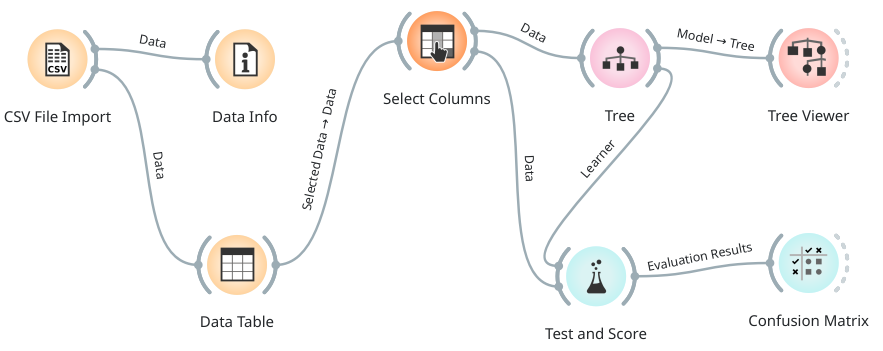
\includegraphics[width=\linewidth]{../figures/decision_tree_pipeline.png}
	\caption{Konfigurasi pipeline Orange untuk membangun decision tree dari dataset \texttt{loan.csv}}
	\label{fig:pipeline-orange}
\end{figure}




\subsection{Membangun Decision Tree dari Dataset Pinjaman}

Setelah dataset \texttt{loan.csv} dimuat dan atribut target (\texttt{loan\_approved}) ditentukan, langkah selanjutnya adalah membangun model pohon keputusan untuk memprediksi kemungkinan persetujuan pinjaman oleh lembaga keuangan. Decision tree dipilih karena model ini bersifat transparan, mudah dipahami, dan dapat divisualisasikan secara hierarkis, sehingga sangat cocok untuk kebutuhan analisis manajerial dalam dunia keuangan \cite{camm2020business}.

Di dalam Orange, pembangunan decision tree dilakukan melalui komponen \texttt{Tree}. Komponen ini secara otomatis menghasilkan model klasifikasi berdasarkan variabel input yang telah ditentukan. Prosesnya meliputi:

\begin{enumerate}
	\item \textbf{Pemilihan Atribut Pemisah (Splitting Criteria):} Orange secara default menggunakan \textit{Information Gain} atau \textit{Gini Index} untuk menentukan atribut terbaik di setiap node. Atribut ini menjadi dasar pemisahan data yang paling informatif terhadap variabel target.
	
	\item \textbf{Pembuatan Struktur Pohon:} Setelah atribut terbaik ditemukan, data dibagi ke dalam cabang-cabang berdasarkan nilai atribut tersebut. Proses ini berlanjut secara rekursif hingga pohon selesai terbentuk atau mencapai batasan tertentu, seperti kedalaman maksimum.
	
	\item \textbf{Pengendalian Overfitting:} Untuk menghindari kompleksitas model yang berlebihan, Orange menyediakan pengaturan seperti pembatasan kedalaman maksimum (\texttt{Max depth}), jumlah minimum data per simpul, dan metode pruning. Pengaturan ini dapat disesuaikan untuk menjaga keseimbangan antara akurasi dan interpretabilitas.
\end{enumerate}

Dalam praktik ini, mahasiswa disarankan untuk:

\begin{itemize}
	\item Membandingkan model pohon dengan kedalaman yang berbeda untuk memahami hubungan antara kompleksitas model dan kemudahan interpretasi.
	\item Mengamati simpul keputusan utama (root node) dan mendiskusikan alasan atribut tersebut dipilih sebagai pemisah awal.
	\item Mengevaluasi simpul daun (leaf nodes) untuk mengenali kombinasi karakteristik nasabah yang mengarah pada persetujuan (\texttt{Yes}) atau penolakan (\texttt{No}) pinjaman.
\end{itemize}

Sebagai contoh, model dapat menunjukkan bahwa nasabah dengan status pekerjaan \texttt{Employed}, tingkat pendapatan \texttt{Medium}, skor kredit \texttt{Good}, dan memiliki jaminan (\texttt{has\_collateral = True}) cenderung lebih mungkin mendapatkan persetujuan pinjaman. Pola semacam ini dapat dijadikan dasar untuk menyusun kebijakan pemberian kredit yang lebih efisien dan berbasis data.

Melalui eksplorasi visual di Orange, mahasiswa dapat memahami bagaimana pohon keputusan bekerja serta bagaimana pola-pola dalam data nasabah diterjemahkan menjadi logika bisnis yang dapat diterapkan secara nyata \cite{demsar2013orange}. 

\subsection{Visualisasi, Interpretasi Hasil, dan Insight Bisnis}

Salah satu keunggulan utama dari decision tree adalah kemampuannya untuk divisualisasikan dalam bentuk diagram pohon yang mudah dibaca. Dalam Orange, hasil pemodelan decision tree dapat ditampilkan secara interaktif melalui komponen \texttt{Tree Viewer}, yang memperlihatkan struktur node dan cabang berdasarkan pembagian data pada setiap atribut. Hal ini memudahkan manajer dan analis non-teknis untuk memahami logika di balik klasifikasi yang dihasilkan \cite{camm2020business}.

Setiap simpul dalam pohon menunjukkan kondisi yang digunakan untuk membagi data, seperti:
\begin{itemize}
	\item \texttt{credit\_score = Good}
	\item \texttt{has\_collateral = True}
	\item \texttt{income\_level = Medium}
\end{itemize}
dan setiap cabang menunjukkan kemungkinan hasil berdasarkan kondisi tersebut. Simpul daun (leaf node) akan berisi prediksi akhir (\texttt{Yes} atau \texttt{No}), jumlah observasi yang masuk ke simpul tersebut, serta persentase distribusi kelas berdasarkan data pelatihan.

Interpretasi dari hasil ini dapat membantu mahasiswa menjawab pertanyaan strategis, seperti:
\begin{itemize}
	\item Profil nasabah seperti apa yang paling mungkin disetujui pengajuan pinjamannya?
	\item Atribut mana yang paling menentukan keputusan persetujuan kredit?
	\item Bagaimana alur logika model dapat mendukung kebijakan pinjaman yang berbasis segmentasi risiko?
\end{itemize}

Sebagai contoh, hasil visualisasi dapat menunjukkan bahwa nasabah yang:
\begin{enumerate}
	\item memiliki skor kredit \texttt{Good},
	\item memiliki jaminan (\texttt{has\_collateral = True}), dan
	\item bekerja sebagai \texttt{Employed},
\end{enumerate}
memiliki probabilitas tinggi untuk mendapatkan persetujuan pinjaman. Struktur pohon keputusan yang dihasilkan dari dataset \texttt{loan.csv} ditampilkan pada Gambar~\ref{fig:loan-tree}.

\begin{figure}[h]
	\centering
	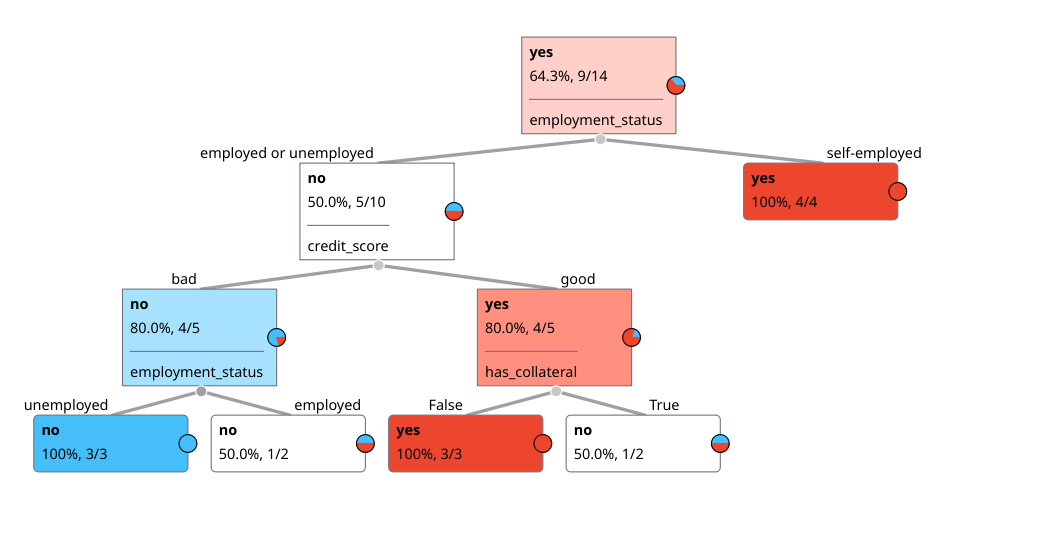
\includegraphics[width=\linewidth]{../figures/loan_tree.png}
	\caption{Visualisasi pohon keputusan hasil pemodelan dari dataset \texttt{loan.csv} di Orange}
	\label{fig:loan-tree}
\end{figure}

Insight dari model ini dapat dimanfaatkan oleh manajer risiko dan analis kredit untuk:
\begin{itemize}
	\item memprioritaskan aplikasi dari segmen berisiko rendah,
	\item menyusun kriteria kelayakan pinjaman yang lebih akurat, serta
	\item meningkatkan efisiensi dalam proses evaluasi kredit.
\end{itemize}

Visualisasi pohon keputusan juga memfasilitasi pendekatan \textit{what-if analysis}, di mana pengguna dapat menelusuri bagaimana perubahan pada atribut tertentu (misalnya, status pekerjaan atau keberadaan jaminan) dapat mengubah hasil prediksi. Ini menjadi sarana pembelajaran eksploratif yang sangat bermanfaat bagi mahasiswa manajemen yang sedang mempelajari konsep dasar analisis prediktif dan pengambilan keputusan berbasis data \cite{demsar2013orange}.

Dengan demikian, decision tree tidak hanya memberikan akurasi prediksi, tetapi juga mendukung penyusunan strategi bisnis yang lebih berbasis fakta, terukur, dan dapat dikomunikasikan secara lintas fungsi dalam organisasi.


\subsection{Eksplorasi Skema What-If dan Segmentasi Nasabah}

Salah satu keunggulan utama dari decision tree dalam konteks manajerial adalah kemampuannya untuk digunakan dalam eksplorasi skenario “what-if”. Pendekatan ini memungkinkan pengguna untuk mengevaluasi bagaimana perubahan nilai pada satu atau lebih atribut dapat memengaruhi hasil prediksi. Dalam Orange, mahasiswa dapat secara visual mengikuti jalur dalam pohon keputusan dan mengganti nilai atribut untuk melihat dampaknya terhadap keputusan akhir \cite{demsar2013orange}.

Sebagai contoh, jika seorang calon peminjam awalnya memiliki atribut:
\begin{itemize}
	\item \texttt{employment\_status = Unemployed},
	\item \texttt{credit\_score = Bad},
	\item \texttt{has\_collateral = False},
\end{itemize}
dan hasil prediksi menunjukkan \texttt{loan\_approved = No}, maka mahasiswa dapat mengganti nilai atribut menjadi:
\begin{itemize}
	\item \texttt{employment\_status = Employed},
	\item \texttt{credit\_score = Good},
	\item \texttt{has\_collateral = True},
\end{itemize}
untuk mengevaluasi apakah keputusan model berubah menjadi \texttt{loan\_approved = Yes}. Analisis seperti ini memberikan pemahaman mendalam tentang pengaruh relatif dari setiap atribut, serta dapat digunakan untuk menyusun kebijakan penyaringan kredit yang lebih adaptif.

Selain itu, decision tree juga secara alami menghasilkan \textbf{segmentasi nasabah} yang terstruktur. Setiap jalur dari root ke simpul daun dalam pohon merepresentasikan satu segmen dengan karakteristik unik. Misalnya, sebuah simpul daun mungkin berisi informasi seperti:

\begin{quote}
	“Nasabah dengan \texttt{employment\_status = Employed}, \texttt{income\_level = Medium}, \texttt{credit\_score = Good}, dan \texttt{has\_collateral = True} memiliki probabilitas tinggi untuk disetujui pinjamannya.”
\end{quote}

Segmentasi ini dapat dimanfaatkan oleh tim kredit atau manajemen risiko untuk:
\begin{enumerate}
	\item Menyusun kebijakan pinjaman yang lebih terarah berdasarkan profil peminjam yang berpotensi disetujui.
	\item Menyesuaikan persyaratan kredit dan skema bunga sesuai dengan karakteristik segmen tertentu.
	\item Melakukan prioritisasi pemrosesan aplikasi berdasarkan risiko dan potensi pengembalian.
\end{enumerate}

Pendekatan ini mendukung konsep \textit{data-driven segmentation}, di mana pengelompokan nasabah tidak hanya didasarkan pada intuisi, tetapi pada bukti empiris yang terstruktur dari hasil analitik. Dengan demikian, decision tree tidak hanya bertindak sebagai alat prediksi, tetapi juga sebagai alat eksplorasi strategi dan penyusunan kebijakan bisnis yang lebih presisi dan efektif \cite{camm2020business}.

Melalui eksplorasi skenario dan segmentasi ini, mahasiswa diharapkan mampu mengembangkan wawasan kritis dalam menyusun kebijakan keuangan atau layanan pelanggan yang responsif terhadap karakteristik dan perilaku peminjam yang berbeda-beda.



\section{Evaluasi Model dan Ukuran Kinerja}

Evaluasi model merupakan tahap krusial dalam supervised learning karena membantu menentukan apakah model yang dibangun mampu memberikan prediksi yang akurat dan relevan secara bisnis. Dalam konteks prediksi persetujuan pinjaman seperti pada praktik dengan Orange, evaluasi ini sangat penting untuk memastikan bahwa keputusan yang diambil berdasarkan model akan memberikan dampak positif terhadap efektivitas strategi kredit.

Orange menyediakan berbagai metrik evaluasi melalui komponen \texttt{Test \& Score}, yang dapat dihubungkan langsung ke model decision tree dan dataset. Komponen ini menghitung ukuran-ukuran kinerja utama seperti \textbf{accuracy}, \textbf{precision}, \textbf{recall}, dan \textbf{F1-score}, serta menyajikan ringkasan hasil dalam format tabel sederhana yang mudah dipahami. Berikut adalah penjelasan dari masing-masing metrik dan relevansinya dalam konteks bisnis:

\subsection*{1. Akurasi (Accuracy)}

Akurasi menunjukkan proporsi keseluruhan prediksi yang benar dibandingkan dengan total data. Misalnya, jika model memproses 100 data pengajuan pinjaman dan menghasilkan 85 prediksi yang sesuai dengan kenyataan, maka akurasinya adalah 85\%.

\textbf{Kelebihan:} Mudah dihitung dan dipahami.  
\textbf{Kekurangan:} Bisa menyesatkan jika distribusi kelas tidak seimbang, misalnya jika sebagian besar aplikasi pinjaman memang disetujui.

\subsection*{2. Precision}

Precision mengukur ketepatan model dalam memprediksi persetujuan pinjaman. Ini menunjukkan berapa banyak dari seluruh prediksi \texttt{Yes} (disetujui) yang memang benar-benar disetujui dalam kenyataannya.

\[
\text{Precision} = \frac{\text{True Positives}}{\text{True Positives + False Positives}}
\]

\textbf{Contoh:} Jika model memprediksi 40 pengajuan akan disetujui, tetapi hanya 30 yang benar-benar disetujui, maka precision = 75\%.

\textbf{Konteks bisnis:} Precision tinggi berarti lembaga keuangan tidak terlalu banyak menyetujui pinjaman untuk peminjam yang sebenarnya berisiko.

\subsection*{3. Recall (Sensitivity)}

Recall menunjukkan seberapa baik model dalam menemukan semua kasus persetujuan pinjaman yang seharusnya disetujui. Ini mengukur kemampuan model menangkap seluruh data positif yang benar.

\[
\text{Recall} = \frac{\text{True Positives}}{\text{True Positives + False Negatives}}
\]

\textbf{Contoh:} Jika ada 50 pengajuan yang seharusnya disetujui, dan model hanya berhasil menangkap 30, maka recall = 60\%.

\textbf{Konteks bisnis:} Recall tinggi penting untuk memastikan lembaga tidak kehilangan peluang dari nasabah yang sebenarnya layak menerima pinjaman.

\subsection*{4. F1-Score}

F1-score adalah ukuran keseimbangan antara precision dan recall, menggunakan rata-rata harmonis dari keduanya. Metode ini digunakan ketika kedua aspek—ketepatan dan kelengkapan—sama pentingnya.

\[
\text{F1-Score} = 2 \times \frac{\text{Precision} \times \text{Recall}}{\text{Precision} + \text{Recall}}
\]

\textbf{Konteks bisnis:} F1-score menjadi pilihan utama ketika lembaga ingin menghindari terlalu banyak kesalahan prediksi dalam dua arah: menyetujui pinjaman yang seharusnya ditolak, dan menolak pinjaman yang seharusnya disetujui.

\subsection*{Pemilihan Metrik Berdasarkan Tujuan Analisis}

Tidak ada satu metrik yang selalu paling cocok dalam semua situasi. Pemilihan metrik harus disesuaikan dengan strategi dan konteks bisnis:

\begin{itemize}
	\item Jika \textbf{risiko kredit macet sangat tinggi}, maka precision lebih diutamakan untuk menghindari persetujuan kepada peminjam yang tidak layak.
	\item Jika \textbf{lembaga ingin meningkatkan inklusi keuangan}, recall menjadi penting agar tidak banyak peminjam yang layak justru ditolak.
	\item Jika ingin \textbf{menyeimbangkan kedua risiko tersebut}, maka F1-score digunakan untuk memberikan gambaran performa yang lebih proporsional.
\end{itemize}

Melalui pendekatan ini, mahasiswa tidak hanya memahami angka-angka dari hasil evaluasi model, tetapi juga bagaimana mengaitkan metrik tersebut dengan dampaknya terhadap strategi dan kebijakan bisnis. Orange menyediakan platform evaluasi yang ramah pengguna sehingga proses penilaian performa model dapat dilakukan secara visual, iteratif, dan intuitif tanpa memerlukan pemrograman.

\section{Evaluasi Praktik Hands-On}

\begin{figure}[h]
	\centering
	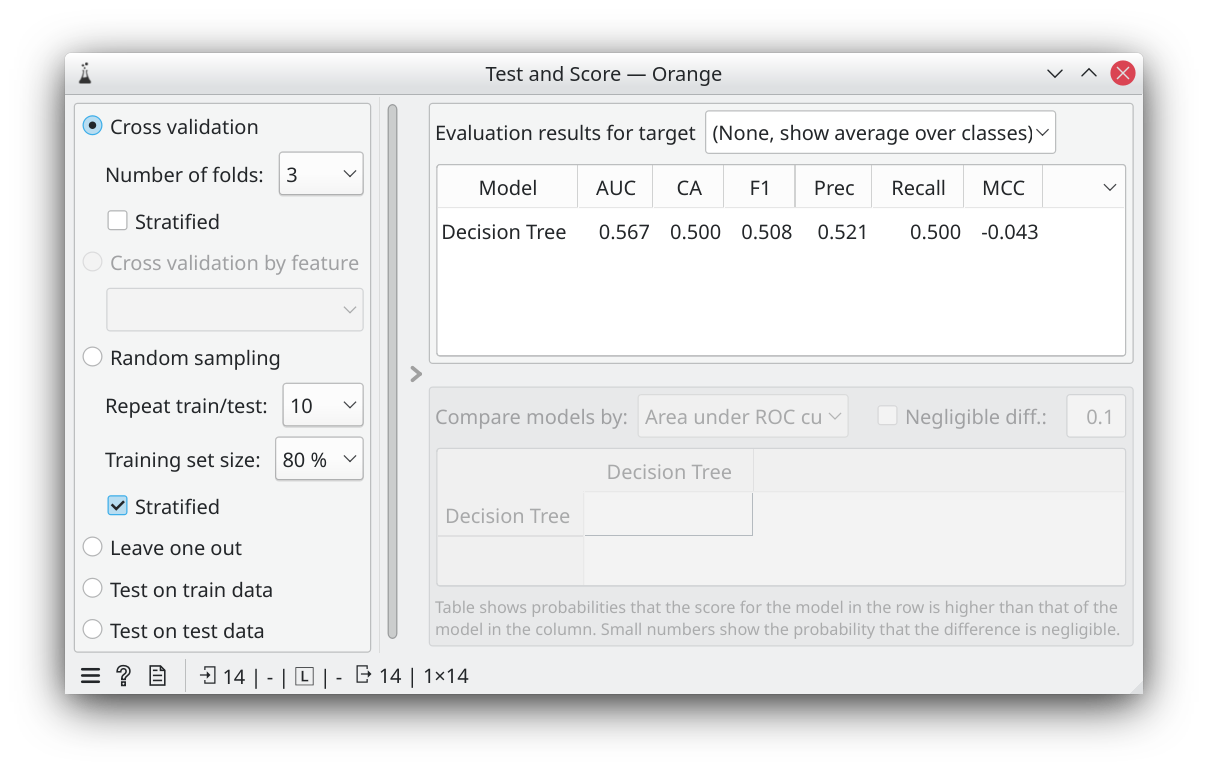
\includegraphics[width=0.9\linewidth]{../figures/decision_tree_results.png}
	\caption{Hasil evaluasi model Decision Tree pada Orange.}
\end{figure}

Evaluasi dilakukan menggunakan perangkat lunak \textit{Orange} untuk menilai kinerja model \textit{Decision Tree} terhadap dataset klasifikasi. Evaluasi dilakukan melalui widget \textit{Test and Score} dengan konfigurasi sebagai berikut:

\begin{itemize}
	\item \textbf{Metode evaluasi:} Cross Validation
	\item \textbf{Jumlah fold:} 3 (3-Fold Cross Validation)
	\item \textbf{Stratified:} Dicentang (Stratified)
	\item \textbf{Model:} Decision Tree
\end{itemize}

\textbf{Cross Validation} adalah teknik evaluasi di mana dataset dibagi menjadi beberapa bagian yang disebut \textit{fold}. Dalam konfigurasi 3-fold, data dibagi menjadi tiga bagian yang seimbang. Setiap fold secara bergiliran digunakan sebagai data uji, sementara dua fold lainnya digunakan sebagai data latih. Proses ini dilakukan sebanyak tiga kali, dan hasil evaluasi dirata-ratakan.

\textbf{Stratified Cross Validation} berarti bahwa distribusi kelas (label) dalam setiap fold dibuat serupa dengan distribusi asli pada dataset. Ini penting untuk menghindari ketimpangan kelas di salah satu fold, terutama pada data klasifikasi dengan distribusi tidak seimbang.

\subsection*{Hasil Evaluasi}

Berikut adalah nilai-nilai metrik yang dihasilkan dari proses evaluasi model Decision Tree:

\begin{center}
	\begin{tabular}{|l|c|}
		\hline
		\textbf{Metrik} & \textbf{Nilai} \\
		\hline
		AUC (Area Under Curve) & 0.567 \\
		CA (Classification Accuracy) & 0.500 \\
		F1 Score & 0.508 \\
		Precision & 0.521 \\
		Recall & 0.500 \\
		MCC (Matthews Correlation Coefficient) & -0.043 \\
		\hline
	\end{tabular}
\end{center}

\subsection*{Interpretasi Hasil Evaluasi}

\begin{itemize}
	\item \textbf{AUC (Area Under Curve)} mengukur kemampuan model untuk membedakan antar kelas. Nilai 0.567 sedikit di atas nilai acak (0.5), artinya model memiliki kemampuan terbatas untuk membedakan kelas target.
	
	\item \textbf{Classification Accuracy (CA)} sebesar 0.500 menunjukkan bahwa hanya 50\% dari seluruh prediksi model yang sesuai dengan label sebenarnya. Ini berarti model hanya benar separuh waktu.
	
	\item \textbf{F1 Score} adalah rata-rata harmonis antara precision dan recall. Nilai 0.508 menunjukkan bahwa performa model cukup seimbang antara kemampuan mengenali kelas positif dan ketepatan dalam prediksi, tetapi masih berada di level sedang.
	
	\item \textbf{Precision} sebesar 0.521 berarti dari semua prediksi positif yang diberikan oleh model, sekitar 52.1\% di antaranya benar-benar positif.
	
	\item \textbf{Recall} sebesar 0.500 berarti bahwa model berhasil mengenali 50\% dari seluruh data yang seharusnya berlabel positif.
	
	\item \textbf{Matthews Correlation Coefficient (MCC)} sebesar -0.043 menunjukkan hampir tidak ada korelasi antara hasil prediksi model dan label sebenarnya. Nilai mendekati nol mengindikasikan bahwa model belum menunjukkan performa klasifikasi yang baik.
\end{itemize}

\subsection*{Kesimpulan Sementara}

Meskipun hasil evaluasi lebih baik dibandingkan sebelumnya, performa model Decision Tree masih tergolong rendah. AUC yang sedikit di atas 0.5 menunjukkan bahwa model belum optimal dalam membedakan antar kelas. Kemungkinan penyebabnya adalah:

\begin{enumerate}
	\item \textbf{Kompleksitas data yang tinggi} atau pola antar fitur yang tidak cukup kuat untuk dipelajari oleh model Decision Tree.
	\item \textbf{Ukuran dataset yang terbatas} menyebabkan model belum mampu generalisasi dengan baik.
	\item \textbf{Distribusi fitur yang kurang informatif} terhadap target variabel.
\end{enumerate}


\section{Analisis Confusion Matrix}

\begin{figure}[h]
	\centering
	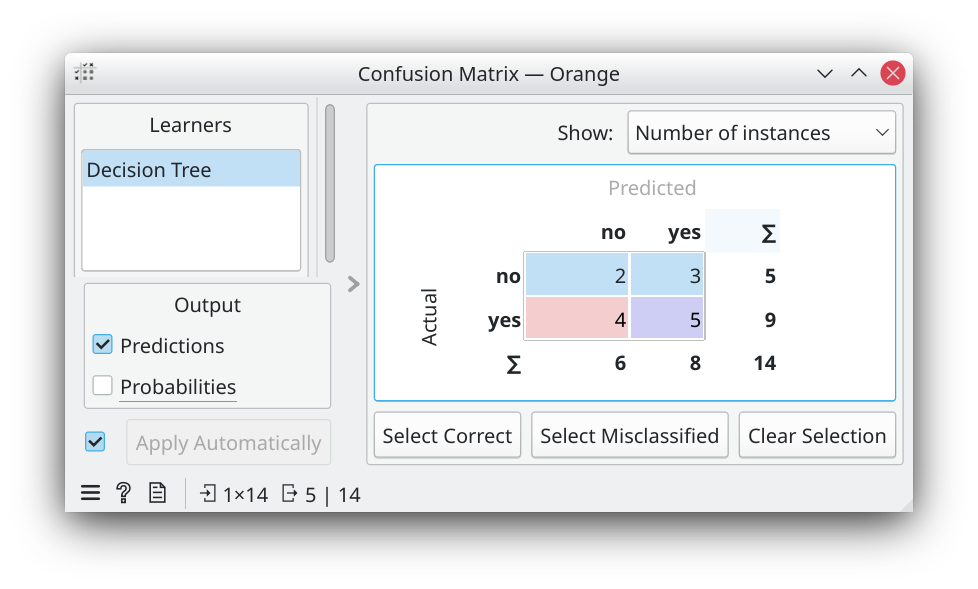
\includegraphics[width=0.7\linewidth]{../figures/decision_tree_confusion_matrix.png}
	\caption{Confusion Matrix untuk model Decision Tree pada Orange.}
\end{figure}

Confusion matrix digunakan untuk melihat secara detail performa klasifikasi berdasarkan jumlah prediksi yang benar dan salah pada masing-masing kelas. Gambar di atas menunjukkan hasil confusion matrix dari model \textit{Decision Tree} dengan dua kelas: \texttt{no} dan \texttt{yes}. 

Setiap sel dalam matriks menunjukkan jumlah instance yang diklasifikasikan pada masing-masing kombinasi kelas aktual dan kelas prediksi. Baris menyatakan label aktual, sedangkan kolom menyatakan prediksi model.

\subsection*{Isi Matriks}

\begin{center}
	\begin{tabular}{|c|c|c|c|}
		\hline
		& \textbf{Predicted: no} & \textbf{Predicted: yes} & \textbf{Total (Aktual)} \\
		\hline
		\textbf{Actual: no} & 2 (True Negative) & 3 (False Positive) & 5 \\
		\textbf{Actual: yes} & 4 (False Negative) & 5 (True Positive) & 9 \\
		\hline
		\textbf{Total (Prediksi)} & 6 & 8 & 14 \\
		\hline
	\end{tabular}
\end{center}

\subsection*{Interpretasi}

\begin{itemize}
	\item \textbf{True Positive (TP):} 5 — Kasus \texttt{yes} yang diprediksi benar sebagai \texttt{yes}.
	\item \textbf{True Negative (TN):} 2 — Kasus \texttt{no} yang diprediksi benar sebagai \texttt{no}.
	\item \textbf{False Positive (FP):} 3 — Kasus \texttt{no} yang salah diprediksi sebagai \texttt{yes}.
	\item \textbf{False Negative (FN):} 4 — Kasus \texttt{yes} yang salah diprediksi sebagai \texttt{no}.
\end{itemize}

\subsection*{Perhitungan Metrik Berdasarkan Confusion Matrix}

Dari nilai-nilai tersebut dapat dihitung ulang beberapa metrik dasar untuk validasi:

\begin{itemize}
	\item \textbf{Accuracy} = \( \frac{TP + TN}{TP + TN + FP + FN} = \frac{5 + 2}{14} = 0.500 \)
	\item \textbf{Precision} = \( \frac{TP}{TP + FP} = \frac{5}{5 + 3} = 0.625 \)
	\item \textbf{Recall} = \( \frac{TP}{TP + FN} = \frac{5}{5 + 4} = 0.556 \)
	\item \textbf{F1 Score} = \( 2 \times \frac{Precision \times Recall}{Precision + Recall} \approx 0.588 \)
\end{itemize}

Perlu dicatat bahwa nilai-nilai metrik dari confusion matrix ini dapat sedikit berbeda dari rata-rata yang ditampilkan pada hasil \textit{Test and Score}, karena confusion matrix biasanya dihitung dari agregasi keseluruhan prediksi (bukan rata-rata per fold).

\subsection*{Kesimpulan}

Model Decision Tree masih menunjukkan performa yang moderat. Dari confusion matrix terlihat bahwa model lebih sering salah dalam memprediksi kelas \texttt{yes} sebagai \texttt{no} (FN = 4), dan juga melakukan sejumlah kesalahan dalam memprediksi \texttt{no} sebagai \texttt{yes} (FP = 3). Untuk meningkatkan akurasi, disarankan eksplorasi model lain, tuning parameter, serta pemilihan fitur yang lebih relevan.


\section{Latihan Mandiri: Karakterisasi Churn Pelanggan dengan Decision Tree}

Gunakan dataset \textit{Telco Customer Churn} dari Kaggle untuk membangun model prediksi menggunakan decision tree di Orange. Dataset ini berisi data pelanggan layanan telekomunikasi dan status churn mereka (\texttt{Churn = Yes/No}).

\subsection*{Langkah Praktik}

\begin{enumerate}
	\item Kunjungi \url{https://www.kaggle.com/datasets/blastchar/telco-customer-churn}, kemudian unduh dataset.
	\item Buka Orange dan buat alur kerja (\textit{workflow}) dengan komponen. 
	\begin{itemize}
		\item \texttt{File} – untuk memuat \texttt{Telco-Customer-Churn.csv}
		\item \texttt{Select Columns} – atur \texttt{Churn} sebagai target
		\item \texttt{Data Table} – untuk melihat isi data
		\item \texttt{Tree} – untuk membangun model decision tree
	\end{itemize}
	\item Jalankan model dan amati atribut yang paling memengaruhi churn.
	\item Tampilkan hasil pohon dan simpulkan hasil analisis.
\end{enumerate}

\subsection*{Output yang Diharapkan}

\begin{itemize}
	\item Visual pohon keputusan dari Orange.
	\item Ringkasan interpretasi simpul utama.
	\item Rekomendasi singkat berdasarkan hasil model.
	\item Hasil Evaluasi
\end{itemize}


\section{Rangkuman}

Machine Learning (ML), khususnya pendekatan supervised learning, merupakan tahap lanjutan dalam strategi Big Data yang berfokus pada penciptaan nilai melalui analitik prediktif dan preskriptif. Setelah data dikumpulkan, disimpan, dan diproses, ML memungkinkan organisasi tidak hanya memahami apa yang terjadi di masa lalu (descriptive analytics), tetapi juga memprediksi apa yang akan terjadi dan merekomendasikan tindakan terbaik yang dapat diambil (prescriptive analytics) \cite{provost2013data}. Dalam konteks bisnis, ML menjadi enabler utama bagi pengambilan keputusan berbasis data, yang lebih cepat, akurat, dan relevan terhadap kondisi pasar yang dinamis.

Ke depan, organisasi dapat mengeksplorasi pendekatan lanjutan seperti AutoML (automated machine learning) untuk menyederhanakan proses pemodelan, serta mengintegrasikan hasil ML ke dalam dashboard interaktif yang mudah diinterpretasi oleh manajemen. Visualisasi hasil prediksi, pelacakan kinerja model, dan pembaruan model berbasis data baru merupakan aspek penting dalam integrasi ML dengan sistem pengambilan keputusan sehari-hari. Dengan membangun budaya data-driven dan tata kelola data yang kuat, Machine Learning dapat dioptimalkan sebagai aset strategis dalam keseluruhan arsitektur Big Data for Business.

	\chapter{Pengenalan Unsupervised Learning}

\section{Pengantar Unsupervised Learning}

\textbf{Unsupervised Learning} merupakan salah satu pendekatan utama dalam Machine Learning yang digunakan ketika data yang tersedia tidak memiliki label atau keluaran yang diketahui sebelumnya. Berbeda dengan \textit{supervised learning}, di mana model dilatih berdasarkan pasangan data input dan output, dalam \textit{unsupervised learning} model berusaha menemukan struktur, pola, atau keteraturan tersembunyi di dalam data secara mandiri tanpa panduan eksplisit \cite{hastie2009elements}.

Tujuan utama dari unsupervised learning bukanlah membuat prediksi terhadap label yang telah ditentukan, melainkan mengekstraksi representasi yang bermanfaat, melakukan segmentasi, atau mereduksi kompleksitas data agar lebih mudah dipahami dan dianalisis. Dalam konteks bisnis, pendekatan ini sangat berguna ketika organisasi memiliki banyak data historis tetapi tidak memiliki anotasi atau hasil akhir yang terstruktur secara eksplisit.

Contoh nyata dari penerapan unsupervised learning dalam dunia bisnis meliputi:
\begin{itemize}
	\item \textbf{Segmentasi pelanggan:} mengelompokkan pelanggan ke dalam segmen-segmen homogen berdasarkan perilaku pembelian, preferensi, atau demografi tanpa perlu label manual.
	\item \textbf{Deteksi anomali:} mengidentifikasi transaksi yang tidak biasa atau mencurigakan dalam sistem keuangan tanpa memerlukan contoh eksplisit dari penipuan sebelumnya.
	\item \textbf{Reduksi dimensi:} menyederhanakan data berdimensi tinggi (seperti data sensor IoT atau profil pelanggan) untuk memudahkan visualisasi dan analisis lebih lanjut.
\end{itemize}

Salah satu perbedaan mendasar antara supervised dan unsupervised learning adalah \textbf{ketersediaan label}. Pada supervised learning, model didorong untuk belajar dari hubungan antara input dan output yang telah diketahui, sedangkan pada unsupervised learning, tidak ada target output yang eksplisit. Oleh karena itu, evaluasi keberhasilan model unsupervised sering kali memerlukan pendekatan eksploratif, visualisasi, atau validasi eksternal berbasis domain bisnis.

Secara umum, unsupervised learning sangat cocok digunakan pada tahap eksplorasi awal dalam proses analitik data, terutama ketika:
\begin{itemize}
	\item Label data sulit diperoleh atau membutuhkan biaya tinggi,
	\item Tujuan analisis bersifat eksploratif, misalnya memahami struktur data,
	\item Organisasi ingin menggali pola baru atau potensi segmen yang belum diketahui.
\end{itemize}

Pendekatan ini sangat relevan dalam era Big Data, di mana data yang tersedia terus bertambah tetapi tidak selalu teranotasi secara manual. Unsupervised learning memungkinkan organisasi untuk memperoleh wawasan awal yang penting, mengelompokkan entitas yang serupa, dan mengenali outlier yang berpotensi mengindikasikan risiko atau peluang tersembunyi \cite{ghahramani2004unsupervised}.

Dengan memahami prinsip dasar unsupervised learning, pengambil keputusan dapat lebih siap untuk mengidentifikasi area bisnis yang dapat memperoleh manfaat dari segmentasi otomatis, deteksi pola tersembunyi, dan eksplorasi data yang lebih dalam sebagai landasan untuk strategi berbasis data.

\section{Clustering: Segmentasi Otomatis Tanpa Label}

\begin{figure}[h]
	\centering
	\begin{tikzpicture}[scale=1.2]
		
		% Cluster A - Red
		\fill[red!20] (0,0) circle (1);
		\foreach \x/\y in {0.1/0.3, -0.3/-0.2, 0.2/-0.5, -0.4/0.4, 0.5/0.1} {
			\fill[red] (\x,\y) circle (2pt);
		}
		\node[red!70!black] at (0, -1.2) {\small Cluster A};
		\node[red!70!black] at (0, 0) {\tiny $\times$};
		
		% Cluster B - Blue
		\fill[blue!20] (4,0.5) circle (1);
		\foreach \x/\y in {3.7/0.8, 4.1/0.2, 4.2/0.7, 3.9/1.1, 4.3/0.4} {
			\fill[blue] (\x,\y) circle (2pt);
		}
		\node[blue!70!black] at (4, -0.7) {\small Cluster B};
		\node[blue!70!black] at (4, 0.5) {\tiny $\times$};
		
		% Cluster C - Green
		\fill[green!20] (2,3) circle (1);
		\foreach \x/\y in {1.8/2.7, 2.3/3.2, 2.1/3.3, 1.7/3.1, 2.4/2.8} {
			\fill[green!60!black] (\x,\y) circle (2pt);
		}
		\node[green!50!black] at (2, 1.7) {\small Cluster C};
		\node[green!50!black] at (2, 3) {\tiny $\times$};
		
		% Axes
		\draw[->, thick] (-1.5, -1.5) -- (5.5, -1.5) node[right] {\small Feature 1};
		\draw[->, thick] (-1.5, -1.5) -- (-1.5, 4) node[above] {\small Feature 2};
		
	\end{tikzpicture}
	\caption{Illustration of clustering in 2D feature space with three distinct groups and centroids}
	\label{fig:clustering-tikz}
\end{figure}

\textbf{Clustering} merupakan salah satu teknik utama dalam unsupervised learning yang bertujuan untuk mengelompokkan data ke dalam grup atau klaster berdasarkan kemiripan (similarity) antar data (Gambar~\ref{fig:clustering-tikz}). Dalam clustering, tidak tersedia label atau kategori sebelumnya. Oleh karena itu, algoritma clustering akan secara otomatis mencari pola dan struktur tersembunyi dalam data untuk membentuk grup-grup yang saling homogen di dalam dan heterogen antar kelompok \cite{kelleher2015fundamentals}.

\subsection*{Tujuan Clustering dalam Bisnis}

Dalam konteks bisnis, clustering sangat bermanfaat untuk mendukung pengambilan keputusan berbasis segmentasi, terutama ketika organisasi tidak memiliki label eksplisit terhadap entitas dalam datanya. Beberapa tujuan utama penggunaan clustering dalam dunia bisnis antara lain:

\begin{itemize}
	\item \textbf{Segmentasi pelanggan:} mengelompokkan pelanggan berdasarkan perilaku pembelian, pola interaksi, nilai transaksi, atau demografi untuk menyusun strategi pemasaran yang lebih tepat sasaran.
	\item \textbf{Personalisasi layanan:} menyusun paket produk atau promosi yang disesuaikan dengan profil segmen pelanggan tertentu.
	\item \textbf{Identifikasi pola pemakaian produk:} mengenali kelompok pengguna berdasarkan cara mereka menggunakan layanan atau fitur tertentu.
	\item \textbf{Analisis lokasi:} mengelompokkan wilayah geografis berdasarkan potensi pasar, tingkat permintaan, atau pola distribusi.
\end{itemize}

Dengan melakukan segmentasi otomatis melalui clustering, organisasi dapat meningkatkan efisiensi kampanye pemasaran, meningkatkan kepuasan pelanggan, dan mendukung pengambilan keputusan yang berbasis data.

\subsection*{Metode Clustering Populer}

Terdapat berbagai algoritma clustering yang umum digunakan, masing-masing memiliki pendekatan berbeda dalam mengelompokkan data. Berikut adalah tiga metode yang paling banyak digunakan dalam praktik bisnis:

\paragraph{1. K-Means Clustering.} K-Means adalah algoritma clustering yang membagi data ke dalam \( k \) kelompok berdasarkan jarak rata-rata terhadap pusat klaster (\textit{centroid}). Prosesnya iteratif:
\begin{enumerate}
	\item Tentukan jumlah klaster \( k \),
	\item Inisialisasi pusat klaster secara acak,
	\item Kelompokkan setiap data ke klaster terdekat,
	\item Hitung ulang posisi pusat klaster berdasarkan data yang tergabung,
	\item Ulangi proses hingga konvergen (perubahan posisi klaster minimal).
\end{enumerate}

\textbf{Kelebihan:} cepat, sederhana, cocok untuk data besar.  
\textbf{Kekurangan:} perlu menentukan \( k \) di awal, sensitif terhadap outlier, hanya efektif untuk klaster berbentuk bulat dan ukuran seimbang.

\paragraph{2. Hierarchical Clustering.} Hierarchical clustering membentuk struktur pohon (\textit{dendrogram}) dari data dengan dua pendekatan:
\begin{itemize}
	\item \textbf{Agglomerative (bottom-up):} setiap data dianggap sebagai klaster tunggal, lalu digabung bertahap hingga menjadi satu klaster besar.
	\item \textbf{Divisive (top-down):} mulai dari satu klaster besar, lalu dipisah menjadi klaster lebih kecil secara bertahap.
\end{itemize}

\textbf{Kelebihan:} tidak perlu menentukan jumlah klaster di awal, hasil dapat divisualisasikan secara hierarkis.  
\textbf{Kekurangan:} tidak efisien untuk data besar, sulit diperbarui jika ada data baru.

\paragraph{3. DBSCAN (Density-Based Spatial Clustering of Applications with Noise).} DBSCAN mengelompokkan data berdasarkan kepadatan (density). Dua poin dianggap berada dalam satu klaster jika cukup berdekatan dan terdapat cukup banyak tetangga di sekitarnya. Algoritma ini mampu mendeteksi:
\begin{itemize}
	\item Klaster dengan bentuk arbitrer (tidak harus bulat),
	\item Titik data yang tidak termasuk klaster manapun (anomali atau noise).
\end{itemize}

\textbf{Kelebihan:} tidak perlu menentukan jumlah klaster, mampu menangani bentuk klaster yang kompleks dan mendeteksi outlier.  
\textbf{Kekurangan:} performa menurun pada data berdimensi tinggi, sensitif terhadap parameter jarak dan minimum tetangga.

\subsection*{Pemilihan Metode Clustering}

Pemilihan algoritma clustering bergantung pada:
\begin{itemize}
	\item Bentuk dan ukuran klaster yang diharapkan,
	\item Skala dan dimensi data,
	\item Tujuan analisis (misalnya segmentasi vs. deteksi anomali),
	\item Kebutuhan interpretabilitas dan visualisasi.
\end{itemize}

Dalam praktik bisnis, K-Means sering menjadi pilihan awal karena sederhana dan efisien, sedangkan DBSCAN cocok untuk mendeteksi perilaku ekstrem atau segmen kecil yang tersembunyi. Hierarchical clustering berguna dalam eksplorasi awal untuk memahami struktur segmentasi sebelum menentukan jumlah klaster yang tepat.


\section{Visualisasi dan Reduksi Dimensi}

Dalam dunia bisnis dan analitik data, sering kali kita dihadapkan pada dataset berdimensi tinggi, yaitu data dengan banyak variabel atau fitur. Contohnya adalah data pelanggan dengan ratusan atribut seperti perilaku pembelian, histori transaksi, demografi, dan interaksi digital. Dataset berdimensi tinggi dapat menyulitkan proses analisis, visualisasi, dan pembelajaran mesin. Oleh karena itu, dibutuhkan teknik \textbf{reduksi dimensi} (\textit{dimensionality reduction}) untuk menyederhanakan representasi data tanpa kehilangan informasi penting secara signifikan \cite{kelleher2015fundamentals}.

\subsection*{Mengapa Reduksi Dimensi Penting?}

Reduksi dimensi memiliki beberapa tujuan strategis dalam proses analisis data dan penerapan machine learning:

\begin{itemize}
	\item \textbf{Visualisasi:} Data berdimensi tinggi tidak dapat langsung divisualisasikan. Reduksi dimensi memungkinkan kita memetakan data ke dalam 2 atau 3 dimensi sehingga pola atau kelompok dalam data menjadi terlihat.
	
	\item \textbf{Reduksi noise:} Banyak variabel dalam data dapat mengandung noise (gangguan acak) atau redundansi (informasi berulang). Reduksi dimensi membantu menghilangkan fitur yang tidak relevan atau terlalu berkorelasi.
	
	\item \textbf{Efisiensi komputasi:} Semakin banyak fitur, semakin besar pula beban komputasi dalam pelatihan model machine learning. Reduksi dimensi mempercepat proses ini tanpa mengorbankan performa.
	
	\item \textbf{Mengatasi curse of dimensionality:} Dalam dataset berdimensi tinggi, jarak antar data menjadi kurang bermakna dan model sulit menemukan pola. Reduksi dimensi membantu menghindari fenomena ini.
\end{itemize}

\subsection*{Teknik Populer untuk Reduksi Dimensi}

Beberapa metode telah dikembangkan untuk mereduksi dimensi data. Berikut dua teknik yang paling populer dan banyak digunakan dalam analisis bisnis:

\paragraph{1. Principal Component Analysis (PCA)}

\textbf{PCA} adalah metode linier yang mengubah data asli ke dalam himpunan variabel baru yang disebut \textit{principal components}. Komponen ini merupakan kombinasi linier dari fitur-fitur asli dan disusun berdasarkan kontribusinya terhadap variasi data. Komponen pertama menjelaskan variasi terbesar, diikuti oleh komponen kedua, dan seterusnya.

\textbf{Kelebihan:}
\begin{itemize}
	\item Efisien secara komputasi,
	\item Mudah diinterpretasikan,
	\item Cocok untuk data numerik dan linier.
\end{itemize}

\textbf{Kekurangan:}
\begin{itemize}
	\item Tidak mampu menangkap pola non-linier,
	\item Hasil reduksi sulit dipetakan kembali ke fitur asli.
\end{itemize}

\textbf{Contoh bisnis:} PCA dapat digunakan untuk menyederhanakan data survei pelanggan dengan banyak pertanyaan menjadi beberapa dimensi utama seperti “kepuasan layanan”, “harga”, dan “kualitas produk”.

\paragraph{2. t-Distributed Stochastic Neighbor Embedding (t-SNE)}

\textbf{t-SNE} adalah metode non-linier yang sangat populer untuk \textbf{visualisasi data}. Teknik ini memetakan data berdimensi tinggi ke dalam dua atau tiga dimensi dengan mempertahankan hubungan lokal antar data — artinya, data yang serupa akan dipetakan berdekatan di ruang 2D/3D.

\textbf{Kelebihan:}
\begin{itemize}
	\item Sangat efektif untuk visualisasi klaster atau segmen,
	\item Mampu menangkap struktur kompleks yang tidak linier.
\end{itemize}

\textbf{Kekurangan:}
\begin{itemize}
	\item Tidak cocok untuk pemrosesan data skala besar (mahal secara komputasi),
	\item Tidak cocok sebagai tahap preprocessing sebelum supervised learning,
	\item Hasil visual tidak selalu konsisten jika dijalankan ulang.
\end{itemize}

\textbf{Contoh bisnis:} t-SNE banyak digunakan untuk memvisualisasikan hasil segmentasi pelanggan, sehingga manajer dapat memahami secara intuitif pengelompokan dan relasi antar kelompok pelanggan.

\subsection*{Perbandingan Singkat PCA dan t-SNE}

\begin{center}
	\begin{tabular}{|l|c|c|}
		\hline
		\textbf{Kriteria} & \textbf{PCA} & \textbf{t-SNE} \\
		\hline
		Jenis Algoritma & Linier & Non-linier \\
		Tujuan utama & Reduksi dimensi & Visualisasi klaster \\
		Output utama & Komponen utama & Peta 2D atau 3D \\
		Skalabilitas & Tinggi & Terbatas \\
		Hasil dapat direproduksi & Ya & Tidak selalu \\
		Dapat digunakan untuk training model & Ya & Tidak disarankan \\
		\hline
	\end{tabular}
\end{center}


Reduksi dimensi adalah langkah penting dalam proses analisis data modern, terutama dalam unsupervised learning. Teknik seperti PCA dan t-SNE tidak hanya membantu dalam visualisasi hasil segmentasi, tetapi juga meningkatkan efisiensi dan efektivitas dalam pemrosesan data besar. Dalam konteks bisnis, penggunaan reduksi dimensi memungkinkan pengambil keputusan untuk lebih cepat memahami struktur data yang kompleks dan membentuk strategi yang lebih tajam berdasarkan representasi visual dan analitis yang disederhanakan.


\section{Penerapan Clustering untuk Segmentasi Pelanggan}

Segmentasi pelanggan adalah salah satu penerapan paling umum dari teknik \textit{clustering} dalam dunia bisnis. Tujuan utamanya adalah membagi pelanggan ke dalam beberapa kelompok atau segmen berdasarkan kesamaan karakteristik atau perilaku, sehingga strategi pemasaran dan layanan dapat disesuaikan dengan kebutuhan spesifik tiap kelompok \cite{williams2020data}.

Pendekatan ini sangat berguna bagi perusahaan yang memiliki basis pelanggan besar dan heterogen, di mana perlakuan seragam terhadap semua pelanggan sering kali tidak efektif. Dengan mengenali kelompok pelanggan secara otomatis melalui clustering, perusahaan dapat mengembangkan strategi yang lebih personal, relevan, dan efisien.

\subsection*{Studi Kasus: Segmentasi Pelanggan Toko Online}

Dalam contoh ini, sebuah toko online ingin memahami segmentasi pelanggannya berdasarkan data transaksi historis. Dataset yang digunakan mencakup ribuan pelanggan dan mencatat informasi seperti:

\begin{itemize}
	\item \textbf{Frekuensi pembelian:} jumlah transaksi dalam periode tertentu.
	\item \textbf{Monetary value:} total nilai transaksi (dalam satuan mata uang).
	\item \textbf{Recency:} jumlah hari sejak transaksi terakhir.
	\item \textbf{Kategori produk:} ragam jenis produk yang dibeli.
	\item \textbf{Metode pembayaran:} misalnya transfer, kartu kredit, e-wallet.
\end{itemize}

Untuk analisis awal, dilakukan pemilihan fitur utama menggunakan pendekatan RFM (Recency, Frequency, Monetary) karena telah terbukti efektif dalam analisis perilaku pelanggan. Data kemudian dinormalisasi untuk menghindari bias terhadap fitur dengan skala besar.

\subsection*{Proses Clustering dan Hasilnya}

Setelah data siap, dilakukan \textbf{K-Means Clustering} dengan asumsi awal \( k = 4 \) klaster. Jumlah klaster ditentukan menggunakan metode \textit{elbow} untuk memastikan keseimbangan antara kompleksitas dan akurasi pengelompokan.

\textbf{Hasil clustering} menunjukkan empat kelompok pelanggan utama sebagai berikut:

\begin{enumerate}
	\item \textbf{Klaster A – Pelanggan Loyal:} frekuensi tinggi, nilai transaksi tinggi, dan recency rendah. Segmen ini adalah pelanggan paling aktif dan setia. Cocok untuk program loyalitas atau VIP.
	
	\item \textbf{Klaster B – Pelanggan Potensial:} frekuensi dan nilai transaksi sedang, namun dengan recency rendah. Mereka baru-baru ini bertransaksi, sehingga berpotensi dikembangkan menjadi pelanggan loyal.
	
	\item \textbf{Klaster C – Pelanggan Pasif:} frekuensi rendah, nilai transaksi rendah, dan recency tinggi. Mereka jarang melakukan pembelian dan terakhir bertransaksi sudah lama. Strategi reaktivasi dapat digunakan untuk segmen ini.
	
	\item \textbf{Klaster D – Pelanggan Sensitif Harga:} frekuensi cukup sering namun dengan nilai transaksi rendah. Mereka cenderung melakukan pembelian kecil dan mungkin hanya tertarik pada promosi. Cocok untuk kampanye diskon atau bundling.
\end{enumerate}

\subsection*{Manfaat Bisnis dari Segmentasi}

Dengan hasil klaster di atas, perusahaan dapat menyusun strategi yang lebih terfokus:

\begin{itemize}
	\item Menawarkan \textbf{insentif eksklusif} bagi pelanggan loyal untuk menjaga retensi.
	\item Mengembangkan \textbf{email campaign bertarget} untuk mengajak pelanggan pasif kembali.
	\item Merancang \textbf{paket diskon atau promo} untuk pelanggan sensitif harga.
	\item Meluncurkan \textbf{program onboarding} bagi pelanggan baru dalam klaster potensial.
\end{itemize}

Pendekatan ini juga membantu dalam alokasi anggaran pemasaran secara lebih efisien, karena setiap segmen memiliki kebutuhan dan perilaku yang berbeda. Selain itu, hasil clustering dapat digunakan sebagai masukan dalam sistem rekomendasi, analisis churn, dan strategi penetapan harga.

\subsection*{Visualisasi dan Evaluasi}

Setelah klaster terbentuk, visualisasi menggunakan \textbf{PCA} atau \textbf{t-SNE} dapat dilakukan untuk memetakan pelanggan dalam ruang dua dimensi. Hal ini memudahkan manajer untuk melihat distribusi dan kedekatan antar klaster. Warna yang berbeda dapat digunakan untuk menandai klaster, dan ciri khas tiap kelompok dapat dianalisis dengan melihat distribusi fitur utama di masing-masing segmen.

Meskipun clustering adalah metode eksploratif, evaluasi dapat dilakukan dengan menggunakan \textbf{silhouette score} atau \textbf{Davies-Bouldin Index} untuk mengukur seberapa baik pemisahan antar klaster dan kepadatan dalam klaster.

Melalui penerapan clustering untuk segmentasi pelanggan, perusahaan dapat lebih memahami perilaku konsumennya dan membangun strategi yang tidak hanya berdasarkan intuisi, tetapi juga berdasarkan struktur data yang konkret dan terukur.


\section{Hands-On Orange: Segmentasi Pelanggan dengan K-Means}

Orange adalah perangkat lunak visualisasi dan analisis data berbasis komponen yang sangat cocok untuk pembelajaran konsep machine learning secara praktis dan intuitif. Salah satu keunggulan Orange adalah kemampuannya untuk membangun alur kerja (\textit{workflow}) melalui antarmuka drag-and-drop, tanpa perlu menulis kode. Pada bagian ini, akan dijelaskan langkah-langkah praktis untuk menerapkan \textbf{K-Means Clustering} dalam kasus segmentasi pelanggan menggunakan Orange.

\subsection*{Tujuan Praktikum}

Tujuan dari sesi hands-on ini adalah untuk membagi pelanggan ke dalam beberapa segmen berdasarkan perilaku atau atribut tertentu, menggunakan algoritma K-Means. Setelah segmentasi berhasil dilakukan, hasilnya akan divisualisasikan dan dianalisis untuk melihat pola kelompok yang terbentuk.

\subsection*{Dataset}

Untuk praktikum ini digunakan dataset pelanggan dalam format CSV (Comma Separated Values) dengan beberapa fitur utama, antara lain:

\begin{itemize}
	\item \textbf{Recency}: jumlah hari sejak transaksi terakhir.
	\item \textbf{Frequency}: jumlah transaksi yang dilakukan.
	\item \textbf{Monetary}: total nilai pembelian.
	\item \textbf{Customer ID}: identifikasi unik pelanggan (tidak digunakan untuk clustering).
\end{itemize}

Dataset ini tersedia secara publik dan dapat diunduh melalui tautan berikut:

\begin{itemize}
	\item \textbf{UCI Machine Learning Repository}: \url{https://archive.ics.uci.edu/ml/datasets/Online+Retail}
	\item \textbf{Versi RFM siap pakai/}:\\ \url{https://u.pcloud.link/publink/show?code=kZ6a7W5Zr4Y3H3bMCSfxrMGxSut20VEohrGk} dengan nama file \texttt{frm\_results.csv}.
\texttt{}\end{itemize}

Pastikan dataset sudah tersedia secara lokal sebelum memulai proses dan disimpan dalam format \texttt{.csv} agar dapat langsung dibaca oleh komponen \texttt{File} di Orange.


\subsection*{Langkah-langkah Penyusunan Workflow}

\begin{figure}[h]
	\centering
	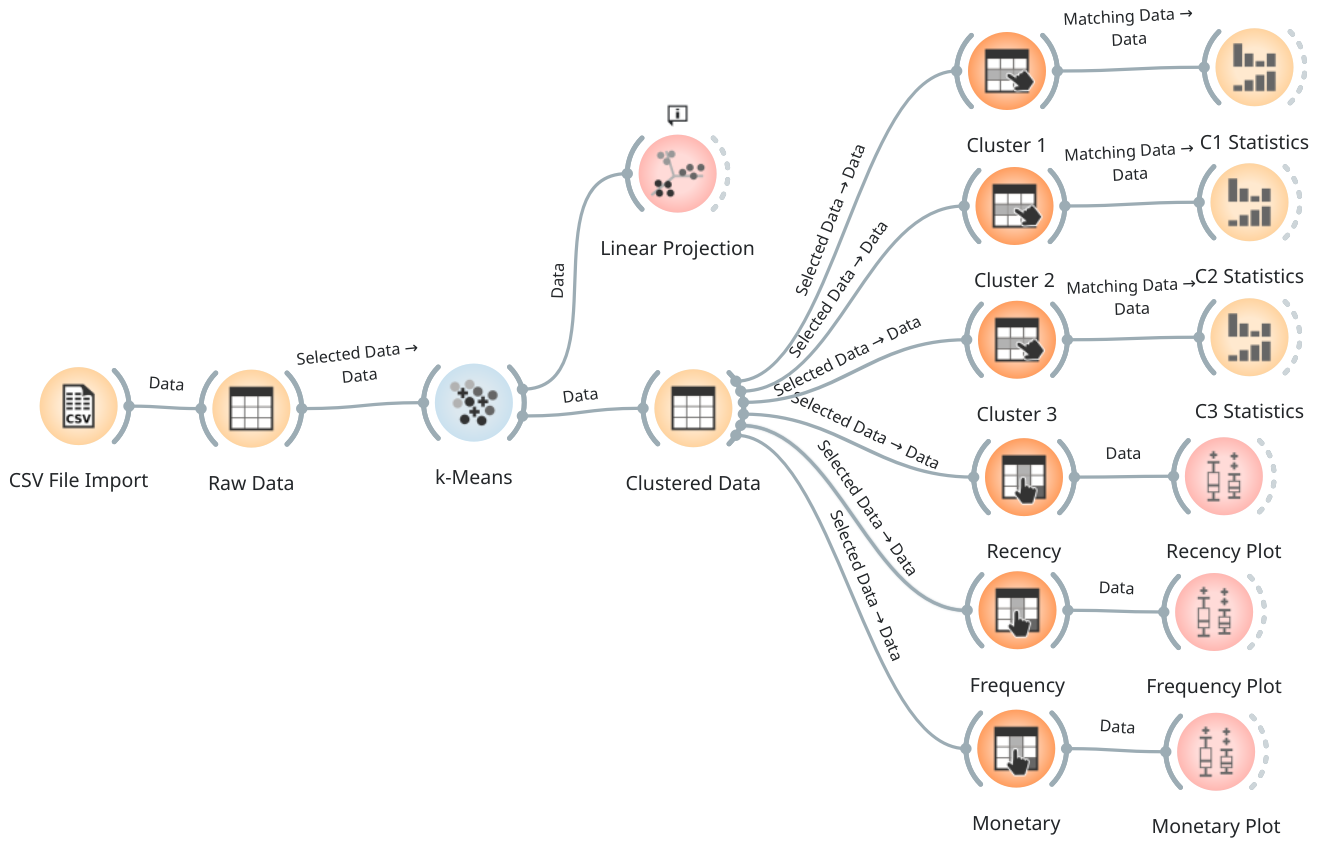
\includegraphics[width=\linewidth]{../figures/clustering.png}
	\caption{Segmentasi pelanggan menggunakan algoritma clustering K-Means}
	\label{fig:clustering-orange}
\end{figure}

Gambar \ref{fig:clustering-orange} menunjukkan alur lengkap untuk melakukan segmentasi pelanggan dengan algoritma K-Means di Orange. Langkah-langkah penyusunan workflow adalah sebagai berikut:

\begin{enumerate}
	\item \textbf{CSV File Import}: Mulai dengan mengimpor dataset menggunakan widget \texttt{File}, lalu arahkan ke file \texttt{frm\_results.csv}.
	\item \textbf{Raw Data}: Data mentah yang diimpor akan ditampilkan pada widget \texttt{Data Table} untuk verifikasi dan pemilihan fitur.
	\item \textbf{k-Means}: Hubungkan data ke widget \texttt{k-Means} untuk melakukan proses clustering. Pilih jumlah klaster yang diinginkan (misalnya 3).
	\item \textbf{Clustered Data}: Output dari \texttt{k-Means} akan diteruskan ke widget \texttt{Data Table} untuk melihat hasil klasterisasi.
	\item \textbf{Linear Projection}: Gunakan \texttt{Linear Projection} untuk memvisualisasikan hasil clustering dalam bentuk dua dimensi (scatter plot).
	\item \textbf{Cluster Statistics}: Bagi hasil klaster menjadi beberapa subset (misalnya \texttt{Cluster 1}, \texttt{Cluster 2}, \texttt{Cluster 3}), kemudian analisis masing-masing menggunakan widget \texttt{Statistics}.
	\item \textbf{RFM Plotting}: Pisahkan data berdasarkan atribut \texttt{Recency}, \texttt{Frequency}, dan \texttt{Monetary}, kemudian gunakan widget \texttt{Box Plot} untuk masing-masing atribut guna memahami distribusi nilai dalam tiap klaster.
\end{enumerate}

\begin{figure}[h]
	\centering
	\begin{subfigure}[t]{0.48\textwidth}
		\centering
		\fbox{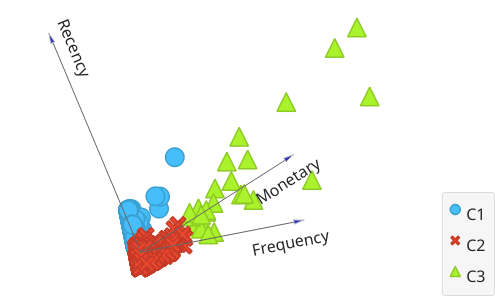
\includegraphics[width=\linewidth]{../figures/3d_plot.png}}
		\caption{Cluster in 3D (RFM space)}
	\end{subfigure}
	\hfill
	\begin{subfigure}[t]{0.48\textwidth}
		\centering
		\fbox{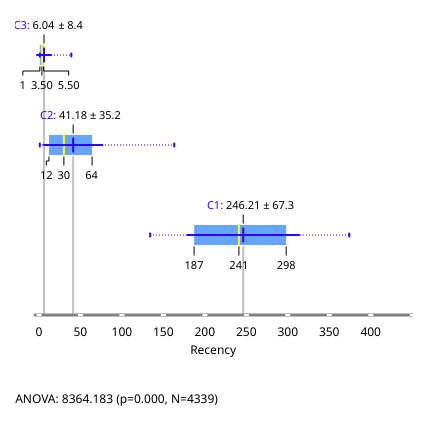
\includegraphics[width=\linewidth]{../figures/recency.png}}
		\caption{Recency Distribution}
	\end{subfigure}
	
	\vspace{10pt}
	
	\begin{subfigure}[t]{0.48\textwidth}
		\centering
		\fbox{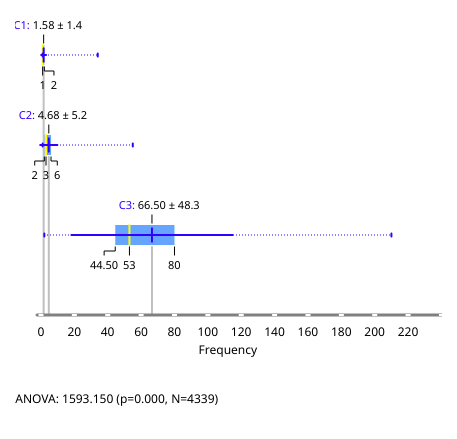
\includegraphics[width=\linewidth]{../figures/frequency.png}}
		\caption{Frequency Distribution}
	\end{subfigure}
	\hfill
	\begin{subfigure}[t]{0.48\textwidth}
		\centering
		\fbox{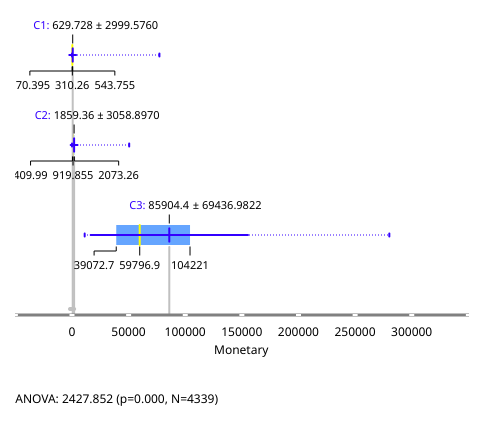
\includegraphics[width=\linewidth]{../figures/monetary.png}}
		\caption{Monetary Distribution}
	\end{subfigure}
	
	\caption{Customer segmentation results using K-Means: cluster layout and RFM distribution}
	\label{fig:clustering-subfigures}
\end{figure}


\subsection*{Analisis Hasil}

Setelah workflow selesai, hasil clustering dapat dianalisis sebagai berikut:

\begin{itemize}
	\item Amati ukuran masing-masing klaster (jumlah pelanggan dalam tiap segmen).
	\item Identifikasi karakteristik khas setiap klaster, misalnya:
	\begin{itemize}
		\item Klaster dengan \texttt{Monetary} tinggi $\rightarrow$ pelanggan VIP.
		\item Klaster dengan \texttt{Recency} tinggi dan \texttt{Frequency} rendah $\rightarrow$ pelanggan pasif.
	\end{itemize}
	\item Gunakan hasil ini untuk menyusun strategi pemasaran berbeda bagi tiap segmen.
\end{itemize}

Melalui workflow sederhana di Orange, proses segmentasi pelanggan dapat dilakukan tanpa menulis kode. Penggunaan K-Means sebagai metode clustering memperlihatkan bagaimana pelanggan dapat dikelompokkan berdasarkan perilaku belanja mereka. Visualisasi hasil dalam \textit{scatter plot} juga membantu memahami struktur kelompok yang terbentuk secara intuitif. Praktikum ini memberi dasar penting untuk memahami penerapan unsupervised learning dalam pengambilan keputusan bisnis.


\section{Interpretasi Hasil Segmentasi dan Strategi Bisnis}

Setelah proses segmentasi pelanggan menggunakan algoritma K-Means, diperoleh tiga klaster yang berbeda berdasarkan atribut Recency, Frequency, dan Monetary (RFM). Interpretasi dari masing-masing klaster sangat penting untuk merancang strategi bisnis yang lebih tepat sasaran dan berbasis data.

\subsection{Profil Klaster dan Pemberian Label}

\textbf{Klaster C1 – \textit{Dormant Buyers}} (Pelanggan Tidak Aktif):  
Kelompok ini ditandai dengan nilai recency yang sangat tinggi (rata-rata 246 hari), frekuensi pembelian yang sangat rendah (1,58 kali), serta nilai transaksi yang juga sangat kecil (sekitar 629). Pelanggan dalam klaster ini sudah lama tidak bertransaksi dan memiliki tingkat keterlibatan yang sangat rendah. Mereka berisiko tinggi untuk churn dan memerlukan pendekatan reaktivasi.

\textbf{Klaster C2 – \textit{Regular Shoppers}} (Pelanggan Reguler):  
Pelanggan dalam klaster ini memiliki recency sedang (sekitar 41 hari), frekuensi pembelian sedang (4,68 kali), dan nilai transaksi yang moderat (sekitar 1.859). Mereka menunjukkan perilaku yang konsisten, namun belum tergolong bernilai tinggi. Klaster ini berpotensi dikembangkan lebih lanjut melalui strategi upselling dan peningkatan loyalitas.

\textbf{Klaster C3 – \textit{VIP Customers}} (Pelanggan Sangat Aktif dan Bernilai Tinggi):  
Klaster ini mencakup pelanggan terbaik dengan recency sangat rendah (rata-rata 6 hari), frekuensi transaksi yang tinggi (66,5 kali), dan nilai pembelanjaan yang sangat besar (sekitar 85.900). Mereka sangat aktif dan memberikan kontribusi signifikan terhadap pendapatan. Retensi dan pemeliharaan relasi dengan segmen ini menjadi prioritas utama.

\subsection{Implikasi Strategis}

Setiap label klaster mewakili segmen dengan perilaku dan kebutuhan berbeda. Oleh karena itu, strategi pemasaran harus disesuaikan.

Untuk \textit{VIP Customers}, fokus utama adalah mempertahankan loyalitas dengan pendekatan personal, seperti pemberian hadiah eksklusif, penawaran prioritas, atau akses awal ke produk baru. Hal ini memperkuat hubungan emosional dan memastikan retensi jangka panjang.

\textit{Regular Shoppers} perlu didorong agar naik kelas menjadi pelanggan bernilai tinggi. Strategi seperti diskon bundling, program loyalitas berbasis poin, atau promosi terbatas dapat meningkatkan frekuensi dan nilai transaksi mereka.

Sementara itu, \textit{Dormant Buyers} membutuhkan pendekatan pemulihan. Kampanye “kita rindu Anda,” penawaran spesial untuk kembali bertransaksi, atau survei kepuasan untuk mengetahui alasan ketidakterlibatan dapat membantu mengaktifkan kembali segmen ini.

\subsection{Arah Kebijakan Retensi dan Pemasaran Berbasis Segmen}

Dengan label yang jelas, masing-masing klaster dapat dipetakan dalam strategi retensi dan alokasi anggaran pemasaran secara lebih efisien. Upaya pemasaran bernilai tinggi bisa difokuskan pada \textit{VIP Customers}, sedangkan automasi email atau penawaran massal digunakan untuk segmen \textit{Dormant Buyers}.

Segmentasi juga membantu pemantauan performa tiap segmen secara berkala—misalnya, dengan mengukur tingkat retensi, repeat purchase, dan lifetime value per klaster. Data ini menjadi dasar untuk mengukur keberhasilan strategi dan melakukan penyesuaian secara dinamis.

Dengan memahami siapa pelanggan terbaik, siapa yang konsisten namun bisa ditingkatkan, dan siapa yang mulai tidak aktif, perusahaan dapat mengambil keputusan bisnis yang lebih tepat, berbasis data, dan berdampak langsung terhadap pertumbuhan jangka panjang.


%\section{Anomali Deteksi untuk Pencegahan Risiko}
%% Deteksi anomali sebagai bagian dari unsupervised learning.
%% Aplikasi dalam fraud detection, outlier detection, dan quality control.
%
%\section{Hands-On Orange: Deteksi Anomali pada Dataset Keuangan}
%% Praktik membangun pipeline deteksi anomali dengan Orange.
%% Contoh: outlier detection pada data transaksi.
%
%\section{Kelebihan, Keterbatasan, dan Tantangan Unsupervised Learning}
%% Keuntungan eksploratif, tidak butuh label.
%% Tantangan: interpretasi, validasi hasil, sensitivitas parameter.

\section{Rangkuman}

Unsupervised learning memainkan peran penting dalam konteks \textit{Big Data for Business} karena mampu mengungkap pola tersembunyi dalam data tanpa memerlukan label atau anotasi sebelumnya. Melalui teknik seperti clustering dan reduksi dimensi, pelaku bisnis dapat memahami struktur data pelanggan, mendeteksi anomali, dan melakukan segmentasi pasar secara otomatis. Pendekatan ini sangat berguna ketika volume data besar dan kompleks, serta ketika label sulit atau mahal untuk diperoleh.

Jika dibandingkan dengan supervised learning yang bergantung pada data berlabel untuk melakukan prediksi atau klasifikasi, unsupervised learning lebih bersifat eksploratif dan digunakan untuk penemuan wawasan baru. Meskipun hasilnya sering kali tidak langsung terverifikasi secara eksplisit, kemampuan unsupervised learning untuk mengekstrak struktur dan relasi dari data menjadikannya komponen esensial dalam strategi analitik bisnis modern.


	\chapter{Text \& Sentiment Analysis}

\section{Pengantar Text \& Sentiment Analysis}

Analisis teks (\textit{text analysis}) merupakan cabang dari \textit{Natural Language Processing} (NLP) yang berfokus pada pengolahan, ekstraksi informasi, dan penemuan pola dari data berbasis teks. Sumber data teks dapat sangat beragam, mulai dari ulasan pelanggan di platform e-commerce, komentar media sosial, email, forum diskusi, hingga berita dan dokumen internal perusahaan. Tujuan utamanya adalah mengubah informasi yang tidak terstruktur menjadi data terstruktur yang dapat dianalisis lebih lanjut untuk mendukung pengambilan keputusan \cite{cambria2017sentiment}. 

Salah satu bidang penting dalam analisis teks adalah analisis sentimen (\textit{sentiment analysis}) atau sering juga disebut \textit{opinion mining}. Bidang ini bertujuan untuk mengidentifikasi, mengukur, dan mengklasifikasikan opini, sikap, atau emosi yang terkandung dalam sebuah teks \cite{liu2012sentiment}. Analisis sentimen dapat menghasilkan kategori seperti positif, negatif, atau netral, maupun skor numerik yang menunjukkan intensitas sentimen, misalnya dalam rentang -1 hingga +1. Dalam praktiknya, analisis dapat dilakukan pada tingkat dokumen untuk mengetahui sentimen keseluruhan, pada tingkat kalimat untuk menilai setiap pernyataan, atau bahkan pada tingkat aspek untuk mengidentifikasi sentimen terhadap bagian tertentu dari objek yang dibahas, seperti pada ulasan yang menyebutkan “pelayanannya cepat tetapi makanannya hambar”.

Relevansi analisis teks dan sentimen dalam dunia bisnis sangat tinggi. Perusahaan dapat memahami persepsi publik terhadap merek mereka secara real-time, mendeteksi masalah layanan sebelum berkembang menjadi krisis reputasi, mengukur efektivitas kampanye pemasaran, serta mengidentifikasi tren atau isu yang sedang berkembang di pasar. Contohnya, analisis sentimen pada media sosial dapat membantu perusahaan ritel menentukan strategi promosi yang lebih tepat sasaran, sementara di sektor keuangan, analisis ini dapat dimanfaatkan untuk memantau opini pasar sebagai dasar pengambilan keputusan investasi.

Pendekatan untuk melakukan analisis sentimen dapat bervariasi. Metode berbasis leksikon menggunakan kamus kata yang telah diberikan skor sentimen, sementara metode berbasis pembelajaran mesin melatih model klasifikasi seperti \textit{Naive Bayes}, \textit{Logistic Regression}, atau SVM untuk mengenali pola sentimen. Lebih lanjut, perkembangan \textit{deep learning} telah memungkinkan pemodelan yang lebih kontekstual dengan memanfaatkan arsitektur seperti LSTM atau model berbasis \textit{transformer} (misalnya BERT dan RoBERTa) yang mampu memahami hubungan kata dalam konteks yang lebih luas \cite{yang2019xlnet}.

Meski demikian, analisis sentimen memiliki tantangan tersendiri. Ambiguitas bahasa, sarkasme, dan ironi seringkali sulit diidentifikasi, terutama oleh model sederhana. Fenomena \textit{code-switching} atau penggunaan campuran bahasa dalam satu teks juga menjadi hambatan, begitu pula dengan sifat ketergantungan domain di mana model yang dilatih pada satu topik atau industri belum tentu efektif saat diterapkan pada domain lain. Tantangan-tantangan ini mendorong peneliti dan praktisi untuk terus mengembangkan metode yang lebih adaptif dan akurat.

Dengan memahami dasar-dasar ini, pembaca akan lebih siap untuk mengeksplorasi implementasi praktis analisis teks dan sentimen menggunakan alat bantu visual seperti Orange, yang akan dibahas pada bagian selanjutnya.


\section{Aplikasi Bisnis Text \& Sentiment Analysis}

Penerapan analisis teks dan sentimen dalam dunia bisnis telah berkembang pesat seiring meningkatnya volume data tidak terstruktur yang dihasilkan setiap hari, terutama dari media sosial, platform ulasan, dan interaksi layanan pelanggan. Dengan memanfaatkan teknik ini, perusahaan dapat mengubah aliran informasi yang masif menjadi wawasan strategis yang dapat memengaruhi keputusan bisnis secara langsung.

Dalam sektor e-commerce, analisis sentimen digunakan untuk memahami persepsi pelanggan terhadap produk atau merek. Ulasan dan komentar pembeli dianalisis untuk mengidentifikasi kekuatan dan kelemahan produk, memberikan gambaran yang lebih akurat dibandingkan sekadar mengandalkan angka penjualan. Misalnya, sebuah toko daring dapat menemukan bahwa meskipun sebuah produk terjual dengan baik, banyak pelanggan mengeluhkan kualitas kemasannya. Informasi ini dapat mendorong perbaikan produk atau layanan pasca-penjualan.

Industri perbankan dan keuangan memanfaatkan analisis teks untuk memantau opini publik dan sentimen pasar terhadap lembaga keuangan, instrumen investasi, atau kebijakan moneter. Data dari forum investor, berita ekonomi, dan media sosial dapat memberikan sinyal awal tentang perubahan kepercayaan pasar. Dengan memahami perubahan sentimen ini, manajer investasi dapat menyesuaikan strategi portofolio mereka lebih cepat daripada jika hanya mengandalkan data keuangan konvensional.

Di sektor pariwisata dan perhotelan, analisis sentimen berperan penting dalam memantau ulasan destinasi wisata dan akomodasi. Hotel dapat memanfaatkan informasi ini untuk mengidentifikasi aspek layanan yang paling dihargai oleh tamu, seperti kebersihan kamar atau keramahan staf, sekaligus menemukan area yang perlu ditingkatkan. Hal ini tidak hanya meningkatkan kepuasan pelanggan, tetapi juga membantu membangun reputasi positif secara berkelanjutan.

Sektor ritel fisik dan daring dapat menggunakan analisis teks untuk memahami tren konsumen dan preferensi produk. Data dari media sosial, misalnya, dapat menunjukkan lonjakan minat terhadap suatu kategori produk tertentu, bahkan sebelum tren tersebut tercermin dalam data penjualan. Dengan demikian, pengecer dapat mengoptimalkan persediaan dan kampanye pemasaran sesuai dengan permintaan yang sedang berkembang.

Pemerintah dan lembaga publik juga memanfaatkan analisis sentimen untuk mengukur reaksi masyarakat terhadap kebijakan tertentu. Melalui pemantauan opini publik di media sosial dan portal berita, pembuat kebijakan dapat menilai tingkat penerimaan masyarakat, mengidentifikasi potensi resistensi, dan menyesuaikan pendekatan komunikasi mereka untuk meningkatkan efektivitas implementasi kebijakan.

Penggunaan analisis teks dan sentimen dalam bisnis tidak hanya sebatas memahami kondisi saat ini, tetapi juga bersifat prediktif. Dengan menggabungkan data historis dan analisis tren, perusahaan dapat mengantisipasi perubahan perilaku konsumen dan mengembangkan strategi yang lebih proaktif. Pendekatan ini menjadikan analisis teks dan sentimen sebagai salah satu pilar penting dalam manajemen berbasis data modern, di mana kecepatan dan ketepatan informasi menjadi keunggulan kompetitif yang signifikan.


\section{Teknik dan Metode Populer}

Berbagai pendekatan telah dikembangkan untuk melakukan analisis teks dan sentimen, masing-masing dengan karakteristik, kelebihan, dan keterbatasannya. Tiga pendekatan yang paling umum digunakan adalah metode berbasis kamus, berbasis pembelajaran mesin, dan berbasis pembelajaran mendalam. Pemilihan metode yang tepat biasanya mempertimbangkan faktor seperti ketersediaan data berlabel, kebutuhan akurasi, dan sumber daya komputasi yang tersedia.

\subsection{Analisis Berbasis Kamus (Lexicon-based Approach)}

Pendekatan berbasis kamus memanfaatkan daftar kata atau frasa yang telah dilengkapi dengan nilai sentimen, baik positif maupun negatif. Nilai ini dapat berupa skor numerik atau label kategorikal yang menunjukkan tingkat kekuatan sentimen. Proses analisis dilakukan dengan mencocokkan kata-kata dalam teks dengan entri yang ada di kamus, lalu menghitung skor keseluruhan berdasarkan kemunculan dan bobot kata-kata tersebut.

Kelebihan metode ini terletak pada kesederhanaannya dan kemampuannya bekerja tanpa memerlukan data berlabel yang besar. Oleh karena itu, metode ini sering digunakan dalam skenario di mana dataset pelatihan tidak tersedia atau sangat terbatas. Namun, kelemahannya cukup signifikan, terutama dalam menghadapi ambiguitas makna, sarkasme, dan konteks yang kompleks. Sebagai contoh, kalimat “Layanannya luar biasa cepat, sampai saya tidak sempat duduk” mungkin memiliki kata-kata positif secara leksikal, tetapi konteksnya bisa menyiratkan keluhan.

Contoh sumber kamus sentimen yang populer antara lain SentiWordNet, AFINN, dan VADER (\textit{Valence Aware Dictionary and sEntiment Reasoner}) yang dirancang khusus untuk teks informal seperti media sosial.

\subsection{Analisis Berbasis Machine Learning}

Pendekatan berbasis pembelajaran mesin menggunakan algoritma klasifikasi untuk membangun model yang dapat mengenali pola sentimen dari data berlabel. Tahapannya meliputi pengumpulan dataset, prapemrosesan teks (seperti tokenisasi, normalisasi, dan penghapusan kata umum), ekstraksi fitur (misalnya dengan metode \textit{bag-of-words} atau TF-IDF), pelatihan model, dan evaluasi performa.

Algoritma yang sering digunakan mencakup \textit{Naive Bayes}, \textit{Logistic Regression}, \textit{Support Vector Machines} (SVM), dan \textit{Random Forest}. Metode ini memiliki keunggulan dalam kemampuan belajar dari data domain-spesifik dan menyesuaikan bobot fitur berdasarkan konteks. Dengan data pelatihan yang memadai, model dapat mencapai akurasi tinggi dan adaptif terhadap variasi bahasa.

Namun, pendekatan ini memerlukan dataset yang cukup besar dan representatif untuk dapat bekerja dengan baik. Selain itu, model yang dihasilkan dapat mengalami penurunan performa ketika diterapkan pada domain yang berbeda dari data pelatihannya, sehingga memerlukan proses pelatihan ulang atau penyesuaian domain.

\subsection{Analisis Berbasis Deep Learning}

Pendekatan berbasis pembelajaran mendalam memanfaatkan arsitektur jaringan saraf tiruan yang kompleks untuk memahami representasi kata dan konteks secara lebih mendalam. Metode ini tidak hanya mengandalkan frekuensi kata, tetapi juga mampu menangkap hubungan semantik dan sintaksis di antara kata-kata dalam sebuah teks.

Arsitektur yang umum digunakan meliputi Long Short-Term Memory (LSTM) dan Gated Recurrent Unit (GRU) untuk menangani data sekuensial, Convolutional Neural Networks (CNN) untuk ekstraksi fitur lokal, serta model berbasis \textit{transformer} seperti BERT, RoBERTa, dan XLNet yang memanfaatkan mekanisme \textit{self-attention} untuk memahami konteks secara global \cite{yang2019xlnet}.

Kelebihan utama metode ini adalah kemampuannya mencapai akurasi yang sangat tinggi, bahkan dalam menghadapi bahasa yang kompleks dan kontekstual. Selain itu, model \textit{pre-trained} yang tersedia secara publik dapat diadaptasi (\textit{fine-tuning}) untuk berbagai domain dengan jumlah data yang relatif lebih sedikit. Kekurangannya adalah kebutuhan komputasi yang tinggi dan waktu pelatihan yang lebih lama, sehingga implementasinya memerlukan perangkat keras yang memadai atau layanan komputasi awan.

Dalam praktiknya, pilihan antara ketiga pendekatan ini sering kali melibatkan pertimbangan keseimbangan antara ketersediaan data, sumber daya komputasi, dan kebutuhan akurasi. Tidak jarang, praktisi menggabungkan beberapa pendekatan dalam sebuah sistem hibrid untuk memanfaatkan keunggulan masing-masing metode.


\section{Alur Proses Text \& Sentiment Analysis}

Proses analisis teks dan sentimen tidak dapat dilakukan secara instan, melainkan memerlukan tahapan yang sistematis agar hasil yang diperoleh akurat dan relevan. Alur ini dimulai dari pengumpulan data teks, dilanjutkan dengan serangkaian langkah prapemrosesan, hingga ke tahap ekstraksi fitur dan pemodelan. Pada bagian ini, fokus akan diberikan pada dua tahapan awal yang sangat menentukan kualitas analisis, yaitu pengumpulan data dan prapemrosesan teks.

\subsection{Pengumpulan Data Teks}

Pengumpulan data merupakan langkah pertama dan paling mendasar dalam analisis teks dan sentimen. Data teks dapat berasal dari berbagai sumber, baik internal maupun eksternal. Sumber internal meliputi email pelanggan, formulir umpan balik, transkrip layanan pelanggan, dan catatan internal perusahaan. Sementara itu, sumber eksternal mencakup ulasan produk di situs e-commerce, komentar di media sosial, forum diskusi, blog, berita daring, dan dataset publik yang disediakan oleh lembaga penelitian atau komunitas.

Metode pengumpulan data dapat dilakukan secara manual atau otomatis. Untuk data yang tersedia dalam format terstruktur seperti CSV atau database, prosesnya relatif sederhana. Namun, untuk data yang tersebar di internet, pengambilan dapat dilakukan melalui \textit{web scraping} menggunakan pustaka seperti \texttt{BeautifulSoup} atau \texttt{Scrapy}, atau dengan memanfaatkan API resmi dari platform seperti Twitter, Reddit, atau Google Reviews. Penggunaan dataset publik juga menjadi pilihan populer, misalnya \textit{Sentiment Labelled Sentences} dari UCI Machine Learning Repository yang berisi kalimat ulasan dari Amazon, Yelp, dan IMDB yang sudah diberi label sentimen positif atau negatif.

Kualitas data yang dikumpulkan sangat mempengaruhi performa model. Data yang bias, tidak representatif, atau terlalu sedikit dapat menghasilkan model yang kurang akurat. Oleh karena itu, selain kuantitas, aspek keberagaman dan keseimbangan kelas sentimen (misalnya jumlah data positif dan negatif yang seimbang) perlu diperhatikan.

\subsection{Preprocessing Teks}

Setelah data terkumpul, tahap berikutnya adalah prapemrosesan atau \textit{text preprocessing}, yaitu proses membersihkan dan menyiapkan data teks agar dapat diolah oleh algoritma analisis. Teks mentah sering kali mengandung elemen yang tidak relevan seperti tanda baca, angka, URL, atau simbol khusus, yang dapat mengganggu proses analisis jika tidak dihilangkan.

Langkah prapemrosesan umumnya mencakup beberapa proses utama. Pertama, \textit{tokenisasi} memisahkan teks menjadi unit-unit kata atau frasa. Kedua, normalisasi teks dilakukan untuk menyeragamkan format, misalnya mengubah semua huruf menjadi huruf kecil, menghapus tanda baca, dan memperbaiki ejaan yang tidak konsisten. Ketiga, \textit{stopword removal} menghapus kata-kata umum yang tidak memiliki kontribusi signifikan terhadap makna, seperti “dan”, “atau”, “yang”. Selanjutnya, \textit{stemming} atau \textit{lemmatization} digunakan untuk mengubah kata menjadi bentuk dasarnya, sehingga kata “berlari” dan “berlarian” diperlakukan sebagai kata yang sama.

Selain itu, pada teks yang berasal dari media sosial, penanganan elemen khusus seperti emotikon, \textit{hashtag}, dan \textit{mentions} juga perlu dilakukan, karena elemen-elemen tersebut dapat memuat informasi sentimen yang penting. Misalnya, emotikon “😊” umumnya memiliki konotasi positif, sedangkan “😡” cenderung negatif.

Tahap prapemrosesan yang baik akan menghasilkan representasi teks yang bersih dan konsisten, sehingga memudahkan proses ekstraksi fitur pada tahap berikutnya. Tanpa prapemrosesan yang memadai, model analisis sentimen berisiko mengalami penurunan performa akibat kebisingan (\textit{noise}) dalam data.

\subsection{Ekstraksi Fitur}

Ekstraksi fitur adalah proses mengubah teks yang telah dipraproses menjadi representasi numerik yang dapat dipahami oleh algoritma pembelajaran mesin. Hal ini penting karena sebagian besar algoritma analisis tidak dapat langsung memproses data dalam bentuk teks mentah. Representasi numerik ini berfungsi sebagai deskripsi karakteristik teks, di mana setiap dokumen atau kalimat direpresentasikan oleh vektor angka yang mencerminkan keberadaan, frekuensi, atau makna kata-kata yang dikandungnya.

Salah satu metode yang paling sederhana adalah \textit{Bag-of-Words} (BoW), di mana setiap kata unik dalam korpus menjadi sebuah fitur, dan nilainya adalah jumlah kemunculan kata tersebut dalam dokumen. Meskipun mudah diterapkan, metode ini mengabaikan urutan kata dan konteks. Untuk mengatasi keterbatasan ini, digunakan pendekatan \textit{Term Frequency–Inverse Document Frequency} (TF-IDF) yang memberikan bobot lebih tinggi pada kata-kata yang sering muncul di dokumen tertentu tetapi jarang muncul di keseluruhan korpus. Hal ini membantu menyoroti kata-kata yang lebih bermakna secara kontekstual.

Perkembangan terbaru dalam NLP memperkenalkan teknik representasi berbasis \textit{word embeddings}, seperti Word2Vec, GloVe, dan FastText, yang memetakan kata-kata ke dalam ruang vektor berdimensi rendah sehingga kata-kata dengan makna serupa memiliki representasi yang berdekatan. Lebih lanjut, model \textit{contextual embeddings} seperti BERT dan RoBERTa mampu menghasilkan representasi kata yang bergantung pada konteks kalimat, sehingga kata “bank” pada kalimat “saya menyimpan uang di bank” akan memiliki vektor yang berbeda dengan “bebek itu berdiri di tepi bank sungai”.

Pemilihan teknik ekstraksi fitur yang tepat sangat bergantung pada tujuan analisis, ukuran dataset, dan sumber daya komputasi yang tersedia. Pendekatan sederhana seperti TF-IDF sering cukup efektif untuk tugas klasifikasi sentimen dasar, sementara \textit{contextual embeddings} lebih unggul pada tugas yang memerlukan pemahaman mendalam terhadap konteks bahasa.

\subsection{Klasifikasi Sentimen}

Tahap klasifikasi sentimen bertujuan untuk memetakan representasi numerik dari teks ke dalam kategori sentimen, seperti positif, negatif, atau netral. Proses ini dilakukan dengan melatih model klasifikasi menggunakan dataset berlabel yang telah diekstraksi fiturnya.

Algoritma yang digunakan untuk klasifikasi sentimen sangat bervariasi, mulai dari metode tradisional seperti \textit{Logistic Regression}, \textit{Naive Bayes}, dan Support Vector Machines (SVM), hingga metode ansambel seperti Random Forest dan Gradient Boosting. Pada tingkat yang lebih canggih, digunakan arsitektur pembelajaran mendalam seperti LSTM, GRU, atau model berbasis \textit{transformer} yang mampu memahami dependensi jangka panjang dan hubungan kompleks antar kata.

Proses pelatihan melibatkan pembagian dataset menjadi subset pelatihan dan pengujian, serta penyesuaian parameter model untuk meminimalkan kesalahan prediksi. Dalam kasus tertentu, data juga dibagi menjadi subset validasi untuk mengoptimalkan hiperparameter dan mencegah \textit{overfitting}.

Output dari model ini dapat berupa label kategorikal atau skor probabilitas. Misalnya, sebuah ulasan dapat diberi label “positif” dengan probabilitas 0,85, yang menunjukkan keyakinan model terhadap klasifikasi tersebut.

\subsection{Evaluasi Model}

Evaluasi model merupakan langkah penting untuk menilai sejauh mana model klasifikasi sentimen bekerja dengan baik. Pemilihan metrik evaluasi harus disesuaikan dengan tujuan analisis dan distribusi kelas pada dataset. Metrik yang paling umum digunakan adalah akurasi, yang mengukur proporsi prediksi yang benar dibandingkan dengan total prediksi. Namun, pada dataset yang tidak seimbang (misalnya jumlah data positif jauh lebih banyak daripada negatif), akurasi saja seringkali menyesatkan.

Oleh karena itu, metrik lain seperti presisi, recall, dan F1-score sering digunakan untuk memberikan gambaran yang lebih seimbang tentang performa model. Presisi mengukur seberapa banyak prediksi positif yang benar-benar positif, sementara recall mengukur seberapa banyak kasus positif yang berhasil terdeteksi oleh model. F1-score merupakan rata-rata harmonis dari presisi dan recall, memberikan ukuran tunggal yang memperhitungkan keduanya.

Selain itu, \textit{confusion matrix} merupakan alat visualisasi yang sangat berguna untuk memahami distribusi kesalahan model. Matriks ini menunjukkan jumlah prediksi benar dan salah untuk masing-masing kelas, sehingga memudahkan analisis terhadap pola kesalahan yang terjadi. Untuk model yang menghasilkan skor probabilitas, kurva ROC (Receiver Operating Characteristic) dan nilai AUC (Area Under the Curve) dapat digunakan untuk mengevaluasi kemampuan model dalam membedakan antara kelas positif dan negatif pada berbagai ambang batas.

Evaluasi yang komprehensif tidak hanya membantu dalam memilih model terbaik, tetapi juga memberikan wawasan untuk perbaikan lebih lanjut, seperti penambahan data pelatihan, penyesuaian teknik ekstraksi fitur, atau penggunaan algoritma yang lebih kompleks.


\section{Studi Kasus: Analisis Ulasan Produk E-Commerce}

Dalam era digital, ulasan pelanggan telah menjadi salah satu sumber informasi terpenting bagi perusahaan e-commerce. Setiap hari, ribuan hingga jutaan pembeli meninggalkan opini mereka tentang produk yang dibeli, baik dalam bentuk komentar singkat, peringkat bintang, maupun deskripsi panjang yang memuat pengalaman penggunaan secara detail. Ulasan-ulasan ini tidak hanya memengaruhi keputusan calon pembeli, tetapi juga mencerminkan persepsi pasar terhadap kualitas produk, layanan, dan merek secara keseluruhan.

Analisis sentimen terhadap ulasan produk memberikan peluang besar bagi pelaku e-commerce untuk memperoleh wawasan yang lebih dalam. Dengan memahami proporsi ulasan positif, negatif, dan netral, perusahaan dapat mengidentifikasi kekuatan produk yang patut dipertahankan sekaligus menemukan area perbaikan yang perlu segera ditangani. Sebagai contoh, jika mayoritas keluhan terkait dengan pengiriman yang lambat, perusahaan dapat memprioritaskan perbaikan di rantai pasok. Sebaliknya, jika banyak ulasan positif menyoroti kualitas material produk, informasi tersebut dapat digunakan dalam strategi pemasaran untuk memperkuat proposisi nilai.

Dataset yang digunakan dalam studi kasus ini berasal dari \textit{Sentiment Labelled Sentences} yang disediakan oleh UCI Machine Learning Repository\footnote{\url{https://archive.ics.uci.edu/dataset/331/sentiment+labelled+sentences}}. Dataset ini berisi kalimat-kalimat ulasan dari tiga sumber: Amazon, Yelp, dan IMDB, yang masing-masing telah dilabeli dengan kategori sentimen positif atau negatif. Untuk tujuan studi kasus ini, digunakan subset data ulasan produk dari Amazon yang memuat contoh pengalaman pelanggan dalam bentuk kalimat pendek. Setiap entri telah diberi label biner — 1 untuk sentimen positif dan 0 untuk sentimen negatif — sehingga memudahkan proses pelatihan model klasifikasi.

Keuntungan dari penerapan analisis sentimen pada konteks ini adalah kemampuannya memproses ribuan hingga jutaan ulasan secara cepat, mengidentifikasi pola yang tidak mudah dilihat secara manual, serta memberikan dasar kuantitatif untuk pengambilan keputusan. Selain itu, hasil analisis dapat digunakan lintas fungsi, mulai dari pengembangan produk, strategi pemasaran, hingga peningkatan layanan pelanggan. Namun, pendekatan ini juga memiliki kelemahan yang perlu diperhatikan. Analisis sentimen masih menghadapi tantangan dalam memahami sarkasme, ironi, atau konteks budaya tertentu, serta dapat terpengaruh oleh kualitas data yang tidak seimbang atau bias dalam proses pelabelan. Oleh karena itu, hasil analisis sebaiknya digunakan bersama dengan penilaian manusia untuk memastikan interpretasi yang tepat.

Dengan mempertimbangkan kekuatan dan keterbatasannya, analisis sentimen terhadap ulasan e-commerce dapat menjadi alat yang efektif untuk memperbaiki pengalaman pelanggan dan meningkatkan daya saing bisnis, asalkan dilakukan dengan metodologi yang tepat dan evaluasi yang berkelanjutan.



\section{Hands-On: Analisis Sentimen dengan Orange}

Pada sesi ini akan dibangun alur kerja analisis sentimen menggunakan Orange dengan memanfaatkan dataset ulasan yang telah diberi label sentimen. Alur ini menggabungkan preprocessing teks, analisis sentimen berbasis leksikon, visualisasi, pelatihan model klasifikasi, dan evaluasi performa model.

\subsection*{Tujuan}
Melakukan klasifikasi sentimen (positif vs negatif) terhadap teks ulasan menggunakan model \textit{Logistic Regression} di Orange, sekaligus mengevaluasi tingkat akurasinya.

\subsection*{Dataset}
Dataset yang digunakan adalah \texttt{amazon\_cells\_labelled.txt}, bagian dari kumpulan “Sentiment Labeled Sentences” yang tersedia di UCI Machine Learning Repository \cite{kotzias2015sentiment}.  
Dataset ini memuat **1.000 kalimat ulasan produk dari Amazon** (500 positif dan 500 negatif), masing-masing dilabeli 1 (positif) atau 0 (negatif), dalam format tab-delimited.  
Dataset lengkap dapat diakses melalui URL resmi UCI:  
\url{https://archive.ics.uci.edu/dataset/331/sentiment+labelled+sentences}.

\subsection*{Langkah-langkah Workflow}
Workflow yang digunakan ditunjukkan pada Gambar~\ref{fig:sentiment-pipeline}, dengan tahapan berikut:

\begin{figure}[h]
	\centering
	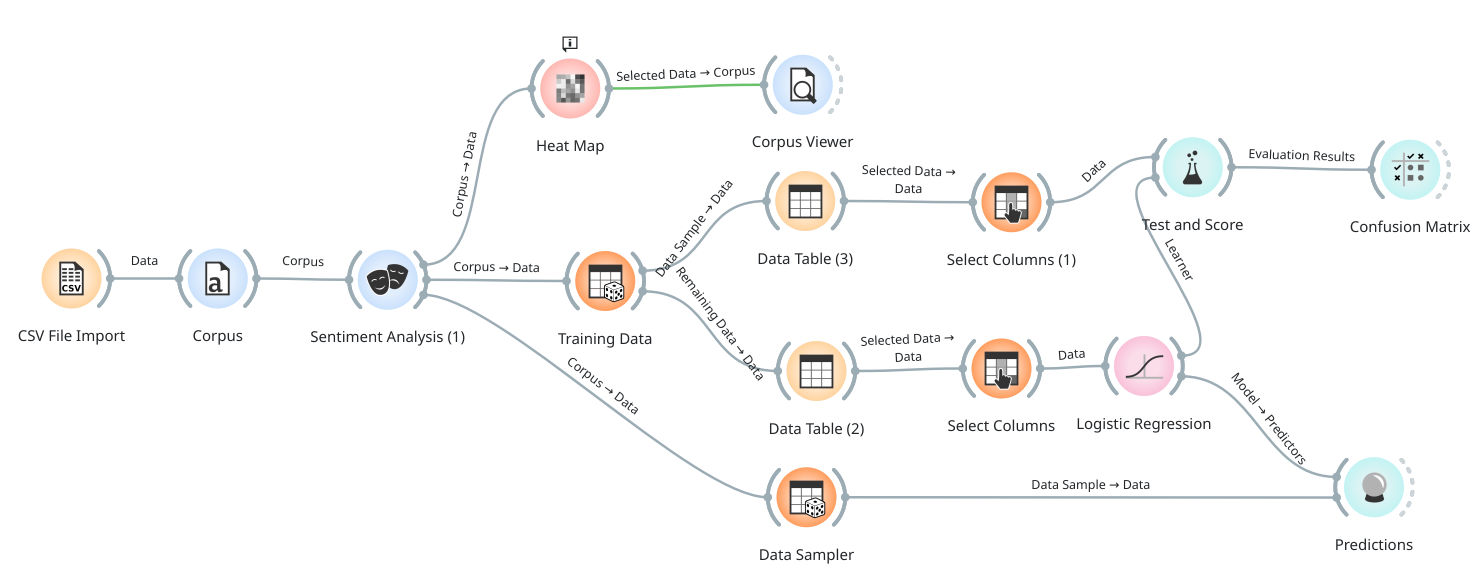
\includegraphics[width=\linewidth]{../figures/sentiment_pipeline.png}
	\caption{Pipeline untuk sentiment analysis menggunakan data Amazon dari UCI}
	\label{fig:sentiment-pipeline}
\end{figure}

\begin{enumerate}
	\item \textbf{CSV/Text File Import} \\
	Memuat dataset \texttt{amazon\_cells\_labelled.txt} (tab-delimited) yang berisi kolom teks ulasan dan label sentimen.
	
	\item \textbf{Corpus} \\
	Mengonversi data tabular menjadi \textit{Corpus}, memungkinkan pemrosesan teks lebih lanjut di Orange.
	
	\item \textbf{Sentiment Analysis} \\
	Menghitung skor sentimen (\textit{positive}, \textit{negative}, \textit{neutral}, dan \textit{compound}) per dokumen menggunakan pendekatan berbasis leksikon.
	
	\item \textbf{Heat Map} \\
	Visualisasi pola distribusi skor sentimen per dokumen dengan \textit{hierarchical clustering} untuk mengeksplor kemiripan ulasan.
	
	\item \textbf{Data Sampler → Training / Testing Data} \\
	Memisahkan data menjadi bagian pelatihan dan pengujian melalui widget \textit{Data Sampler}, sehingga dapat mengevaluasi model secara obyektif.
	
	\item \textbf{Select Columns} \\
	Memilih skor sentimen sebagai fitur, serta label sentimen sebagai target untuk pelatihan model.
	
	\item \textbf{Logistic Regression} \\
	Melatih model klasifikasi berdasarkan fitur skor sentimen.
	
	\item \textbf{Test \& Score} \\
	Mengevaluasi performa model terhadap data uji, menghasilkan metrik seperti:
	\begin{itemize}
		\item \textbf{CA} (Classification Accuracy),
		\item Precision, Recall, F1-score,
		\item AUC.
	\end{itemize}
	
	\item \textbf{Confusion Matrix} \\
	Menampilkan distribusi prediksi benar dan salah untuk tiap kategori sentimen.
	
	\item \textbf{Predictions} \\
	Menghasilkan dan menampilkan prediksi model untuk data baru atau diuji.
\end{enumerate}

\subsection*{Visualisasi Heatmap Skor Sentimen}

Gambar~\ref{fig:sentiment-heatmap} memperlihatkan hasil visualisasi \textit{heatmap} dari skor sentimen (\textit{positive}, \textit{negative}, \textit{neutral}, dan \textit{compound}) yang dihasilkan oleh widget \textit{Sentiment Analysis} untuk dataset Amazon.

Pada visualisasi ini:
\begin{itemize}
	\item Sumbu horizontal menunjukkan empat kategori skor sentimen:
	\begin{enumerate}
		\item \textbf{positive} — skor proporsi kata bernada positif dalam kalimat.
		\item \textbf{negative} — skor proporsi kata bernada negatif.
		\item \textbf{neutral} — skor proporsi kata netral.
		\item \textbf{compound} — skor gabungan dalam rentang $-1$ (sangat negatif) hingga $+1$ (sangat positif).
	\end{enumerate}
	
	\item Sumbu vertikal merepresentasikan setiap baris dokumen ulasan pada dataset, yang dikelompokkan secara hierarkis berdasarkan kemiripan profil skor sentimennya (\textit{hierarchical clustering}).
	
	\item Skala warna di bagian atas (biru $\rightarrow$ hijau $\rightarrow$ kuning) menunjukkan besar nilai skor:
	\begin{itemize}
		\item Biru = skor rendah atau negatif.
		\item Hijau = skor menengah.
		\item Kuning = skor tinggi atau positif.
	\end{itemize}
	
	\item Kotak hitam pada heatmap menandai kelompok dokumen yang memiliki pola skor sentimen yang serupa. Misalnya, pada kelompok yang ditandai, skor \textit{positive} dan \textit{neutral} relatif tinggi, sementara skor \textit{compound} rendah, yang mengindikasikan teks-teks tersebut mungkin mengandung campuran kata positif dan negatif sehingga skor akhir cenderung netral atau negatif.
\end{itemize}

Visualisasi seperti ini membantu dalam mengidentifikasi pola sentimen di antara ulasan, menemukan kelompok ulasan yang serupa, serta memberikan konteks tambahan sebelum data diproses ke tahap pelatihan model klasifikasi.

\begin{figure}[h]
	\centering
	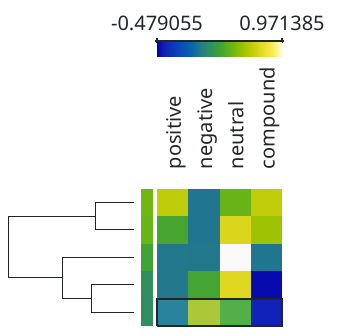
\includegraphics[width=0.5\linewidth]{../figures/sentiment_heatmap.png}
	\caption{Heatmap skor sentimen untuk dataset \texttt{amazon\_cells\_labelled.txt} dari UCI}
	\label{fig:sentiment-heatmap}
\end{figure}

\subsection*{Analisis Confusion Matrix}

Gambar~\ref{fig:sentiment-confmatrix} menunjukkan \textit{Confusion Matrix} hasil prediksi model \textit{Logistic Regression} terhadap dataset \texttt{amazon\_cells\_labelled.txt}. Confusion Matrix menampilkan distribusi jumlah prediksi benar dan salah untuk masing-masing kelas sentimen.

Pada matriks:
\begin{itemize}
	\item Baris merepresentasikan label \textbf{aktual} (ground truth).
	\item Kolom merepresentasikan label \textbf{prediksi} model.
	\item Kelas 0 = ulasan negatif, Kelas 1 = ulasan positif.
\end{itemize}

Hasil yang diperoleh:
\begin{itemize}
	\item \textbf{True Negative (TN)}: 45 ulasan negatif diprediksi benar sebagai negatif.
	\item \textbf{False Positive (FP)}: 5 ulasan negatif salah diprediksi sebagai positif.
	\item \textbf{False Negative (FN)}: 11 ulasan positif salah diprediksi sebagai negatif.
	\item \textbf{True Positive (TP)}: 39 ulasan positif diprediksi benar sebagai positif.
\end{itemize}

Interpretasi:
\begin{itemize}
	\item Model memiliki tingkat \textbf{akurasi} yang cukup tinggi, dengan mayoritas prediksi berada pada diagonal utama (TN dan TP).
	\item Hanya 16\% prediksi yang keliru (5 + 11 dari total 100 data uji).
	\item Kesalahan lebih banyak terjadi pada ulasan positif yang diklasifikasikan sebagai negatif (FN = 11) dibanding sebaliknya (FP = 5).
	\item Hal ini dapat mengindikasikan bahwa model sedikit lebih konservatif dalam memprediksi positif, atau beberapa ulasan positif mengandung kata-kata negatif yang kuat sehingga skor sentimennya bergeser.
\end{itemize}

\begin{figure}[h]
	\centering
	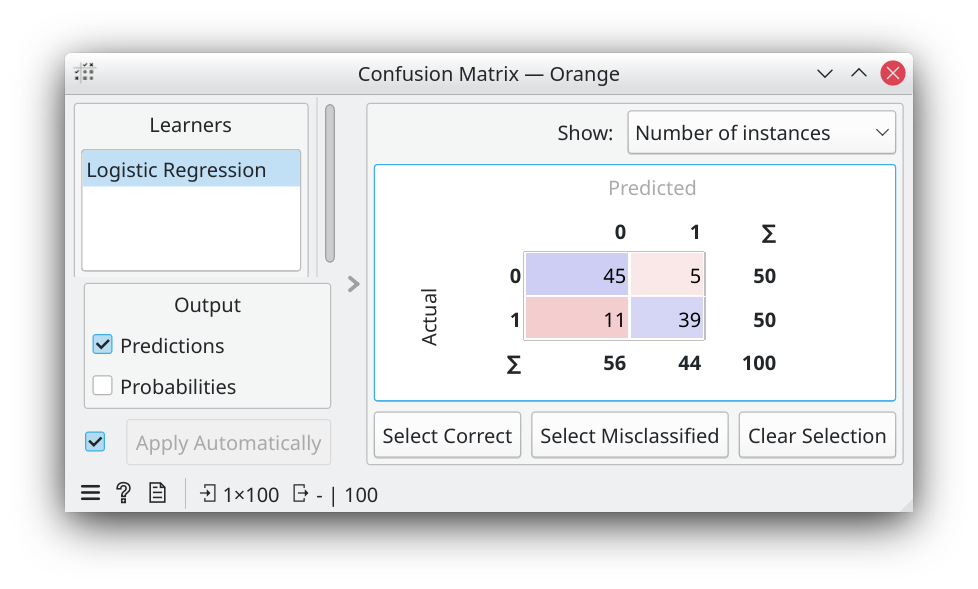
\includegraphics[width=0.6\linewidth]{../figures/sentiment_confusion_matrix.png}
	\caption{Confusion Matrix hasil prediksi Logistic Regression pada dataset \texttt{amazon\_cells\_labelled.txt}}
	\label{fig:sentiment-confmatrix}
\end{figure}


\subsection*{Evaluasi Model dengan Test and Score}

Evaluasi performa model klasifikasi dilakukan menggunakan widget \textit{Test and Score} pada Orange. Metode validasi yang digunakan adalah \textbf{cross-validation} dengan \textit{3-fold stratified}, yang memastikan distribusi kelas positif dan negatif seimbang di setiap fold pelatihan dan pengujian.

Gambar~\ref{fig:sentiment-testscore} menampilkan hasil evaluasi model \textit{Logistic Regression} terhadap dataset Amazon:

\begin{itemize}
	\item \textbf{AUC (Area Under Curve)} = 0.931 \\
	Menunjukkan kemampuan model membedakan kelas positif dan negatif. Nilai mendekati 1 berarti performa sangat baik.
	
	\item \textbf{CA (Classification Accuracy)} = 0.840 \\
	Persentase prediksi yang benar dari seluruh data uji, yaitu model berhasil mengklasifikasikan sekitar 84\% ulasan dengan benar.
	
	\item \textbf{F1-score} = 0.839 \\
	Rata-rata harmonis dari Precision dan Recall, merepresentasikan keseimbangan antara kedua metrik tersebut.
	
	\item \textbf{Precision} = 0.845 \\
	Proporsi prediksi positif yang benar-benar positif. Nilai ini menunjukkan sedikit di atas 84\% dari prediksi positif adalah benar.
	
	\item \textbf{Recall} = 0.840 \\
	Proporsi kasus positif yang berhasil dideteksi oleh model. Artinya, sekitar 84\% dari seluruh ulasan positif terklasifikasi dengan benar.
	
	\item \textbf{MCC (Matthews Correlation Coefficient)} = 0.685 \\
	Metrik korelasi antara prediksi dan label aktual, mempertimbangkan TP, TN, FP, dan FN. Nilai positif mendekati 1 menunjukkan korelasi yang kuat.
\end{itemize}

Dengan nilai AUC yang tinggi (0.931) dan akurasi yang stabil (0.840), dapat disimpulkan bahwa model Logistic Regression yang dibangun pada pipeline ini mampu mengklasifikasikan sentimen ulasan secara efektif pada dataset yang digunakan.

\begin{figure}[h]
	\centering
	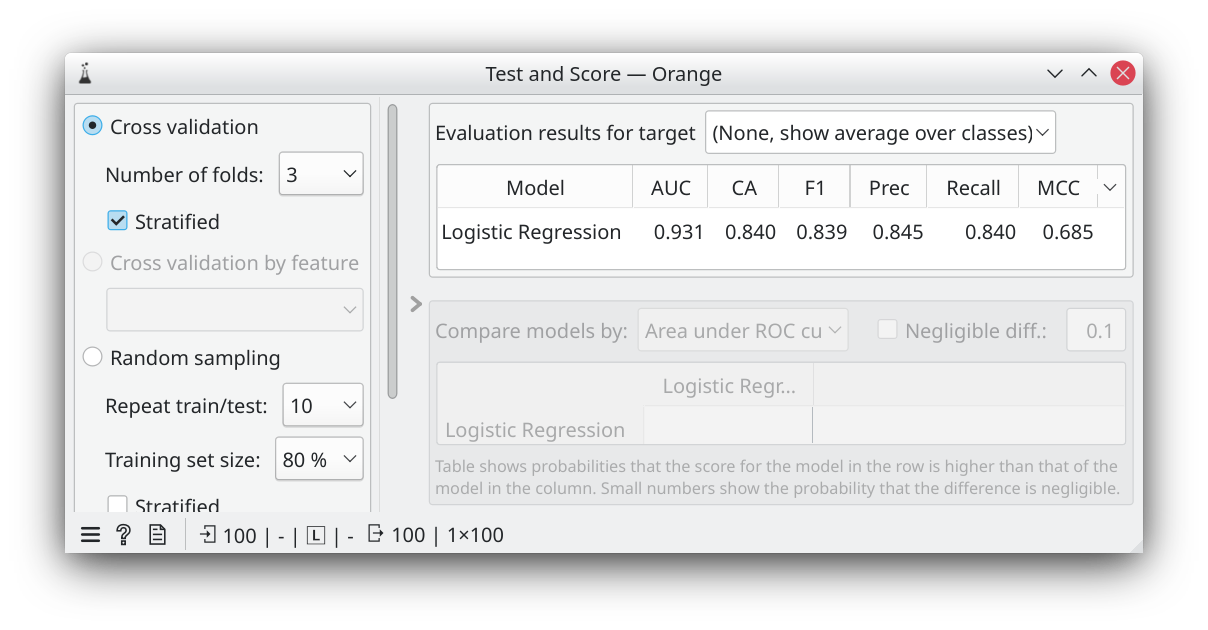
\includegraphics[width=0.75\linewidth]{../figures/sentiment_test.png}
	\caption{Hasil evaluasi model Logistic Regression menggunakan \textit{Test and Score} dengan 3-fold cross-validation pada dataset \texttt{amazon\_cells\_labelled.txt}}
	\label{fig:sentiment-testscore}
\end{figure}

\subsection*{Prediksi Sentimen pada Dataset}

Gambar~\ref{fig:sentiment-predictions} menampilkan keluaran dari widget \textit{Predictions} pada Orange, yang menunjukkan hasil prediksi model \textit{Logistic Regression} terhadap dataset \texttt{amazon\_cells\_labelled.txt}.

Widget \textit{Predictions} memberikan daftar label hasil prediksi untuk setiap entri teks dalam dataset, serta dapat menampilkan nilai probabilitas prediksi jika opsi tersebut diaktifkan. Pada kasus ini, tampilan memperlihatkan distribusi prediksi secara visual dalam bentuk warna untuk setiap baris data:
\begin{itemize}
	\item Setiap baris mewakili satu ulasan dari dataset.
	\item Warna mewakili kelas prediksi:
	\begin{itemize}
		\item Misalnya, oranye untuk prediksi \textbf{negatif} (0).
		\item Hijau untuk prediksi \textbf{positif} (1).
	\end{itemize}
	\item Urutan warna secara vertikal memperlihatkan urutan prediksi model terhadap keseluruhan dataset.
\end{itemize}

Dalam gambar, terlihat bahwa prediksi model tersebar antara kelas positif dan negatif, dengan pola warna yang relatif bervariasi. Hal ini menunjukkan bahwa dataset mengandung campuran ulasan positif dan negatif, serta model berhasil memisahkannya ke dalam dua kategori yang berbeda.

Widget ini berguna untuk:
\begin{itemize}
	\item Memeriksa hasil prediksi model terhadap data uji maupun data baru.
	\item Mengidentifikasi pola klasifikasi, misalnya jika terdapat bagian dataset yang didominasi oleh satu kelas tertentu.
	\item Mengekspor hasil prediksi untuk analisis lanjutan di luar Orange.
\end{itemize}

\begin{figure}[h]
	\centering
	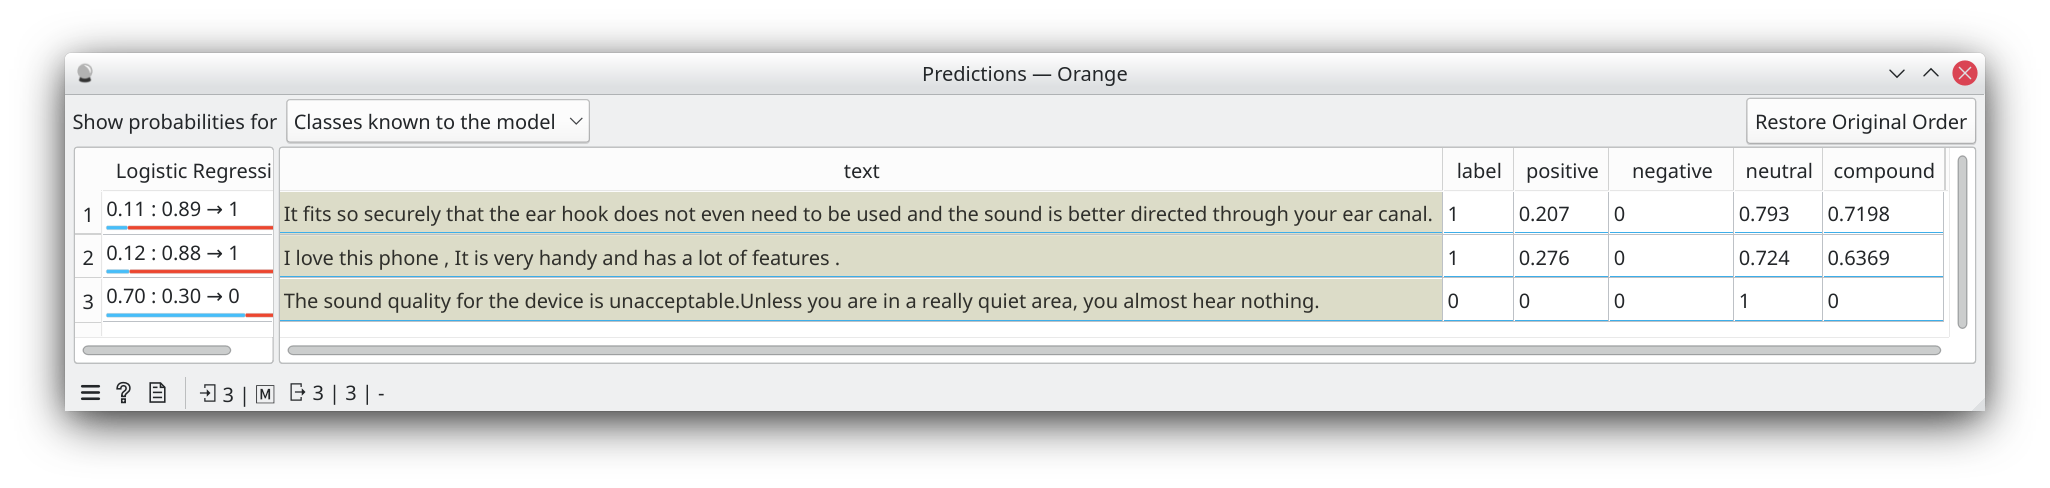
\includegraphics[width=\linewidth]{../figures/sentiment_prediction.png}
	\caption{Hasil prediksi model Logistic Regression terhadap dataset \texttt{amazon\_cells\_labelled.txt} ditampilkan menggunakan widget \textit{Predictions} di Orange}
	\label{fig:sentiment-predictions}
\end{figure}



\section{Interpretasi Hasil dan Strategi Bisnis}

Berdasarkan hasil analisis sentimen terhadap dataset \texttt{amazon\_cells\_labelled.txt} dari UCI Machine Learning Repository \cite{kotzias2015sentiment}, dapat disimpulkan beberapa temuan penting yang relevan untuk strategi bisnis.

\subsection*{Ringkasan Hasil Analisis}
\begin{itemize}
	\item \textbf{Heatmap Skor Sentimen} menunjukkan adanya kelompok ulasan dengan profil skor yang serupa, baik dari sisi skor positif, negatif, netral, maupun skor gabungan (\textit{compound}). Clustering ini dapat membantu mengidentifikasi segmen ulasan yang memiliki nuansa sentimen campuran, sehingga dapat dianalisis lebih lanjut untuk memahami faktor penyebabnya.
	\item \textbf{Evaluasi Model (Test and Score)} menghasilkan nilai AUC = 0.931, akurasi (CA) = 0.840, F1-score = 0.839, Precision = 0.845, dan Recall = 0.840. Nilai-nilai ini mengindikasikan bahwa model \textit{Logistic Regression} memiliki performa yang sangat baik dalam membedakan ulasan positif dan negatif pada dataset ini.
	\item \textbf{Confusion Matrix} memperlihatkan bahwa model melakukan prediksi benar pada 84\% data, dengan 45 ulasan negatif dan 39 ulasan positif terklasifikasi secara benar. Kesalahan lebih sering terjadi pada ulasan positif yang salah diprediksi sebagai negatif (FN = 11) dibandingkan sebaliknya (FP = 5).
	\item \textbf{Predictions} memperlihatkan distribusi prediksi positif dan negatif pada keseluruhan dataset, yang relatif seimbang. Hal ini mencerminkan distribusi kelas asli yang memang terdiri dari 50\% positif dan 50\% negatif.
\end{itemize}

\subsection*{Implikasi Strategi Bisnis}
Temuan di atas dapat diterjemahkan menjadi beberapa strategi bisnis yang aplikatif:
\begin{enumerate}
	\item \textbf{Pemantauan Kualitas Produk dan Layanan} \\
	Ulasan dengan skor sentimen negatif yang tinggi dapat diprioritaskan untuk dianalisis lebih lanjut. Kategori keluhan yang sering muncul dapat menjadi indikator area perbaikan, baik pada fitur produk maupun kualitas layanan pelanggan \cite{medhat2014sentiment}.
	\item \textbf{Peningkatan Retensi Pelanggan} \\
	Analisis pola pada ulasan positif yang konsisten dapat digunakan untuk mengidentifikasi faktor-faktor yang mendorong kepuasan pelanggan. Strategi retensi seperti program loyalitas dapat difokuskan pada aspek-aspek ini.
	\item \textbf{Segmentasi Pelanggan Berdasarkan Sentimen} \\
	Menggunakan hasil clustering dari heatmap, pelanggan dapat dikelompokkan ke dalam segmen sentimen spesifik (misalnya, sangat positif, campuran, atau sangat negatif). Setiap segmen dapat menerima komunikasi atau penawaran yang dipersonalisasi.
	\item \textbf{Pengukuran Dampak Perubahan Produk} \\
	Perubahan besar pada produk atau layanan (misalnya, peluncuran fitur baru) dapat dievaluasi dengan membandingkan distribusi sentimen sebelum dan sesudah implementasi \cite{liu2012sentiment}.
	\item \textbf{Integrasi dengan Sistem Otomatisasi} \\
	Model yang terlatih dapat diintegrasikan ke dalam sistem monitoring ulasan secara real-time untuk mendeteksi lonjakan sentimen negatif dan memberikan notifikasi cepat ke tim terkait.
\end{enumerate}

\subsection*{Keterbatasan dan Saran Pengembangan}
Walaupun model menunjukkan performa tinggi, beberapa keterbatasan tetap ada:
\begin{itemize}
	\item Dataset relatif kecil (1.000 ulasan) dan homogen (hanya produk ponsel dari Amazon), sehingga generalisasi ke domain lain perlu diuji.
	\item Analisis sentimen berbasis leksikon dapat kurang akurat untuk mendeteksi sarkasme, ironi, atau konteks bahasa yang kompleks \cite{pang2008opinion}.
	\item Model hanya mengklasifikasikan ke dalam dua kelas (positif dan negatif), padahal dalam praktik bisnis, kategori netral atau nuansa sentimen yang lebih halus juga penting.
\end{itemize}

Pengembangan selanjutnya dapat mencakup:
\begin{itemize}
	\item Menggunakan dataset yang lebih besar dan beragam.
	\item Mengadopsi model berbasis \textit{deep learning} seperti BERT untuk menangkap konteks kalimat yang lebih kompleks.
	\item Menambahkan analisis topik (\textit{topic modeling}) untuk memahami tema utama yang sering muncul pada ulasan dengan sentimen tertentu.
\end{itemize}

Dengan interpretasi hasil yang tepat, analisis sentimen seperti ini dapat menjadi landasan penting dalam pengambilan keputusan strategis, membantu bisnis untuk merespons masukan pelanggan secara proaktif, dan meningkatkan daya saing di pasar.


\section{Penutup}
Keseluruhan pembahasan menunjukkan bahwa analisis teks dan sentimen merupakan komponen penting dalam pemrosesan bahasa alami yang mampu mengubah data teks tidak terstruktur menjadi wawasan strategis. Mulai dari tahap pengumpulan dan prapemrosesan data, ekstraksi fitur, hingga pemilihan metode klasifikasi, setiap langkah memiliki peran krusial dalam menghasilkan model yang akurat. Beragam pendekatan—mulai dari berbasis kamus, pembelajaran mesin, hingga pembelajaran mendalam—menawarkan keunggulan dan keterbatasannya masing-masing, sehingga pemilihan metode harus mempertimbangkan tujuan analisis, ketersediaan data, serta sumber daya komputasi. Studi kasus ulasan produk e-commerce menegaskan bagaimana analisis sentimen dapat membantu mengidentifikasi pola persepsi pelanggan secara kuantitatif, sekaligus memandu strategi perbaikan dan inovasi.

Hasil implementasi menggunakan dataset publik Amazon dan alat visual Orange menunjukkan performa model yang tinggi, dengan AUC mencapai 0.931 dan akurasi 84\%. Visualisasi seperti heatmap dan confusion matrix memperkaya pemahaman terhadap distribusi sentimen serta pola kesalahan prediksi. Implikasi bisnis dari temuan ini sangat luas, mulai dari pemantauan kualitas produk, peningkatan retensi pelanggan, hingga segmentasi berbasis sentimen. Meskipun terdapat keterbatasan, seperti ukuran dataset yang kecil dan domain yang spesifik, pendekatan ini tetap menawarkan fondasi yang kuat bagi pengambilan keputusan berbasis data. Dengan pengembangan lebih lanjut, termasuk penggunaan model kontekstual seperti BERT dan dataset yang lebih beragam, analisis sentimen dapat menjadi alat prediktif dan diagnostik yang semakin andal dalam ekosistem bisnis modern.
%	\chapter{Penutup}

Penggunaan Large Language Model (LLM) dalam dunia pendidikan membuka peluang baru untuk mentransformasi cara guru mengajar, merancang pembelajaran, memberikan umpan balik, hingga mengelola tugas-tugas administratif. Melalui enam bab sebelumnya, buku ini telah mengajak pembaca mengeksplorasi berbagai aplikasi praktis LLM mulai dari mendesain materi ajar, memberikan penilaian yang responsif, hingga mengelola komunikasi dan dokumen secara otomatis.

Pengenalan LLM di kelas bukan sekadar tren teknologi, tetapi bagian dari proses adaptasi terhadap kebutuhan pembelajaran yang semakin kompleks dan beragam. Dengan memahami cara kerja dan potensi LLM, guru dapat lebih percaya diri menggunakan AI sebagai mitra untuk meningkatkan kualitas pembelajaran, bukan sebagai pengganti peran edukatif mereka.

Namun, adopsi teknologi juga membawa tantangan etis dan risiko yang perlu disikapi dengan bijak. Bab tentang etika menjadi pengingat penting bahwa kecanggihan teknologi harus selalu diimbangi dengan pertimbangan nilai, tanggung jawab, dan perlindungan terhadap peserta didik.

Sebagai penutup, diharapkan pembaca tidak hanya memperoleh pemahaman teknis dan praktis tentang LLM, tetapi juga membangun refleksi kritis dan kesadaran profesional dalam penggunaannya. Teknologi hanyalah alat; dampak positifnya tergantung pada bagaimana dan untuk tujuan apa ia digunakan.

Mari terus belajar, bereksperimen, dan bertumbuh bersama AI—dengan tetap menempatkan nilai-nilai pendidikan sebagai fondasi utama dalam setiap langkah transformasi digital di kelas.



	\backmatter
	\addcontentsline{toc}{chapter}{Daftar Pustaka}
	\bibliographystyle{plain}
	\bibliography{references}
	
\end{document}